% rubber: bibtex.crossrefs 10000
\documentclass[a4paper,12pt,oneside,minionpro,dottedtoc]{thesis}

\usepackage[a4paper,left=2cm,right=2cm,top=2cm,bottom=3cm]{geometry}

\title{Multi-version Software Updates}
\author{Petr Hosek}
\date{December 2014}
\university{Imperial College London}
\department{Department of Computing}
\supervisor{Dr Cristian Cadar}
\dedication{}

\lstset{
  language=C,
  captionpos=b,
  basicstyle=\small\ttfamily,
  commentstyle=\textit,
  keywordstyle=\bfseries,
  numbers=left,
  numberstyle=\small,
  numbersep=5pt,
  escapeinside={/*@}{@*/},
  tabsize=2,
  breaklines=true,
  extendedchars=true,
  columns=fullflexible,
  xleftmargin=16pt,
  showspaces=false,
  showtabs=false,
  showstringspaces=false,
  moredelim=**[is][\bfseries]{@}{@},
}

\lstdefinelanguage
   [x64]{Assembler}
   [x86masm]{Assembler}
   {morekeywords={CDQE,CQO,CMPSQ,CMPXCHG16B,JRCXZ,LODSQ,MOVSXD,%
                  POPFQ,PUSHFQ,SCASQ,STOSQ,IRETQ,RDTSCP,SWAPGS,%
                  SYSCALL,SYSRET,SYSENTER,SYSEXIT,%
                  rax,rdx,rcx,rbx,rsi,rdi,rsp,rbp,%
                  r8,r8d,r8w,r8b,r9,r9d,r9w,r9b}}

\lstdefinelanguage
  [bpf]{Assembler}
  {morekeywords={ldb,ldh,ld,ldi,ldx,ldxi,ldxb,st,stx,jmp,ja,jeq,jneq,%
                 jne,jlt,jle,jgt,jge,jset,add,sub,mul,div,mod,neg,and,xor,or,%
                 lsh,rsh,ret,tax,txa},%
   alsoletter=.,alsodigit=?,%
   sensitive=false,%
   morestring=[b]",%
   morestring=[b]',%
   morecomment=[l];%
   }[keywords,comments,strings]

\usepackage[binary-units,group-separator={,}]{siunitx}
\sisetup{per-mode=symbol}
\DeclareSIUnit[number-unit-product=\,]{\loc}{LOC}

\usepackage{xspace}
\usepackage{url}
\usepackage[normalem]{ulem}
\usepackage{multirow}
\usepackage{paralist}
\setlength{\parskip}{0cm}
\setlength{\parindent}{1em}

\usepackage[backend=biber,style=alphabetic,mincrossrefs=10000]{biblatex}
\addbibresource{bibliography/cadar-macros.bib}
\addbibresource{bibliography/cadar-crossrefs.bib}
\addbibresource{bibliography/cadar.bib}

\newcommand*\circl[1]{%
  \begin{tikzpicture}[baseline=(C.base)]
    \node[draw,circle,inner sep=0.25pt](C) {#1};
  \end{tikzpicture}}

\newcommand{\boldtext}[1]{\vspace{0.05in}\noindent\textbf{#1}}
\newcommand{\textstt}[1]{{\small \texttt{#1}}\xspace}
%\newcommand{\textssc}[1]{{\small \textsc{#1}}\xspace}
\newcommand{\textssc}[1]{\textls[80]{\scshape\MakeTextLowercase{#1}}}

\newcommand{\mx}[0]{\textsc{Mx}\xspace}
\newcommand{\mxe}[0]{\textsc{MxE}\xspace}
\newcommand{\sea}[0]{\textsc{Sea}\xspace}
\newcommand{\rem}[0]{\textsc{Rem}\xspace}
\newcommand{\mxm}[0]{\textsc{Mxm}\xspace}
\newcommand{\mv}[0]{\textsc{MV}\xspace}

\newcommand{\ptrace}[0]{\stt{ptrace}\xspace}
\newcommand{\redisbenchmark}[0]{\textstt{redis-benchmark}}
\newcommand{\httpload}[0]{\textstt{http\_load}}
\newcommand{\spec}[0]{\textit{SPEC~CPU2006}\xspace}
\newcommand{\vsftpd}[0]{\emph{vsftpd}\xspace}
\newcommand{\vim}[0]{\emph{Vim}\xspace}
\newcommand{\gchrome}[0]{\emph{Google Chrome}\xspace}
\newcommand{\chrome}[0]{\emph{Chrome}\xspace}
\newcommand{\coreutils}[0]{\emph{Coreutils}\xspace}

\newcommand{\binutils}[0]{\textit{Binutils}\xspace}
\newcommand{\gnu}[0]{\textit{GNU}\xspace}
\newcommand{\mdsum}[0]{\textstt{md5sum}}
\newcommand{\shasum}[0]{\textstt{sha1sum}}
\newcommand{\mkdir}[0]{\textstt{mkdir}}
\newcommand{\mkfifo}[0]{\textstt{mkfifo}}
\newcommand{\mknod}[0]{\textstt{mknod}}
\newcommand{\cut}[0]{\textstt{cut}}

\newcommand{\todo}[1]{\noindent{\color{red}[{\bf todo:} #1]}}
\newcommand{\sidenote}[1]{{\marginpar{\bf\color{red}[#1]}}}
\newcommand{\gap}[2]{\uline{#1} \noindent{\color{red}[#2]}}

\newenvironment{structure}{\color{blue}
\begin{list}{\labelitemi}{\leftmargin=1em}{%
\setlength{\topsep}{0pt}\setlength{\itemsep}{0pt}\setlength{\parsep}{0pt}}}
{\end{list}}

\newenvironment{structure*}{\color{blue}
\begin{enumerate}\setlength{\topsep}{0pt}\setlength{\itemsep}{0pt}\setlength{\parsep}{0pt}}
{\end{enumerate}}

\newcommand{\ie}{\emph{i.e.}\ }
\newcommand{\eg}{\emph{e.g.},\ }
\newcommand{\etal}{\emph{et al.}\ }
\newcommand{\vs}{\emph{vs.}\ }
\newcommand{\etc}{\emph{etc.}\ }
\newcommand{\resp}{\emph{resp.}\ }

\newcommand{\sref}[1]{\S\ref{#1}}

%%%

\newcounter{enumcount}
\newenvironment{enumnoind}
 {\begin{list}{(\arabic{enumcount})~~}{\usecounter{enumcount} 
  \labelsep=0em \labelwidth=0em \leftmargin=0em \itemindent=0em}}
 {\end{list}}

\definecolor{lightGrey}{rgb}{0.8, 0.8, 0.8}
\newcommand{\Hilight}{\makebox[0pt][l]{\color{lightGrey}\rule[-0.45em]{\linewidth}{1.5em}}}
\newcommand{\topic}{}

\hyphenation{ex-e-cu-tion}
\hyphenation{non-de-ter-min-is-tic}

\newcommand{\stt}[1]{\texttt{\small #1}}
\newcommand{\heading}[1]{\vspace{0.1in} \noindent \textit{#1}}

\newcommand{\hl}[1]{\textit{\textbf{#1}}}
%\newcommand{\hl}[1]{#1}

\newcommand{\covrig}{\textsc{Covrig}\xspace}
\newcommand{\katch}{\textsc{katch}\xspace}
\newcommand{\klee}{\textsc{klee}\xspace}
\newcommand{\llvm}{\textsc{llvm}\xspace}
\newcommand{\stp}{\textsc{stp}\xspace}
\newcommand{\symex}{\textsc{SE}\xspace}
\newcommand{\zesti}{\textsc{zesti}\xspace}

\newcommand{\diff}{\stt{diff}\xspace}
\newcommand{\gcov}{\stt{gcov}\xspace}
\newcommand{\eloc}{\xspace{\small ELOC}\xspace}

\newcommand{\diffutils}{Diffutils\xspace}
\newcommand{\findutils}{Findutils\xspace}
\newcommand{\zeromq}{{\O}MQ\xspace}
\newcommand{\git}{Git\xspace}

\newcommand{\true}{\stt{true}\xspace}
\newcommand{\false}{\stt{false}\xspace}

\newcommand{\nx}[0]{\textsc{Varan}\xspace}
\newcommand{\vx}[0]{\textsc{Vx}\xspace}
\newcommand{\varan}[0]{\textsc{Varan}\xspace}
\newcommand{\nxlib}[0]{\textsc{VaranLib}\xspace}

\newcommand{\linux}{Linux\xspace}
\newcommand{\docker}{Docker\xspace}
\newcommand{\fabric}{Fabric\xspace}
\newcommand{\lxc}{LXC\xspace}
\newcommand{\github}{GitHub\xspace}
\newcommand{\cloudstack}{CloudStack\xspace}
\newcommand{\xen}{Xen\xspace}
\newcommand{\kvm}{KVM\xspace}

\newcommand{\apache}[0]{\textit{Apache httpd}\xspace}
\newcommand{\httpd}[0]{\textit{Apache httpd}\xspace}
\newcommand{\beanstalkd}[0]{\textit{Beanstalkd}\xspace}
\newcommand{\lighttpd}[0]{\textit{lighttpd}\xspace}
\newcommand{\lighttpdtwo}[0]{\textit{lighttpd~2.0}\xspace}
\newcommand{\memcached}[0]{\textit{Memcached}\xspace}
\newcommand{\nginx}[0]{\textit{Nginx}\xspace}
\newcommand{\redis}[0]{\textit{Redis}\xspace}
\newcommand{\speccpu}[0]{\textit{SPEC CPU}\xspace}
\newcommand{\speczerozero}[0]{\textit{SPEC CPU2000}\xspace}
\newcommand{\speczerosix}[0]{\textit{SPEC CPU2006}\xspace}
\newcommand{\thttpd}[0]{\textit{thttpd}\xspace}
\newcommand{\gdb}[0]{\textit{GDB}\xspace}

\newcommand{\orchestra}[0]{\textit{Orchestra}\xspace}
\newcommand{\scribe}[0]{\textit{Scribe}\xspace}
\newcommand{\strata}[0]{\textit{Strata}\xspace}
\newcommand{\tachyon}[0]{\textit{Tachyon}\xspace}

\usepackage{hyperref}
\hypersetup{
  unicode=true,
  bookmarksopen=true,
  bookmarksnumbered=true,
  linktoc=page,
  colorlinks=true,
  linkcolor=pantone186,
  citecolor=pantone334,
  urlcolor=pantone527
}

%%%

\newcounter{coverage}
\newtheorem{question}[coverage]{RQ}
\let\savedquestion\question % unicode-math#271 workaround

\newcommand{\rqone}{Do executable and test code evolve in sync?}
\newcommand{\rqtwo}{How many patches touch only code, only tests, none, or both?}
\newcommand{\rqthree}{What is the distribution of patch sizes? How spread out is each patch through the code?}
\newcommand{\rqfour}{Is test suite execution deterministic?}
\newcommand{\rqfive}{How does the overall code coverage evolve?  Is it stable over time?}
\newcommand{\rqsix}{What is the distribution of patch coverage across revisions?}
\newcommand{\rqseven}{What fraction of patch code is tested within a few revisions after it is added, \ie what is the {\em latent patch coverage}?}
\newcommand{\rqeight}{Are bug fixes better covered than other types of patches?}
\newcommand{\rqnine}{Is the coverage of buggy code less than average?}

\newcommand{\numSystems}[0]{six\xspace}
\newcommand{\numYears}[0]{twelve\xspace}

%%these are wall-clock times
\newcommand{\redisCompileTime}[0]{19\xspace}
\newcommand{\redisTestTime}[0]{315\xspace}

\newcommand{\zeromqCompileTime}[0]{21\xspace}
\newcommand{\zeromqTestTime}[0]{10\xspace}

\newcommand{\lighttpdtwoCompileTime}[0]{17\xspace}
\newcommand{\lighttpdtwoTestTime}[0]{3\xspace}

\newcommand{\memcachedCompileTime}[0]{9\xspace}
\newcommand{\memcachedTestTime}[0]{110\xspace}

\newcommand{\binutilsCompileTime}[0]{43\xspace}
\newcommand{\binutilsTestTime}[0]{10\xspace}

\newcommand{\gitCompileTime}[0]{49\xspace}
\newcommand{\gitTestTime}[0]{1836\xspace}

\newcommand{\memcachedOriginsLineCoverage}[0]{44.1\%\xspace}
\newcommand{\memcachedOriginsInRange}[0]{24}
\newcommand{\memcachedOriginsOutOfRange}[0]{21\xspace}

\newcommand{\redisOriginsLineCoverage}[0]{52.8\%\xspace}
\newcommand{\redisOriginsInRange}[0]{9}
\newcommand{\redisOriginsOutOfRange}[0]{11}

\newcommand{\zeromqOriginsLineCoverage}[0]{43.3\%\xspace}
\newcommand{\zeromqOriginsInRange}[0]{14}
\newcommand{\zeromqOriginsOutOfRange}[0]{30}

%\newcommand{\memcachedBugs}[0]{45\xspace}
%\newcommand{\memcachedFixCoverage}[0]{72\%\xspace}
%\newcommand{\memcachedBugCoverage}[0]{78\%\xspace}
%\newcommand{\memcachedBugsFullyCovered}[0]{25\xspace}
%\newcommand{\memcachedFixesFullyCovered}[0]{28\xspace}
%\newcommand{\memcachedFixesWithoutCode}[0]{4\xspace}
%\newcommand{\memcachedBugsWithoutCode}[0]{5\xspace}
%
%\newcommand{\zeromqBugs}[0]{25\xspace}
%\newcommand{\zeromqFixCoverage}[0]{46\%\xspace}
%\newcommand{\zeromqBugCoverage}[0]{50\%\xspace}
%\newcommand{\zeromqFixesFullyCovered}[0]{10\xspace}
%\newcommand{\zeromqBugsFullyCovered}[0]{13\xspace}
%\newcommand{\zeromqFixesWithoutCode}[0]{3\xspace}
%\newcommand{\zeromqBugsWithoutCode}[0]{5\xspace}
%
%\newcommand{\redisBugs}[0]{25\xspace}
%\newcommand{\redisFixCoverage}[0]{63\%\xspace}
%\newcommand{\redisBugCoverage}[0]{67\%\xspace}
%\newcommand{\redisFixesFullyCovered}[0]{14\xspace}
%\newcommand{\redisBugsFullyCovered}[0]{13\xspace}
%\newcommand{\redisFixesWithoutCode}[0]{3\xspace}
%\newcommand{\redisBugsWithoutCode}[0]{4\xspace}

%% beanstalkd@https://github.com/kr/beanstalkd.git
%% beanstalkd: 250 actual revisions (261845d - fb0a466)
\newcommand{\beanstalkdRevs}[0]{250\xspace}
\newcommand{\beanstalkdTimespan}[0]{\xspace}
\newcommand{\beanstalkdSize}[0]{2,567\xspace}
\newcommand{\beanstalkdTsize}[0]{2,031\xspace}
\newcommand{\beanstalkdDeltaSize}[0]{822\xspace}
\newcommand{\beanstalkdInitialCoverage}[0]{32.20\%\xspace}
\newcommand{\beanstalkdFinalCoverage}[0]{5.25\%\xspace}
\newcommand{\beanstalkdTransientCompErrs}[0]{7\xspace}
\newcommand{\beanstalkdTransientTestErrs}[0]{99\xspace}
\newcommand{\beanstalkdTransientTestTimeouts}[0]{0\xspace}
\newcommand{\beanstalkdOK}[0]{151\xspace}
\newcommand{\beanstalkdMerges}[0]{8\xspace}

\newcommand{\beanstalkdOnlyTestRevs}[0]{38\xspace}
\newcommand{\beanstalkdOnlyExecutableRevs}[0]{155\xspace}
\newcommand{\beanstalkdTestAndExecutableRevs}[0]{57\xspace}
\newcommand{\beanstalkdNoTestNoExecutableRevs}[0]{156\xspace}

\newcommand{\beanstalkdFullyCoveredPercent}[0]{11.3\%\xspace}
\newcommand{\beanstalkdZeroCoveredPercent}[0]{61.7\%\xspace}
\newcommand{\beanstalkdOneELOCPatches}[0]{23.1\%\xspace}
\newcommand{\beanstalkdOneeHunkPatches}[0]{33.0\%\xspace}
\newcommand{\beanstalkdOneeFilePatches}[0]{65.0\%\xspace}
\newcommand{\beanstalkdCovLines}[0]{1,167\xspace}
\newcommand{\beanstalkdUncovLines}[0]{3,428\xspace}
\newcommand{\beanstalkdPatchTotal}[0]{4,595\xspace}
\newcommand{\beanstalkdeHunkZeroTotal}[0]{1,801\xspace}
\newcommand{\beanstalkdeHunkThreeTotal}[0]{1,140\xspace}
\newcommand{\beanstalkdeFileTotal}[0]{406\xspace}

\newcommand{\beanstalkdPatchAverage}[0]{21.67\xspace}
\newcommand{\beanstalkdPatchMedian}[0]{4\xspace}
\newcommand{\beanstalkdPatchMode}[0]{1\xspace}
\newcommand{\beanstalkdPatchStdev}[0]{52.85\xspace}

\newcommand{\beanstalkdeHunkZeroAverage}[0]{8.49\xspace}
\newcommand{\beanstalkdeHunkZeroMedian}[0]{3\xspace}
\newcommand{\beanstalkdeHunkZeroMode}[0]{1\xspace}
\newcommand{\beanstalkdeHunkZeroStdev}[0]{15.76\xspace}

\newcommand{\beanstalkdeHunkThreeAverage}[0]{5.37\xspace}
\newcommand{\beanstalkdeHunkThreeMedian}[0]{2\xspace}
\newcommand{\beanstalkdeHunkThreeMode}[0]{1\xspace}
\newcommand{\beanstalkdeHunkThreeStdev}[0]{8.45\xspace}

\newcommand{\beanstalkdeFileAverage}[0]{1.91\xspace}
\newcommand{\beanstalkdeFileMedian}[0]{1\xspace}
\newcommand{\beanstalkdeFileMode}[0]{1\xspace}
\newcommand{\beanstalkdeFileStdev}[0]{1.89\xspace}

\newcommand{\beanstalkdCoverageAverage}[0]{22.19\%\xspace}
\newcommand{\beanstalkdCoverageMedian}[0]{25.42\%\xspace}
\newcommand{\beanstalkdCoverageMode}[0]{28.17\%\xspace}
\newcommand{\beanstalkdCoverageStdev}[0]{7.74pp\xspace}

\newcommand{\beanstalkdBranchCoverageAverage}[0]{12.00\%\xspace}
\newcommand{\beanstalkdBranchCoverageMedian}[0]{12.67\%\xspace}
\newcommand{\beanstalkdBranchCoverageMode}[0]{13.39\%\xspace}
\newcommand{\beanstalkdBranchCoverageStdev}[0]{4.51pp\xspace}

\newcommand{\beanstalkdPatchCovEntries}[0]{212\xspace}
\newcommand{\beanstalkdPatchCovAverage}[0]{22\%\xspace}
\newcommand{\beanstalkdPatchCovMedian}[0]{0\%\xspace}
\newcommand{\beanstalkdPatchCovMode}[0]{0\xspace}
\newcommand{\beanstalkdPatchCovStdev}[0]{35pp\xspace}

\newcommand{\beanstalkdPatchCovEntriesZero}[0]{146\xspace}
\newcommand{\beanstalkdPatchCovAverageZero}[0]{19\%\xspace}
\newcommand{\beanstalkdPatchCovMedianZero}[0]{0\%\xspace}
\newcommand{\beanstalkdPatchCovModeZero}[0]{0\xspace}
\newcommand{\beanstalkdPatchCovStdevZero}[0]{36pp\xspace}

\newcommand{\beanstalkdPatchCovEntriesTen}[0]{55\xspace}
\newcommand{\beanstalkdPatchCovAverageTen}[0]{27\%\xspace}
\newcommand{\beanstalkdPatchCovMedianTen}[0]{11\%\xspace}
\newcommand{\beanstalkdPatchCovModeTen}[0]{0\xspace}
\newcommand{\beanstalkdPatchCovStdevTen}[0]{32pp\xspace}

\newcommand{\beanstalkdPatchCovEntriesHundred}[0]{11\xspace}
\newcommand{\beanstalkdPatchCovAverageHundred}[0]{23\%\xspace}
\newcommand{\beanstalkdPatchCovMedianHundred}[0]{4\%\xspace}
\newcommand{\beanstalkdPatchCovModeHundred}[0]{\xspace}
\newcommand{\beanstalkdPatchCovStdevHundred}[0]{33pp\xspace}

\newcommand{\beanstalkdOverallPatchCovEntriesZero}[0]{146\xspace}
\newcommand{\beanstalkdOverallPatchCovZero}[0]{19.8\%\xspace}

\newcommand{\beanstalkdOverallPatchCovEntriesTen}[0]{55\xspace}
\newcommand{\beanstalkdOverallPatchCovTen}[0]{28.3\%\xspace}

\newcommand{\beanstalkdOverallPatchCovEntriesHundred}[0]{11\xspace}
\newcommand{\beanstalkdOverallPatchCovHundred}[0]{24.1\%\xspace}

\newcommand{\beanstalkdOverallPatchCoverage}[0]{25.3\%\xspace}
\newcommand{\beanstalkdLatentOne}[0]{.4\%\xspace}
\newcommand{\beanstalkdLatentFive}[0]{.4\%\xspace}
\newcommand{\beanstalkdLatentTen}[0]{.6\%\xspace}

\newcommand{\beanstalkdRevsAllTestsFailed}[0]{97\xspace}
\newcommand{\beanstalkdRevsAllTestsOK}[0]{150\xspace}
\newcommand{\beanstalkdRevsTestsMixedResults}[0]{3\xspace}
%\renewcommand{\beanstalkdTransientTestErrs}[0]{3\xspace}
\newcommand{\beanstalkdNonDetMax}[0]{17\xspace}
\newcommand{\beanstalkdNonDetAverage}[0]{0.17\xspace}
\newcommand{\beanstalkdNonDetMedian}[0]{0\xspace}
\newcommand{\beanstalkdNonDetMode}[0]{0\xspace}
\newcommand{\beanstalkdNonDetStdev}[0]{1.57\xspace}
\newcommand{\beanstalkdNonDetCount}[0]{247\xspace}


%% binutils@git://sourceware.org/git/binutils.git
%%  3950/381/303 all/affecting binutils not compiling/affecting binutils compiling revisions (4343fe0 - a0a1bb0), 60sec timeout
%% binutils: 250 actual revisions (3d62a77 - 2b9ed0a)
\newcommand{\binutilsRevs}[0]{250\xspace}
\newcommand{\binutilsTimespan}[0]{35\xspace}
\newcommand{\binutilsSize}[0]{27,029\xspace}
\newcommand{\binutilsTsize}[0]{5,186\xspace}
\newcommand{\binutilsDeltaSize}[0]{1,657\xspace}
\newcommand{\binutilsInitialCoverage}[0]{16.94\%\xspace}
\newcommand{\binutilsFinalCoverage}[0]{17.81\%\xspace}
\newcommand{\binutilsTransientCompErrs}[0]{25\xspace}
\newcommand{\binutilsTransientTestErrs}[0]{10\xspace}
\newcommand{\binutilsTransientTestTimeouts}[0]{0\xspace}
\newcommand{\binutilsOK}[0]{240\xspace}
\newcommand{\binutilsMerges}[0]{0\xspace}

\newcommand{\binutilsOnlyTestRevs}[0]{50\xspace}
\newcommand{\binutilsOnlyExecutableRevs}[0]{180\xspace}
\newcommand{\binutilsTestAndExecutableRevs}[0]{20\xspace}
\newcommand{\binutilsNoTestNoExecutableRevs}[0]{124\xspace}

\newcommand{\binutilsFullyCoveredPercent}[0]{12.0\%\xspace}
\newcommand{\binutilsOneELOCPatches}[0]{20.5\%\xspace}
\newcommand{\binutilsOneeHunkPatches}[0]{34.5\%\xspace}
\newcommand{\binutilsOneeFilePatches}[0]{88.5\%\xspace}
\newcommand{\binutilsCovLines}[0]{883\xspace}
\newcommand{\binutilsUncovLines}[0]{3,272\xspace}
\newcommand{\binutilsPatchTotal}[0]{4,155\xspace}
\newcommand{\binutilseHunkZeroTotal}[0]{2,124\xspace}
\newcommand{\binutilseHunkThreeTotal}[0]{1,288\xspace}
\newcommand{\binutilseFileTotal}[0]{246\xspace}

\newcommand{\binutilsPatchAverage}[0]{20.77\xspace}
\newcommand{\binutilsPatchMedian}[0]{5\xspace}
\newcommand{\binutilsPatchMode}[0]{1\xspace}
\newcommand{\binutilsPatchStdev}[0]{41.56\xspace}

\newcommand{\binutilseHunkZeroAverage}[0]{10.62\xspace}
\newcommand{\binutilseHunkZeroMedian}[0]{3\xspace}
\newcommand{\binutilseHunkZeroMode}[0]{1\xspace}
\newcommand{\binutilseHunkZeroStdev}[0]{22.51\xspace}

\newcommand{\binutilseHunkThreeAverage}[0]{6.44\xspace}
\newcommand{\binutilseHunkThreeMedian}[0]{2\xspace}
\newcommand{\binutilseHunkThreeMode}[0]{1\xspace}
\newcommand{\binutilseHunkThreeStdev}[0]{12.29\xspace}

\newcommand{\binutilseFileAverage}[0]{1.23\xspace}
\newcommand{\binutilseFileMedian}[0]{1\xspace}
\newcommand{\binutilseFileMode}[0]{1\xspace}
\newcommand{\binutilseFileStdev}[0]{0.81\xspace}

\newcommand{\binutilsCoverageAverage}[0]{17.39\%\xspace}
\newcommand{\binutilsCoverageMedian}[0]{17.47\%\xspace}
\newcommand{\binutilsCoverageMode}[0]{17.69\%\xspace}
\newcommand{\binutilsCoverageStdev}[0]{0.35pp\xspace}

\newcommand{\binutilsBranchCoverageAverage}[0]{13.20\%\xspace}
\newcommand{\binutilsBranchCoverageMedian}[0]{13.23\%\xspace}
\newcommand{\binutilsBranchCoverageMode}[0]{13.41\%\xspace}
\newcommand{\binutilsBranchCoverageStdev}[0]{0.20pp\xspace}

\newcommand{\binutilsPatchCovEntries}[0]{200\xspace}
\newcommand{\binutilsPatchCovAverage}[0]{25\%\xspace}
\newcommand{\binutilsPatchCovMedian}[0]{0\%\xspace}
\newcommand{\binutilsPatchCovMode}[0]{0\xspace}
\newcommand{\binutilsPatchCovStdev}[0]{35pp\xspace}

\newcommand{\binutilsPatchCovEntriesZero}[0]{128\xspace}
\newcommand{\binutilsPatchCovAverageZero}[0]{25\%\xspace}
\newcommand{\binutilsPatchCovMedianZero}[0]{0\%\xspace}
\newcommand{\binutilsPatchCovModeZero}[0]{0\xspace}
\newcommand{\binutilsPatchCovStdevZero}[0]{38pp\xspace}

\newcommand{\binutilsPatchCovEntriesTen}[0]{63\xspace}
\newcommand{\binutilsPatchCovAverageTen}[0]{27\%\xspace}
\newcommand{\binutilsPatchCovMedianTen}[0]{12\%\xspace}
\newcommand{\binutilsPatchCovModeTen}[0]{0\xspace}
\newcommand{\binutilsPatchCovStdevTen}[0]{29pp\xspace}

\newcommand{\binutilsPatchCovEntriesHundred}[0]{9\xspace}
\newcommand{\binutilsPatchCovAverageHundred}[0]{15\%\xspace}
\newcommand{\binutilsPatchCovMedianHundred}[0]{11\%\xspace}
\newcommand{\binutilsPatchCovModeHundred}[0]{0\xspace}
\newcommand{\binutilsPatchCovStdevHundred}[0]{13pp\xspace}

\newcommand{\binutilsOverallPatchCovEntriesZero}[0]{128\xspace}
\newcommand{\binutilsOverallPatchCovZero}[0]{19.5\%\xspace}

\newcommand{\binutilsOverallPatchCovEntriesTen}[0]{63\xspace}
\newcommand{\binutilsOverallPatchCovTen}[0]{25.0\%\xspace}

\newcommand{\binutilsOverallPatchCovEntriesHundred}[0]{9\xspace}
\newcommand{\binutilsOverallPatchCovHundred}[0]{16.8\%\xspace}

\newcommand{\binutilsOverallPatchCoverage}[0]{21.2\%\xspace}
\newcommand{\binutilsLatentOne}[0]{0\%\xspace}
\newcommand{\binutilsLatentFive}[0]{.1\%\xspace}
\newcommand{\binutilsLatentTen}[0]{.1\%\xspace}

\newcommand{\binutilsRevsAllTestsFailed}[0]{10\xspace}
\newcommand{\binutilsRevsAllTestsOK}[0]{240\xspace}
\newcommand{\binutilsRevsTestsMixedResults}[0]{0\xspace}
%\renewcommand{\binutilsTransientTestErrs}[0]{10\xspace}
\newcommand{\binutilsNonDetMax}[0]{0\xspace}
\newcommand{\binutilsNonDetAverage}[0]{0\xspace}
\newcommand{\binutilsNonDetMedian}[0]{0\xspace}
\newcommand{\binutilsNonDetMode}[0]{0\xspace}
\newcommand{\binutilsNonDetStdev}[0]{0\xspace}
\newcommand{\binutilsNonDetCount}[0]{0\xspace}


%% git@https://github.com/git/git.git
%% git: 250 actual revisions (001d116 - d7aced9)
\newcommand{\gitRevs}[0]{250\xspace}
\newcommand{\gitTimespan}[0]{5\xspace}
\newcommand{\gitSize}[0]{79760}
\newcommand{\gitTsize}[0]{108464}
\newcommand{\gitDeltaSize}[0]{2,803\xspace}
\newcommand{\gitInitialCoverage}[0]{80.53\%\xspace}
\newcommand{\gitFinalCoverage}[0]{80.82\%\xspace}
\newcommand{\gitTransientCompErrs}[0]{0\xspace}
\newcommand{\gitTransientTestErrs}[0]{0\xspace}
\newcommand{\gitTransientTestTimeouts}[0]{1\xspace}
\newcommand{\gitOK}[0]{249\xspace}
\newcommand{\gitMerges}[0]{387\xspace}

\newcommand{\gitOnlyTestRevs}[0]{73\xspace}
\newcommand{\gitOnlyExecutableRevs}[0]{77\xspace}
\newcommand{\gitTestAndExecutableRevs}[0]{100\xspace}
\newcommand{\gitNoTestNoExecutableRevs}[0]{204\xspace}

\newcommand{\gitFullyCoveredPercent}[0]{52.5\%\xspace}
\newcommand{\gitOneELOCPatches}[0]{15.2\%\xspace}
\newcommand{\gitOneeHunkPatches}[0]{22.5\%\xspace}
\newcommand{\gitOneeFilePatches}[0]{58.7\%\xspace}
\newcommand{\gitCovLines}[0]{4,451\xspace}
\newcommand{\gitUncovLines}[0]{778\xspace}
\newcommand{\gitPatchTotal}[0]{5,229\xspace}
\newcommand{\giteHunkZeroTotal}[0]{2,235\xspace}
\newcommand{\giteHunkThreeTotal}[0]{1,378\xspace}
\newcommand{\giteFileTotal}[0]{499\xspace}

\newcommand{\gitPatchAverage}[0]{29.54\xspace}
\newcommand{\gitPatchMedian}[0]{7\xspace}
\newcommand{\gitPatchMode}[0]{1\xspace}
\newcommand{\gitPatchStdev}[0]{71.45\xspace}

\newcommand{\giteHunkZeroAverage}[0]{12.62\xspace}
\newcommand{\giteHunkZeroMedian}[0]{5\xspace}
\newcommand{\giteHunkZeroMode}[0]{1\xspace}
\newcommand{\giteHunkZeroStdev}[0]{29.52\xspace}

\newcommand{\giteHunkThreeAverage}[0]{7.78\xspace}
\newcommand{\giteHunkThreeMedian}[0]{3\xspace}
\newcommand{\giteHunkThreeMode}[0]{1\xspace}
\newcommand{\giteHunkThreeStdev}[0]{16.82\xspace}

\newcommand{\giteFileAverage}[0]{2.81\xspace}
\newcommand{\giteFileMedian}[0]{1\xspace}
\newcommand{\giteFileMode}[0]{1\xspace}
\newcommand{\giteFileStdev}[0]{5.04\xspace}

\newcommand{\gitCoverageAverage}[0]{80.74\%\xspace}
\newcommand{\gitCoverageMedian}[0]{80.72\%\xspace}
\newcommand{\gitCoverageMode}[0]{80.71\%\xspace}
\newcommand{\gitCoverageStdev}[0]{0.10pp\xspace}

\newcommand{\gitBranchCoverageAverage}[0]{74.13\%\xspace}
\newcommand{\gitBranchCoverageMedian}[0]{74.13\%\xspace}
\newcommand{\gitBranchCoverageMode}[0]{74.12\%\xspace}
\newcommand{\gitBranchCoverageStdev}[0]{0.09pp\xspace}

\newcommand{\gitPatchCovEntries}[0]{177\xspace}
\newcommand{\gitPatchCovAverage}[0]{85\%\xspace}
\newcommand{\gitPatchCovMedian}[0]{100\%\xspace}
\newcommand{\gitPatchCovMode}[0]{1\xspace}
\newcommand{\gitPatchCovStdev}[0]{25pp\xspace}

\newcommand{\gitPatchCovEntriesZero}[0]{102\xspace}
\newcommand{\gitPatchCovAverageZero}[0]{87\%\xspace}
\newcommand{\gitPatchCovMedianZero}[0]{100\%\xspace}
\newcommand{\gitPatchCovModeZero}[0]{1\xspace}
\newcommand{\gitPatchCovStdevZero}[0]{25pp\xspace}

\newcommand{\gitPatchCovEntriesTen}[0]{65\xspace}
\newcommand{\gitPatchCovAverageTen}[0]{82\%\xspace}
\newcommand{\gitPatchCovMedianTen}[0]{92\%\xspace}
\newcommand{\gitPatchCovModeTen}[0]{1\xspace}
\newcommand{\gitPatchCovStdevTen}[0]{27pp\xspace}

\newcommand{\gitPatchCovEntriesHundred}[0]{10\xspace}
\newcommand{\gitPatchCovAverageHundred}[0]{85\%\xspace}
\newcommand{\gitPatchCovMedianHundred}[0]{87\%\xspace}
\newcommand{\gitPatchCovModeHundred}[0]{\xspace}
\newcommand{\gitPatchCovStdevHundred}[0]{8pp\xspace}

\newcommand{\gitOverallPatchCovEntriesZero}[0]{102\xspace}
\newcommand{\gitOverallPatchCovZero}[0]{87.4\%\xspace}

\newcommand{\gitOverallPatchCovEntriesTen}[0]{65\xspace}
\newcommand{\gitOverallPatchCovTen}[0]{82.4\%\xspace}

\newcommand{\gitOverallPatchCovEntriesHundred}[0]{10\xspace}
\newcommand{\gitOverallPatchCovHundred}[0]{87.0\%\xspace}

\newcommand{\gitOverallPatchCoverage}[0]{85.1\%\xspace}
\newcommand{\gitLatentOne}[0]{0\%\xspace}
\newcommand{\gitLatentFive}[0]{0\%\xspace}
\newcommand{\gitLatentTen}[0]{0\%\xspace}

\newcommand{\gitRevsAllTestsFailed}[0]{0\xspace}
\newcommand{\gitRevsAllTestsOK}[0]{249\xspace}
\newcommand{\gitRevsTestsMixedResults}[0]{1\xspace}
%\renewcommand{\gitTransientTestErrs}[0]{1\xspace}
\newcommand{\gitNonDetMax}[0]{23\xspace}
\newcommand{\gitNonDetAverage}[0]{11.80\xspace}
\newcommand{\gitNonDetMedian}[0]{13\xspace}
\newcommand{\gitNonDetMode}[0]{10\xspace}
\newcommand{\gitNonDetStdev}[0]{2.60\xspace}
\newcommand{\gitNonDetCount}[0]{250\xspace}


%% lighttpd1.4@git://git.lighttpd.net/lighttpd/lighttpd1.4
%% 274 revisions (eea9b56 - 0d40b25) (prev fail to compile), 200sec timeout
%%% Lighttpd: 250 actual revisions (869b6d4 - 96eb3cf)
\newcommand{\LighttpdRevs}[0]{250\xspace}
\newcommand{\LighttpdTimespan}[0]{36\xspace}
\newcommand{\LighttpdSize}[0]{19,884\xspace}
\newcommand{\LighttpdTsize}[0]{0\xspace}
\newcommand{\LighttpdDeltaSize}[0]{1,915\xspace}
\newcommand{\LighttpdInitialCoverage}[0]{48.26\%\xspace}
\newcommand{\LighttpdFinalCoverage}[0]{47.18\%\xspace}
\newcommand{\LighttpdTransientCompErrs}[0]{60\xspace}
\newcommand{\LighttpdTransientTestErrs}[0]{74\xspace}
\newcommand{\LighttpdTransientTestTimeouts}[0]{2\xspace}
\newcommand{\LighttpdOK}[0]{174\xspace}
\newcommand{\LighttpdMerges}[0]{0\xspace}

\newcommand{\LighttpdOnlyTestRevs}[0]{0\xspace}
\newcommand{\LighttpdOnlyExecutableRevs}[0]{250\xspace}
\newcommand{\LighttpdTestAndExecutableRevs}[0]{0\xspace}
\newcommand{\LighttpdNoTestNoExecutableRevs}[0]{228\xspace}

\newcommand{\LighttpdFullyCoveredPercent}[0]{28.0\%\xspace}
\newcommand{\LighttpdZeroCoveredPercent}[0]{40.0\%\xspace}
\newcommand{\LighttpdOneELOCPatches}[0]{26.0\%\xspace}
\newcommand{\LighttpdOneeHunkPatches}[0]{39.2\%\xspace}
\newcommand{\LighttpdOneeFilePatches}[0]{82.0\%\xspace}
\newcommand{\LighttpdCovLines}[0]{881\xspace}
\newcommand{\LighttpdUncovLines}[0]{2,496\xspace}
\newcommand{\LighttpdPatchTotal}[0]{3,377\xspace}
\newcommand{\LighttpdeHunkZeroTotal}[0]{2,002\xspace}
\newcommand{\LighttpdeHunkThreeTotal}[0]{1,136\xspace}
\newcommand{\LighttpdeFileTotal}[0]{390\xspace}

\newcommand{\LighttpdPatchAverage}[0]{13.50\xspace}
\newcommand{\LighttpdPatchMedian}[0]{4\xspace}
\newcommand{\LighttpdPatchMode}[0]{1\xspace}
\newcommand{\LighttpdPatchStdev}[0]{47.92\xspace}

\newcommand{\LighttpdeHunkZeroAverage}[0]{8.00\xspace}
\newcommand{\LighttpdeHunkZeroMedian}[0]{3\xspace}
\newcommand{\LighttpdeHunkZeroMode}[0]{1\xspace}
\newcommand{\LighttpdeHunkZeroStdev}[0]{37.26\xspace}

\newcommand{\LighttpdeHunkThreeAverage}[0]{4.54\xspace}
\newcommand{\LighttpdeHunkThreeMedian}[0]{2\xspace}
\newcommand{\LighttpdeHunkThreeMode}[0]{1\xspace}
\newcommand{\LighttpdeHunkThreeStdev}[0]{16.79\xspace}

\newcommand{\LighttpdeFileAverage}[0]{1.56\xspace}
\newcommand{\LighttpdeFileMedian}[0]{1\xspace}
\newcommand{\LighttpdeFileMode}[0]{1\xspace}
\newcommand{\LighttpdeFileStdev}[0]{3.01\xspace}

\newcommand{\LighttpdCoverageAverage}[0]{47.21\%\xspace}
\newcommand{\LighttpdCoverageMedian}[0]{47.33\%\xspace}
\newcommand{\LighttpdCoverageMode}[0]{48.30\%\xspace}
\newcommand{\LighttpdCoverageStdev}[0]{1.88pp\xspace}

\newcommand{\LighttpdBranchCoverageAverage}[0]{46.27\%\xspace}
\newcommand{\LighttpdBranchCoverageMedian}[0]{46.54\%\xspace}
\newcommand{\LighttpdBranchCoverageMode}[0]{\%\xspace}
\newcommand{\LighttpdBranchCoverageStdev}[0]{1.84pp\xspace}

\newcommand{\LighttpdPatchCovEntries}[0]{250\xspace}
\newcommand{\LighttpdPatchCovAverage}[0]{42\%\xspace}
\newcommand{\LighttpdPatchCovMedian}[0]{30\%\xspace}
\newcommand{\LighttpdPatchCovMode}[0]{0\xspace}
\newcommand{\LighttpdPatchCovStdev}[0]{42pp\xspace}

\newcommand{\LighttpdPatchCovEntriesZero}[0]{196\xspace}
\newcommand{\LighttpdPatchCovAverageZero}[0]{44\%\xspace}
\newcommand{\LighttpdPatchCovMedianZero}[0]{29\%\xspace}
\newcommand{\LighttpdPatchCovModeZero}[0]{0\xspace}
\newcommand{\LighttpdPatchCovStdevZero}[0]{44pp\xspace}

\newcommand{\LighttpdPatchCovEntriesTen}[0]{48\xspace}
\newcommand{\LighttpdPatchCovAverageTen}[0]{39\%\xspace}
\newcommand{\LighttpdPatchCovMedianTen}[0]{32\%\xspace}
\newcommand{\LighttpdPatchCovModeTen}[0]{0\xspace}
\newcommand{\LighttpdPatchCovStdevTen}[0]{35pp\xspace}

\newcommand{\LighttpdPatchCovEntriesHundred}[0]{6\xspace}
\newcommand{\LighttpdPatchCovAverageHundred}[0]{6\%\xspace}
\newcommand{\LighttpdPatchCovMedianHundred}[0]{0\%\xspace}
\newcommand{\LighttpdPatchCovModeHundred}[0]{0\xspace}
\newcommand{\LighttpdPatchCovStdevHundred}[0]{10pp\xspace}

\newcommand{\LighttpdOverallPatchCovEntriesZero}[0]{196\xspace}
\newcommand{\LighttpdOverallPatchCovZero}[0]{36.7\%\xspace}

\newcommand{\LighttpdOverallPatchCovEntriesTen}[0]{48\xspace}
\newcommand{\LighttpdOverallPatchCovTen}[0]{34.5\%\xspace}

\newcommand{\LighttpdOverallPatchCovEntriesHundred}[0]{6\xspace}
\newcommand{\LighttpdOverallPatchCovHundred}[0]{13.8\%\xspace}

\newcommand{\LighttpdOverallPatchCoverage}[0]{26.0\%\xspace}
\newcommand{\LighttpdLatentOne}[0]{.1\%\xspace}
\newcommand{\LighttpdLatentFive}[0]{.6\%\xspace}
\newcommand{\LighttpdLatentTen}[0]{1.1\%\xspace}


%% lighttpd2@git://git.lighttpd.net/lighttpd/lighttpd2
%% 274 revisions (eea9b56 - 0d40b25) (prev fail to compile), 200sec timeout
%% lighttpdtwo: 250 actual revisions (c972bea - 0d40b25)
\newcommand{\lighttpdtwoRevs}[0]{250\xspace}
\newcommand{\lighttpdtwoTimespan}[0]{36\xspace}
\newcommand{\lighttpdtwoSize}[0]{23884}
\newcommand{\lighttpdtwoTsize}[0]{2440}
\newcommand{\lighttpdtwoDeltaSize}[0]{4,466\xspace}
\newcommand{\lighttpdtwoInitialCoverage}[0]{2.02\%\xspace}
\newcommand{\lighttpdtwoFinalCoverage}[0]{7.98\%\xspace}
\newcommand{\lighttpdtwoTransientCompErrs}[0]{13\xspace}
\newcommand{\lighttpdtwoTransientTestErrs}[0]{105\xspace}
\newcommand{\lighttpdtwoTransientTestTimeouts}[0]{0\xspace}
\newcommand{\lighttpdtwoOK}[0]{145\xspace}
\newcommand{\lighttpdtwoMerges}[0]{0\xspace}

\newcommand{\lighttpdtwoOnlyTestRevs}[0]{52\xspace}
\newcommand{\lighttpdtwoOnlyExecutableRevs}[0]{182\xspace}
\newcommand{\lighttpdtwoTestAndExecutableRevs}[0]{16\xspace}
\newcommand{\lighttpdtwoNoTestNoExecutableRevs}[0]{87\xspace}

\newcommand{\lighttpdtwoFullyCoveredPercent}[0]{16.6\%\xspace}
\newcommand{\lighttpdtwoOneELOCPatches}[0]{18.1\%\xspace}
\newcommand{\lighttpdtwoOneeHunkPatches}[0]{26.7\%\xspace}
\newcommand{\lighttpdtwoOneeFilePatches}[0]{65.1\%\xspace}
\newcommand{\lighttpdtwoCovLines}[0]{3,393\xspace}
\newcommand{\lighttpdtwoUncovLines}[0]{7,441\xspace}
\newcommand{\lighttpdtwoPatchTotal}[0]{10,834\xspace}
\newcommand{\lighttpdtwoeHunkZeroTotal}[0]{4,132\xspace}
\newcommand{\lighttpdtwoeHunkThreeTotal}[0]{1,846\xspace}
\newcommand{\lighttpdtwoeFileTotal}[0]{540\xspace}

\newcommand{\lighttpdtwoPatchAverage}[0]{54.71\xspace}
\newcommand{\lighttpdtwoPatchMedian}[0]{6\xspace}
\newcommand{\lighttpdtwoPatchMode}[0]{1\xspace}
\newcommand{\lighttpdtwoPatchStdev}[0]{183.91\xspace}

\newcommand{\lighttpdtwoeHunkZeroAverage}[0]{20.86\xspace}
\newcommand{\lighttpdtwoeHunkZeroMedian}[0]{5\xspace}
\newcommand{\lighttpdtwoeHunkZeroMode}[0]{1\xspace}
\newcommand{\lighttpdtwoeHunkZeroStdev}[0]{60.01\xspace}

\newcommand{\lighttpdtwoeHunkThreeAverage}[0]{9.32\xspace}
\newcommand{\lighttpdtwoeHunkThreeMedian}[0]{3\xspace}
\newcommand{\lighttpdtwoeHunkThreeMode}[0]{1\xspace}
\newcommand{\lighttpdtwoeHunkThreeStdev}[0]{25.78\xspace}

\newcommand{\lighttpdtwoeFileAverage}[0]{2.72\xspace}
\newcommand{\lighttpdtwoeFileMedian}[0]{1\xspace}
\newcommand{\lighttpdtwoeFileMode}[0]{1\xspace}
\newcommand{\lighttpdtwoeFileStdev}[0]{5.35\xspace}

\newcommand{\lighttpdtwoCoverageAverage}[0]{39.08\%\xspace}
\newcommand{\lighttpdtwoCoverageMedian}[0]{41.13\%\xspace}
\newcommand{\lighttpdtwoCoverageMode}[0]{45.21\%\xspace}
\newcommand{\lighttpdtwoCoverageStdev}[0]{12.14pp\xspace}

\newcommand{\lighttpdtwoBranchCoverageAverage}[0]{31.72\%\xspace}
\newcommand{\lighttpdtwoBranchCoverageMedian}[0]{34.00\%\xspace}
\newcommand{\lighttpdtwoBranchCoverageMode}[0]{36.74\%\xspace}
\newcommand{\lighttpdtwoBranchCoverageStdev}[0]{9.63pp\xspace}

\newcommand{\lighttpdtwoPatchCovEntries}[0]{198\xspace}
\newcommand{\lighttpdtwoPatchCovAverage}[0]{34\%\xspace}
\newcommand{\lighttpdtwoPatchCovMedian}[0]{13\%\xspace}
\newcommand{\lighttpdtwoPatchCovMode}[0]{0\xspace}
\newcommand{\lighttpdtwoPatchCovStdev}[0]{39pp\xspace}

\newcommand{\lighttpdtwoPatchCovEntriesZero}[0]{120\xspace}
\newcommand{\lighttpdtwoPatchCovAverageZero}[0]{39\%\xspace}
\newcommand{\lighttpdtwoPatchCovMedianZero}[0]{0\%\xspace}
\newcommand{\lighttpdtwoPatchCovModeZero}[0]{0\xspace}
\newcommand{\lighttpdtwoPatchCovStdevZero}[0]{44pp\xspace}

\newcommand{\lighttpdtwoPatchCovEntriesTen}[0]{58\xspace}
\newcommand{\lighttpdtwoPatchCovAverageTen}[0]{27\%\xspace}
\newcommand{\lighttpdtwoPatchCovMedianTen}[0]{16\%\xspace}
\newcommand{\lighttpdtwoPatchCovModeTen}[0]{0\xspace}
\newcommand{\lighttpdtwoPatchCovStdevTen}[0]{29pp\xspace}

\newcommand{\lighttpdtwoPatchCovEntriesHundred}[0]{20\xspace}
\newcommand{\lighttpdtwoPatchCovAverageHundred}[0]{20\%\xspace}
\newcommand{\lighttpdtwoPatchCovMedianHundred}[0]{12\%\xspace}
\newcommand{\lighttpdtwoPatchCovModeHundred}[0]{0\xspace}
\newcommand{\lighttpdtwoPatchCovStdevHundred}[0]{23pp\xspace}

\newcommand{\lighttpdtwoOverallPatchCovEntriesZero}[0]{120\xspace}
\newcommand{\lighttpdtwoOverallPatchCovZero}[0]{41.9\%\xspace}

\newcommand{\lighttpdtwoOverallPatchCovEntriesTen}[0]{58\xspace}
\newcommand{\lighttpdtwoOverallPatchCovTen}[0]{31.3\%\xspace}

\newcommand{\lighttpdtwoOverallPatchCovEntriesHundred}[0]{20\xspace}
\newcommand{\lighttpdtwoOverallPatchCovHundred}[0]{30.8\%\xspace}

\newcommand{\lighttpdtwoOverallPatchCoverage}[0]{31.3\%\xspace}
\newcommand{\lighttpdtwoLatentOne}[0]{.9\%\xspace}
\newcommand{\lighttpdtwoLatentFive}[0]{4.0\%\xspace}
\newcommand{\lighttpdtwoLatentTen}[0]{4.0\%\xspace}

\newcommand{\lighttpdRevsAllTestsFailed}[0]{105\xspace}
\newcommand{\lighttpdRevsAllTestsOK}[0]{144\xspace}
\newcommand{\lighttpdRevsTestsMixedResults}[0]{1\xspace}
%\renewcommand{\lighttpdTransientTestErrs}[0]{106\xspace}
\newcommand{\lighttpdNonDetMax}[0]{37\xspace}
\newcommand{\lighttpdNonDetAverage}[0]{13.01\xspace}
\newcommand{\lighttpdNonDetMedian}[0]{10\xspace}
\newcommand{\lighttpdNonDetMode}[0]{5\xspace}
\newcommand{\lighttpdNonDetStdev}[0]{10.84\xspace}
\newcommand{\lighttpdNonDetCount}[0]{117\xspace}


%% memcached@git://github.com/memcached/memcached.git
%%  286 revisions compiling (ee0c3d5 - 87e2f36) (prev fail to compile), 200sec timeout
%% memcached: 250 actual revisions (d9220d6 - 87e2f36)
\newcommand{\memcachedRevs}[0]{250\xspace}
\newcommand{\memcachedTimespan}[0]{47\xspace}
\newcommand{\memcachedSize}[0]{4426}
\newcommand{\memcachedTsize}[0]{4605}
\newcommand{\memcachedDeltaSize}[0]{1,257\xspace}
\newcommand{\memcachedInitialCoverage}[0]{71.85\%\xspace}
\newcommand{\memcachedFinalCoverage}[0]{72.41\%\xspace}
\newcommand{\memcachedTransientCompErrs}[0]{5\xspace}
\newcommand{\memcachedTransientTestErrs}[0]{43\xspace}
\newcommand{\memcachedTransientTestTimeouts}[0]{1\xspace}
\newcommand{\memcachedOK}[0]{206\xspace}
\newcommand{\memcachedMerges}[0]{2\xspace}

\newcommand{\memcachedOnlyTestRevs}[0]{52\xspace}
\newcommand{\memcachedOnlyExecutableRevs}[0]{130\xspace}
\newcommand{\memcachedTestAndExecutableRevs}[0]{68\xspace}
\newcommand{\memcachedNoTestNoExecutableRevs}[0]{123\xspace}

\newcommand{\memcachedFullyCoveredPercent}[0]{45.4\%\xspace}
\newcommand{\memcachedOneELOCPatches}[0]{19.1\%\xspace}
\newcommand{\memcachedOneeHunkPatches}[0]{31.3\%\xspace}
\newcommand{\memcachedOneeFilePatches}[0]{66.6\%\xspace}
\newcommand{\memcachedCovLines}[0]{1,953\xspace}
\newcommand{\memcachedUncovLines}[0]{878\xspace}
\newcommand{\memcachedPatchTotal}[0]{2,831\xspace}
\newcommand{\memcachedeHunkZeroTotal}[0]{1,392\xspace}
\newcommand{\memcachedeHunkThreeTotal}[0]{968\xspace}
\newcommand{\memcachedeFileTotal}[0]{332\xspace}

\newcommand{\memcachedPatchAverage}[0]{14.29\xspace}
\newcommand{\memcachedPatchMedian}[0]{6\xspace}
\newcommand{\memcachedPatchMode}[0]{1\xspace}
\newcommand{\memcachedPatchStdev}[0]{23.91\xspace}

\newcommand{\memcachedeHunkZeroAverage}[0]{7.03\xspace}
\newcommand{\memcachedeHunkZeroMedian}[0]{4\xspace}
\newcommand{\memcachedeHunkZeroMode}[0]{1\xspace}
\newcommand{\memcachedeHunkZeroStdev}[0]{9.85\xspace}

\newcommand{\memcachedeHunkThreeAverage}[0]{4.88\xspace}
\newcommand{\memcachedeHunkThreeMedian}[0]{3\xspace}
\newcommand{\memcachedeHunkThreeMode}[0]{1\xspace}
\newcommand{\memcachedeHunkThreeStdev}[0]{5.74\xspace}

\newcommand{\memcachedeFileAverage}[0]{1.67\xspace}
\newcommand{\memcachedeFileMedian}[0]{1\xspace}
\newcommand{\memcachedeFileMode}[0]{1\xspace}
\newcommand{\memcachedeFileStdev}[0]{1.11\xspace}

\newcommand{\memcachedCoverageAverage}[0]{72.98\%\xspace}
\newcommand{\memcachedCoverageMedian}[0]{73.53\%\xspace}
\newcommand{\memcachedCoverageMode}[0]{\%\xspace}
\newcommand{\memcachedCoverageStdev}[0]{6.71pp\xspace}

\newcommand{\memcachedBranchCoverageAverage}[0]{54.95\%\xspace}
\newcommand{\memcachedBranchCoverageMedian}[0]{55.47\%\xspace}
\newcommand{\memcachedBranchCoverageMode}[0]{56.53\%\xspace}
\newcommand{\memcachedBranchCoverageStdev}[0]{5.10pp\xspace}

\newcommand{\memcachedPatchCovEntries}[0]{198\xspace}
\newcommand{\memcachedPatchCovAverage}[0]{72\%\xspace}
\newcommand{\memcachedPatchCovMedian}[0]{89.0\%\xspace}
\newcommand{\memcachedPatchCovMode}[0]{1\xspace}
\newcommand{\memcachedPatchCovStdev}[0]{34pp\xspace}

\newcommand{\memcachedPatchCovEntriesZero}[0]{122\xspace}
\newcommand{\memcachedPatchCovAverageZero}[0]{74\%\xspace}
\newcommand{\memcachedPatchCovMedianZero}[0]{100\%\xspace}
\newcommand{\memcachedPatchCovModeZero}[0]{1\xspace}
\newcommand{\memcachedPatchCovStdevZero}[0]{37pp\xspace}

\newcommand{\memcachedPatchCovEntriesTen}[0]{73\xspace}
\newcommand{\memcachedPatchCovAverageTen}[0]{70\%\xspace}
\newcommand{\memcachedPatchCovMedianTen}[0]{77\%\xspace}
\newcommand{\memcachedPatchCovModeTen}[0]{1\xspace}
\newcommand{\memcachedPatchCovStdevTen}[0]{28pp\xspace}

\newcommand{\memcachedPatchCovEntriesHundred}[0]{3\xspace}
\newcommand{\memcachedPatchCovAverageHundred}[0]{52\%\xspace}
\newcommand{\memcachedPatchCovMedianHundred}[0]{77\%\xspace}
\newcommand{\memcachedPatchCovModeHundred}[0]{\xspace}
\newcommand{\memcachedPatchCovStdevHundred}[0]{34pp\xspace}

\newcommand{\memcachedOverallPatchCovEntriesZero}[0]{122\xspace}
\newcommand{\memcachedOverallPatchCovZero}[0]{73.7\%\xspace}

\newcommand{\memcachedOverallPatchCovEntriesTen}[0]{73\xspace}
\newcommand{\memcachedOverallPatchCovTen}[0]{70.8\%\xspace}

\newcommand{\memcachedOverallPatchCovEntriesHundred}[0]{3\xspace}
\newcommand{\memcachedOverallPatchCovHundred}[0]{57.0\%\xspace}

\newcommand{\memcachedOverallPatchCoverage}[0]{68.9\%\xspace}
\newcommand{\memcachedLatentOne}[0]{2.4\%\xspace}
\newcommand{\memcachedLatentFive}[0]{3.2\%\xspace}
\newcommand{\memcachedLatentTen}[0]{3.2\%\xspace}

\newcommand{\memcachedRevsAllTestsFailed}[0]{24\xspace}
\newcommand{\memcachedRevsAllTestsOK}[0]{205\xspace}
\newcommand{\memcachedRevsTestsMixedResults}[0]{21\xspace}
%\renewcommand{\memcachedTransientTestErrs}[0]{45\xspace}
\newcommand{\memcachedNonDetMax}[0]{22\xspace}
\newcommand{\memcachedNonDetAverage}[0]{7.55\xspace}
\newcommand{\memcachedNonDetMedian}[0]{8.5\xspace}
\newcommand{\memcachedNonDetMode}[0]{4\xspace}
\newcommand{\memcachedNonDetStdev}[0]{4.36\xspace}
\newcommand{\memcachedNonDetCount}[0]{220\xspace}

\newcommand{\memcachedFixes}[0]{41\xspace}
\newcommand{\memcachedFixesWithoutCode}[0]{4\xspace}
\newcommand{\memcachedFixesLatentLineCoverage}[0]{9\xspace}
\newcommand{\memcachedFixesOnlyTests}[0]{0\xspace}
\newcommand{\memcachedFixesOnlyCode}[0]{18\xspace}
\newcommand{\memcachedFixesTestsAndCode}[0]{23\xspace}
\newcommand{\memcachedFixesTotalLine}[0]{247\xspace}
\newcommand{\memcachedFixLineCoverage}[0]{72.8\%\xspace}
\newcommand{\memcachedFixesFullyLineCovered}[0]{24\xspace}
\newcommand{\memcachedFixesFullyLineCoveredPercent}[0]{53.3\%\xspace}

\newcommand{\memcachedFixLineCoverageAverage}[0]{82.3\%\xspace}
\newcommand{\memcachedFixLineCoverageMedian}[0]{100\%\xspace}
\newcommand{\memcachedFixLineCoverageStdev}[0]{29.5pp\xspace}
\newcommand{\memcachedFixLineSizeAverage}[0]{5.5\xspace}
\newcommand{\memcachedFixLineSizeMedian}[0]{3\xspace}
\newcommand{\memcachedFixLineSizeStdev}[0]{6.7\xspace}

\newcommand{\memcachedBugs}[0]{33\xspace}
\newcommand{\memcachedBugsWithoutCode}[0]{12\xspace}
\newcommand{\memcachedBugsOnlyTests}[0]{0\xspace}
\newcommand{\memcachedBugsOnlyCode}[0]{18\xspace}
\newcommand{\memcachedBugsTestsAndCode}[0]{23\xspace}
\newcommand{\memcachedBugsTotalLine}[0]{136\xspace}
\newcommand{\memcachedBugLineCoverage}[0]{72.7\%\xspace}
\newcommand{\memcachedBugsFullyLineCovered}[0]{22\xspace}
\newcommand{\memcachedBugsFullyLineCoveredPercent}[0]{48.8\%\xspace}

\newcommand{\memcachedBugLineCoverageAverage}[0]{84.2\%\xspace}
\newcommand{\memcachedBugLineCoverageMedian}[0]{100\%\xspace}
\newcommand{\memcachedBugLineCoverageStdev}[0]{28.2pp\xspace}
\newcommand{\memcachedBugLineSizeAverage}[0]{3.0\xspace}
\newcommand{\memcachedBugLineSizeMedian}[0]{1\xspace}
\newcommand{\memcachedBugLineSizeStdev}[0]{5.7\xspace}

\newcommand{\memcachedFixesWithoutBranches}[0]{17\xspace}
\newcommand{\memcachedFixesTotalBranch}[0]{290\xspace}
\newcommand{\memcachedFixBranchCoverage}[0]{60.3\%\xspace}
\newcommand{\memcachedFixesFullyBranchCovered}[0]{6\xspace}
\newcommand{\memcachedFixesFullyBranchCoveredPercent}[0]{13.3\%\xspace}

\newcommand{\memcachedFixBranchCoverageAverage}[0]{60.9\%\xspace}
\newcommand{\memcachedFixBranchCoverageMedian}[0]{55.2\%\xspace}
\newcommand{\memcachedFixBranchCoverageStdev}[0]{30.8pp\xspace}
\newcommand{\memcachedFixBranchSizeAverage}[0]{6.4\xspace}
\newcommand{\memcachedFixBranchSizeMedian}[0]{2\xspace}
\newcommand{\memcachedFixBranchSizeStdev}[0]{12.9\xspace}

\newcommand{\memcachedBugsWithoutBranches}[0]{23\xspace}
\newcommand{\memcachedBugsTotalBranch}[0]{186\xspace}
\newcommand{\memcachedBugBranchCoverage}[0]{62.9\%\xspace}
\newcommand{\memcachedBugsFullyBranchCovered}[0]{5\xspace}
\newcommand{\memcachedBugsFullyBranchCoveredPercent}[0]{11.1\%\xspace}

\newcommand{\memcachedBugBranchCoverageAverage}[0]{60.7\%\xspace}
\newcommand{\memcachedBugBranchCoverageMedian}[0]{50\%\xspace}
\newcommand{\memcachedBugBranchCoverageStdev}[0]{29.4pp\xspace}
\newcommand{\memcachedBugBranchSizeAverage}[0]{4.1\xspace}
\newcommand{\memcachedBugBranchSizeMedian}[0]{0\xspace}
\newcommand{\memcachedBugBranchSizeStdev}[0]{10.5\xspace}



%% Redis https://github.com/antirez/redis.git (branch unstable)
%% 1000 revisions fb293cc - 347ab78, 600sec test timout
%% redis: 250 actual revisions (011fa89 - 347ab78)
\newcommand{\redisRevs}[0]{250\xspace}
\newcommand{\redisTimespan}[0]{6\xspace}
\newcommand{\redisSize}[0]{18203}
\newcommand{\redisTsize}[0]{7589}
\newcommand{\redisDeltaSize}[0]{1,256\xspace}
\newcommand{\redisInitialCoverage}[0]{61.10\%\xspace}
\newcommand{\redisFinalCoverage}[0]{59.49\%\xspace}
\newcommand{\redisTransientCompErrs}[0]{38\xspace}
\newcommand{\redisTransientTestErrs}[0]{38\xspace}
\newcommand{\redisTransientTestTimeouts}[0]{1\xspace}
\newcommand{\redisOK}[0]{211\xspace}
\newcommand{\redisMerges}[0]{14\xspace}

\newcommand{\redisOnlyTestRevs}[0]{31\xspace}
\newcommand{\redisOnlyExecutableRevs}[0]{218\xspace}
\newcommand{\redisTestAndExecutableRevs}[0]{1\xspace}
\newcommand{\redisNoTestNoExecutableRevs}[0]{61\xspace}

\newcommand{\redisFullyCoveredPercent}[0]{25.5\%\xspace}
\newcommand{\redisOneELOCPatches}[0]{22.3\%\xspace}
\newcommand{\redisOneeHunkPatches}[0]{39.7\%\xspace}
\newcommand{\redisOneeFilePatches}[0]{84.9\%\xspace}
\newcommand{\redisCovLines}[0]{700\xspace}
\newcommand{\redisUncovLines}[0]{1,596\xspace}
\newcommand{\redisPatchTotal}[0]{2,296\xspace}
\newcommand{\rediseHunkZeroTotal}[0]{976\xspace}
\newcommand{\rediseHunkThreeTotal}[0]{648\xspace}
\newcommand{\rediseFileTotal}[0]{291\xspace}

\newcommand{\redisPatchAverage}[0]{10.48\xspace}
\newcommand{\redisPatchMedian}[0]{4\xspace}
\newcommand{\redisPatchMode}[0]{1\xspace}
\newcommand{\redisPatchStdev}[0]{28.13\xspace}

\newcommand{\rediseHunkZeroAverage}[0]{4.45\xspace}
\newcommand{\rediseHunkZeroMedian}[0]{2\xspace}
\newcommand{\rediseHunkZeroMode}[0]{1\xspace}
\newcommand{\rediseHunkZeroStdev}[0]{6.90\xspace}

\newcommand{\rediseHunkThreeAverage}[0]{2.95\xspace}
\newcommand{\rediseHunkThreeMedian}[0]{2\xspace}
\newcommand{\rediseHunkThreeMode}[0]{1\xspace}
\newcommand{\rediseHunkThreeStdev}[0]{4.29\xspace}

\newcommand{\rediseFileAverage}[0]{1.32\xspace}
\newcommand{\rediseFileMedian}[0]{1\xspace}
\newcommand{\rediseFileMode}[0]{1\xspace}
\newcommand{\rediseFileStdev}[0]{1.26\xspace}

\newcommand{\redisCoverageAverage}[0]{59.97\%\xspace}
\newcommand{\redisCoverageMedian}[0]{59.81\%\xspace}
\newcommand{\redisCoverageMode}[0]{\%\xspace}
\newcommand{\redisCoverageStdev}[0]{1.90pp\xspace}

\newcommand{\redisBranchCoverageAverage}[0]{54.27\%\xspace}
\newcommand{\redisBranchCoverageMedian}[0]{54.28\%\xspace}
\newcommand{\redisBranchCoverageMode}[0]{54.15\%\xspace}
\newcommand{\redisBranchCoverageStdev}[0]{1.95pp\xspace}

\newcommand{\redisPatchCovEntries}[0]{219\xspace}
\newcommand{\redisPatchCovAverage}[0]{37\%\xspace}
\newcommand{\redisPatchCovMedian}[0]{0\%\xspace}
\newcommand{\redisPatchCovMode}[0]{0\xspace}
\newcommand{\redisPatchCovStdev}[0]{43pp\xspace}

\newcommand{\redisPatchCovEntriesZero}[0]{164\xspace}
\newcommand{\redisPatchCovAverageZero}[0]{38\%\xspace}
\newcommand{\redisPatchCovMedianZero}[0]{0\%\xspace}
\newcommand{\redisPatchCovModeZero}[0]{0\xspace}
\newcommand{\redisPatchCovStdevZero}[0]{45pp\xspace}

\newcommand{\redisPatchCovEntriesTen}[0]{51\xspace}
\newcommand{\redisPatchCovAverageTen}[0]{34\%\xspace}
\newcommand{\redisPatchCovMedianTen}[0]{27\%\xspace}
\newcommand{\redisPatchCovModeTen}[0]{0\xspace}
\newcommand{\redisPatchCovStdevTen}[0]{35pp\xspace}

\newcommand{\redisPatchCovEntriesHundred}[0]{4\xspace}
\newcommand{\redisPatchCovAverageHundred}[0]{25\%\xspace}
\newcommand{\redisPatchCovMedianHundred}[0]{27\%\xspace}
\newcommand{\redisPatchCovModeHundred}[0]{\xspace}
\newcommand{\redisPatchCovStdevHundred}[0]{18pp\xspace}

\newcommand{\redisOverallPatchCovEntriesZero}[0]{164\xspace}
\newcommand{\redisOverallPatchCovZero}[0]{33.8\%\xspace}

\newcommand{\redisOverallPatchCovEntriesTen}[0]{51\xspace}
\newcommand{\redisOverallPatchCovTen}[0]{34.8\%\xspace}

\newcommand{\redisOverallPatchCovEntriesHundred}[0]{4\xspace}
\newcommand{\redisOverallPatchCovHundred}[0]{21.1\%\xspace}

\newcommand{\redisOverallPatchCoverage}[0]{30.4\%\xspace}
\newcommand{\redisLatentOne}[0]{5.4\%\xspace}
\newcommand{\redisLatentFive}[0]{5.6\%\xspace}
\newcommand{\redisLatentTen}[0]{6.6\%\xspace}

\newcommand{\redisRevsAllTestsFailed}[0]{21\xspace}
\newcommand{\redisRevsAllTestsOK}[0]{213\xspace}
\newcommand{\redisRevsTestsMixedResults}[0]{16\xspace}
%\renewcommand{\redisTransientTestErrs}[0]{37\xspace}
\newcommand{\redisNonDetMax}[0]{71\xspace}
\newcommand{\redisNonDetAverage}[0]{30.98\xspace}
\newcommand{\redisNonDetMedian}[0]{23\xspace}
\newcommand{\redisNonDetMode}[0]{34\xspace}
\newcommand{\redisNonDetStdev}[0]{8.24\xspace}
\newcommand{\redisNonDetCount}[0]{229\xspace}

\newcommand{\redisFixes}[0]{22\xspace}
\newcommand{\redisFixesWithoutCode}[0]{3\xspace}
\newcommand{\redisFixesLatentLineCoverage}[0]{0\xspace}
\newcommand{\redisFixesOnlyTests}[0]{1\xspace}
\newcommand{\redisFixesOnlyCode}[0]{22\xspace}
\newcommand{\redisFixesTestsAndCode}[0]{0\xspace}
\newcommand{\redisFixesTotalLine}[0]{145\xspace}
\newcommand{\redisFixLineCoverage}[0]{62.7\%\xspace}
\newcommand{\redisFixesFullyLineCovered}[0]{11\xspace}
\newcommand{\redisFixesFullyLineCoveredPercent}[0]{44.0\%\xspace}

\newcommand{\redisFixLineCoverageAverage}[0]{59.7\%\xspace}
\newcommand{\redisFixLineCoverageMedian}[0]{94.1\%\xspace}
\newcommand{\redisFixLineCoverageStdev}[0]{46.4pp\xspace}
\newcommand{\redisFixLineSizeAverage}[0]{5.8\xspace}
\newcommand{\redisFixLineSizeMedian}[0]{2\xspace}
\newcommand{\redisFixLineSizeStdev}[0]{6.1\xspace}

\newcommand{\redisBugs}[0]{17\xspace}
\newcommand{\redisBugsWithoutCode}[0]{8\xspace}
\newcommand{\redisBugsOnlyTests}[0]{1\xspace}
\newcommand{\redisBugsOnlyCode}[0]{22\xspace}
\newcommand{\redisBugsTestsAndCode}[0]{0\xspace}
\newcommand{\redisBugsTotalLine}[0]{72\xspace}
\newcommand{\redisBugLineCoverage}[0]{65.2\%\xspace}
\newcommand{\redisBugsFullyLineCovered}[0]{8\xspace}
\newcommand{\redisBugsFullyLineCoveredPercent}[0]{32.0\%\xspace}

\newcommand{\redisBugLineCoverageAverage}[0]{60.2\%\xspace}
\newcommand{\redisBugLineCoverageMedian}[0]{93.7\%\xspace}
\newcommand{\redisBugLineCoverageStdev}[0]{46.0pp\xspace}
\newcommand{\redisBugLineSizeAverage}[0]{2.9\xspace}
\newcommand{\redisBugLineSizeMedian}[0]{1\xspace}
\newcommand{\redisBugLineSizeStdev}[0]{4.3\xspace}

\newcommand{\redisFixesWithoutBranches}[0]{9\xspace}
\newcommand{\redisFixesTotalBranch}[0]{104\xspace}
\newcommand{\redisFixBranchCoverage}[0]{51.9\%\xspace}
\newcommand{\redisFixesFullyBranchCovered}[0]{4\xspace}
\newcommand{\redisFixesFullyBranchCoveredPercent}[0]{16.0\%\xspace}

\newcommand{\redisFixBranchCoverageAverage}[0]{56.8\%\xspace}
\newcommand{\redisFixBranchCoverageMedian}[0]{56.2\%\xspace}
\newcommand{\redisFixBranchCoverageStdev}[0]{34.4pp\xspace}
\newcommand{\redisFixBranchSizeAverage}[0]{4.1\xspace}
\newcommand{\redisFixBranchSizeMedian}[0]{2\xspace}
\newcommand{\redisFixBranchSizeStdev}[0]{5.0\xspace}

\newcommand{\redisBugsWithoutBranches}[0]{15\xspace}
\newcommand{\redisBugsTotalBranch}[0]{58\xspace}
\newcommand{\redisBugBranchCoverage}[0]{72.4\%\xspace}
\newcommand{\redisBugsFullyBranchCovered}[0]{2\xspace}
\newcommand{\redisBugsFullyBranchCoveredPercent}[0]{8.0\%\xspace}

\newcommand{\redisBugBranchCoverageAverage}[0]{66.7\%\xspace}
\newcommand{\redisBugBranchCoverageMedian}[0]{70.8\%\xspace}
\newcommand{\redisBugBranchCoverageStdev}[0]{29.1pp\xspace}
\newcommand{\redisBugBranchSizeAverage}[0]{2.3\xspace}
\newcommand{\redisBugBranchSizeMedian}[0]{0\xspace}
\newcommand{\redisBugBranchSizeStdev}[0]{4.0\xspace}



%% ZeroMQ@https://github.com/zeromq/zeromq4-x.git
%% 500 revisions 6f32361 - 573d7b0, 120sec test timeout
%% zeromq: 250 actual revisions (36bfaaa - 573d7b0)
\newcommand{\zeromqRevs}[0]{250\xspace}
\newcommand{\zeromqTimespan}[0]{17\xspace}
\newcommand{\zeromqSize}[0]{7276}
\newcommand{\zeromqTsize}[0]{3460}
\newcommand{\zeromqDeltaSize}[0]{2,196\xspace}
\newcommand{\zeromqInitialCoverage}[0]{62.89\%\xspace}
\newcommand{\zeromqFinalCoverage}[0]{73.04\%\xspace}
\newcommand{\zeromqTransientCompErrs}[0]{11\xspace}
\newcommand{\zeromqTransientTestErrs}[0]{79\xspace}
\newcommand{\zeromqTransientTestTimeouts}[0]{0\xspace}
\newcommand{\zeromqOK}[0]{171\xspace}
\newcommand{\zeromqMerges}[0]{331\xspace}

\newcommand{\zeromqOnlyTestRevs}[0]{49\xspace}
\newcommand{\zeromqOnlyExecutableRevs}[0]{135\xspace}
\newcommand{\zeromqTestAndExecutableRevs}[0]{66\xspace}
\newcommand{\zeromqNoTestNoExecutableRevs}[0]{128\xspace}

\newcommand{\zeromqFullyCoveredPercent}[0]{33.3\%\xspace}
\newcommand{\zeromqOneELOCPatches}[0]{13.4\%\xspace}
\newcommand{\zeromqOneeHunkPatches}[0]{21.3\%\xspace}
\newcommand{\zeromqOneeFilePatches}[0]{48.7\%\xspace}
\newcommand{\zeromqCovLines}[0]{3,094\xspace}
\newcommand{\zeromqUncovLines}[0]{2,339\xspace}
\newcommand{\zeromqPatchTotal}[0]{5,433\xspace}
\newcommand{\zeromqeHunkZeroTotal}[0]{2,780\xspace}
\newcommand{\zeromqeHunkThreeTotal}[0]{1,683\xspace}
\newcommand{\zeromqeFileTotal}[0]{717\xspace}

\newcommand{\zeromqPatchAverage}[0]{27.02\xspace}
\newcommand{\zeromqPatchMedian}[0]{7\xspace}
\newcommand{\zeromqPatchMode}[0]{1\xspace}
\newcommand{\zeromqPatchStdev}[0]{53.84\xspace}

\newcommand{\zeromqeHunkZeroAverage}[0]{13.83\xspace}
\newcommand{\zeromqeHunkZeroMedian}[0]{6\xspace}
\newcommand{\zeromqeHunkZeroMode}[0]{1\xspace}
\newcommand{\zeromqeHunkZeroStdev}[0]{23.55\xspace}

\newcommand{\zeromqeHunkThreeAverage}[0]{8.37\xspace}
\newcommand{\zeromqeHunkThreeMedian}[0]{4\xspace}
\newcommand{\zeromqeHunkThreeMode}[0]{1\xspace}
\newcommand{\zeromqeHunkThreeStdev}[0]{12.12\xspace}

\newcommand{\zeromqeFileAverage}[0]{3.56\xspace}
\newcommand{\zeromqeFileMedian}[0]{2\xspace}
\newcommand{\zeromqeFileMode}[0]{1\xspace}
\newcommand{\zeromqeFileStdev}[0]{6.17\xspace}

\newcommand{\zeromqCoverageAverage}[0]{66.88\%\xspace}
\newcommand{\zeromqCoverageMedian}[0]{65.51\%\xspace}
\newcommand{\zeromqCoverageMode}[0]{67.29\%\xspace}
\newcommand{\zeromqCoverageStdev}[0]{3.58pp\xspace}

\newcommand{\zeromqBranchCoverageAverage}[0]{38.10\%\xspace}
\newcommand{\zeromqBranchCoverageMedian}[0]{38.08\%\xspace}
\newcommand{\zeromqBranchCoverageMode}[0]{\%\xspace}
\newcommand{\zeromqBranchCoverageStdev}[0]{1.80pp\xspace}

\newcommand{\zeromqPatchCovEntries}[0]{201\xspace}
\newcommand{\zeromqPatchCovAverage}[0]{66\%\xspace}
\newcommand{\zeromqPatchCovMedian}[0]{76.0\%\xspace}
\newcommand{\zeromqPatchCovMode}[0]{1\xspace}
\newcommand{\zeromqPatchCovStdev}[0]{34pp\xspace}

\newcommand{\zeromqPatchCovEntriesZero}[0]{119\xspace}
\newcommand{\zeromqPatchCovAverageZero}[0]{67\%\xspace}
\newcommand{\zeromqPatchCovMedianZero}[0]{85\%\xspace}
\newcommand{\zeromqPatchCovModeZero}[0]{1\xspace}
\newcommand{\zeromqPatchCovStdevZero}[0]{37pp\xspace}

\newcommand{\zeromqPatchCovEntriesTen}[0]{64\xspace}
\newcommand{\zeromqPatchCovAverageTen}[0]{67\%\xspace}
\newcommand{\zeromqPatchCovMedianTen}[0]{75\%\xspace}
\newcommand{\zeromqPatchCovModeTen}[0]{1\xspace}
\newcommand{\zeromqPatchCovStdevTen}[0]{29pp\xspace}

\newcommand{\zeromqPatchCovEntriesHundred}[0]{18\xspace}
\newcommand{\zeromqPatchCovAverageHundred}[0]{56\%\xspace}
\newcommand{\zeromqPatchCovMedianHundred}[0]{63\%\xspace}
\newcommand{\zeromqPatchCovModeHundred}[0]{\xspace}
\newcommand{\zeromqPatchCovStdevHundred}[0]{26pp\xspace}

\newcommand{\zeromqOverallPatchCovEntriesZero}[0]{119\xspace}
\newcommand{\zeromqOverallPatchCovZero}[0]{65.5\%\xspace}

\newcommand{\zeromqOverallPatchCovEntriesTen}[0]{64\xspace}
\newcommand{\zeromqOverallPatchCovTen}[0]{68.0\%\xspace}

\newcommand{\zeromqOverallPatchCovEntriesHundred}[0]{18\xspace}
\newcommand{\zeromqOverallPatchCovHundred}[0]{48.9\%\xspace}

\newcommand{\zeromqOverallPatchCoverage}[0]{56.9\%\xspace}
\newcommand{\zeromqLatentOne}[0]{.4\%\xspace}
\newcommand{\zeromqLatentFive}[0]{3.9\%\xspace}
\newcommand{\zeromqLatentTen}[0]{6.4\%\xspace}

\newcommand{\zeromqRevsAllTestsFailed}[0]{47\xspace}
\newcommand{\zeromqRevsAllTestsOK}[0]{171\xspace}
\newcommand{\zeromqRevsTestsMixedResults}[0]{32\xspace}
%\renewcommand{\zeromqTransientTestErrs}[0]{79\xspace}
\newcommand{\zeromqNonDetMax}[0]{47\xspace}
\newcommand{\zeromqNonDetAverage}[0]{19.52\xspace}
\newcommand{\zeromqNonDetMedian}[0]{27\xspace}
\newcommand{\zeromqNonDetMode}[0]{\xspace}
\newcommand{\zeromqNonDetStdev}[0]{9.11\xspace}
\newcommand{\zeromqNonDetCount}[0]{202\xspace}

\newcommand{\zeromqFixes}[0]{22\xspace}
\newcommand{\zeromqFixesWithoutCode}[0]{3\xspace}
\newcommand{\zeromqFixesLatentLineCoverage}[0]{8\xspace}
\newcommand{\zeromqFixesOnlyTests}[0]{0\xspace}
\newcommand{\zeromqFixesOnlyCode}[0]{19\xspace}
\newcommand{\zeromqFixesTestsAndCode}[0]{3\xspace}
\newcommand{\zeromqFixesTotalLine}[0]{311\xspace}
\newcommand{\zeromqFixLineCoverage}[0]{46.3\%\xspace}
\newcommand{\zeromqFixesFullyLineCovered}[0]{7\xspace}
\newcommand{\zeromqFixesFullyLineCoveredPercent}[0]{28.0\%\xspace}

\newcommand{\zeromqFixLineCoverageAverage}[0]{58.3\%\xspace}
\newcommand{\zeromqFixLineCoverageMedian}[0]{55.4\%\xspace}
\newcommand{\zeromqFixLineCoverageStdev}[0]{35.4pp\xspace}
\newcommand{\zeromqFixLineSizeAverage}[0]{12.4\xspace}
\newcommand{\zeromqFixLineSizeMedian}[0]{3\xspace}
\newcommand{\zeromqFixLineSizeStdev}[0]{28.4\xspace}

\newcommand{\zeromqBugs}[0]{19\xspace}
\newcommand{\zeromqBugsWithoutCode}[0]{7\xspace}
\newcommand{\zeromqBugsOnlyTests}[0]{0\xspace}
\newcommand{\zeromqBugsOnlyCode}[0]{19\xspace}
\newcommand{\zeromqBugsTestsAndCode}[0]{3\xspace}
\newcommand{\zeromqBugsTotalLine}[0]{340\xspace}
\newcommand{\zeromqBugLineCoverage}[0]{35.8\%\xspace}
\newcommand{\zeromqBugsFullyLineCovered}[0]{7\xspace}
\newcommand{\zeromqBugsFullyLineCoveredPercent}[0]{26.9\%\xspace}

\newcommand{\zeromqBugLineCoverageAverage}[0]{68.3\%\xspace}
\newcommand{\zeromqBugLineCoverageMedian}[0]{71.4\%\xspace}
\newcommand{\zeromqBugLineCoverageStdev}[0]{29.3pp\xspace}
\newcommand{\zeromqBugLineSizeAverage}[0]{13.0\xspace}
\newcommand{\zeromqBugLineSizeMedian}[0]{1.5\xspace}
\newcommand{\zeromqBugLineSizeStdev}[0]{35.2\xspace}

\newcommand{\zeromqFixesWithoutBranches}[0]{10\xspace}
\newcommand{\zeromqFixesTotalBranch}[0]{577\xspace}
\newcommand{\zeromqFixBranchCoverage}[0]{26.1\%\xspace}
\newcommand{\zeromqFixesFullyBranchCovered}[0]{0\xspace}
\newcommand{\zeromqFixesFullyBranchCoveredPercent}[0]{0\%\xspace}

\newcommand{\zeromqFixBranchCoverageAverage}[0]{32.5\%\xspace}
\newcommand{\zeromqFixBranchCoverageMedian}[0]{26.6\%\xspace}
\newcommand{\zeromqFixBranchCoverageStdev}[0]{20.2pp\xspace}
\newcommand{\zeromqFixBranchSizeAverage}[0]{23.1\xspace}
\newcommand{\zeromqFixBranchSizeMedian}[0]{6\xspace}
\newcommand{\zeromqFixBranchSizeStdev}[0]{49.1\xspace}

\newcommand{\zeromqBugsWithoutBranches}[0]{11\xspace}
\newcommand{\zeromqBugsTotalBranch}[0]{560\xspace}
\newcommand{\zeromqBugBranchCoverage}[0]{23.9\%\xspace}
\newcommand{\zeromqBugsFullyBranchCovered}[0]{0\xspace}
\newcommand{\zeromqBugsFullyBranchCoveredPercent}[0]{0\%\xspace}

\newcommand{\zeromqBugBranchCoverageAverage}[0]{35.3\%\xspace}
\newcommand{\zeromqBugBranchCoverageMedian}[0]{32.6\%\xspace}
\newcommand{\zeromqBugBranchCoverageStdev}[0]{22.1pp\xspace}
\newcommand{\zeromqBugBranchSizeAverage}[0]{21.5\xspace}
\newcommand{\zeromqBugBranchSizeMedian}[0]{3\xspace}
\newcommand{\zeromqBugBranchSizeStdev}[0]{42.3\xspace}



%% diffutils@git://git.sv.gnu.org/diffutils.git
%%  189/177 revisions/compiling (3850429 - b2f1e4b) (prev/later fail to compile), 200sec timeout

%% override the latent patch coverage here so we don't have to run
%% Petr's analysis every time the results are updated
\renewcommand{\lighttpdtwoLatentOne}[0]{0.9\%\xspace}
\renewcommand{\lighttpdtwoLatentFive}[0]{5.0\%\xspace}
\renewcommand{\lighttpdtwoLatentTen}[0]{6.1\%\xspace}
\renewcommand{\binutilsLatentOne}[0]{0.1\%\xspace}
\renewcommand{\binutilsLatentFive}[0]{0.3\%\xspace}
\renewcommand{\binutilsLatentTen}[0]{0.3\%\xspace}
\renewcommand{\memcachedLatentOne}[0]{2.1\%\xspace}
\renewcommand{\memcachedLatentFive}[0]{3.4\%\xspace}
\renewcommand{\memcachedLatentTen}[0]{3.5\%\xspace}
\renewcommand{\zeromqLatentOne}[0]{0.4\%\xspace}
\renewcommand{\zeromqLatentFive}[0]{3.5\%\xspace}
\renewcommand{\zeromqLatentTen}[0]{6.0\%\xspace}
\renewcommand{\redisLatentOne}[0]{5.2\%\xspace}
\renewcommand{\redisLatentFive}[0]{5.5\%\xspace}
\renewcommand{\redisLatentTen}[0]{6.4\%\xspace}
\renewcommand{\gitLatentOne}[0]{0\%\xspace}
\renewcommand{\gitLatentFive}[0]{0\%\xspace}
\renewcommand{\gitLatentTen}[0]{0\%\xspace}

\newcommand{\mxSLOC}[0]{28,200\xspace}

% number of syscalls in Linux-x64 2.6.39
\newcommand{\syscallsTotal}[0]{311\xspace}
% number of syscalls implemented in Mx
\newcommand{\syscallsImplemented}[0]{131\xspace}


%% lighttpd feasibility study: data across 164 analysed versions

% size of the smallest patch (in LOC)
\newcommand{\lighttpdMinPatch}[0]{1\xspace} 

% size of the smallest patch (in LOC)
\newcommand{\lighttpdMaxPatch}[0]{2959\xspace} 

% size of the patch median (in LOC)
\newcommand{\lighttpdMedPatch}[0]{33\xspace} 



%%% redis bug %%%
% URL: http://code.google.com/p/redis/issues/detail?id=344

% lower bound
\newcommand{\redisLB}[0]{09aeb57\xspace}
% upper bound
\newcommand{\redisUB}[0]{3f97346\xspace}


%%% lighttpd bug 2169 %%%
% URL: http://redmine.lighttpd.net/issues/2169

% lower bound
\newcommand{\lighttpdOneLB}[0]{2,436\xspace}
% upper bound
\newcommand{\lighttpdOneUB}[0]{2,523\xspace}


%%% lighttpd bug 2140 %%%
% URL: http://redmine.lighttpd.net/issues/2140

% lower bound
\newcommand{\lighttpdTwoLB}[0]{2,696\xspace}
% upper bound
\newcommand{\lighttpdTwoUB}[0]{2,708\xspace}


%% bug bounds: maximum distance between versions and time span between versions

% first lighttpd bug (described in overview)
% Bounds for lighttpd #2169 are 2436-2523
%
% These are the breaking changes:
% r2436 2009-04-09 17:51:52 +0100 (Thu, 09 Apr 2009)
% Add proper SUID bit detection (fixes #416)
% 
% r2524 2009-06-11 10:53:34 +0100 (Thu, 11 Jun 2009)
% Add support for "real" entropy from /dev/[u]random (fixes #1977)
\newcommand{\maxDistLighttpdOne}[0]{87\xspace}
\newcommand{\timeSpanLighttpdOne}[0]{2 months 2 days\xspace}

% second lighttpd bug (2140)
\newcommand{\maxDistLighttpdTwo}[0]{12\xspace}
\newcommand{\timeSpanLighttpdTwo}[0]{2 months 1 day\xspace}

% redis bug
\newcommand{\maxDistRedis}[0]{27\xspace}
\newcommand{\timeSpanRedis}[0]{6 days\xspace}

% md5sum bug
\newcommand{\maxDistMdsum}[0]{1,124\xspace} % v6.10..v7.6
\newcommand{\timeSpanMdsum}[0]{over one year and seven months\xspace} % 1 year 7 months 20 days

% mkdir bug
\newcommand{\maxDistMkdir}[0]{2,937\xspace} % v6.10..latest (v8.21)
\newcommand{\timeSpanMkdir}[0]{over four years\xspace} % 4 years 23 days

% cut bug
\newcommand{\maxDistCut}[0]{1,201\xspace} % v8.6..latest (v8.21)
\newcommand{\timeSpanCut}[0]{over two years and three months\xspace} % 2 years 3 months 30 days

%% performance numbers

% lighttpd throughtput and latency 
% 10000 fetches, 5 max parallel, 1k file, 100k each
\newcommand{\tputLighttpdNat}[0]{732.34 fetches/sec\xspace}
\newcommand{\tputLighttpdNoCkpt}[0]{563.54 fetches/sec\xspace}
\newcommand{\tputLighttpdMx}[0]{210.02 fetches/sec\xspace}

\newcommand{\latLighttpdNat}[0]{0.70ms\xspace}
\newcommand{\latLighttpdNoCkpt}[0]{3.18ms\xspace}
\newcommand{\latLighttpdMx}[0]{5.54ms\xspace}

\newcommand{\maxLighttpdOver}[0]{$3.49\times$\xspace}
\newcommand{\minLighttpdOver}[0]{$2.60\times$\xspace}
\newcommand{\avgLighttpdOverNoCkpt}[0]{$1.95\times$\xspace}
\newcommand{\avgLighttpdOver}[0]{$6.90\times$\xspace}

% server in London, client in Mountain View
\newcommand{\maxLighttpdRemote}[0]{$1.04\times$\xspace}
\newcommand{\minLighttpdRemote}[0]{$1.01\times$\xspace}

% redis throughtput and latency 
\newcommand{\tputRedisNatMax}[0]{53,191.49 reqs/sec\xspace}
\newcommand{\tputRedisNatMin}[0]{4,570.38 reqs/sec\xspace}
\newcommand{\tputRedisNoCkptMax}[0]{7,022.47 reqs/sec\xspace}
\newcommand{\tputRedisNoCkptMin}[0]{2,100.12 reqs/sec\xspace}
\newcommand{\tputRedisMxMax}[0]{3,180.40 reqs/sec\xspace}
\newcommand{\tputRedisMxMin}[0]{1,221.68 reqs/sec\xspace}

\newcommand{\latRedisNatMax}[0]{$<3$ms\xspace}
\newcommand{\latRedisNatMin}[0]{$<1$ms\xspace}
\newcommand{\latRedisNoCkptMax}[0]{$<11$ms\xspace}
\newcommand{\latRedisNoCkptMin}[0]{$<3$ms\xspace}
\newcommand{\latRedisMxMax}[0]{$<13$ms\xspace}
\newcommand{\latRedisMxMin}[0]{$<16$ms\xspace}

% \mathord{\sim}
\newcommand{\maxRedisOver}[0]{$16.72\times$\xspace}
\newcommand{\minRedisOver}[0]{$3.74\times$\xspace}
\newcommand{\avgRedisOverNoCkpt}[0]{$3.53\times$\xspace}
\newcommand{\avgRedisOver}[0]{$12.43\times$\xspace}

% server in London, client in Mountain View
\newcommand{\maxRedisRemote}[0]{$1.05\times$\xspace}
\newcommand{\minRedisRemote}[0]{$1.00\times$\xspace}


% performance overhead
\newcommand{\numSPECbench}[0]{29\xspace}
\newcommand{\maxOverSPECNoCkpt}[0]{3.23\%\xspace}
\newcommand{\minOverSPECNoCkpt}[0]{55.95\%\xspace}
\newcommand{\avgOverSPECNoCkpt}[0]{18.75\%\xspace}
\newcommand{\minOverSPEC}[0]{3.43\%\xspace}
\newcommand{\maxOverSPEC}[0]{105.16\%\xspace}
\newcommand{\avgOverSPEC}[0]{17.91\%\xspace}

\newcommand{\avgOverhead}[0]{17.9\%\xspace}

% coreutils overhead
% mkdir a
\newcommand{\avgMkdirNative}[0]{$1$ms\xspace}
\newcommand{\avgMkdirMx}[0]{$4$ms\xspace}

% small 1.307MB, large 129.7MB
\newcommand{\avgCutSmallNativeTime}[0]{$0.00$s\xspace}
\newcommand{\avgCutLargeNativeTime}[0]{$0.35$s\xspace}
\newcommand{\avgCutSmallTimeNoCkpt}[0]{$0.00$s\xspace}
\newcommand{\avgCutLargeTimeNoCkpt}[0]{$1.08$s\xspace}
\newcommand{\avgCutSmallTime}[0]{$0.10$s\xspace}
\newcommand{\avgCutLargeTime}[0]{$8.94$s\xspace}

\newcommand{\avgCutSmallOverNoCkpt}[0]{N/A}
\newcommand{\avgCutLargeOverNoCkpt}[0]{$3.08\times$\xspace}
\newcommand{\avgCutSmallOver}[0]{$9.52\times$\xspace}
\newcommand{\avgCutLargeOver}[0]{$25.54\times$\xspace}

% small 1MB, medium 10MB, large 100MB, big 1000MB
\newcommand{\avgMdsumSmallNativeTime}[0]{$0.00$s\xspace}
\newcommand{\avgMdsumMediumNativeTime}[0]{$0.01$s\xspace}
\newcommand{\avgMdsumLargeNativeTime}[0]{$0.17$s\xspace}
\newcommand{\avgMdsumBigNativeTime}[0]{$1.80$s\xspace}
\newcommand{\avgMdsumSmallTimeNoCkpt}[0]{$0.01$s\xspace}
\newcommand{\avgMdsumMediumTimeNoCkpt}[0]{$0.06$s\xspace}
\newcommand{\avgMdsumLargeTimeNoCkpt}[0]{$0.65$s\xspace}
\newcommand{\avgMdsumBigTimeNoCkpt}[0]{$6.67$s\xspace}
\newcommand{\avgMdsumSmallTime}[0]{$0.04$s\xspace}
\newcommand{\avgMdsumMediumTime}[0]{$0.65$s\xspace}
\newcommand{\avgMdsumLargeTime}[0]{$6.60$s\xspace}
\newcommand{\avgMdsumBigTime}[0]{$57.75$s\xspace}

\newcommand{\avgMdsumSmallOverNoCkpt}[0]{N/A}
\newcommand{\avgMdsumMediumOverNoCkpt}[0]{$6.00\times$\xspace}
\newcommand{\avgMdsumLargeOverNoCkpt}[0]{$3.84\times$\xspace}
\newcommand{\avgMdsumBigOverNoCkpt}[0]{$3.71\times$\xspace}
\newcommand{\avgMdsumSmallOver}[0]{unmeasurable}
\newcommand{\avgMdsumMediumOver}[0]{$64.96\times$\xspace}
\newcommand{\avgMdsumLargeOver}[0]{$38.67\times$\xspace}
\newcommand{\avgMdsumBigOver}[0]{$32.06\times$\xspace}

% coreutils 100ms cutoff

\newcommand{\mdsumCutoffSize}[0]{$1.25$MB\xspace} % dd if=/dev/urandom of=file bs=1k count=1250
\newcommand{\mdsumCutoffNativeTime}[0]{$6.10$ms\xspace}
\newcommand{\mdsumCutoffTime}[0]{$99.00$ms\xspace}
\newcommand{\mdsumCutoffOver}[0]{$16.23\times$\xspace}

% 1.225
\newcommand{\shasumCutoffSize}[0]{$1.22$MB\xspace} % dd if=/dev/urandom of=file bs=1k count=1225
\newcommand{\shasumCutoffNativeTime}[0]{$8.30$ms\xspace}
\newcommand{\shasumCutoffTime}[0]{$99.60$ms\xspace}
\newcommand{\shasumCutoffOver}[0]{$12.00\times$\xspace}

\newcommand{\mkdirCutoffSize}[0]{$115$ nested directories\xspace} % p='a'; for ((i=1; i<=115; i++) ); do p=”${p}/a${i}”; done; echo $p
\newcommand{\mkdirCutoffNativeTime}[0]{$8.60$ms\xspace}
\newcommand{\mkdirCutoffTime}[0]{$100.10$ms\xspace}
\newcommand{\mkdirCutoffOver}[0]{$11.64\times$\xspace}

\newcommand{\cutCutoffSize}[0]{$1.10$MB\xspace} % cat redis.trace | head -n 15500 > file
\newcommand{\cutCutoffNativeTime}[0]{$7.10$ms\xspace}
\newcommand{\cutCutoffTime}[0]{$100.00$ms\xspace}
\newcommand{\cutCutoffOver}[0]{$14.08\times$\xspace}


\newcommand{\syscallsHandlers}{$86$\xspace}

% Microbenchmarks

\newcommand{\maxInterceptOvh}{\SI{15}{\percent}\xspace}

\newcommand{\closeLeaderOvh}{\SI{36}{\percent}\xspace}
\newcommand{\closeFollowerOvh}{\SI{20}{\percent}\xspace}

\newcommand{\writeLeaderOvh}{\SI{39}{\percent}\xspace}
\newcommand{\writeFollowerOvh}{\SI{20}{\percent}\xspace}

\newcommand{\readLeaderOvh}{\SI{121}{\percent}\xspace}
\newcommand{\readFollowerOvh}{\SI{32}{\percent}\xspace}

\newcommand{\ptracesyscalloverhead}{$36.50\times$\xspace} % 46203

\newcommand{\vdsoNative}{\num{49} cycles\xspace} 
\newcommand{\vdsoIntercept}{\num{122} cycles\xspace} 
\newcommand{\vdsoLeader}{\num{429} cycles\xspace} 
\newcommand{\vdsoFollower}{\num{189} cycles\xspace} 


% Macrobenchmarks

\newcommand{\nservers}{five\xspace}

\newcommand{\nginxIntercept}{\SI{4}{\percent}\xspace}
\newcommand{\beanstalkdIntercept}{\SI{10}{\percent}\xspace}

\newcommand{\beanstalkdOneFollower}{$1.52\times$\xspace}
\newcommand{\lighttpdOneFollower}{$1.12\times$\xspace}
\newcommand{\memcachedOneFollower}{$1.30\times$\xspace}
\newcommand{\nginxOneFollower}{$1.28\times$\xspace}
\newcommand{\redisOneFollower}{$1.06\times$\xspace}

\newcommand{\beanstalkdSixFollowers}{$1.77\times$\xspace}
\newcommand{\lighttpdSixFollowers}{$1.15\times$\xspace}
\newcommand{\memcachedSixFollowers}{$1.32\times$\xspace}
\newcommand{\nginxSixFollowers}{$1.64\times$\xspace}
\newcommand{\redisSixFollowers}{$1.25\times$\xspace}

\newcommand{\beanstalkdSevenFollowers}{$1.82\times$\xspace}
\newcommand{\lighttpdSevenFollowers}{$1.49\times$\xspace}
\newcommand{\memcachedSevenFollowers}{$1.37\times$\xspace}
\newcommand{\nginxSevenFollowers}{$1.67\times$\xspace}
\newcommand{\redisSevenFollowers}{$1.27\times$\xspace}

\newcommand{\speczerozeroOneFollower}{\SI{11.3}{\percent}\xspace}
\newcommand{\speczerosixOneFollower}{\SI{14.2}{\percent}\xspace}

\newcommand{\httpdWebBenchOneFollower}{$XXX$\xspace}
\newcommand{\httpdAbOneFollower}{\SI{2.4}{\percent}\xspace}

\newcommand{\lighttpdHttploadOneFollower}{$1.01\times$\xspace}
\newcommand{\lighttpdAbOneFollower}{$1.00\times$\xspace}

\newcommand{\thttpdOneFollower}{$1.00\times$\xspace}

% Comparison

\newcommand{\strataHttpd}{\SI{48}{\percent}\xspace}
\newcommand{\strataHttpdRelative}{\SI{XXX}{\percent}\xspace}
\newcommand{\orchestraHttpd}{\SI{50}{\percent}\xspace}
\newcommand{\orchestraHttpdRelative}{\SI{XXX}{\percent}\xspace}
\newcommand{\orchestraSpec}{\SI{17}{\percent}\xspace}
\newcommand{\orchestraSpecRelative}{\SI{XXX}{\percent}\xspace}
\newcommand{\tachyonLighttpd}{$3.72\times$\xspace}
\newcommand{\tachyonLighttpdrelative}{\SI{XXX}{\percent}\xspace}
\newcommand{\tachyonThttpd}{$1.17\times$\xspace}
\newcommand{\tachyonThttpdRelative}{\SI{XXX}{\percent}\xspace}
\newcommand{\mxLighttpd}{$3.49\times$\xspace}
\newcommand{\mxLighttpdRelative}{\SI{XXX}{\percent}\xspace}
\newcommand{\mxRedis}{$16.72\times$\xspace}
\newcommand{\mxRedisRelative}{\SI{XXX}{\percent}\xspace}
\newcommand{\mxSpec}{\SI{17.9}{\percent}\xspace}
\newcommand{\mxSpecRelative}{\SI{XXX}{\percent}\xspace}

% Scenarios

\newcommand{\redisnormallatency}{\SI{42.36}{\micro\second}\xspace}
\newcommand{\redisfailoverlatency}{\SI{122.62}{\micro\second}\xspace}

\newcommand{\lighttpdnormallatency}{\SI{5}{\milli\second}\xspace}
\newcommand{\lighttpdfailoverlatency}{\SI{5}{\milli\second}\xspace}

\newcommand{\redisRROvhNx}{\SI{14}{\percent}\xspace}
\newcommand{\redisRROvhScribe}{\SI{53}{\percent}\xspace}

\newcommand{\redisNoSanitizationMedianLength}{two\xspace}
\newcommand{\redisSanitizationMedianLength}{six\xspace}
\newcommand{\redisNoSanitizationAverageLength}{three\xspace}
\newcommand{\redisSanitizationAverageLength}{\num{24}\xspace}


%\usepackage[T1]{fontenc}
%\usepackage{textcomp}

%\usepackage[minionint,mathlf]{MinionPro}
%\renewcommand{\sfdefault}{Myriad-LF}

%\usepackage{gnuplot-lua-tikz}

\begin{document}

\maketitle

\pdfbookmark[0]{Colophon}{colophon}
\section*{Colophon}

This document was typeset using Lua\LaTeX, using a custom style based on
\textsf{classicthesis}\footnote{\url{https://code.google.com/p/classicthesis/}}.
The bibliography was processed by
Biblatex\footnote{\url{http://www.ctan.org/pkg/biblatex}} and
Biber\footnote{\url{http://biblatex-biber.sourceforge.net/}}.

The default text font is Minion Pro, while the sans-serif text is typeset in
\textsf{Myriad Pro}; monospaced text uses \texttt{Bitstream Vera Mono}.

\preface
\begin{abstract}
Software updates present a difficult challenge to the software
maintenance process.  Too often, updates result in failures, and users
face the uncomfortable choice between using an old stable version
which misses recent features and bug fixes, and using a new version
which improves the software in certain ways, only to introduce other
bugs and security vulnerabilities.

In this position paper, we propose a radically new approach for
performing software updates: whenever a new update becomes available,
instead of upgrading the software to the new version, we instead
run the new version in parallel with the old one.  By carefully
coordinating their executions and selecting the behavior of the more
reliable version when they diverge, we can preserve the stability of
the old version without giving up the features and bug fixes added to
the new version.

We are currently focusing on a prototype system targeting multicore
CPUs, but we believe this approach could also be deployed on other
parallel platforms, such as GPGPUs and cloud environments.
\end{abstract}

\makededication

\tableofcontents
\listoftables
\listoffigures
\listoflistings

\body

\chapter{Overview}
\label{chap:overview}

With the growing size of the modern computer software systems, the number of
errors present in such systems grows steeply.  Moreover, with increasing size
of the code base, the possibility of finding bugs, both manually and
automatically, is decreasing very rapidly. On the other hand, increasing
reliance on computers and computer software systems in every aspect of human
lives implies strong need for reliable software systems.

Software updates are an integral part of the software maintenance process, but
unfortunately present a high risk, with many users and administrators refusing
to upgrade their software and relying instead on outdated versions, which often
leaves them and their systems exposed to software bugs and security
vulnerabilities.

The Hearbleed bug~\cite{heartbleed} is a prime example of this behavior. A
fixed version of OpenSSL was released on the same day the Heartbleed bug was
publicly disclosed.  However, a month after the publication, despite the wide
media coverage, 1.5\% (12,043) of the 800,000 most popular sites in the world
were still using the vulnerable version of OpenSSL making their servers
susceptible to attacks~\cite{heartbleed-prevalent}.

Nowadays, many services including the large-scale services such as Google,
Facebook or Amazon employ \emph{continuous deployment}, whereby new versions
are continuously released to users~\cite{johnson2009}. Multiple versions can be
released throughout the day, and each version is often accessible only to a
fraction of users to prevent complete outage in case of an error caused by one
of the new versions.

While this approach helps minimize the number of users affected by newly
introduced bugs, it is not foolproof. In particular, bugs introduced by new
releases may manifest themselves only in coincidental cases or following
prolonged operation, after the release has been deployed to the entire user
base. Errors and failures affecting majority of the user-base therefore occurs
even to these applications. Such outages might cause significant financial
losses and frustration among users, and it is therefore critical to avoid them.

An example of such disruption is the recent Verizon
outage~\cite{verizon-outage2014} of the billing and activation system,
affecting large number of users which were unable to log into their accounts.
After the incident, Verizon issued the following statement:
\begin{quotation}
The Verizon Wireless billing system was fully restored early today, shortly
after midnight. The issue affecting some customer access to account information
was an unintended consequence of a software update performed by the company on
its billing system two days ago.
\end{quotation}
The outage, which according to reports lasted for 48 hours, was so impactful
that it generated a lot of negative reactions from frustrated customers
including its own \textsf{\#verizonfail} and \textsf{\#verizonoutage} Twitter
hashtags.  This as well as other similar incidents (\eg
Blogger~\cite{blogger-incident2011} or Facebook~\cite{facebook-incident2010})
show the possible consequences of failed software updates.

The problems caused by failed software updates are also not restricted to
server applications or services. \vim\footnote{\url{http://www.vim.org/}},
arguably one of the most popular text editors, distributed with the popular
Ubuntu Linux distribution has been also affected by failed software update in
the past.  In version 7.1.127, while trying to fix a memory leak, \vim
developers introduced a double \textstt{free} bug that caused \vim to crash
whenever the user tried to use a path completion feature.  This bug made its
way into Ubuntu 8.04, affecting a large number of
users.\footnote{\url{https://bugs.launchpad.net/ubuntu/+source/vim/+bug/219546}}

\section{Problem statement}

To tackle the software update problem, we propose \emph{multi-version
execution}, a novel technique, which fits within the overall theme of
$N$-version programming~\cite{avizienis:nvp,chen1995}, designed to improve the
software update process to increase software availability and reliability by
exploiting the abundance of resources (\eg idle processor time) made available
by the modern highly parallel platforms.  Whenever a new system update becomes
available, instead of upgrading the software to the newest version, we
\emph{run the new version in parallel with the old}. As new versions arrive, we
continue to execute them in parallel with the existing ones, until all
available resources have been exhausted, or a user-specified threshold has been
reached.  At that point, we can either discard the very oldest versions, or we
can use more sophisticated replacement strategies.

We believe that multi-version execution updates is a timely solution in the
context of today's computing platforms~\cite{multiplicity}. The last decade has
seen the emergence of new hardware platforms, ranging from multi-core
processors to large-scale data centers, which provide an abundance of
computational resources and a high degree of parallelism. These platforms
already benefit applications with a great amount of inherent concurrency.
However, there has been relatively little progress in exploiting this abundance
of resources to improve software reliability and availability, especially in
the context of software updates.

Typical data centers are designed for peak load to ensure service-level
agreements are met. Servers are rarely completely idle but they do not operate
near their maximum utilization; most of the time, they operate at between 10\%
and 50\% of their maximum utilization levels. However, even an energy-efficient
server consumes half its full power when doing virtually no work---and for
normal servers, this ratio is much worse~\cite{barroso2007}.  Therefore,
instead of dynamically switch off unused servers which does not prove to be
effective, we aim to use the abundance of these resources (\ie processing
power) to increase software availability and reliability.

Our approach aims to improve the reliability of software update process by
taking advantage of idle resources---such as idle cores on a CPU and idle
servers in a data center---to run multiple versions of an application in
parallel, with the goal of improving the overall reliability and security of
the software being upgraded.  Our current focus is on multi-core processors,
but we believe this solution could be adapted to work on other parallel
platforms as well.  Furthermore, this update mechanism could be extended to
work with a large number of versions running in parallel and configured to
balance conflicting requirements such as performance, reliability and energy
consumption.

There are three main challenges that we need to address to make this approach
viable. First, we need to implement mechanisms for coordinating the parallel
execution of multiple program versions.  Second, when executions diverge, we
need to select the output of the more reliable one, and merge them back once
executions converge again.  Finally, we need to ensure that the overall system
is able to scale up and down the number of program versions run in parallel in
order to balance conflicting requirements such as performance, reliability, and
energy consumption.

%%%%%%%%%%%%%%%%%%%%%%%%%%%%%%%%%%%%%%%%%%%%%%%%%%%%%%%%%%%%%%%%%%%%%%%%%%%%

%We aim to tackle this problem using a simple but effective approach based on
%application-level virtualization.  Whenever a new program update becomes
%available, instead of upgrading the software to the newest version, we {\it
%run the new version in parallel with the old}.  As new versions arrive, we
%continue to execute them in parallel with the existing ones, until all
%available resources have been exhausted, or a user-specified threshold has
%been reached.  At that point, we can either discard the very oldest versions,
%or we can use more sophisticated replacement strategies.  This approach can
%be extended to work with a large number of versions run in parallel, and can
%be applied to several different platforms, ranging from multicore processors
%to large-scale data centers.  

%The rest of this paper is organized as follows. Section~\ref{sec:background}
%discusses related work and  Section~\ref{sec:motivation} motivates our
%approach by using a scenarios based on Google Chrome web browser and Vim text
%editor.  Then, Section~\ref{sec:challenges} discusses the main challenges that
%we need to address to make this approach work in practice and
%Section~\ref{sec:prototype} presents a protype implementing safe updates
%in the context of multi-core processors. Finally, Section~\ref{sec:opportunities}
%describes the potential future work and Section~\ref{sec:conclusion} concludes.

%The rest of this paper is organized as follows. Section~\ref{sec:background}
%discusses related work and  Section~\ref{sec:motivation} motivates our
%approach by using a scenarios based on Google Chrome web browser and Vim text
%editor.  Then, Section~\ref{sec:challenges} discusses the main challenges that
%we need to address to make this approach work in practice and
%Section~\ref{sec:prototype} presents a protype implementing safe updates
%in the context of multi-core processors while Section~\ref{sec:evaluation}
%shows a case study for our approach. Finally, Section~\ref{sec:opportunities}
%describes future work and Section~\ref{sec:conclusion} concludes.

%% Following work presents our approach approach, its advantages and
%% disadvantages. Furthermore, it provides comparison and summarizes
%% differences from the existing solutions aiming to achieve similar
%% goals.

\section{Organization}

Chapter~\ref{chap:overview} gives an overview of the $N$-version and
multi-version execution techniques and gives the background used in the rest of
the thesis. Chapter~\ref{chap:evolution} presents a study of software
evolution in several real-world open-source systems and acts as a motivation for many
of the design choices made in the systems presented in this thesis.

Chapter~\ref{chap:related} discusses work related to $N$-version and multi-version
execution both in the reliability and the security context. Finally, the thesis concludes
with Chapter~\ref{chap:conclusion}, which summarizes the contributions and
discusses the possible future work.

%The rest of this paper is structured as follows.
%Section~\ref{sec:overview} gives a high-level overview of our
%approach, while Section~\ref{sec:prototype} presents our prototype
%implementation in detail.  Then, Section~\ref{sec:evaluation}
%evaluates our prototype on a set of micro- and macro-benchmarks,
%Section~\ref{sec:applications} shows the applicability to different
%application scenarios, and Section~\ref{sec:discussion} discusses the
%main implications of our design.  Finally, Section~\ref{sec:related}
%presents related work and Section~\ref{sec:conclusion} concludes.

\section{Previous work}

The text of this thesis is based on, and borrows heavily from the work and the
writing in the following papers:

\begin{itemize}
\item \fullcite{mvupdates12}
\item \fullcite{mx}
\item \fullcite{covrig:issta14}
\item \fullcite{varan:asplos15}
\end{itemize}

\chapter{Multi-version Execution}
\label{chap:multi-version}

An indisputable and widely accepted fact is that all software contains bugs.
These bugs cause software failures which can lead to anything from minor
discomfort and loss of service to major disasters including loss of lives.
Software reliability is the probability of failure-free operation for specified
period of time in a specified environment.

There are two basic approaches to increase software reliability. One is fault
avoidance, using formal specification and verification methods, and a rigorous
software development process. Another approach is fault tolerance, through
replication, redundancy and diversity. Two popular software fault tolerance
methods that use diversity are $N$-version programming~\cite{avizienis:nvp} and
recovery block~\cite{randell:rb}.

%$N$-version programming (NVP) has been first introduced in 1970's as a way to
%increase reliability of software by having independent teams to design and
%implement the same functionality multiple times from the same specification as
%different program versions. 

The idea behind $N$-version programming (NVP) is to have independent teams to
design and implement the same functionality multiple times from the same
specification as different program versions. These versions are then run in
parallel using an $N$-version execution environment (NVX) and their results are
voted on and the majority of the outputs is selected.

$N$-version programming depends on the assumption that software errors in
different versions are independent. Otherwise, these versions are not effective
at detecting errors as the different versions are likely to contain the same
bugs. The experiment done by Knight and Leveson~\cite{knight86,knight90} shown
that the assumption of independence does not hold and independently developed
versions had the same or similar software faults 50\% of the time in more than
one version since programmers tended to commit certain classes of mistakes
dependently.

Despite the criticism, $N$-version programming is still widely accepted as an
effective technique for improving reliability. The problem is that even small
probability of correlated bugs in different version significantly reduces the
potential reliability improvement, which makes the $N$-version programming less
cost-effective compared to other fault-tolerance due to a need for developing
$N$ different version. Lui Sha~\cite{lui01} compared different fault tolerance
approaches and suggested that, assuming finite software development cycle, it
is better to invest resources into a single reliable implementation rather than
three different implementations which will be run in parallel.

The issue of cost related to development of multiple independent versions has
been partially addressed by the multi-variant program execution, which can be seen
as an evolution of $N$-version programming. Rather than developing different versions
of the same application manually, these are generated from a single version
using different techniques such as special source code
annotations~\cite{onlinevalidation,trachsel10}, code transformations based on
the modification of the abstract syntax tree~\cite{schulte14,sosie:issta14},
custom compilers producing different binary layout for different
variants~\cite{orchestra09,unibus:nspw10}. %, or even specialized runtime
%environments which customize different aspects of application runtime
%state~\cite{diehard06,tightlip}.

Rather than executing $N$ different versions of the same program, we could also
run different programs where one program acts as a specification and other
implementations are checked against the specification at runtime.  This is the
basic idea behind runtime monitoring and checking~\cite{kim:mac,java-mac01}. In
runtime monitoring and checking, one program is the implementation while
another is the specification. The implementation is checked against the
specification at runtime, which is easier than proving the equivalence
statically (or formally).  Furthemore, the specification can be less efficient
and thus simple. The example shown by Lui Sha in~\cite{lui01} uses Bubblesort
as a runtime specification for Quicksort.

%However, Hatton~\cite{hatton97} argued that even dependent $N$-version
%programming provides significant reliability improvement and it is therefore
%more cost-effective to develop $N$ average versions rather than one good
%version.

\section{Software updates}

% Recent years have seen a growing interest in using diversity as a way to
% increase the reliability and security of software systems.  One form of
% software diversity that has attracted significant interest from the research
% community is the idea of running multiple diversified versions of a program in
% parallel in order to survive bugs and detect security attacks.  In essence,
% diversity can offer probabilistic guarantees that at least one variant survives
% a bug, or that a security attack will be flagged by divergent behaviour across
% variants.

% On the reliability side, which forms the main focus of this thesis, these
% diversified versions are either automatically-generated variants, multiple
% versions of the same application, or different programs implementing the same
% interface.  For example, one may run in parallel multiple variants that employ
% complementary thread schedules to survive concurrency
% errors~\cite{compl-schedules11}, multiple versions of the same software to
% survive update bugs~\cite{mx}, or multiple web browsers to benefit from the
% fact that many errors do not affect all browser
% implementations~\cite{cocktail}.  In this thesis, we show that running multiple
% versions in parallel can be used in other reliability scenarios, such as
% running expensive error detectors (``sanitizers'') during deployment.

% On the security side, these diversified variants are constructed in such a way
% as to reduce the probability of an attack succeeding in all of
% them~\cite{cox2006,orchestra09,diehard06,tightlip,capizzi08,devries10,cocktail,trachsel10}.
% For example, one may generate versions with a different arrangement of memory
% blocks in the address space~\cite{diehard06}, or with stacks growing in
% opposite directions~\cite{orchestra09}, to prevent attacks whose success
% depends on the memory layout.

One particularly important class of bugs are bugs introduced by software
updates. These bugs often affect existing functionality, degrading the
reliability, and potentially also security, of the software. This leads to
frustration as users are no longer able to use the functionality they have been
able to use in the past; as a consequence, users often refuse applying updates
to their software and rely instead on outdated versions, which may contain bugs
and security vulnerabilities.

To address this problem, we propose a variant of $N$-version execution focused
on improving reliability and availability of updated software:
\emph{multi-version execution}.  While $N$-version execution and multi-version
execution techniques have many similarities, there are several key differences.
First and foremost, in $N$-version execution the different version are
developed by different teams while multi-version execution uses the consequent
revisions, which are product of natural software evolution. Second, the goal of
$N$-version execution is increasing the reliability of software by running
independently developed, functionally equivalent software variants, whereas
multi-version assumes that the variants are largely the same except for parts
affected by the software update.

While designed primarily in the context of software updates, the multi-version
execution technique can be applied in many different scenarios, including
$N$-version execution. Furthermore, as shown in this thesis, multi-version
execution runtimes can be used in other reliability scenarios, such as running
expensive error detectors (``sanitizers'') during deployment or implementation
of security honeypots.

% There are two key differences between our proposed approach and
% previous work in this space.  First, we do not rely on automatically
% generated variants, but instead propose to use existing software
% versions as a mechanism for improving software updates.  This also
% means that as opposed to previous solutions, the versions running in
% parallel are not semantically equivalent---this eliminates the
% challenge of generating diversified variants and creates opportunities
% in terms of recovery from failures, but also introduces additional
% challenges in terms of synchronising the execution of the different
% versions.  Second, while previous work has focused on detecting
% divergences, our key concern is to \textit{survive} them,
% in order to increase the reliability, availability, and security 
% of the overall application.

% Running different versions of an application in parallel has been used
% to test and validate software patches.  Tachyon~\cite{tachyon12} is an
% online patch testing system in which the old and the new version of an
% application are run concurrently; 
% when a divergence is detected, the options are to either halt the
% program, or to create a manual rewrite rule specifying how to handle
% the divergence.  Delta execution~\cite{onlinevalidation} similarly
% uses two different versions of a single application, splitting the
% execution at points where the two versions differ, and comparing their
% results to test the patch for errors and validate its
% functionality.  
% By comparison, the focus of this proposal is on ``managing'' such
% divergences at runtime in order to keep the application running, and
% therefore runtime deployment and crash recovery play a central role in
% our approach.

% Research on surviving software failures has received a lot of
% attention in the
% past~\cite{rx,compl-schedules11,fo,exec-trans06,vigilante,clearview,microreboots},
% and our proposed approach can benefit from the techniques developed in
% this context.  Compared to this prior work, the main novelty lies in
% combining multiple software versions to survive failures.

\section{Real-world scenarios}
\label{multi-version:scenarios}

To motivate the multi-version execution technique, we present three existing
scenarios involving the \vim editor, as well as \lighttpd, and \redis servers.
These correspond to two categories of applications that could benefit from our
approach: user applications such as text editors for which reliability is a key
concern; and network servers, with stringent security and availability
requirements.

% To motivate the multi-version execution technique, we present several existing
% scenarios involving the \chrome browser and the \vim editor, as well as the
% \lighttpd, \redis and \vsftpd servers. These correspond to two categories of
% applications that could benefit from our approach: desktop applications such as
% web browsers and office tools for which reliability is a key concern; and
% network servers, with stringent security and dependability requirements.

% \gchrome\footnote{\url{http://www.google.com/chrome}} is one of the most widely
% used web browsers.  Even though \chrome releases are tested extensively before
% deployment, they sometimes introduce new bugs that affect the stability of the
% browser.  A concrete example is version $6.0.466.0$, which introduced a bug
% that caused \chrome to crash when trying to load certain web pages over
% SSL.\footnote{\url{http://code.google.com/p/chromium/issues/detail?id=49197}}
% One might argue that in this case the user should downgrade to an older version
% and wait until the bug is fixed. However, versions immediately preceding
% $6.0.466.0$ suffer from a different
% bug,\footnote{\url{http://code.google.com/p/chromium/issues/detail?id=49721}}
% which was introduced in version $6.0.438.0$ and which crashes Chrome during
% certain sequences of repeated back and forward navigation.

% \vim\footnote{\url{http://www.vim.org/}} is arguably one of the most popular
% text editors.  In version $7.1.127$, while trying to fix a memory leak,
% \vim developers introduced a double \textstt{free} bug that caused \vim to
% crash whenever the user tried to use a path completion feature.  This bug made
% its way into \textit{Ubuntu} $8.04$, affecting a large number of
% users.\footnote{\url{https://bugs.launchpad.net/ubuntu/+source/vim/+bug/219546}}

% \lighttpd\footnote{\url{http://www.lighttpd.net/}} is a popular web-server used
% by several high-traffic websites such as Wikipedia and Xkcd.
% Despite its popularity, crash bugs are still a common
% occurrence in \lighttpd, as evident from its bug tracking
% database.\footnote{\url{http://redmine.lighttpd.net/issues/}}
% As one example, a patch introduced in April
% 2009\footnote{\url{http://redmine.lighttpd.net/projects/lighttpd/repository/revisions/2438}}
% (correctly) fixed the way HTTP ETags are computed.
% Unfortunately, this fix broke the support for compression, which relied on the
% previous way in which ETags were computed and resulted in a segmentation fault
% whenever a client requested HTTP compression.  This issue was only diagnosed
% and reported in March
% 2010\footnote{\url{http://redmine.lighttpd.net/issues/2169}} and fixed at the
% end of April
% 2010,\footnote{\url{http://redmine.lighttpd.net/projects/lighttpd/repository/revisions/2723}}
% more than one year after it was introduced, leaving the server vulnerable to
% possible attacks in between.

% \redis is an advanced key-value data structure
% server,\footnote{\url{http://redis.io/}} often referred to as one the most
% popular NoSQL databases.  Due to its performance and low-resource requirements,
% \redis is being used by many well-known services such as GitHub.  Because the
% whole dataset is held in memory, reliability is critically important, as a
% crash could result in total data loss.  However, like any other large software
% system, \redis is subject to crash bugs. Issue
% 344\footnote{\url{http://code.google.com/p/redis/issues/detail?id=344}} is one
% such example.  This issue causes \redis to crash when the \textstt{HMGET}
% command is used with the wrong type. The bug was introduced in April 2010,
% diagnosed and reported only half a year later in October 2010 and then fixed
% after fifteen days.

% \vsftpd\footnote{\url{https://security.appspot.com/vsftpd.html}} is a fast and 
% secure FTP server for UNIX systems.  Version $2.2.0$ added several new
% features such as network isolation, but unfortunately also introduced
% a bug\footnote{\url{https://bugs.launchpad.net/ubuntu/+source/vsftpd/+bug/462749}}
% which triggered a segmentation fault whenever a client used the
% passive FTP mode.  This bug made \vsftpd practically unusable since
% the passive mode is being frequently used by clients behind firewalls.
% Despite being reported several times, this bug was only fixed in
% version $2.2.1$, released more than two months after the bug was
% introduced.

\subsection{\vim double free error on home path completion}

\vim\footnote{\url{http://www.vim.org/}} is arguably one of the most popular
text editors. While trying to fix a memory leak, \vim developers introduced a
double \lstinline`free` bug that caused \vim to crash whenever the user tried to
use a path completion feature. This bug was introduced in version 7.1.127,
released in September 2007. The incorrectly fixed version of the
\lstinline`ExpandOne` function is shown in Listing~\ref{lst:vim-bug}. The newly
introduced code frees up the memory used to store the expanded path.
Unfortunately, when the path contains the \lstinline`~` symbol used as an alias for
user's home directory, this code path will be invoked twice leading to a crash.

\begin{lstlisting}[alsolanguage=diff,numbers=none,label=lst:vim-bug,caption={First (incorrect) fix of \lstinline`ExpandOne` function in \vim.}]
@@ -3543,0 +3548,4 @@ ExpandOne(xp, str, orig, options, mode)
+    /* Free "orig" if it wasn't stored in "orig_save". */
+    if (orig != orig_save)
+       vim_free(orig);
+
\end{lstlisting}

The double \lstinline`free` bug was detected and fixed in version 7.1.147, released
one month later in October 2007. The correct version of the \lstinline`ExpandOne`
function is shown in Listing~\ref{lst:vim-fixed}. In this version, the
\lstinline`orig_saved` variable type was changed to \lstinline`int` and is
being used as a flag preventing the second \lstinline`free` invocation.

\begin{lstlisting}[alsolanguage=diff,numbers=none,label=lst:vim-fixed,caption={Second (correct) fix \lstinline`ExpandOne` function in \vim.}]
@@ -3355,0 +3356 @@ ExpandOne(xp, str, orig, options, mode)
+    int                orig_saved = FALSE;
@@ -3423,0 +3425 @@ ExpandOne(xp, str, orig, options, mode)
+       orig_saved = TRUE;
@@ -3549 +3551 @@ ExpandOne(xp, str, orig, options, mode)
-    if (orig != orig_save)
+    if (!orig_saved)
        vim_free(orig);
\end{lstlisting}

Despite the bug being fixed promptly, it made its way into Ubuntu 8.04,
affecting a large number of
users.\footnote{\url{https://bugs.launchpad.net/ubuntu/+source/vim/+bug/219546}}
Since the 8.04 is a long-term support version, the Ubuntu maintainers avoid
incorporating new changes except for critical security bug fixes. This meant
that the \vim users affected by this bug had to build and install their own
version of \vim from the source.

\subsection{\lighttpd mod\_compress segfault with disabled ETag support}

\lighttpd\footnote{\url{http://www.lighttpd.net/}} is a popular open-source 
web-server used either alone or in conjunction with other web-servers
by several high-traffic websites such as Wikipedia and Xkcd.
Despite its popularity, crash bugs are still a common
occurrence in \lighttpd, as evident from its bug tracking
database.\footnote{\url{http://redmine.lighttpd.net/issues/}}  Below
we discuss one such bug, which our approach could successfully
eliminate.

In April 2009, a patch was
applied\footnote{\url{http://redmine.lighttpd.net/projects/lighttpd/repository/revisions/2438}}
to \lighttpd's code related to the HTTP ETag functionality.  An ETag
is a unique string assigned by a web server to a specific version of a
web resource, which can be used to quickly determine if the resource
has changed.  The patch was a one-line change, which discarded the
terminating zero when computing a hash representing the ETag.  More
exactly, line 47 in \texttt{etag.c}:

\begin{lstlisting}[numbers=none,breaklines=true,xleftmargin=0pt]
for (h=0, i=0; i < etag->used; ++i) h = (h<<5)^(h>>27)^(etag->ptr[i]);
\end{lstlisting}
\noindent was changed to:
\begin{lstlisting}[numbers=none,breaklines=true,xleftmargin=0pt]
for (h=0, i=0; i < etag->used@-1@; ++i) h = (h<<5)^(h>>27)^(etag->ptr[i]);
\end{lstlisting}

This correctly changed the way ETags are computed, but unfortunately,
it broke the support for compression, whose implementation depended on
the previous computation.  More precisely, \lighttpd's support for HTTP
compression uses caching to avoid re-compressing files which have not
changed since the last access.  To determine whether the cached
file is still valid, \lighttpd internally uses ETags.  Unfortunately,
the code implementing HTTP compression did not consider the case when
ETags are disabled.  In this case, \lstinline`etags->used`
is \lstinline`0`, and when the line above is
executed, \lstinline`etag->used-1` underflows to a very large value, and
the code crashes while accessing \lstinline`etag->ptr[i]`.
Interestingly enough, the original code was still buggy (it always
returns zero as the hash value, and thus it would never re-compress
the files), but it was not vulnerable to a crash.

The segfault was diagnosed and reported in March
2010\footnote{\url{http://redmine.lighttpd.net/issues/2169}} and fixed
at the end of April
2010,\footnote{\url{http://redmine.lighttpd.net/projects/lighttpd/repository/revisions/2723}}
more than one year after it was introduced.  
%The history is depicted graphically in Figure~\ref{fig:lighttpd-history}.  
% The bottom line is
% that for about one year, users affected by this buggy patch
% essentially had to decide between%
% \begin{inparaenum}[(1)]
% \item incorporating security and bug fixes added to the code, but being
%   vulnerable to this crash bug, and
% \item giving up on these security and bug fixes and using an old version of
%   \lighttpd, which is not vulnerable to this bug.
% \end{inparaenum}
% Note that this is particularly true for the eleven-month period
% between the time when the bug was introduced and the time it was
% diagnosed, since during this period most users would not know how to
% change the server's configuration to avoid the crash.

%% The original code, which can be seen in Listing~\ref{lst:2437}, makes the
%% \texttt{i < etag->used} comparison (line 4). Because both \texttt{i} and
%% \texttt{etag->used} are $0$, the condition \texttt{0 < 0} does not hold and
%% the loop body will never be executed.

%% The affected code can be seen in Listing~\ref{lst:2438}. Here, the condition
%% has been changed and comparison has now the form \texttt{i < etag->used-1}.
%% When executing, the \texttt{etag->used} variable will underflow and condition
%% \texttt{0 < 4294967295} will be true. Therefore, the loop body will be
%% executed and access to \texttt{etag->ptr[0]} will result in segmentation
%% fault.

\subsection{\redis crash on wrong \texttt{HMGET} type}

\begin{figure}[t]
\begin{minipage}[b]{0.90\columnwidth}
\begin{lstlisting}[label=lst:original, caption={Original (correct) version of the {\footnotesize \texttt{hmgetCommand}} function in \redis.}]
robj *o = lookupKeyRead(c->db, c->argv[1]); /*@\label{line:key-found}@*/
if (o == NULL) {
  addReplySds(c,sdscatprintf(sdsempty(),"*%d\r\n",c->argc-2));
  for (i = 2; i < c->argc; i++) {
    addReply(c,shared.nullbulk);
  }
  return;
} else {
  if (o->type != REDIS_HASH) { /*@\label{line:type-found}@*/
    addReply(c,shared.wrongtypeerr); /*@\label{line:report-error}@*/
    return; /*@\label{line:return}@*/
  }
}
addReplySds(c,sdscatprintf(sdsempty(),"*%d\r\n",c->argc-2));
\end{lstlisting}
\end{minipage}
\hspace{2.2\columnsep}
\begin{minipage}[b]{0.9\columnwidth}
\begin{lstlisting}[label=lst:refactored, caption={Refactored (buggy) version of the {\footnotesize \texttt{hmgetCommand}} function in \redis.}]
robj *o, *value;
o = lookupKeyRead(c->db,c->argv[1]);
if (o != NULL && o->type != REDIS_HASH) {
  addReply(c,shared.wrongtypeerr); /*@\label{line:report-error2}@*/
}
addReplySds(c,sdscatprintf(sdsempty(),"*%d\r\n",c->argc-2));
for (i = 2; i < c->argc; i++) {
  if (o != NULL && (value = hashGet(o,c->argv[i])) != NULL) { /*@\label{line:hashGet}@*/
    addReplyBulk(c,value);
    decrRefCount(value);
  } else {
    addReply(c,shared.nullbulk);
  }
}
\end{lstlisting}
\end{minipage}
\end{figure}

\redis is an advanced key-value data structure
server,\footnote{\url{http://redis.io/}} often referred to as one the most
popular NoSQL databases.  Due to its performance and low-resource requirements,
\redis is being used by many well-known services such as GitHub.  Because the
whole dataset is held in memory, reliability is critically important, as a
crash could result in total data loss.  However, like any other large software
system, \redis is subject to crash bugs. Issue
344\footnote{\url{http://code.google.com/p/redis/issues/detail?id=344}} is one
such example.  This issue causes \redis to crash when the \lstinline`HMGET`
command is used with the wrong type.  The bug was introduced during a code
refactoring applied in revision \texttt{7fb16bac}.  The original code of the
problematic \lstinline`hmgetCommand` function is shown in
Listing~\ref{lst:original}, while the (buggy) refactored version is shown in
Listing~\ref{lst:refactored}.

In the original code, if the lookup on line~\ref{line:key-found} is successful,
but the type is not \lstinline`REDIS_HASH` (line~\ref{line:type-found}), the
function returns after reporting an incorrect type
(lines~\ref{line:report-error}--\ref{line:return}). However, in the refactored
version (Listing~\ref{lst:refactored}), the \lstinline`return` statement is
missing, and after reporting an incorrect type (line~\ref{line:report-error2}),
the function continues execution and causes segmentation fault inside the
\lstinline`hashGet` function invoked on line~\ref{line:hashGet}. This is a
critical bug, which may result in losing some or even all of the stored data in
case when the Append Only File (AOF) persistence log is corrupted due to issue
620\footnote{\url{http://code.google.com/p/redis/issues/detail?id=620}}.

The bug was introduced in April 2010, diagnosed and reported only half a year
later in October 2010 and then fixed after fifteen days.  As in the case of the
\lighttpd bug, this means that for several months, any \redis instance was
susceptible to a crash and vulnerable to a possible attack.


\section{Parallel software execution}

% All the scenarios presented above describe software updates which, while trying
% to fix existing bugs or refactor the code, also introduced new bugs that caused
% the code to crash under certain conditions. Improving the reliability of such
% updates is the main goal of our proposed approach: running both the old and the
% new version in parallel after an update can enable applications to survive more
% errors, without giving up the new features introduced by the update.

% The bottom line for all the presented scenarios is that for significant amount
% of time, \ie about one year in case of \lighttpd and six months in case of
% \redis, users affected by buggy patches essentially had to decide between%
% \begin{inparaenum}[(1)]
% \item incorporating other security and bug fixes added to the code, but being
%   vulnerable to these crash bug, and
% \item giving up on these security and bug fixes and using an old version of
%   \lighttpd or \redis, which are not vulnerable to these newly introduced bugs.
% \end{inparaenum}
% Note that this is particularly true for the period between the time when the
% bug was introduced and the time it was diagnosed (\ie eleven months in case of
% \lighttpd, six months in case of \redis), since during this period most users
% would not know how to change the server's configuration to avoid the crash.

All the scenarios presented above describe software updates which, while trying
to fix existing bugs or refactor the code, also introduced new bugs that caused
the code to crash under certain conditions. The bottom line for all these
scenarios is that for significant amount of time, \ie about one year in case of
\lighttpd and six months in case of \redis, users affected by buggy patches
essentially had to decide between%
\begin{inparaenum}[(1)]
\item incorporating other security and bug fixes added to the code, but being
  vulnerable to these crash bug, and
\item giving up on these security and bug fixes and using an old version of
  \lighttpd or \redis, which are not vulnerable to these newly introduced bugs.
\end{inparaenum}
Note that this is particularly true for the period between the time when the
bug was introduced and the time it was diagnosed (\ie eleven months in case of
\lighttpd, six months in case of \redis), since during this period most users
would not know how to change the server's configuration to avoid the crash.

Our approach aims to provide users with a third choice; when a new version
arrives, instead of replacing the old version, we will run both. The goal
of our approach is to run multiple versions of an application in parallel, and
synchronize their executions so that%
\begin{inparaenum}[(1)]
\item users are given the illusion that they interact with a single version of
  the application,
\item the multi-version application is at least as reliable and secure as any
  of the individual versions in isolation, and
\item the synchronization mechanism incurs a reasonable performance overhead.
\end{inparaenum}

As shown in Figure~\ref{fig:mx-platform}, our solution requires a form of
virtualization framework that would coordinate the execution of multiple
application versions, and mediate their interaction with the external
environment. Various such frameworks have been designed in the past in the
context of running multiple automatically generated variants of a given
application in parallel~\cite{diehard06,cox2006,orchestra09}, and many of the
techniques proposed in prior work can be reused in our context.  To be
practical, this coordination mechanism has to incur a reasonable overhead on
top of native execution and ensure that the overall system is able to scale up
and down the number of software versions run in parallel in order to balance
conflicting requirements such as performance, reliability, security and energy
consumption.

\begin{figure}[t]
  \begin{center}
    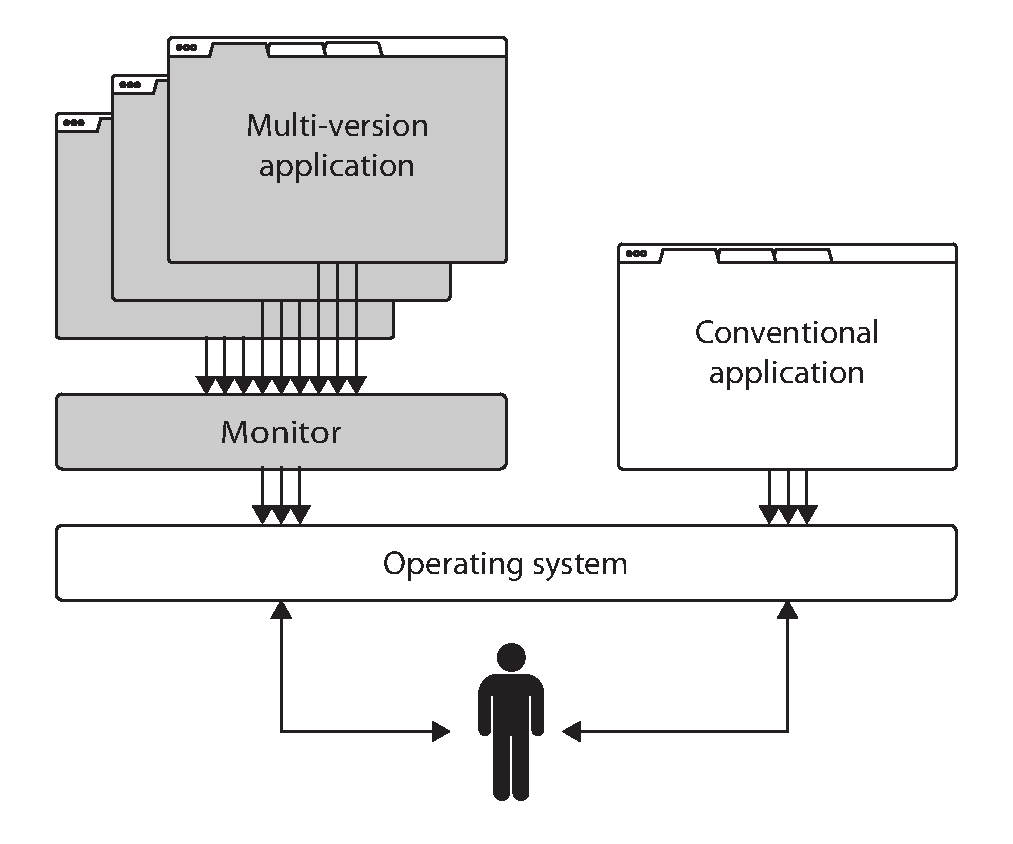
\includegraphics[width=0.5\textwidth]{multi-version/figures/platform}
    \caption{A platform running conventional and multi-version
      applications side by side.}
    \label{fig:mx-platform}
  \end{center}
\end{figure}

One particular challenge for our approach is to detect any divergences between
different software versions, resolve them in such a way as to increase the
overall reliability of the application, and finally synchronize again the
different versions after their executions reconverge to the same behavior.  Of
course, we also need to handle the case in which the executions of different
versions fail to reconverge to the same behavior after sufficient time.

Selecting the ``correct'' behavior of an application when different versions
disagree is of course not possible in the general case without having access to
a high-level specification.  However, one could%
\begin{inparaenum}[(1)]
\item focus on universal
correctness properties, such as the absence of crashes, and
\item use various
heuristics such as majority voting and favoring the latest application
versions.
\end{inparaenum}
Our approach is to resolve a divergence by always using the behavior of the
version that has not crashed, and favoring the behavior of the latest version
in all other cases. In this way, we ensure that the overall application has
strictly fewer crashes than any of the individual versions, while still using
the new security and bug fixes implemented in the latest version.

% Note that one key aspect on which our approach relies is
% \textit{having the different versions be alive at all times}.  This ensures
% that applications can survive crashes that occur at different points
% in different versions, but adds the extra challenge of restarting
% crashed versions.

%% Once divergences are detected, we need to decide what output should be
%% selected as the output of the multi-version system in order to improve
%% overall reliability.  Many different strategies can be used, but the
%% common goal is to ensure that the multi-version system will have
%% strictly fewer errors than any of the individual versions.

% Finally, our approach needs a deployment strategy to decide what versions are
% run in parallel when the number of available resources (\eg, idle CPU cores) is
% limited.  We envision several options---such as keeping the last $N$ released
% versions (where $N$ is the number of available resources), or keeping several
% very old stable versions---but the exact strategy should be decided on a
% case-by-case basis. % using existing empirical data.

\section{Challenges}

There are several different ways to implement an effective system call monitor,
each with its own set of trade-offs. The solutions targeting binaries are
significantly easier to use---they can be typically applied to off-the-shelf
binaries---but compared to solutions operating at source code level, they give
up some of the precision while typically require more engineering effort. The
most common ways for implementing monitors operating on binaries are dynamic
linking, \ptrace, kernel extensions and binary instrumentation, while solutions
targeting source code typically rely on source code instrumentation.

System calls are rarely performed directly by the application, which rather use
the wrapper functions provided by the C library. By linking to a custom
library, which provides a custom version of these functions, we could intercept
system calls performed by the application. This could be done either statically
at link time~\cite{plash}, or dynamically at runtime~\cite{shepherding:pldi14}
(\eg using \lstinline`LD_PRELOAD` or \lstinline`DYLD_INSERT_LIBRARIES`
variables). The major benefit of this approach is efficiency and relative ease
of implementation. However, the mechanism could be easily bypassed (\eg by
invoking system calls directly); also the C library ABI is has significantly
larger surface compared to the system call interface, requiring more
engineering effort.

\ptrace is an interface provided by most UNIX-like operating systems, including
Linux, providing means by which a process might observe and control another
process. The primary use of \ptrace interface is for debugging, but the
relative ease of use makes \ptrace a popular choice for implementing system
system call monitors~\cite{wily-hacker,orchestra09,tachyon12}. \ptrace-based
solutions require relatively low engineering effort, which makes them
especially suitable for rapid prototyping~\cite{spillane07}, they are easy to
deploy and fairly flexible. On the other hand, the use of \ptrace has numerous
drawbacks: a significant performance overhead due to large number of context
switches, problematic support for multi-threaded applications, and the lack of
filtering mechanism allowing interception only of system calls of interest.
\ptrace-based solution are also more difficult to debug as the use of \ptrace
disallows the use of \ptrace-based debuggers such as \gdb.

% The performance overhead could be partially improved by the use of
% more efficient mechanism for copying memory from/to the monitored process, such
% as shared memory as in case of Orchestra~\cite{orchestra09}, or cross memory
% attach as in case of \mx (\S\ref{sec:mxm}). The lack of filtering mechanism
% could be addressed by combining \ptrace with \textsf{seccomp/bpf} mechanism as
% shown by \textsc{Mbox}~\cite{mbox}.

An alternative to \ptrace is to implement the system call monitor
entirely~\cite{provos2002,cox2006} or partially in kernel space~\cite{ostia}.
While this approach has numerous advantages compared to other approaches, such
as minimal performance overhead and direct access to the application's
execution context and address space, there are several drawbacks.  First, this
approach requires kernel patches and/or new new kernel modules which
complicates the development, limits portability across different operating
systems or even different kernel versions, and hinders maintainability. Second,
the monitor must be run in privileged mode, which means that bugs in the
implementation may compromise the system stability. Furthermore, it also makes
it difficult for regular users to deploy and use such monitors.

Binary rewriting technique allow transforming the executable (either statically
or dynamically) altering its functionality; as such, it can be used to
implement system call monitor by rewriting all system call instructions into a
control flow transfer instructions (\eg a
\lstinline[language={[x64]Assembler}]`jmp` instruction). Existing monitors were
built either on top of existing binary rewriting
systems~\cite{onlinevalidation}, or using a purpose built binary translation
mechanism~\cite{vx32}. The advantage of binary rewriting-based monitors is
relatively low performance overhead, especially in the case of purpose built
rewriting mechanism. The main disadvantage is the complexity of implementation
which requires significant development effort.

In this thesis, we present two different designs for building monitors suitable
for multi-version execution. The first one, called \varan described in
Chapter~\ref{chap:efficient-execution}, is aimed towards running large number
of versions side-by-side with low performance overhead, and uses selective
binary rewriting to achieve this goal. The second one, called \mx described in
Chapter~\ref{chap:safe-updates}, is focused on surviving crashes caused by bugs
introduced in software updates, with the prototype implementation built using
the \ptrace mechanism.

%%%%%%%%%%%%%%%%%%%%%%%%%%%%%%%%%%%%%%%%%%%%%%%%%%%%%%%%%%%%%%%%%%%%%%%%%%%%%%

% Our approach aims to provide users with a third choice; when a new version
% arrives, instead of replacing the old version, we run both versions in
% parallel. In our example, consider that we are using \mx to run a
% version of \lighttpd from March 2009.  When the buggy April 2010 version
% is released, \mx runs it in parallel with the old one.  As the two
% versions execute:

% \begin{itemize}
% \item As long as the two versions have the same external behaviour (\eg they
%   write the same values into the same files, or send the same data over the
%   network), they are run side-by-side and \mx ensures that they act as one to
%   the outside world;

% \item When one of the versions crashes (\eg the new version executes the buggy
%   patch), \mx will patch the crashing version at runtime using the behaviour of
%   the non-crashing version.  In this way, \mx can successfully survive crash
%   bugs in both the old and the new version, increasing the reliability and
%   availability of the overall application;

% \item When a non-crashing divergence is detected, \mx will discard one of the
%   versions (by default the old one, but other heuristics can be used).  The
%   other version can be later restarted at a convenient synchronisation point
%   (\eg at the beginning of the dispatch loop of a network server).
% \end{itemize}

% To enable these scenarios, a monitor process coordinates the parallel execution
% of these variants\footnote{The terms \textit{version} and \textit{variant} are
% used interchangeably.} and synchronises their execution, making them appear as
% a single application to any outside entities.  While synchronisation can be
% performed at different levels, the most common approach is to do it at the
% level of system calls, for two main reasons: first, many existing
% diversification transformations, such as address-space layout
% randomisation~\cite{diehard06} and instruction-set
% randomisation~\cite{instr-set-rand03} do not change the sequence of system
% calls (the program's \textit{external behaviour}), and the ordering is often
% preserved even across different software versions.  Second, system
% calls are the main way in which the application communicates with the outside
% environment, and therefore
% %% the ultimate target of attackers.  Finally, as the main
% %% communication mechanism between applications and the environment,
% %% system calls
% must be virtualised in order to enable the multiple versions to act as
% one to the outside world.

\chapter{Software Evolution in Real-world}
\label{chap:evolution}

The multi-version execution approach is based on two key assumptions.  First,
that new bugs are being introduced during software evolution and maintenance
process even to a well tested code. Second, that during software evolution,
the externally observable behaviour of the applications remains relatively
stable, especially between minor revisions (\ie security and bug fixes).  While
there is a lot of first hand and anecdotal evidence in support of these
assumptions, despite the key role that software evolution plays in the
application life cycle, it is surprising how few empirical studies one can find
in the research literature regarding the evolution of the \emph{execution} of
real systems.

Software repositories provide rich information about the construction and
evolution of software systems. While static data extracted from software
repositories have been extensively studied, dynamic metrics concerning the
execution of the software have received much less attention, due to the
inherent difficulty of running and monitoring a large number of software
versions.

In this chapter, we present an empirical study concerning dynamic metrics which
aims to answer some of the questions related to software evolution. To perform
this study, we have built a flexible infrastructure that can be used to run
each version of a system in isolation and collect static and dynamic software
metrics from the test suite execution. We consider the tests to be an
(imperfect) proxy for a real-world execution.

%, using a lightweight virtualization environment based on software
%containers, that can be deployed on a cluster of local or cloud machines.

We have used this infrastructure to examine how code and tests co-evolve in
\numSystems popular open-source systems. We report the main characteristics of
software patches, analyse the evolution of program and patch coverage, assess
the impact of non-determinism on the execution of test suites, and investigate
whether the coverage of code containing bugs and bug fixes is higher than
average.

% While static metrics can provide useful insights into the construction and
% evolution of software, there are many software engineering aspects which
% require information about software executions.  For example, the research
% community has invested a lot of effort in designing techniques for improving
% the testing of software patches, ranging from test suite prioritisation and
% selection
% algorithms~\cite{harrold:test-redundancy,test-pri,Rothermel96analyzingregression}
% to program analysis techniques for test case generation and bug
% finding~\cite{diff-symex,directed-test-augmen:09,express,directed-symex11,babic11,directed-incr-symex11,patch:spin12,interaction-changes13}.

% Many of these techniques depend on the existence of a manual test suite,
% sometimes requiring the availability of a test exercising the
% patch~\cite{onlinevalidation,tachyon12}, sometimes making assumptions about the
% stability of program coverage or external behaviour over
% time~\cite{cov_regr97,mx}, other times using it as a starting point for
% exploration~\cite{zesti,pretex,sage,test-augmentation:genetic-vs-concolic}, and
% often times employing it as a baseline for
% comparison~\cite{klee,dotnet-random-test08,semantic-fp-testing12,mutation-tests-oracle12}.
% However, despite the key role that test suites play in software testing, it is
% surprising how few empirical studies one can find in the research literature
% regarding the co-evolution of test suites and code and their impact on the
% \emph{execution} of real systems.

% In this chapter, we present \covrig, a flexible infrastructure that can be used
% to run each version of a system in isolation and collect static and dynamic
% software metrics, using a lightweight virtual machine environment that can be
% deployed on a cluster of local or cloud machines.

% We use \covrig to conduct an empirical study examining how code and tests
% co-evolve in \numSystems popular open-source systems.  We report the main
% characteristics of software patches, analyse the evolution of program and patch
% coverage, assess the impact of non-determinism on the execution of test suites,
% and investigate whether the coverage of code containing bugs and bug fixes is
% higher than average.

% We use \covrig to conduct an empirical study examining how programs evolve in
% terms of code, tests and coverage.  More precisely, we have analysed the
% evolution of \numSystems popular software systems with a rich development
% history over a combined period of \numYears years, with the goal of answering
% the following list of research questions (RQs):

% \begin{itemize}
% \item[\textssc{RQ1}] \textit{\rqone}
%             Are coding and testing continuous, closely linked
%             activities?  Or do periods of intense development
%             alternate with periods of testing?

% \item[\textssc{RQ2}] \textit{\rqtwo}
%             Are most code
%             patches accompanied by a new or modified test case?  How
%             many patches modify neither executable code nor tests?
           
% \item[\textssc{RQ3}] \textit{\rqthree}
%             Are most patches small?  
%             How many different parts of the code does a patch touch?
%             What is the median number of lines, hunks and
%             files affected by a patch?

% \item[\textssc{RQ4}] \textit{\rqfour}  Do tests fail non-deterministically?
%             Does running the test suite multiple times cover different
%             lines of code?

% \item[\textssc{RQ5}] \textit{\rqfive}
%             Does the overall coverage increase steadily over time, or
%             does it remain constant?  Are there revisions that
%             significantly increase or decrease coverage?

% \item[\textssc{RQ6}] \textit{\rqsix}
%             What fraction of a patch is covered by the regression test
%             suite?  Does patch coverage depend on the size of the
%             patch?

% \item[\textssc{RQ7}] \textit{\rqseven}  Are
%             tests exercising recent patches added shortly after the
%             patch was submitted?  If so, how significant is this
%             latent patch coverage?

% \item[\textssc{RQ8}] \textit{\rqeight}
%             Are most fixes thoroughly exercised by the regression
%             suite?  How many fixes are entirely executed?

% \item[\textssc{RQ9}] \textit{\rqnine}
%             Is code that contains bugs exercised less than other changes?
%             Is coverage a reasonable indicator of code quality? 

% %\item[\bf RQ10:] \textbf{Does buggy code have lower than average coverage?}
% \end{itemize}

\begin{figure}[t!]
\centering
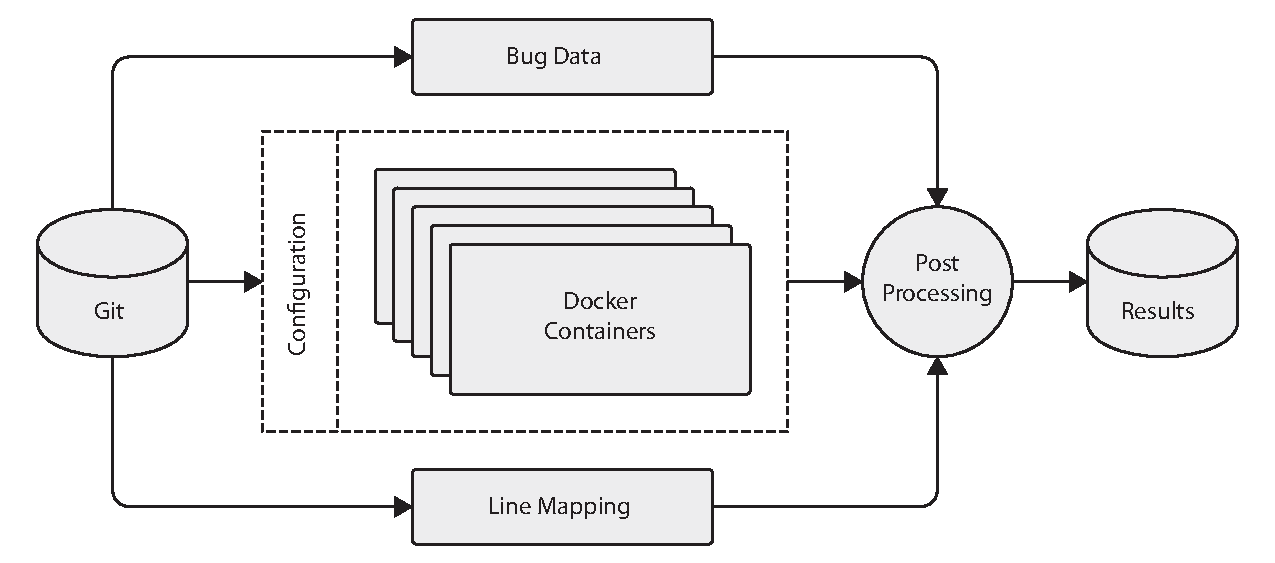
\includegraphics[width=\columnwidth]{evolution/figures/pipeline}
\caption{\covrig infrastructure.}
\label{fig:arch}
\end{figure}

The overall architecture of the \covrig infrastructure is depicted
in Figure~\ref{fig:arch}.  It contains a generic driver which
iterates through all the revisions in a given range and invokes
routines specific to each system to compile, run, and collect
statistics of interest.

%% To collect information about each program revision, such as whether it
%% successfully compiles, whether it passes the regression tests and with
%% what coverage, we built an infrastructure capable of automatically
%% retrieving and compiling each version of a target program, running
%% existing regression tests and collecting metrics of interest.

%The system is built on top of software containers~\cite{}, a
%lightweight virtualisation mechanism, which offers both isolation and
%reproducibility, by ensuring a consistent environment into which to
%run each software revision.  In this way, the execution of different
%revisions do not influence each other, \eg by inadvertently leaving
%behind lock files or not properly freeing up resources.

\paragraph{Lightweight software containers} \covrig employs software
containers~\cite{containers:eurosys07}, an operating system-level
virtualisation mechanism that provides the ability to run multiple
isolated virtual Linux systems (``containers'') inside a single host
OS.  When launched, \covrig starts by loading the selected range of
revisions from the project's \git repository, and for each revision
starts a new software container.  The use of containers offers
increased isolation and reproducibility guarantees by providing a
consistent environment in which to run each software revision and
ensuring that different revisions do not interfere with each other,
\eg by inadvertently leaving behind lock files or not properly freeing
up resources.

The choice of lightweight OS-level virtualisation rather than more
traditional virtual machines (\eg
\kvm\footnote{\url{http://www.linux-kvm.org/}} or
\xen\footnote{\url{http://www.xenproject.org/}}) reduces the
performance penalty associated with spawning and tearing down VMs,
operations performed for each revision analysed.  To get a sense of
this difference, we compared an
\lxc\footnote{\url{http://linuxcontainers.org/}} container, which
required under a second for these operations, with a \xen VM, which
needed over a minute.

In our implementation, we use
\docker\footnote{\url{https://www.docker.io/}} to create and manage
the lower-level \lxc containers, and
%Vagrant to
deploy them on multiple local or cloud machines.
Each container is used to configure, compile and test one
program revision, as well as collect the metrics of interest, such as
code size and coverage. The containers are remotely controlled through
SSH using the \fabric\footnote{\url{http://fabfile.org/}} framework.


\paragraph{Configuration file} \covrig has a modular architecture, which makes it
possible to analyse new systems with modest effort. A potential user
of our infrastructure only needs to provide a Python
configuration file describing the system.  A minimal file provides
the name of the system, its \git repository location, a method to
compile the system, \eg install dependencies and run the appropriate
\stt{make} command, and a method to run the regression tests, \eg run
the \stt{make test} command.
%
Finally, the configuration file can also specify an {\em end revision}
and a specific number of revisions to analyse.  
%% \covrig will use these parameters to determine the list of revisions to
%% analyse, independent of the target system's evolution.  
For accurate test suite size measurements, the files or folders which
make up the test suite can also be indicated.

For each revision, \covrig collects several static and dynamic metrics.  The
static metrics are obtained either directly from the version control
system (\eg the number of lines of test code) or after compiling each
revision (\eg the number of executable lines of code).  The dynamic
metrics require running the regression tests (\eg the overall line
coverage or the regression test success status).

Further information and graphs---including the ones presented in our
empirical study---are automatically derived in the post-processing
stage from these primary metrics using a set of scripts.

%% For example, we were able to verify that the {\em latent patch
%% coverage}, \ie the fraction of code which is executed only several
%% revisions after it is introduced is small, and practitioners can
%% safely ignore it most of the time when evaluating test suite
%% augmentation or coverage-improvement techniques.


%\subsection{Bug Data} \label{ssec:bugdesign}

\paragraph{Bug data} One possible application of \covrig is finding
useful data about software bugs and correlating them with the static
and dynamic metrics collected. For our study, we mined bug data from
both software repositories and, where available, bug tracking systems.
We automatically obtained a list of candidate bug-fixing revisions by
iterating through the list of commits and checking the commit message
for words such as {\em fix}, {\em bug} or {\em issue}, followed by a
number representing the bug identifier.  For example, a typical
\memcached bug fix commit message looks like {\em "Issue 224 - check
  retval of main event loop"}. The regular expression that we used to
identify these commits is similar to the ones used in prior
work~\cite{genealogies:issre13}:

\lstinline`(?:bug|issue|fix|resolve|close)\s*\#?\s?(\d+)`

Where possible, we confirmed that the bug identifier is valid by
querying the associated bug tracking system. We further manually
checked all reported revisions and confirmed that they included no
false positives.  While it is impossible to quantify the false
negative rate without a knowledgeable developer manually checking all
the revisions in a repository, we believe that the automatically
obtained bug fixes create a representative subset of the fixes in the
repository.

\paragraph{Line mapping} The ability to track how lines move and change
across revisions is the cornerstone of many high-level software
evolution analyses.  A line mapping algorithm improves over the
traditional \diff algorithm by tracking the movement of individual
lines rather than hunks.  Conceptually, line mapping is a function
which takes two revisions, \textit{r1} and \textit{r2}, and a program
location described by a pair \textit{(file name 1, line number 1)}
associated with \textit{r1}.  The output is a pair \textit{(file name
  2, line number 2)} identifying the corresponding location in
\textit{r2}.

Our implementation of the line mapping algorithm is similar to the
algorithms described in previous
work~\cite{szz:msr05,szz:ase06,change-source-code:msr07,szzrevisited:defects08}.
It makes use of the \emph{Levenshtein edit
  distance}~\cite{levenshtein1966binary} to track line edits, and
\emph{tf--idf}~\cite{tf-idf} and \emph{cosine
  similarity}~\cite{cosinesimilarity} to track line movements.  It
also uses the \emph{Hungarian algorithm}~\cite{hungarian} to find the
optimal matching of lines across versions.  Compared to previous work,
our implementation can also improve precision by using coverage information to filter
non-executable lines.

%% We used line mapping in two ways in our analysis: to determine whether
%% patches are tested within the next few revisions after they were
%% created (\S\ref{sec:lpcoverage}), and to estimate where bugs were
%% introduced (\S\ref{sec:bugs}).

In our study, we used line mapping to determine whether patches are
tested within the next few revisions after they were created
(\S\ref{sec:lpcoverage}).

\paragraph{Cloud deployment} To enable large-scale data collection and
processing, we deployed \covrig to our private cloud.  We have built our
system around a standard set of tools: Packer for building custom
Docker-enabled machine images, Vagrant for controlling and provisioning
the virtual machines based on these images, a Docker registry for
serving \covrig's Docker containers and a {\em fabfile} for
orchestrating the entire cluster. The same set of tools and scripts
can be used to deploy \covrig to different private or public clouds.

%% \subsection{High-Level Questions} \label{ssec:highlevel}

%% Coverage, bugs and line mapping data already provide useful insights into a
%% software project. For example, coverage and known bugs count can be used to
%% predict the residual bugs, i.e., the bugs still present in the software, using
%% a simple formula~\cite{coveragedefects98}

%% Using the bug data, we can quantify the number of patches which attempt to fix
%% a bug but either contain an incomplete fix or introduce new bugs. Such patches
%% are identified by looking for bug pairs, one being fixed and the other
%% introduced in the same patch. A high number of buggy fixes points to
%% deficiencies in the software development process.

%% \todo{More interesting things that we can do directly with coverage, bugs and
%% line mapping data}

%% However, further processing of this data allows us to answer more questions.
%% Combining  bug data and coverage data allows us to determine how many bugs are
%% in code which was already tested, i.e. executed without triggering the bug.
%% This may happen because the bug is only activated in corner-case scenarios.
%% Systems with a high number of bugs present in tested code may benefit from
%% symbolic execution-based testing tools such as ZESTI~\cite{zesti}, which
%% transparently instrument the existing tests to check for corner-case scenarios.
%% On the other hand, systems where the bugs are present in untested code can
%% benefit from test generation tools such as KATCH~\cite{katch}.

%% Correlations between bug data and software metrics can be used to build a bug
%% predictors based on project history and current patch coverage. Integrated in a
%% development environment or continuous integration system, such predictors can
%% warn developers when making high-risk changes. An intuitive predictor is based
%% on patch coverage: a tested patch is less likely to be buggy, compared to an
%% untested patch and the correlation can be mined from the project history. Code
%% churn can also be used as a predictor~\cite{churn-bugs:issre96, churndefects05}
%% and can be further refined to by eliminating non-executable changes or using
%% fine-grained souce code change extraction techniques~\cite{fluri:scc}
%% and its relationship with bugs can be mined using the line mapping data at the
%% line/function/file level.
%% % But we really don't want to go too much into statistics

%% Another question is whether old regression tests are still adequate for the
%% latest program version. We can quantify test adequacy by the fraction of the
%% code originally executed by the test that is still executed in the current
%% version. For an accurate computation we need to map the lines originally
%% executed to their counterparts in the current version.

\section{Overview}
\label{evolution:overview}

We used the our infrastructure to understand the evolution of \numSystems
popular open-source applications written in C/C++, over a combined period of
\numYears years. The \numSystems evaluated applications are:

\begin{enumerate}

\item[\gnu~\binutils\footnote{\url{http://www.gnu.org/software/binutils/}}]
is a set of utilities for inspecting and modifying object files,
libraries and binary programs.  We selected for analysis the twelve
utilities from the \stt{binutils} folder (\stt{addr2line}, \stt{ar},
\stt{cxxfilt}, \stt{elfedit}, \stt{nm}, \stt{objcopy}, \stt{objdump},
\stt{ranlib}, \stt{readelf}, \stt{size}, \stt{strings} and \stt{strip}),
which are standard user-level programs under many UNIX distributions.

\item[\beanstalkd\footnote{\url{http://kr.github.io/beanstalkd/}}]
is a simple and fast work queue originally designed for reducing the latency of
page views in high-volume web applications.

\item[\git\footnote{\url{http://git-scm.com/}}]
is one the most popular distributed version control systems used by the
open-source developer community.

\item[\lighttpd\footnote{\url{http://www.lighttpd.net/}}]
is a lightweight web server optimized for high performance environments.

\item[\lighttpdtwo\footnote{\url{http://redmine.lighttpdtwo.net/projects/lighttpdtwo2/}}]
is the new major version of the \lighttpd web server developed entirely from
scratch by the same team of developers.

\item[\memcached\footnote{\url{http://memcached.org/}}]
is a general-purpose distributed memory caching system used by several popular
sites such as Craigslist, Digg and Twitter.

\item[\redis\footnote{\url{http://redis.io/}}]
is a popular key-value data store used by many well-known services such as
Twitter, GitHub and StackOverflow.

\item[\vim\footnote{\url{http://www.vim.org/}}] is arguably one of the most
popular text editors.

\item[\zeromq\footnote{\url{http://zeromq.org/}}]
is a high-performance asynchronous messaging middleware library used by a
number of organisations such as Los Alamos Labs, NASA and CERN.

%\item {\bf GNU diffutils} is a collection of four widely-used
%programs: \stt{diff}, \stt{sdiff}, \stt{diff3} and \stt{cmp}, part of
%many popular UNIX distributions.

\end{enumerate}

The \numSystems applications are representative for C/C++ open-source code: GNU
\binutils are user-level utilities, \git is a version control system,
\beanstalkd, \lighttpdtwo, \memcached and \redis are server applications, \vim
is a text editor while \zeromq is a library.  All applications include a
regression test suite.

\begin{table}[t]
\caption{Summary of applications used in our study.
\textit{ELOC} represents the number of executable lines of code and
\textit{TLOC} the number of lines in test files in the last revision
analysed.}
\begin{center}
\begin{tabular}{llrlr}
\toprule
\multicolumn{1}{c}{}     & \multicolumn{2}{c}{\sc Code}& \multicolumn{2}{c}{\sc Tests} \\
\cmidrule(r){2-3}\cmidrule(l){4-5}
\textsc{Application} & \textsc{Language} & \textsc{ELOC} & \textsc{Language} & \textsc{TLOC}          % & \bf Time         
\\ \midrule
\beanstalkd  & C         & \beanstalkdSize & C        & \beanstalkdTsize  % & \beanstalkdTestTime
\\
\binutils    & C         & \binutilsSize  & DejaGnu   & \binutilsTsize    % & \binutilsTestTime 
\\
\git         & C         & \gitSize       & C/shell   & \gitTsize         % & \gitTestTime 
\\
\lighttpd    & C         & \lighttpdSize  & Perl    & \lighttpdTsize    % & \lighttpdtwoTestTime 
\\
\lighttpdtwo    & C         & \lighttpdtwoSize  & Python    & \lighttpdtwoTsize    % & \lighttpdtwoTestTime 
\\
\memcached   & C         & \memcachedSize & C/Perl    & \memcachedTsize   % & \memcachedTestTime 
\\
\redis       & C         & \redisSize     & Tcl       & \redisTsize       % & \redisTestTime    
\\
\vim         & C         & \vimSize       & Vim script       & \vimTsize      % & \vimTestTime   
\\
\zeromq      & C++       & \zeromqSize    & C++       & \zeromqTsize      % & \zeromqTestTime   
\\ \bottomrule
\end{tabular}
\end{center}
\label{tbl:study-systems}
\end{table}

\subsection{Basic characteristics}

Table~\ref{tbl:study-systems} shows some basic characteristics of these
systems: the language in which the code and tests are written, the number of
executable lines of code (ELOC) and the number of lines of test code (TLOC) in
the last revision analysed. To accurately measure the number of ELOC, we
leveraged the information stored by the compiler in \texttt{gcov} graph files,
while to measure the number of TLOC we did a simple line count of the test
files (using \texttt{cloc}, or \texttt{wc~-l} when \texttt{cloc} cannot detect
the file types).

The code size for these applications varies from only \memcachedSize ELOC for
\memcached to \gitSize ELOC for \git.  The test code is written in a variety of
languages and ranges from \lighttpdtwoTsize lines of Python code for
\lighttpdtwo to \gitTsize lines of C and shell code for \git.  The test code is
36\% larger than the application code in the case of \git, approximately as
large as the application code for \memcached, around 40\% of the application
code for \redis and \zeromq, and only around 10\% and 19\% of the application
code for \lighttpdtwo, \vim and \binutils respectively.  Running the test suite
on the last version takes only a few seconds for \binutils, \lighttpdtwo, \vim
and \zeromq, \memcachedTestTime seconds for \memcached, \redisTestTime seconds
for \redis, and 30 minutes for \git, using a four-core Intel Xeon E3-1280
machine with 16 GB of RAM.

The version control system used by majority of these applications is \git.
Four of these projects---\git, \memcached, \redis, and \zeromq ---are hosted on
the \github\footnote{\url{https://github.com/}} online project site.  The other
two---\binutils and \lighttpdtwo---use their own \git hosting. \lighttpd uses
Subversion, but the project also provides a \git mirror on \github. \vim uses
Mercurial.

\subsection{Selection of revisions}

Our goal was to select a comparable number of revisions across applications.
The methodology was to start from the current version at the day of our
experiments, and select an equal number of previous revisions for all systems.
We only counted revisions which modify executable code, tests or both because
this is what our analyses look at. We decided to select 250 such revisions from
each system because some systems had non-trivial dependency issues further back
than this, which prevented us from properly compiling or running them.  We
still had to install the correct dependencies where appropriate, \eg downgrade
\stt{libev} for older versions of \lighttpdtwo and \stt{libevent} for
\memcached.

Note that not all revisions compile, either due to development errors
%(an example of this would be someone forgetting to add a file) 
or portability issues (\eg system header files differing across OS
distributions).
%% Note that we distinguish between this kind of permanent errors (which
%% disallow us to compile all versions earlier than some revision) and
%% more transient compilation errors that affect only some program
%% versions.  
Redis has the largest number of such transient compilation
errors---\redisTransientCompErrs.  The prevailing reasons are missing
\stt{\#include} directives, \eg \stt{unistd.h} for the \stt{sleep} function,
and compiler warnings subsequently treated as errors.  The missing
\stt{\#include} directives most likely slipped past the developers because on
some systems other \stt{libc} headers cause the missing headers to be
indirectly included. The compiler warnings were generated because newer
compiler versions, such as the one that we used, are more pedantic.  Other
reasons include forgotten files and even missing semicolons.

We decided to fix the errors which had likely not been seen at the time a
particular revision was created, for example by adding the compile flag
\stt{-Wno-error} in \binutils so that warnings do not terminate the build
process. In all situations when we could not compile a revision, we rolled over
the changes to the next revisions until we found one where compilation was
successful.  Revisions which do not successfully compile are not counted
towards the 250 limit.

Another important decision concerns the granularity of the revisions
being considered.  Modern decentralised software repositories based on
version control systems such as \git do not have a linear structure
and the development history is a directed acyclic graph rather than a
simple chain.  Different development styles generate different
development histories; for example, \git, \redis and \zeromq exhibit a
large amount of branching and merging while the other three systems
have a mostly linear history.  Our decision was to focus on the main branch,
and treat each merge into it as a single revision. In other words, we
considered each feature branch a single indivisible unit.  Our
motivation for this decision was twofold: first, development branches
are often spawned by individual developers in order to work on a
certain issue and are often ``private'' until they are merged into the
main branch.  As a result, sub-revisions in such branches are often
unusable or even non-compilable, reflecting work-in-progress.  Second,
the main branch is generally the one tracked by most users, therefore
analysing revisions at this level is a good match in terms of
understanding what problems are seen in the field.  This being said,
there are certainly development styles and research questions that would
require tracking additional branches; however, we believe that for our
benchmarks and research questions this level of granularity provides meaningful
answers.

% On a secondary note, we remark that an additional complication with
% this approach is that version control systems do not associate a
% branch name to each revision, so some detective work might be required
% to follow the main development branch.  However, since
% the projects exhibiting a branching structure are hosted on \github, an implicit central
% integrator exists (the project owner) and we considered their history
% to be the official one, essentially always following the first parent
% in a merge.

\begin{table}[t]
\centering
\caption{Revisions used in our study.
  {\em OK}:~code compiles and tests complete successfully,
  {\em TF}:~some tests fail,
  {\em TO}:~tests time out,
  {\em CF}:~compilation fails,
  {\em Time}:~the number of months analysed.}
\begin{tabular}{lrrrrr}
\toprule
\multicolumn{1}{c}{}          &       \multicolumn{3}{c}{\sc OK+TF+TO=250}                 &            \multicolumn{2}{c}{}                   \\
\cmidrule{2-4}
\textsc{Application} & \textsc{OK} & \textsc{TF} & \textsc{TO} & \textsc{CF} & \textsc{Time}           \\
\midrule
\beanstalkd  &  \beanstalkdOK & \beanstalkdTransientTestErrs & \beanstalkdTransientTestTimeouts & \beanstalkdTransientCompErrs  &  {\beanstalkdTimespan}mo \\
\binutils    &  \binutilsOK   & \binutilsTransientTestErrs  & \binutilsTransientTestTimeouts  & \binutilsTransientCompErrs  &  {\binutilsTimespan}mo \\
\git         &  \gitOK        & \gitTransientTestErrs       & \gitTransientTestTimeouts       & \gitTransientCompErrs       &  {\gitTimespan}mo  \\
\lighttpd    &  \lighttpdOK   & \lighttpdTransientTestErrs  & \lighttpdTransientTestTimeouts  & \lighttpdTransientCompErrs  &  {\lighttpdTimespan}mo  \\
\lighttpdtwo    &  \lighttpdtwoOK   & \lighttpdtwoTransientTestErrs  & \lighttpdtwoTransientTestTimeouts  & \lighttpdtwoTransientCompErrs  &  {\lighttpdtwoTimespan}mo  \\
\memcached   &  \memcachedOK  & \memcachedTransientTestErrs & \memcachedTransientTestTimeouts & \memcachedTransientCompErrs &  {\memcachedTimespan}mo \\
\redis       &  \redisOK      & \redisTransientTestErrs     & \redisTransientTestTimeouts     & \redisTransientCompErrs     &  {\redisTimespan}mo     \\
\vim         &  \vimOK        & \vimTransientTestErrs       & \vimTransientTestTimeouts       & \vimTransientCompErrs    &  {\vimTimespan}mo    \\
\zeromq      &  \zeromqOK     & \zeromqTransientTestErrs    & \zeromqTransientTestTimeouts    & \zeromqTransientCompErrs    &  {\zeromqTimespan}mo    \\
\bottomrule
\end{tabular}
\label{tbl:revisions}
\end{table}


Table~\ref{tbl:revisions} summarises the revisions that we selected:
they are grouped into those that compile and pass all the tests (\emph{OK}),
compile but fail some tests (\emph{TF}), compile but time out while running the
test suite (\emph{TO}), and fail to compile (\emph{CF}).  The time limit that
we enforced was empirically selected for each system such that it is large
enough to allow a correct revision to complete all tests. As shown in the
table, timeouts were a rare occurrence, with at most one occurrence per
application.

Table~\ref{tbl:revisions} also shows the development time span
considered, which ranges from only 5-6 months for \git and \redis,
which had a fast-paced development during this period, to almost 4
years for \memcached. The age of the projects at the first version
that we analysed ranges from a little over 2 years for \lighttpdtwo,
to 11 years for \binutils.
%6 years memcached, 4 years redis, 2yr 9mo zeromq, 8 years git

\subsection{Revision setup}

All the programs analysed were compiled to record coverage information. In
addition, we disabled compiler optimisations, which generally interact poorly
with coverage measurements. We used existing build targets and configuration
options if available, otherwise we configured the application with the flags
\lstinline`CFLAGS='-O0 -coverage'` and \lstinline`LDFLAGS=-coverage`. All code
from the system headers, \ie \stt{/usr/include/} was excluded from the results.

Each revision was run in a virtualised environment based on 64-bit version of
Ubuntu 12.10 (12.04.3 for \git) running inside an \lxc container.  To take
advantage of the inherent parallelism of this approach, the containers were
spawned in one of 28 long-running \xen VMs, each with a 4~Ghz CPU, 6~GB of RAM,
and 20~GB of storage, running a 64-bit version of Ubuntu 12.04.3.

% The following sections present the main findings of our analysis.  They first
% reiterate and then examine in detail our target research questions (RQs).

We used the \covrig infrastructure to understand the evolution of
\numSystems popular open-source applications written in C/C++, over a
combined period of \numYears years. The six evaluated applications are:

\begin{enumerate}

\item[\gnu~\binutils\footnote{\url{http://www.gnu.org/software/binutils/}}]
is a set of utilities for inspecting and modifying object files,
libraries and binary programs.  We selected for analysis the twelve
utilities from the \stt{binutils} folder (\stt{addr2line}, \stt{ar},
\stt{cxxfilt}, \stt{elfedit}, \stt{nm}, \stt{objcopy}, \stt{objdump},
\stt{ranlib}, \stt{readelf}, \stt{size}, \stt{strings} and \stt{strip}),
which are standard user-level programs under many UNIX distributions.

\item[\beanstalkd\footnote{\url{http://kr.github.io/beanstalkd/}}] is a
  simple and fast work queue originally designed for reducing the latency of
  page views in high-volume web applications.

\item[\git\footnote{\url{http://git-scm.com/}}] is one the
most popular distributed version control systems used by the open-source
developer community.

\item[\lighttpdtwo\footnote{\url{http://redmine.lighttpdtwo.net/projects/lighttpdtwo2/}}]
is a lightweight web server optimized for high performance environments.
We examined version 2, which is the latest development branch.

\item[\memcached\footnote{\url{http://memcached.org/}}]
is a general-purpose distributed memory caching system used by several
popular sites such as Craigslist, Digg and Twitter.

\item[\redis\footnote{\url{http://redis.io/}}]
is a popular key-value data store used by many well-known
services such as Twitter, GitHub and StackOverflow.

\item[\zeromq\footnote{\url{http://zeromq.org/}}]
is a high-performance asynchronous messaging middleware library used by
a number of organisations such as Los Alamos Labs, NASA and CERN.

%\item {\bf GNU diffutils} is a collection of four widely-used
%programs: \stt{diff}, \stt{sdiff}, \stt{diff3} and \stt{cmp}, part of
%many popular UNIX distributions.

\end{enumerate}

The \numSystems applications are representative for C/C++ open-source
code: GNU \binutils are user-level utilities, \git is a version
control system, \beanstalkd, \lighttpdtwo, \memcached and \redis are server
applications, while \zeromq is a library.  All applications include a
regression test suite.

\begin{table}[t]
\caption{Summary of applications used in our study.
\textit{ELOC} represents the number of executable lines of code and
\textit{TLOC} the number of lines in test files in the last revision
analysed.}
\begin{center}
\begin{tabular}{llrlr}
\toprule
\multicolumn{1}{c}{}     & \multicolumn{2}{c}{\sc Code}& \multicolumn{2}{c}{\sc Tests} \\
\cmidrule(r){2-3}\cmidrule(l){4-5}
\textsc{Application} & \textsc{Language} & \textsc{ELOC} & \textsc{Language} & \textsc{TLOC}          % & \bf Time         
\\ \midrule
\beanstalkd  & C         & \beanstalkdSize & C        & \beanstalkdTsize  % & \beanstalkdTestTime
\\
\binutils    & C         & \binutilsSize  & DejaGnu   & \binutilsTsize    % & \binutilsTestTime 
\\
\git         & C         & \gitSize       & C/shell   & \gitTsize         % & \gitTestTime 
\\
\lighttpdtwo    & C         & \lighttpdtwoSize  & Python    & \lighttpdtwoTsize    % & \lighttpdtwoTestTime 
\\
\memcached   & C         & \memcachedSize & C/Perl    & \memcachedTsize   % & \memcachedTestTime 
\\
\redis       & C         & \redisSize     & Tcl       & \redisTsize       % & \redisTestTime    
\\
\zeromq      & C++       & \zeromqSize    & C++       & \zeromqTsize      % & \zeromqTestTime   
\\ \bottomrule
\end{tabular}
\end{center}
\label{tbl:systems}
\end{table}

\paragraph{Basic characteristics} Table~\ref{tbl:systems} shows some basic
characteristics of these systems: the language in which the code and tests are
written, the number of executable lines of code (ELOC) and the number of lines
of test code (TLOC) in the last revision analysed. To accurately measure the
number of ELOC, we leveraged the information stored by the compiler in
\texttt{gcov} graph files, while to measure the number of TLOC we did a simple
line count of the test files (using \texttt{cloc}, or \texttt{wc~-l} when
\texttt{cloc} cannot detect the file types).

The code size for these applications varies from only \memcachedSize
ELOC for \memcached to \gitSize ELOC for \git.  The test code is written in
a variety of languages and ranges from \lighttpdtwoTsize lines of Python
code for \lighttpdtwo to \gitTsize lines of C and shell code for \git.
The test code is 36\% larger than the application code in the case
of \git, approximately as large as the application code for
\memcached, around 40\% of the application code for \redis and \zeromq,
and only around 10\% and 19\% of the application code for \lighttpdtwo and
\binutils respectively.  Running the test suite on the last version 
takes only a few seconds for \binutils, \lighttpdtwo, and \zeromq,
\memcachedTestTime seconds for \memcached, \redisTestTime seconds for 
\redis, and 30 minutes for \git, using a four-core Intel Xeon 
E3-1280 machine with 16 GB of RAM.

The version control system used by all these applications is \git.  Four
of these projects---\git, \memcached, \redis, and \zeromq ---are hosted
on the \github\footnote{\url{https://github.com/}} online project site.
The other two---\binutils and \lighttpdtwo---use their own \git hosting.


\paragraph{Selection of revisions} Our goal was to select a comparable number
of revisions across applications. The methodology was to start from the current
version at the day of our experiments, and select an equal number of previous
revisions for all systems. We only counted revisions which modify executable
code, tests or both because this is what our analyses look at. We decided to
select 250 such revisions from each system because some systems had non-trivial
dependency issues further back than this, which prevented us from properly
compiling or running them.  We still had to install the correct dependencies
where appropriate, \eg downgrade \stt{libev} for older versions of \lighttpdtwo
and \stt{libevent} for \memcached.

Note that not all revisions compile, either due to development errors
%(an example of this would be someone forgetting to add a file) 
or portability issues (\eg system header files differing across OS
distributions).
%% Note that we distinguish between this kind of permanent errors (which
%% disallow us to compile all versions earlier than some revision) and
%% more transient compilation errors that affect only some program
%% versions.  
Redis has the largest number of such transient compilation
errors---\redisTransientCompErrs.  The prevailing reasons are
missing \stt{\#include} directives, \eg \stt{unistd.h} for
the \stt{sleep} function, and compiler warnings subsequently treated as errors.
The missing \stt{\#include} directives most likely slipped past the
developers because on some systems other \stt{libc} headers cause the
missing headers to be indirectly included. The compiler warnings were
generated because newer compiler versions, such as the one that we used,
are more pedantic.
Other reasons include forgotten files and even missing semicolons.

We decided to fix the errors which had likely not been seen at the
time a particular revision was created, for example by adding the
compile flag \stt{-Wno-error} in \binutils so that warnings do not
terminate the build process. In all situations when we could not
compile a revision, we rolled over the changes to the next revisions
until we found one where compilation was successful.  Revisions which
do not successfully compile are not counted towards the 250 limit.

Another important decision concerns the granularity of the revisions
being considered.  Modern decentralised software repositories based on
version control systems such as \git do not have a linear structure
and the development history is a directed acyclic graph rather than a
simple chain.  Different development styles generate different
development histories; for example, \git, \redis and \zeromq exhibit a
large amount of branching and merging while the other three systems
have a mostly linear history.  Our decision was to focus on the main branch,
and treat each merge into it as a single revision. In other words, we
considered each feature branch a single indivisible unit.  Our
motivation for this decision was twofold: first, development branches
are often spawned by individual developers in order to work on a
certain issue and are often ``private'' until they are merged into the
main branch.  As a result, sub-revisions in such branches are often
unusable or even non-compilable, reflecting work-in-progress.  Second,
the main branch is generally the one tracked by most users, therefore
analysing revisions at this level is a good match in terms of
understanding what problems are seen in the field.  This being said,
there are certainly development styles and/or research questions that
would require tracking additional branches; however, we believe that
for our benchmarks and research questions this level of granularity
provides meaningful answers.

% On a secondary note, we remark that an additional complication with
% this approach is that version control systems do not associate a
% branch name to each revision, so some detective work might be required
% to follow the main development branch.  However, since
% the projects exhibiting a branching structure are hosted on \github, an implicit central
% integrator exists (the project owner) and we considered their history
% to be the official one, essentially always following the first parent
% in a merge.


\begin{table}[t]
\centering
\caption{Revisions used in our study.
  {\em OK}:~code compiles and tests complete successfully,
  {\em TF}:~some tests fail,
  {\em TO}:~tests time out,
  {\em CF}:~compilation fails,
  {\em Time}:~the number of months analysed.}
\begin{tabular}{lrrrrr}
\toprule
\multicolumn{1}{c}{}          &       \multicolumn{3}{c}{\sc OK+TF+TO=250}                 &            \multicolumn{2}{c}{}                   \\
\cmidrule{2-4}
\textsc{Application} & \textsc{OK} & \textsc{TF} & \textsc{TO} & \textsc{CF} & \textsc{Time}           \\
\midrule
\beanstalkd  &  \beanstalkdOK & \beanstalkdTransientTestErrs & \beanstalkdTransientTestTimeouts & \beanstalkdTransientCompErrs  &  {\beanstalkdTimespan}mo \\
\binutils    &  \binutilsOK   & \binutilsTransientTestErrs  & \binutilsTransientTestTimeouts  & \binutilsTransientCompErrs  &  {\binutilsTimespan}mo \\
\git         &  \gitOK        & \gitTransientTestErrs       & \gitTransientTestTimeouts       & \gitTransientCompErrs       &  {\gitTimespan}mo  \\
\lighttpdtwo    &  \lighttpdtwoOK   & \lighttpdtwoTransientTestErrs  & \lighttpdtwoTransientTestTimeouts  & \lighttpdtwoTransientCompErrs  &  {\lighttpdtwoTimespan}mo  \\
\memcached   &  \memcachedOK  & \memcachedTransientTestErrs & \memcachedTransientTestTimeouts & \memcachedTransientCompErrs &  {\memcachedTimespan}mo \\
\redis       &  \redisOK      & \redisTransientTestErrs     & \redisTransientTestTimeouts     & \redisTransientCompErrs     &  {\redisTimespan}mo     \\
\zeromq      &  \zeromqOK     & \zeromqTransientTestErrs    & \zeromqTransientTestTimeouts    & \zeromqTransientCompErrs    &  {\zeromqTimespan}mo    \\
\bottomrule
\end{tabular}
\label{tbl:revisions}
\end{table}


Table~\ref{tbl:revisions} summarises the revisions that we selected:
they are grouped into those that compile and pass all the tests
(\textit{OK}), compile but fail some tests (\textit{TF}),
and compile but time out while running the test suite
(\textit{TO}).
The time limit that we enforced was empirically selected for
each system such that it is large enough to allow a correct revision
to complete all tests. As shown in the table, timeouts were a rare
occurrence, with at most one occurrence per application.

Table~\ref{tbl:revisions} also shows the development time span
considered, which ranges from only 5-6 months for \git and \redis,
which had a fast-paced development during this period, to almost 4
years for \memcached. The age of the projects at the first version
that we analysed ranges from a little over 2 years for \lighttpdtwo
(version 2), to 11 years for \binutils.
%6 years memcached, 4 years redis, 2yr 9mo zeromq, 8 years git

\paragraph{Setup} All the programs analysed were compiled to record coverage
information. In addition, we disabled compiler optimisations, which generally
interact poorly with coverage measurements. For this we used existing build
targets and configuration options if available, otherwise we configured the
application with the flags \lstinline`CFLAGS='-O0 -coverage'` and
\lstinline`LDFLAGS=-coverage`. All code from the system headers, \ie
\stt{/usr/include/} was excluded from the results.

Each revision was run in a virtualised environment based on 64-bit version of
Ubuntu 12.10 (12.04.3 for \git) running inside an \lxc container.  To take
advantage of the inherent parallelism of this approach, the containers were
spawned in one of 28 long-running \xen VMs, each with a 4~Ghz CPU, 6~GB of RAM,
and 20~GB of storage, running a 64-bit version of Ubuntu 12.04.3.

The following subsections present the main findings of our analysis.  They
first reiterate and then examine in detail our target research questions (RQs).

\subsection{Code and Test Evolution}

\begin{figure}[t]
%\input{evolution/graphs/eloc.tex}
\includegraphics[width=\textwidth]{evolution/graphs/eloc.pdf}
\caption{Evolution of executable lines of code.}
\label{fig:codebase-evol}
\end{figure}

\begin{question}
  \rqone
\end{question}

Figure~\ref{fig:codebase-evol} shows the evolution of each system in
terms of ELOC.  As discussed above, we measured the number of ELOC in
each revision by using the information stored in \gcov graph files.
This eliminates all lines which were not compiled, such as those
targeting architectures different from our machine.  One of the main
reasons for which we have decided to measure ELOC rather than other
similar metrics is that they can be easily related to the dynamic
metrics, such as patch coverage, presented in
Sections~\ref{sec:code-cov} and \ref{sec:pcoverage}.

%% Number of lines added or modified in the revision. These were split
%% into lines executed, not executed and not executable,
%% using \stt{gcov} data as above.

As evident from this figure, all \numSystems systems grow over time,
with periods of intense development that increase the ELOC
significantly, alternating with periods of code tuning and testing,
where the code size increases at a slower pace.  It is interesting to
note that there are also several revisions where the number of ELOC
decreases (\eg in \zeromq): upon manual inspection, we noticed that
they relate to refactorings such as using macros or removing duplicate
code.

%% An interesting behavior occurs in \lighttpdtwo and \memcached at the
%% beginning of the period analysed, with higher ELOC churn than during
%% the rest of their evolution.  We hypothesize that as a project reaches
%% maturity, churn disappears leaving place to a smoother evolution.

The total number of ELOC added or modified varies
between \redisPatchTotal for \redis and \lighttpdtwoPatchTotal
for \lighttpdtwo, while the end-to-end difference in ELOC varies
between \memcachedDeltaSize for \memcached and \lighttpdtwoDeltaSize
for \lighttpdtwo.

\begin{figure}[t]
\centering
\includegraphics[width=\textwidth]{evolution/graphs/tloc.pdf}
\caption{Evolution of textual lines of test code.}
\label{fig:tloc-evol}
\end{figure}


\begin{figure}[t]
\centering
\includegraphics[width=\textwidth]{evolution/graphs/eloctloc.pdf}
\caption{Co-evolution of executable and test code. Each increment represents a change.}
\label{fig:coeloctloc}
\end{figure}


Figure~\ref{fig:tloc-evol} presents the evolution of the size of the
test suite in each system, measured in textual lines of test code
(TLOC).  For each system, we manually identified the files responsible
for regression testing and recorded the number of lines contained in
them at each revision. It can be seen that test evolution is less
dynamic than code evolution, developers adding less test code than
regular code.


To better understand the co-evolution of executable and test code, we
merged the above data and plotted in Figure~\ref{fig:coeloctloc}
only whether a revision changes the code (tests) or not: that is,
the \emph{Code} and \emph{Test} values increase by one when a change is
made to the code, respectively to the tests in a revision, and stay constant
otherwise.  As it can be seen, while the \emph{Code} line is smoothly
increasing over time, the \emph{Test} line frequently stays constant
across revisions, indicating that testing is often a \textit{phased}
activity~\cite{coevol:emse11}, that takes place only at certain times
during development. One exception is \git, where code and
tests evolve more \textit{synchronously}, with a large number of
revisions modifying both code and tests.

\subsection{Main Patch Characteristics}

\begin{question}
  \rqtwo
\end{question}

Each revision defines a \textit{patch}, which consists of the totality
of changes introduced by that revision.  Software patches represent
the building blocks of software evolution, and 
%can be roughly seen as the delta between two consecutive software versions.  Software patches
can affect code, regression tests, or infrastructure components such
as build scripts, and play a variety of roles, including bug fixing,
feature addition, and better testing.  
%% In this section, we aim to
%% understand the main characteristics of software patches, how well they
%% are covered by the evolving regression test suite and whether there is
%% any correlation between patch coverage and presence of bugs.

%%\begin{table}[t]
%%\caption{Number of patches of each type: those that touch executable application code but not test code, those that touch both, those that only touch test code, and those that touch neither.}
%%\begin{center}
%%\begin{tabular}{|l|r|r|r|r|}
%%\cline{2-4}
%%\multicolumn{1}{c}{}          &       \multicolumn{3}{|c|}{\bf Sum/app = 250}                 &            \multicolumn{1}{c}{}             \\ \hline
%%\bf App      & \bf C $\land$ $\lnot$T         & \bf C $\land$ T                  & \bf $\lnot$C $\land$ T  & \bf $\lnot$C $\land$ $\lnot$T        \\ \hline
%%\binutils    & \binutilsOnlyExecutableRevs    &  \binutilsTestAndExecutableRevs  & \binutilsOnlyTestRevs   & \binutilsNoTestNoExecutableRevs      \\ \hline
%%\git         & \gitOnlyExecutableRevs         &  \gitTestAndExecutableRevs       & \gitOnlyTestRevs        & \gitNoTestNoExecutableRevs      \\ \hline
%%\lighttpdtwo    & \lighttpdtwoOnlyExecutableRevs    &  \lighttpdtwoTestAndExecutableRevs  & \lighttpdtwoOnlyTestRevs   & \lighttpdtwoNoTestNoExecutableRevs      \\ \hline
%%\memcached   & \memcachedOnlyExecutableRevs   &  \memcachedTestAndExecutableRevs & \memcachedOnlyTestRevs  & \memcachedNoTestNoExecutableRevs     \\ \hline
%%\redis       & \redisOnlyExecutableRevs       &  \redisTestAndExecutableRevs     & \redisOnlyTestRevs      & \redisNoTestNoExecutableRevs         \\ \hline
%%\zeromq      & \zeromqOnlyExecutableRevs      &  \zeromqTestAndExecutableRevs    & \zeromqOnlyTestRevs     & \zeromqNoTestNoExecutableRevs        \\ \hline
%%\end{tabular}
%%\end{center}
%%\label{tbl:patch-types}
%%\end{table}

\begin{figure}[t]
\centering
\includegraphics[width=\textwidth]{evolution/graphs/patchtype.pdf}
\caption{Breakdown of patches by type: affecting executable application code but not test code, affecting both, affecting only test code, and neither.}
\label{fig:patch-types}
\end{figure}

Figure~\ref{fig:patch-types} classifies patches into those that modify
executable application code but not the test code (\textit{Code
only}), those that modify both executable application code and test
code (\textit{Code+Test}), and those that modify test code but not
executable application code (\textit{Test only}).  Note that for each
application, these three values sum to 250, since we only selected
revisions which modify executable code and/or tests, as discussed
previously.  Figure~\ref{fig:patch-types} also shows the number of
patches from the time span analysed that modify neither executable
program code nor tests (\textit{Other}).

The first observation is that a substantial amount of time is spent in
maintenance activities that do not involve code nor tests.  For
example, during the period analysed, in addition to the 250 target
patches, there were around 120 additional such patches
in \binutils, \memcached and \zeromq, and
\gitNoTestNoExecutableRevs in \git. Note that some of these
patches may modify code that is excluded during preprocessing on our
machine, but most cases involved changes to build scripts,
documentation, and other similar software artefacts.

From the 250 patches selected for each application, the majority only
modify code, with a relatively small number of patches
(\gitOnlyTestRevs in \git, and under 52 for the others) touching only
tests. The number of revisions that modify both code and tests can
offer some indication of the development style used: at one end of the
spectrum there is \redis, with only one such patch, suggesting that
coding and testing are quite separate activities; at the other end
there is \git, with \gitTestAndExecutableRevs such patches, suggesting a
development discipline in which code changes are frequently
accompanied by a test case. % exercising them.


%%NB: hunks and files may appear due to more than executable code, i.e. removed code and non-executable code in code files

\begin{question}
  \rqthree
\end{question}

The size of a patch and the number of locations affected by it can
provide useful guidance for longitudinal testing techniques.  The
\textit{Lines} column in Table~\ref{tbl:exec-patch} provides
information about the size of the executable code patches analysed in
each system, measured in ELOC. Note that our measurements ignore
changes in the amount of whitespace, \eg whitespace at the end of the
line, % and equivalent sequences of one or more whitespace characters,
because our target programming languages, C and C++, are insensitive
to such modifications.  Most patches are small, with the median
number of ELOC ranging from \redisPatchMedian to \gitPatchMedian.

%% All systems exhibit a large standard deviation of this metric,
%% corresponding to a skewed distribution of executable lines across the
%% patches. In fact, the average patch size is significantly larger than
%% the median for all systems, going up to nine times the median
%% for \lighttpdtwo.
%% We further looked at the total number of changed files, number of
%% changed executable files and number of changed test files. This
%% metrics along with the number of {\em hunks}, discussed next, are a
%% good measure of code churn.

To understand the degree to which patches are spread out through the
code, we also recorded the number of areas in the
code---\textit{hunks} in \git terminology---and the number of files
containing executable code which suffered changes.  More formally, a
hunk groups together all the lines added or modified in a patch which
are at a distance smaller than the \textit{context size}.  We used the
default unified diff format with a context size of three lines when
computing the
hunks.\footnote{See \url{http://www.gnu.org/software/diffutils/manual/html_node/}
for more details.}  The \textit{Hunks} column in
Table~\ref{tbl:exec-patch} shows that the median number of hunks
varies between \binutilseHunkThreeMedian and \zeromqeHunkThreeMedian.

Finally, the median number of files modified by a patch is
only \rediseFileMedian for all benchmarks with the exception
of \zeromq, for which it is \zeromqeFileMedian. The fraction of
patches that modify a single file is, in increasing
order, \zeromqOneeFilePatches for \zeromq, \gitOneeFilePatches
for \git, \lighttpdtwoOneeFilePatches
for \lighttpdtwo, \memcachedOneeFilePatches
for \memcached, \redisOneeFilePatches for \redis,
and \binutilsOneeFilePatches for \binutils.


%% \binutils: \binutilsOneELOCPatches, \binutilsOneeHunkPatches, \binutilsOneeFilePatches \\
%% \git: \gitOneELOCPatches, \gitOneeHunkPatches, \gitOneeFilePatches \\
%% \lighttpdtwo\: \lighttpdtwoOneELOCPatches, \lighttpdtwoOneeHunkPatches, \lighttpdtwoOneeFilePatches \\
%% \memcached: \memcachedOneELOCPatches, \memcachedOneeHunkPatches, \memcachedOneeFilePatches \\
%% \redis: \redisOneELOCPatches, \redisOneeHunkPatches, \redisOneeFilePatches \\
%% \zeromq: \zeromqOneELOCPatches, \zeromqOneeHunkPatches, \zeromqOneeFilePatches \\

\subsection{Overall Code Coverage}
\label{sec:code-cov}

\begin{question}
  \rqfour
\end{question}

\begin{table}[t]
\centering
\caption{The median number of executable lines, hunks from executable files, 
and executable files in a patch.  Only data from patches which add or
modify executable code is considered.}
\begin{tabular}{lrrr}
\toprule
\textsc{Application} & \textsc{Lines} & \textsc{Hunks} & \textsc{Files}            \\
\midrule
\beanstalkd  & \beanstalkdPatchMedian  & \beanstalkdeHunkThreeMedian  & \beanstalkdeFileMedian  \\
\binutils    & \binutilsPatchMedian  & \binutilseHunkThreeMedian  & \binutilseFileMedian  \\
\git         & \gitPatchMedian       & \giteHunkThreeMedian       & \giteFileMedian       \\
\lighttpdtwo    & \lighttpdtwoPatchMedian  & \lighttpdtwoeHunkThreeMedian  & \lighttpdtwoeFileMedian  \\
\memcached   & \memcachedPatchMedian & \memcachedeHunkThreeMedian & \memcachedeFileMedian \\
\redis       & \redisPatchMedian     & \rediseHunkThreeMedian     & \rediseFileMedian     \\
\zeromq      & \zeromqPatchMedian    & \zeromqeHunkThreeMedian    & \zeromqeFileMedian    \\
\bottomrule
\end{tabular}
\label{tbl:exec-patch}
\end{table}

\begin{table}[t]
\centering
\caption{Number of revisions where the test suite nondeterministically 
succeeds/fails, and the maximum, median and average number of lines
which are nondeterministically executed in a revision.}
\begin{tabular}{lrrrr}
\toprule
\multicolumn{1}{c}{}  & \textsc{Nondet.} & \multicolumn{3}{c}{\sc Nondet. ELOC} \\ 
\cmidrule{3-5}
\textsc{Application} & \multicolumn{1}{c}{\sc Result}  & \textsc{Max} & \textsc{Median} & \textsc{Average} \\
\midrule
\beanstalkd  &  \beanstalkdRevsTestsMixedResults  & \beanstalkdNonDetMax  & \beanstalkdNonDetMedian   & \beanstalkdNonDetAverage \\
\binutils    &  \binutilsRevsTestsMixedResults  & \binutilsNonDetMax  & \binutilsNonDetMedian   & \binutilsNonDetAverage \\
\git         &  \gitRevsTestsMixedResults       & \gitNonDetMax       & \gitNonDetMedian        & \gitNonDetAverage \\
\lighttpdtwo    &  \lighttpdtwoRevsTestsMixedResults  & \lighttpdtwoNonDetMax  & \lighttpdtwoNonDetMedian   & \lighttpdtwoNonDetAverage \\
\memcached   &  \memcachedRevsTestsMixedResults & \memcachedNonDetMax & \memcachedNonDetMedian  & \memcachedNonDetAverage \\
\redis       &  \redisRevsTestsMixedResults     & \redisNonDetMax     & \redisNonDetMedian      & \redisNonDetAverage \\
\zeromq      &  \zeromqRevsTestsMixedResults    & \zeromqNonDetMax    & \zeromqNonDetMedian     & \zeromqNonDetAverage \\
\bottomrule
\end{tabular}
\label{tbl:nondet}
\end{table}


%% (While we would have preferred to report coverage at the basic block
%% level, for simplicity we opted for the information that is directly
%% available from \gcov). \todo{I don't think basic block coverage is
%% used that much to make it worth mentioning. If line coverage is not
%% enough people go to branch coverage}
As a large part of our study focuses on coverage metrics, we first
investigate whether code coverage is deterministic, \ie whether the
regression test suite in a given revision achieves the same coverage
every time it is executed. As we show, nondeterminism has
implications in the reproducibility of test results---including the
ones that we report--and the fault detection capability of the
tests.

We measured the overall coverage achieved by the regression test suite
using \gcov.  Interestingly, we found that all the programs from our
experiments except \binutils are nondeterministic, obtaining slightly
different coverage in each run of the test suite.  Therefore, we first
quantified this nondeterminism by running the test suite five times
for each revision and measuring how many revisions obtained mixed
results, \ie one run reported success while another reported failure.
We were surprised to see a fair number of revisions displaying this
behaviour, as listed in Table~\ref{tbl:nondet} under the column
\textit{Nondet Result}.
%We believe that many of these failures were
%invluenced by the Docker environment, as some tests rely on custom timeouts
%which make them more fragile in the environment with slightly different
%performance characteristics.


We further counted for each pair of runs the number of lines whose
coverage status differs. We used a 0/1 metric, \ie we only considered
a difference when one of the five runs never executes a line and
another one executes it. We only did this for revisions in which the
test suite completes successfully to avoid spurious results that would
occur if we compare a run which completed with one that was
prematurely terminated due to a failure.  As shown in
Table~\ref{tbl:nondet}, \binutils seems to be completely deterministic
with respect to its test suite, while \redis, for example, contains on
average \redisNonDetAverage lines that are nondeterministically
executed.

We manually investigated the nondeterminism and pinpointed three
sources: (1) multi-threaded code, (2) ordering of network events, and
(3) nondeterminism in the test harness.  As an example from the first
category, the test from \zeromq called \stt{test\_shutdown\_stress}
creates 100 threads to check the connection shutdown sequence. In a
small percentage of runs, this test was exposing a race
condition.\footnote{\url{https://github.com/zeromq/zeromq4-x/commit/de239f3}}
In the third category, some \redis tests generate and store random
integers, nondeterministically executing the code implementing the
internal database data structures.  The \memcached test
\stt{expirations.t} is representative of tests that make assumptions
based on hardcoded wall-clock time values, which cause failures under
certain circumstances. The test timings were previously
adjusted\footnote{\url{https://github.com/memcached/memcached/commit/890e3cd}}
in response to failures under Solaris' \stt{dtrace} and we believe
that some of the failures that we encountered were influenced by the
Docker environment.
%\redis and \zeromq explicitly
%use the \stt{pthreads} library, and are thus affected by scheduler
%nondeterminism. \lighttpdtwo and \memcached are event-based servers,
%through the use of \stt{libev} and \stt{libevent} respectively; \redis
%uses its own implementation of event-loop. They are all affected by
%nondeterminism because they can receive network events
%asynchronously.

The potential drawback of nondeterminism is the inability of coverage
comparison across revisions, lack of reproducibility and consequent
difficulty in debugging. Developers and researchers relying on test
suite executions should take nondeterminism into account, by either
quantifying its effects, or by using tools that enforce deterministic
execution across versions~\cite{mx}, as appropriate.
Tests with nondeterministic expectations---such as the
ones presented above---are fragile and should be rewritten. For
example, tests relying on wall-clock time could be rewritten as
event-based tests~\cite{imunit}.

% One way of dealing with nondeterminism is through multi-version
% execution.  Our tool \mx~\cite{mx} allows both the old and the new revision to
% be run in parallel during the test suite execution which eliminates any
% non-determinism across the two versions allowing for straightforward
% coverage comparison and easier debugging. % We are also working on a new
% % tool which allows executing multiple versions in parallel.

\begin{question}
  \rqfive
\end{question}

\begin{figure}[t]
\centering
\includegraphics[width=\textwidth]{evolution/graphs/coverage.pdf}
\caption{Evolution of the overall line and branch coverage.}
\label{fig:coverage}
\end{figure}

When reporting the overall coverage numbers, we accumulated the
coverage information across all five runs.\footnote{With the exception
of \git, where for convenience we considered a single run, as the
number of lines affected by nondeterminism represent less than
$0.3\%$ of the total codebase.} Therefore, the results aim to count a
line as covered if the test suite {\em may} execute it.  The blue
(upper) lines in Figure~\ref{fig:coverage} plot the overall line
coverage for all benchmarks.  It can be seen that coverage level
varies significantly, with \binutils at one end achieving
only \binutilsCoverageAverage coverage on average, and \git at the
other achieving
\gitCoverageAverage, while in-between \lighttpdtwo achieves
\lighttpdtwoCoverageAverage, \redis~\redisCoverageAverage,
\zeromq~\zeromqCoverageAverage, and
\memcached~\memcachedCoverageAverage.

One interesting question is whether coverage stays constant over time.
As evident from Figure~\ref{fig:coverage}, for \binutils, \git,
\memcached, and \redis, the overall coverage remains stable over time,
with their coverage changing with less than 2 percentage points within
the analysed period. On the other hand, the coverage of
\lighttpdtwo and \zeromq increase significantly during the time span
considered, with \lighttpdtwo increasing from only
\lighttpdtwoInitialCoverage to 49.37\% (ignoring the last two
versions for which the regression suite fails), and \zeromq increasing
from \zeromqInitialCoverage to \zeromqFinalCoverage. An interesting
observation is that coverage evolution is not strongly correlated
to the co-evolution of executable and test code (RQ1). Even when
testing is a phased activity, coverage remains constant because the
already existing tests execute part of the newly added code.

% \binutils: \binutilsInitialCoverage to \binutilsFinalCoverage \\
% \git: \gitInitialCoverage to \gitFinalCoverage \\
% \lighttpdtwo: \lighttpdtwoInitialCoverage to \lighttpdtwoFinalCoverage \\
% \memcached: \memcachedInitialCoverage to \memcachedFinalCoverage \\
% \redis: \redisInitialCoverage to \redisFinalCoverage \\
% \zeromq: \zeromqInitialCoverage to \zeromqFinalCoverage \\

One may notice that a few revisions from \lighttpdtwo, \memcached and \redis
cause a sudden decrease in coverage. This happens because either bugs in the
program or in the test suite prevent the regression tests from
successfully running to completion. In all cases, these bugs are fixed
after just a few revisions.

\begin{figure}[t]
\begin{lstlisting}[label=lst:zeromqassert,basicstyle=\footnotesize\ttfamily,xleftmargin=0pt,numbers=none,caption={Example of an assertion macro used in \zeromq codebase.}]
#define zmq_assert(x) \
  do {\
    if (unlikely (!(x))) {\
      fprintf (stderr, "Assertion failed: %s (%s:%d)\n", #x, \
          __FILE__, __LINE__);\
      zmq::zmq_abort (#x);\
    }\
  } while (false)
\end{lstlisting}
\end{figure}

Figure~\ref{fig:coverage} also shows that branch coverage closely
follows line coverage.  The difference between line and branch
coverage is relatively small, with the exception of \memcached
and \zeromq. The larger difference is due to the frequent use of
certain code patterns which generate multiple branches on a single
line, such as the one shown in Listing~\ref{lst:zeromqassert}, which
comes from the \zeromq codebase.  The \lstinline`zmq_assert` macro is
expanded into a single line resulting in 100\% line coverage, but only
50\% branch coverage when executed in a typical run of the program
(where assertions do not fail).

The fact that line and branch coverage closely follow one another
suggests that in many situations only one of these two metrics might be
needed.  For this reason, in the remaining of the paper, we report
only line coverage.

Finally, we have looked at the impact on coverage of revisions that
only add or modify tests (\textit{Test only} in
Figure~\ref{fig:patch-types}).  An interesting observation is that
many of these revisions bring no improvements to coverage. For
example, in \lighttpdtwo only 26 out of \lighttpdtwoOnlyTestRevs such
revisions improve coverage. The other 26 either do not affect coverage
(18) or decrease it (8).  The revisions which do not affect coverage
can be a sign of test driven development, \ie the tests are added
before the code which they are intended to exercise. The revisions
which decrease coverage are either a symptom of nondeterminism---six
of them, with small decreases in coverage---or expose bugs or bigger
changes in the testing infrastructure (the other two).  These two
revisions exhibit a drop in coverage of several thousands lines of
code. In one case, the tests cause \lighttpdtwo to time out, which leads
to a forceful termination and loss of coverage data.  This problem is
promptly fixed in the next revision.  In the other case, the new tests
require a specific (new) module to be built into the server,
terminating the entire test suite prematurely otherwise.

\begin{figure}[t]
\includegraphics[width=\columnwidth]{evolution/graphs/patchcoverage.pdf}
\caption{Patch coverage distribution. Each colour represents a range of
coverage values with the bar size indicating the percentage of patches whose
coverage lies in the respective range.}
\label{fig:patch-coverage}
\end{figure}

\subsection{Patch Coverage}
\label{sec:pcoverage}
\label{sec:lpcoverage}

\begin{question}
  \rqsix
\end{question}

We define {\em patch coverage} as the ratio between the number of
executed lines of code added or modified by a patch and the total
number of executable lines in the patch, measured in the revision that
adds the patch.

Figure~\ref{fig:patch-coverage} shows the distribution of the patch coverage for each
system. Each column corresponds to all patches which affect executable
code in a system, normalised to 100\%. The patches are further grouped into
four categories depending on their coverage.
As it can be observed, the patch coverage distribution is
bi-modal across applications: the majority of the patches
in \git, \memcached and \zeromq achieve over 75\% coverage, while the
majority of the patches in \binutils, \lighttpdtwo and \redis achieve
under 25\%.  One interesting aspect is that for all applications,
there are relatively few patches with coverage in the middle ranges:
most of them are either poorly ($\le$25\%) or thoroughly (\textgreater75\%)
covered.

\begin{table}[t]
\centering
\caption{Overall patch coverage bucketed by the size of the patch in ELOC. {\bf NP} is the number of patches in the bucket and {\bf C} is their overall coverage.  Only patches which add or modify executable code are considered.}
\begin{tabular}{lrcrcrc}
\toprule
\multicolumn{1}{c}{} & \multicolumn{2}{c}{\sc $\le$10} & \multicolumn{2}{c}{\sc 11-100} & \multicolumn{2}{c}{\sc >100}  \\
\cmidrule(r){2-3} \cmidrule{4-5} \cmidrule(l){6-7}
\textsc{Application} & NP & C & NP & C & NP & C  \\
\midrule
\beanstalkd & \beanstalkdOverallPatchCovEntriesZero & \beanstalkdOverallPatchCovZero & \beanstalkdOverallPatchCovEntriesTen & \beanstalkdOverallPatchCovTen & \beanstalkdOverallPatchCovEntriesHundred & \beanstalkdOverallPatchCovHundred \\
\binutils & \binutilsOverallPatchCovEntriesZero & \binutilsOverallPatchCovZero & \binutilsOverallPatchCovEntriesTen & \binutilsOverallPatchCovTen & \binutilsOverallPatchCovEntriesHundred & \binutilsOverallPatchCovHundred \\
\git & \gitOverallPatchCovEntriesZero & \gitOverallPatchCovZero & \gitOverallPatchCovEntriesTen & \gitOverallPatchCovTen & \gitOverallPatchCovEntriesHundred & \gitOverallPatchCovHundred \\
\lighttpdtwo & \lighttpdtwoOverallPatchCovEntriesZero & \lighttpdtwoOverallPatchCovZero & \lighttpdtwoOverallPatchCovEntriesTen & \lighttpdtwoOverallPatchCovTen & \lighttpdtwoOverallPatchCovEntriesHundred & \lighttpdtwoOverallPatchCovHundred \\
\memcached & \memcachedOverallPatchCovEntriesZero & \memcachedOverallPatchCovZero & \memcachedOverallPatchCovEntriesTen & \memcachedOverallPatchCovTen & \memcachedOverallPatchCovEntriesHundred & \memcachedOverallPatchCovHundred \\
\redis & \redisOverallPatchCovEntriesZero & \redisOverallPatchCovZero & \redisOverallPatchCovEntriesTen & \redisOverallPatchCovTen & \redisOverallPatchCovEntriesHundred & \redisOverallPatchCovHundred \\
\zeromq & \zeromqOverallPatchCovEntriesZero & \zeromqOverallPatchCovZero & \zeromqOverallPatchCovEntriesTen & \zeromqOverallPatchCovTen & \zeromqOverallPatchCovEntriesHundred & \zeromqOverallPatchCovHundred \\
\bottomrule
\end{tabular}
\label{tbl:patch-coverage-buckets}
\end{table}

Table~\ref{tbl:patch-coverage-buckets} presents the same patch
coverage statistics, but with the patches bucketed by their size into
three categories: less than 10 ELOC, between 11 and 100 ELOC, and
greater than 100 ELOC.  For all benchmarks, patches are distributed
similarly across buckets, with the majority of patches having $\le$10
ELOC and only a few exceeding 100 ELOC.  Across the board, the average
coverage of patches with $\le$10 ELOC is higher than for those with
\textgreater100 ELOC, but the coverage of the middle-size category varies.

Finally, the first column in Table~\ref{tbl:latent} shows the overall
patch coverage, \ie the percentage of covered ELOC across all
patches.  For \binutils, \git and \memcached, it is within five
percentage points from the overall program coverage, while for the
other benchmarks it is substantially lower---for example, the average
overall program coverage in \redis is \redisCoverageAverage, while the
overall patch coverage is only \redisOverallPatchCoverage.


%% \noindent
%% \binutils: \binutilsCoverageAverage vs \binutilsOverallPatchCoverage \\
%% \git: \gitCoverageAverage vs \gitOverallPatchCoverage \\
%% \lighttpdtwo: \lighttpdtwoCoverageAverage vs \lighttpdtwoOverallPatchCoverage\\
%% \redis: \redisCoverageAverage vs \redisOverallPatchCoverage\\
%% \zeromq: \zeromqCoverageAverage vs \zeromqOverallPatchCoverage\\
%% \memcached: \memcachedCoverageAverage vs \memcachedOverallPatchCoverage \\

\begin{question}
  \rqseven
\end{question}

In some projects, tests exercising the patch are added only after the
code has been submitted, or the patch is only enabled (\eg by changing
the value of a configuration parameter) after related patches or tests
have been added.  To account for this development style, we also
recorded the number of ELOC in each patch which are only covered in
the next few revisions (we considered up to ten subsequent revisions).
We refer to the ratio between the number of such ELOC and the total
patch ELOC as \textit{latent patch coverage}.

We counted these lines by keeping a sliding window of uncovered
patch lines from the past ten revisions and checking whether the
current revision covers them.  When a patch modifies a
source file, all entries from the sliding window associated with lines
from that file are remapped if needed, using the line mapping algorithm
discussed in Section~\ref{sec:design}.

\begin{table}[t]
\centering
\caption{Overall latent patch coverage: the fraction of the lines of code in all patches that are only executed by the regression suite in the next 1, 5 or 10 revisions. The overall patch coverage is listed for comparison.}
\begin{tabular}{lrrrr}
\toprule
\textsc{Application} & \textsc{Overall} & \textsc{+1} & \textsc{+5} & \textsc{+10}  \\
\midrule
\beanstalkd    & \beanstalkdOverallPatchCoverage  & \beanstalkdLatentOne  & \beanstalkdLatentFive  &  \beanstalkdLatentTen \\
\binutils    & \binutilsOverallPatchCoverage  & \binutilsLatentOne  & \binutilsLatentFive  &  \binutilsLatentTen \\
\git         & \gitOverallPatchCoverage       & \gitLatentOne       & \gitLatentFive       &  \gitLatentTen \\
\lighttpdtwo    & \lighttpdtwoOverallPatchCoverage  & \lighttpdtwoLatentOne  & \lighttpdtwoLatentFive  &  \lighttpdtwoLatentTen \\
\memcached   & \memcachedOverallPatchCoverage & \memcachedLatentOne & \memcachedLatentFive &  \memcachedLatentTen \\
\redis       & \redisOverallPatchCoverage     & \redisLatentOne     & \redisLatentFive     &  \redisLatentTen \\
\zeromq      & \zeromqOverallPatchCoverage    & \zeromqLatentOne    & \zeromqLatentFive    &  \zeromqLatentTen \\
\bottomrule
\end{tabular}
\label{tbl:latent}
\end{table}

Table~\ref{tbl:latent} shows the overall latent patch coverage \ie the
fraction of patch lines that are covered in the next few revisions
after the patch is introduced. We report the results for three sliding
window sizes: one, five and ten revisions. The latent patch
coverage is significantly smaller compared to the overall patch
coverage, accounting at most for \redisLatentTen in \redis, where,
as previously pointed out, the developers almost never add code and
tests in the same revision.

As conjectured, we found two main causes of latent patch coverage:
tests being added only after the patch was written (this was the case
in \lighttpdtwo, where 12 revisions which only add tests cover an
additional 74 ELOC) and patch code being enabled later on. In fact,
the majority of latent patch coverage in \lighttpdtwo---337 lines---is
obtained by 6 revisions which change no test files.  Upon manual
inspection, we found that the code involved was initially unused, and
only later revisions added calls to it.

Latent patch coverage is important to consider in various coverage
analyses. The delay of several revisions until obtaining the patch
coverage can be an artefact of the development methodology, in which
case it should be assimilated into the normal patch coverage. Furthermore,
our results show that in most of the systems analysed, latent patch
coverage is small but non-negligible.

\subsection{Bug analysis}
\label{sec:bugs}

\begin{question}
  \rqeight
\end{question}

\begin{question}
  \rqnine
\end{question}

To answer these RQs, we collected bug data according to the
methodology presented in Section~\ref{sec:design} and we limited our
analysis to the three systems which lend themselves to automatic
identification of bug fixes based on commit messages:
\memcached, \redis and \zeromq.  The other three systems
use non-specific commit messages for bug fixes, requiring an extensive
manual analysis or more complex algorithms such as machine learning
and natural language processing to understand the contents of a
specific revision~\cite{categorization:esem10}.  We ignored revisions
which do not affect executable files, such as fixes to the build
infrastructure or the documentation and then manually confirmed
that the remaining revisions are indeed bug
fixes~\cite{bug-feature:icse13} and further removed fixes which modify
only non-executable lines (e.g. variable declarations). We thus
obtained \memcachedFixes fixes in \memcached and \redisFixes fixes each in \redis
and \zeromq. %\zeromqFixes in \zeromq.

%% \begin{table*}[t]
%% \caption{Bug fix--coverage correlation analysis. Only fixes which contain executable lines are considered.}
%% \begin{center}
%% \begin{tabular}{|l|r||r|r||r|r|}
%% \cline{3-4}\cline{5-6}
%% \multicolumn{2}{c}{}    & \multicolumn{2}{|c||}{\bf Coverage (median)} & \multicolumn{2}{|c|}{\bf \#Fully Covered} \\ \hline
%% \bf App      & \bf \#Fixes & \bf Overall  & \bf Fix & \bf Overall & \bf Fix      \\ \hline
%% \memcached   & \memcachedFixes & \memcachedPatchCovMedian  & \memcachedFixLineCoverageMedian  & \memcachedFullyCoveredPercent  & \memcachedFixesFullyLineCoveredPercent  \\ \hline
%% \redis       & \redisFixes     & \redisPatchCovMedian      & \redisFixLineCoverageMedian      & \redisFullyCoveredPercent      & \redisFixesFullyLineCoveredPercent  \\ \hline
%% \zeromq      & \zeromqFixes    & \zeromqPatchCovMedian     & \zeromqFixLineCoverageMedian     & \zeromqFullyCoveredPercent     & \zeromqFixesFullyLineCoveredPercent \\ \hline
%% \end{tabular}
%% \end{center}
%% \label{tbl:bugs}
%% \end{table*}

\begin{table}[t]
\centering
\caption{The median coverage and the number of revisions achieving 100\% 
coverage for the revisions containing bug fixes.  The overall metrics
are included for comparison.}
\begin{tabular}{lrrrr}
\toprule
\multicolumn{1}{c}{}    & \multicolumn{2}{c}{\sc Coverage (med)} & \multicolumn{2}{c}{\sc Fully Covered} \\
\cmidrule{2-3}\cmidrule{4-5}
\textsc{Application} & \textsc{Overall} & \textsc{Fix} & \textsc{Overall} & \textsc{Fix}      \\
\midrule
\memcached   & \memcachedPatchCovMedian  & \memcachedFixLineCoverageMedian  & \memcachedFullyCoveredPercent  & \memcachedFixesFullyLineCoveredPercent  \\
\redis       & \redisPatchCovMedian      & \redisFixLineCoverageMedian      & \redisFullyCoveredPercent      & \redisFixesFullyLineCoveredPercent  \\
\zeromq      & \zeromqPatchCovMedian     & \zeromqFixLineCoverageMedian     & \zeromqFullyCoveredPercent     & \zeromqFixesFullyLineCoveredPercent \\
\bottomrule
\end{tabular}
\label{tbl:fixes}
\end{table}

%% \begin{table}[t]
%% \caption{The overall coverage of buggy code, identified according to the methods presented.  The overall patch coverage is included for comparison.}
%% \begin{center}
%% \begin{tabular}{|l|r|r|}
%% \hline
%% \bf App      & \bf Overall                     &    \bf Buggy       \\\hline % & \bf  Line map.       \\ \hline
%% \memcached   & \memcachedOverallPatchCoverage  & \memcachedBugLineCoverage \\\hline %& \memcachedOriginsLineCoverage \\ \hline
%% \redis       & \redisOverallPatchCoverage      & \redisBugLineCoverage     \\\hline %& \redisOriginsLineCoverage     \\ \hline
%% \zeromq      & \zeromqOverallPatchCoverage     & \zeromqBugLineCoverage   \\\hline % & \zeromqOriginsLineCoverage    \\ \hline
%% \end{tabular}
%% \end{center}
%% \label{tbl:bugs}
%% \end{table}

We measured the patch coverage of these revisions and report the
median values in Table~\ref{tbl:fixes}, together with the
corresponding overall metric, for comparison.  For both \memcached and
\redis, the coverage for fixes is higher than that for other types of patches. 
For \redis, the median value jumps from \memcachedPatchCovMedian to \memcachedFixLineCoverageMedian, while
for \memcached the difference is less pronounced.  On the other hand,
the fixes in \zeromq are covered less than on average.  The
fraction of fixes which have 100\% coverage follows the same trend.

%% We also determined that 23 of the fixes included a regression test
%% in \memcached, 0 in \redis and 3 in \zeromq, which was particularly
%% surprising for \redis, suggesting that the coverage improvement
%% experienced is likely incidental.


%% used two methods for determining the code
%% responsible for the bug, starting from the bug fixes introduced above.
%% One way to answer this question is to identify the revision where a
%% bug was introduced and determine the code coverage. However, this
%% approach presents several challenges: (a) identifying the revision
%% where a bug was introduced, starting from the fix, is difficult and
%% can require semantic analysis of the code; (b) a bug may result from
%% the interaction of two or more revision and (c) a revision may
%% introduce both buggy and correct code, and differentiating between
%% them is difficult. An alternative solution starts from the observation
%% that bug-fixing revisions are usually only addressing the bug, without
%% touching unrelated code.

To try to understand whether buggy code is less thoroughly tested than
the rest of the code, we started from the observation that bug-fixing
revisions are usually only addressing the bug, without touching
unrelated code.  Because of this, we can identify the code responsible
for the bugs by looking at the code which is removed or modified by
bug-fixing revisions and compute its coverage in the revision before
the fix.  The coverage for this code is \memcachedBugLineCoverage
for \memcached---roughly the same as the overall patch
coverage, \redisBugLineCoverage for \redis---much larger than the
overall patch coverage, and \zeromqBugLineCoverage
for \zeromq---significantly lower.

%% We report in Table~\ref{tbl:bugs} the overall coverage for
%% this code: as it can be observed, the coverage is roughly the same as
%% the overall patch coverage for \memcached, more than double
%% for \redis, and significantly lower for \zeromq.

%% Very interestingly, the buggy code median coverage in \memcached
%% was \memcachedBugLineCoverageMedian, bigger than the average 
%% \memcached coverage, and \memcachedBugsFullyLineCovered out
%% of \memcachedBugs bugs were fully covered, yet not triggered. 

%% The second method improves on the first by using the line mapping
%% algorithm to track the lines are removed or modified by the bug-fixing
%% revisions to \textit{origins}, \ie the revisions and locations where
%% they were introduced. (Note that different lines in a given fix may
%% map back to different revisions.)  One issues raised by this method is
%% that only a fraction of the origins (30\%--53\%) lie within the time
%% span considered.  The last column in Table~\ref{tbl:bugs} reports the
%% overall coverage for the in-range origins.  For \redis and \memcached,
%% the coverage is significantly lower than that obtained without line
%% mapping information, indicating that the coverage of those lines has
%% improved over time.  However, the improvement is likely to be
%% incidental, \ie not specifically intending to test those lines.  An
%% interesting aspect to investigate in future work is whether there is
%% indeed a better correlation between \textit{intentional coverage}, \ie
%% tests that are together or immediately after the patch in order to
%% test it, rather than coverage more generally.  %For \redis, 

%don't indicate a correlation between buggy code and coverage, and it fact it couldn
While these numbers cannot be used to infer the correlation between
the level of coverage and the occurrence of bugs---the sample is too
small, and the bugs collected are biased by the way they are
reported---they suggest the limitations of line coverage as a testing
metric, with bugs still being introduced even by patches which are
fully covered by the regression test suite. Therefore, even well-tested
code may contain bugs, which can manifest themselves after prolonged
operation in the production environment.

%Therefore, even for
%well-tested code, tools which thoroughly check each program statement
%for bugs using techniques such as symbolic execution can be useful in
%practice---for instance, our tool ZESTI~\cite{zesti} was specifically
%designed to enhance existing regression tests to check for corner-case
%scenarios.

%% Combining bug data and coverage data allows us to determine how many
%% bugs are in code which was already tested, i.e. executed without
%% triggering the bug.  This may happen because the bug is only activated
%% in corner-case scenarios.  Systems with a high number of bugs present
%% in tested code may benefit from symbolic execution-based testing tools
%% such as ZESTI~\cite{zesti}, which transparently instrument the
%% existing tests to check for corner-case scenarios.  On the other hand,
%% systems where the bugs are present in untested code can benefit from
%% test generation tools such as KATCH~\cite{katch}.

%% \begin{figure}[t]
%%   \centering
%%   \includegraphics[width=\columnwidth]{safe-updates/graphs/diff}
%%   \caption{Source code differences across 164 versions of {\footnotesize \texttt{lighttpd}}.}
%%   \label{fig:differences}
%% \end{figure}


Our approach is based largely on the assumption that during software
evolution, the changes to the external behaviour of an application are
relatively small.  In the context of Linux applications, the external
behaviour of an application consists of its sequence of system calls,
which are the primary mechanism for an application to change the state of
its environment.  Note that the key insight here is that we are only
concerned with \textit{externally observable behaviour}, and are
oblivious to the way the external behaviour is generated.  As a trivial
example, given two versions of a routine that outputs the smallest
element of an array, our approach considers them equivalent even if
the first version scans the array from the first to the last element,
while the other scans it in reverse order.

To verify this assumption, we compared 164 successive revisions of the
\lighttpd web server, namely revisions in the range 2379--2635 of
branch \textstt{lighttpd-1.4.x}, which were developed and released
over a span of approximately ten months, from January to October 2009.
%19 January 2009 to 11 October 2009).
To understand the amount of code changes in these versions, we 
computed the number of lines of code (LOC) that have changed from
one version to the next.  
%% Figure~\ref{fig:differences} summarises these differences.  This graph
%% shows that patches in \lighttpd are relatively small, most of them
%% affecting less than 30 LOC.
During this period, code patches in \lighttpd varied between
\lighttpdMinPatch and \lighttpdMaxPatch~LOC, with a median value of 
\lighttpdMedPatch~LOC.\looseness=-1

%% This suite consists of 19 tests files, each of them consisting of
%% number of individual tests. 
%% For the purpose of our experiment, we have selected a subset of 7 core
%% test files excluding those targeting standalone modules.

To compare the external behaviour of each version, we traced the system
calls made by these versions using the
\textstt{strace}\footnote{\url{http://sourceforge.net/projects/strace/}}
tool, while running all the tests from the \lighttpd regression suite
targeting the core functionality (a total of seven tests, but
each test contains a large number of test cases issuing HTTP requests).

To eliminate possible sources of non-determinism, we have disabled
address-space randomisation while running the tests. To further account for any
non-deterministic behaviour, we have repeated the tracing three times for each
test case and compared the resulting traces across runs.  All tests were
executed on a machine running a Linux 2.6.40.6 x86-64 kernel and the GNU C
library 2.14.

The system call traces were further normalised and post-processed.  We
first split the original trace on a per-process basis, and
%% so that the trace of each different process used
%% by \lighttpd was stored in an individual file.
%% Moreover, we used the order in which processes were started as a basis
%% for the naming scheme to allow comparison of the traces for each
%% process across different runs and versions.
%%
normalised all differences caused by timing (which would not
affect \mx's operation), \eg we collapsed all sequences of
\textstt{accept}-\textstt{poll} system calls, which represent repeated
polling operations.
%
%and we eliminated all logging-related system calls
%
We have also collapsed all
\textstt{read}-\textstt{stat}-\textstt{read} and
\textstt{read}-\textstt{open}-\textstt{close} sequences sometimes
used to check for file existence, as occurrence is often dependent
on result of previous system calls (\ie if one of the previous
calls returned \textstt{EAGAIN} error code). This was necessary to
eliminate possible source of non-determinism and to allow further
comparison of traces.

Trace files were then post-processed by eliminating individual system
call arguments and return values.  This post-processing step might
reduce the precision of our comparison, but we performed it
for two different reasons:%
\begin{inparaenum}[(1)]
\item many system calls accept as arguments addresses of data structures
residing in the virtual address space, and these addresses may differ
across versions (but \mx handles this while mediating the effect of
system calls, as described in \S\ref{sec:mxm}).

\item some system calls return information on current system resources
(\eg number of processes and threads, amount of free/used memory)
which would differ from one run to the other.
\end{inparaenum}
%
Finally, 
%% we concatenated the traces of all \lighttpd processes spawned
%% by each version.  In the end, we had one trace for each run of a
%% \lighttpd version on a test case in the regression suite.  
for each test case, we compared the traces of consecutive \lighttpd
versions using the edit distance.

%% The differences in system call traces across all 164 revisions are
%% summarised in Table~\ref{tab:differences}. These results clearly show
%% that our assumption is correct and in the majority of cases (96.76\%),
%% the sequences of system calls 

%% external behaviour observable via system
%% calls tracing.  In the remaining cases, these changes were \ldots, such
%% as the one introduced in revision 2612 as a result of
%% replacing \textstt{poll} system calls with their
%% \textstt{epoll} counter-parts.

%% as a result of newly implemented
%% support for SELinux resulting in 25 changes over 59 tests, were caused mainly by
%% different ordering of system calls or by splitting individual call into multiple
%% different calls.

%% \begin{table}
%%   \centering
%%   \begin{tabular}{r @{\qquad}c c}
%%     \hline
%%     \#Differences & Tests & Percentage \\
%%     \hline
%%     0 & 1104 & 96.757\% \\
%%     1 & 8 & 0.701\% \\ 
%%     2 & 13 & 1.140\% \\
%%     6 & 7 & 0.613\% \\
%%     10 & 1 & 0.088\% \\
%%     12 & 1 & 0.088\% \\
%%     19 & 1 & 0.088\% \\
%%     25 & 1 & 0.088\% \\
%%     29 & 1 & 0.088\% \\
%%     37 & 1 & 0.088\% \\
%%     39 & 1 & 0.088\% \\
%%     47 & 1 & 0.088\% \\
%%     77 & 1 & 0.088\% \\
%%     \end{tabular}
%%   \caption{Differences in post-processed system call traces between 164
%%   revisions of \lighttpd.}% over the subset of \lighttpd's regression suite.}
%%   \label{tab:differences}
%% \end{table}

\begin{figure}[t]
  \begin{center}
    \includegraphics[width=\columnwidth]{evolution/graphs/lighttpd-traces}
    \caption{Correlation of differences in post-processed system call
      traces with differences in source code across 164 revisions of
      \lighttpd.  The seven named revisions
      are the only ones introducing external behaviour changes.}
    \label{fig:correlation}
  \end{center}
\end{figure}


Our results are shown in Figure~\ref{fig:correlation}, which
correlates the differences in post-processed system call traces with
the source code changes.  The graph shows that changes in externally
observable behaviour occur only sporadically.  In fact, 156 versions
(which account for around 95\% of all the versions considered)
introduce \textit{no changes} in external behaviour.  In particular,
the revision which introduced the bug described in \sref{sec:example}
is one of the versions that introduces no changes, yet this revision
is responsible for a critical crash bug.

%% We believe this initial study supports our original assumption, and is
%% encouraging for the viability of our approach. 
%% %% provides some initial evidence in support of the assumption that
%% %% changes to external behaviour are relatively small, which is
%% %% encouraging for the viability of our approach.
%% We next discuss our experience applying \mx to \redis
%% (\S\ref{sec:redis}) and \lighttpd (\S\ref{sec:lighttpd}).



Table~\ref{tab:perversion} aggregates the changes to external behaviour
on a per-version basis.  As shown in this Table, 156 versions (which
account for 95.706\% of all versions considered) introduced no changes
in external behaviour, while the other versions introduced between 1
and 273 differences. 

\begin{table}
  \centering
  \begin{tabular}{r @{\qquad}c c}
    \hline
    \#Differences & Versions & Percentage \\
    \hline
    0 & 156 & 95.706\% \\
    1 & 1 & 0.613\% \\
    7 & 1 & 0.613\% \\
    10 & 1 & 0.613\% \\ 
    14 & 1 & 0.613\% \\
    24 & 1 & 0.613\% \\
    42 & 1 & 0.613\% \\
    273 & 1 & 0.613\% \\
    \hline
  \end{tabular}
  \caption{Differences in post-processed system call traces between 164
  revisions of \lighttpd aggregated per version on the subset of \lighttpd's
  regression suite.}
  \label{tab:perversion}
\end{table}

\section{Threats to Validity}
\label{evolution:threats}

The main threat to validity in our study regards the generalisation of our
results.  The patterns we have observed in our data may not generalise to other
systems, or even to other development periods for the same systems.  However,
we regard the selected systems to be representative for open-source C/C++ code,
and the analysis period was chosen in an unbiased way, starting with the
current version at the time of our experiments.

Errors in the software underlying our framework could have interfered with our
experiments. Both Docker and Linux Containers were under development and not
recommended for use in production systems at the time of our study.
Furthermore, in case of some applications, we have observed test failures
caused by the AUFS filesystem used by Docker. However, we have thoroughly
investigated these failures and we believe they did not affect the results
presented in our study. Given the large quantity of data that we collected from
a large number of software revisions, errors in our scripts cannot be excluded.

\section{Discussion}
\label{evolution:discussion}

Despite the important role that regression test suites play in
software testing, there are surprisingly few empirical studies that
report how they co-evolve with the application code, and the coverage
level that they achieve.  Our empirical study on \numSystems popular
open-source applications, spanning a combined period of \numYears
years, aims to contribute to this knowledge base.  To the best of our
knowledge, the number of revisions executed in the context of
this study---1,500---is significantly larger than in prior work, and
this is also the first study that specifically examines patch
coverage.

Our experience has revealed two main types of challenges for
conducting similar or larger studies that involve running a large
number of program revisions.  The first category relates to the
inherent difficulty of running revisions:

\begin{enumerate}
\item Decentralised repositories have non-linear histories, so even
  defining what a revision is can be difficult, and should be done
  with respect to the research questions being answered.  In our case,
  we chose a granularity at the level of commits and merges to the
  main branch.

\item Older revisions have undocumented dependencies on specific
  compiler versions, libraries, and tools.  We found it critical to
  run each revision in a separate virtualised environment as provided
  by \covrig, to make it easy to install the right dependencies, or
  adjust build scripts.

\item Some revisions do not compile.  This may be due to errors
  introduced during development and fixed later, or due to incompatible
  dependencies.  The execution infrastructure has to be
  flexible in tolerating such cases, and one needs a methodology for
  dealing with non-compilable revisions.  In our case, we have skipped
  over the non-compilable revisions and incorporated their changes into
  the next compilable one.

\item The execution of the regression test suite is often
  nondeterministic---the test suite may nondeterministically fail
  and some lines may be nondeterministically executed.  Studies
  monitoring program execution need to take nondeterminism
  into account.
\end{enumerate}

The second category of challenges relates to reproducibility and
performance. To address these challenges, we have designed and
implemented \covrig, a flexible framework that ensures reproducibility
through the use of software containers technology.  Performance has
two different aspects: at the level of an individual revision, we have
found it essential to use a form of operating system-level
virtualisation (in our case, \lxc and \docker), in order to minimise
the time and space overhead typically associated with hardware
virtualisation.  Across revisions, we found it necessary to provide
the ability of running our set of revisions on multiple local and
cloud machines.  For example, running the \git regression suite took
in our case 26 machine days (250 revisions $\times$ 30 min/revision
$\times$ 5 runs), which would have been too expensive if we used a
single machine, especially since we also had to repeat some runs
during our experimentation.

We believe this study provides evidence in support of the assumption that
changes to the external behaviour are relatively small, which is encouraging
for the viability and applicability of the multi-version execution approach.

\section{Summary}
\label{evolution:summary}

We believe the presented results provides evidence in support of our
assumptions. We have shown that:%
\begin{inparaenum}[(1)]
\item many popular open-source projects have insufficient test suite coverage,
\item even well tested and fully covered code may contain bugs, and
\item changes to the external behaviour are sporadic and rather small.
\end{inparaenum}
These results, while rather unwelcome from the general software reliability
perspective, are encouraging for the viability and applicability of our
multi-version execution approach.



\chapter{Multi-version Software Updates}
\label{chap:safe-updates}

% Software updates are an integral part of the software maintenance
% process, with new software versions being released on a continuous
% basis.  Unfortunately, software updates often result in failures,
% which makes many users reluctant to incorporate the latest patches
% made available by developers.  As a result, users rely instead on
% outdated versions, which despite their relative stability, miss recent
% features and bug fixes and may be plagued by security vulnerabilities.

% One of the main reasons for which users hesitate to install updates is
% that a significant number of them result in failures.  It is only too
% easy to find examples of updates that fix a bug or a security
% vulnerability only to introduce another problem in 
% the code. Our goal is to improve the software update
% process in such a way as to encourage users to upgrade to the latest
% software version, without sacrificing the stability of the older
% version.

Multi-version execution can be used to improve the reliability of updated
software by running multiple different versions (revisions) in parallel,
discarding one (or more) versions in case of failure. The potential problem of
such approach is that we might eventually run out versions given multiple crash
bugs located at different points across versions. We tackle this problem by
combining multi-version execution with a failure recovery mechanism, introduced
in Section~\ref{multi-version:rationale}, which takes advantage of the
similarity between consecutive software versions.

% We tackle this problem using a simple but effective multi-version
% based approach.  Whenever a new update becomes available, instead of
% upgrading the software to the new version, we run the new version in
% parallel with the old one; by carefully coordinating their executions
% and selecting the behaviour of the more reliable version when they
% diverge, we create a more secure and dependable multi-version
% application.

We implemented this approach in a prototype system called \mx, which
targets crash bugs in Linux applications.
\mx allows a new and an old version of an application to
run concurrently, without requiring any
modifications to the application itself or the operating system, nor any
input from the user. To achieve this goal, \mx combines static and
dynamic techniques: it uses static analysis at the binary-level to
construct mappings between the old and the new versions, and synchronises the
execution of the two versions at the system call level, using system call
interposition and synchronisation.  When one of the versions crashes, \mx
transparently restarts it via a lightweight checkpointing mechanism and often
allows it to survive the bug by using the code of the other version.

% We evaluate \mx by showing that it can successfully survive crashes in
% several real applications, specifically several \coreutils utilities and
% two popular servers, \lighttpd and \redis.

%Software systems are constantly evolving, with new versions and
%patches being released on a continuous basis.  Unfortunately, software
%updates present a high risk, with many releases introducing new bugs
%and security vulnerabilities.

%% Applicable in a variety of scenarios, example of one such
%% application might be the desktop and office software where users
%% care about reliability more than performance or efficiency.
%% Examples of such scenarios are provided further in this
%% section. Another application might be the software systems where
%% reliability is critically important, such as web servers,
%% databases, \etc

%% We also believe, that the proposed approach might facilitate and
%% improve the \emph{continuous deployment} technique. While this
%% technique has been frequently proposed and advocated in the
%% software engineering community because it encourages
%% experimentation, innovation, and rapid
%% iteration~\cite{johnson2009,harmess2009,linden2009}, its use is
%% still limited since updates may introduce new bugs and security
%% vulnerabilities.  We believe that our approach provides all the
%% benefits of continuous deployment without compromising software
%% reliability.

To motivate our approach, we present a real scenario involving
\lighttpd, which is representative of one type of applications which
could benefit from our approach, namely server applications with
stringent security and availability requirements.


%% that achieves high-scalability, without sacrificing
%% standards-compliance and security having a small-memory footprint
%% and a small CPU load.  As a result, \lighttpd is
\lighttpd\footnote{\url{http://www.lighttpd.net/}} is a popular open-source 
web-server used 
%(either alone or in conjunction with other web-servers)
by several high-traffic websites such as Wikipedia and Xkcd.
Despite its popularity, crash bugs are still a common
occurrence in \lighttpd, as evident from its bug tracking
database.\footnote{\url{http://redmine.lighttpd.net/issues/}}  Below
we discuss one such bug, which our approach could successfully
eliminate.

%% In October 2008, a bug was reported in \lighttpd affecting the HTTP
%% ETag
%% functionality\footnote{\url{http://redmine.lighttpd.net/issues/1800}}.
%% An ETag a fingerprint assigned by a web server to a specific version
%% of a web resource, which can be used to quickly determine if the
%% resource has changed.  The bug in \lighttpd was that invalid ETags
%% were generated when compression was used.  The bug was fixed in
%% revision
%% 2386\footnote{\url{http://redmine.lighttpd.net/projects/lighttpd/repository/revisions/2386}},

% April 9th 2009
In April 2009, a patch was
applied\footnote{\url{http://redmine.lighttpd.net/projects/lighttpd/repository/revisions/2438}}
to \lighttpd's code related to the HTTP ETag functionality.  An ETag
is a unique string assigned by a web server to a specific version of a
web resource, which can be used to quickly determine if the resource
has changed.  The patch was a one-line change, which discarded the
terminating zero when computing a hash representing the ETag.  More
exactly, line 47 in \textstt{etag.c}:

\begin{lstlisting}[numbers=none,breaklines=true,xleftmargin=0pt]
for (h=0, i=0; i < etag->used; ++i) h = (h<<5)^(h>>27)^(etag->ptr[i]);
\end{lstlisting}
\noindent was changed to:
\begin{lstlisting}[numbers=none,breaklines=true,xleftmargin=0pt]
for (h=0, i=0; i < etag->used@-1@; ++i) h = (h<<5)^(h>>27)^(etag->ptr[i]);
\end{lstlisting}

This correctly changed the way ETags are computed, but unfortunately,
it broke the support for compression, whose implementation depended on
the previous computation.  More precisely, \lighttpd's support for HTTP
compression uses caching to avoid re-compressing files which have not
changed since the last access.  To determine whether the cached
file is still valid, \lighttpd internally uses ETags.  Unfortunately,
the code implementing HTTP compression did not consider the case when
ETags are disabled.  In this case, \textstt{etags->used}
is \textstt{0}, and when the line above is
executed, \textstt{etag->used-1} underflows to a very large value, and
the code crashes while accessing \textstt{etag->ptr[i]}.
Interestingly enough, the original code was still buggy (it always
returns zero as the hash value, and thus it would never re-compress
the files), but it was not vulnerable to a crash. %denial of service
                                                  %attack.

%% \begin{figure}
%% \centering
%% \includegraphics[width=0.9\columnwidth]{safe-updates/figures/lighttpd-scenario}
%% \caption{Crash bug \#2169 from {\footnotesize \texttt{lighttpd}}.}
%% \label{fig:lighttpd-history}
%% \end{figure}

% 8 March
The segfault was diagnosed and reported in March
2010\footnote{\url{http://redmine.lighttpd.net/issues/2169}} and fixed
at the end of April
2010,\footnote{\url{http://redmine.lighttpd.net/projects/lighttpd/repository/revisions/2723}}
more than one year after it was introduced.  
%The history is depicted graphically in Figure~\ref{fig:lighttpd-history}.  
The bottom line is
that for about one year, users affected by this buggy patch
essentially had to decide between%
\begin{inparaenum}[(1)]
\item incorporating the new features
and bug fixes added to the code, but being vulnerable to this crash
bug, and
\item giving up on these new features and bug fixes and using
an old version of \lighttpd, which is not vulnerable to this bug.
\end{inparaenum}
Note that this is particularly true for the eleven-month period
between the time when the bug was introduced and the time it was
diagnosed, since during this period most users would not know how to
change the server's configuration to avoid the crash.

%% The original code, which can be seen in Listing~\ref{lst:2437}, makes the
%% \texttt{i < etag->used} comparison (line 4). Because both \texttt{i} and
%% \texttt{etag->used} are $0$, the condition \texttt{0 < 0} does not hold and
%% the loop body will never be executed.

%% The affected code can be seen in Listing~\ref{lst:2438}. Here, the condition
%% has been changed and comparison has now the form \texttt{i < etag->used-1}.
%% When executing, the \texttt{etag->used} variable will underflow and condition
%% \texttt{0 < 4294967295} will be true. Therefore, the loop body will be
%% executed and access to \texttt{etag->ptr[0]} will result in segmentation
%% fault.

Our approach provides users with a third choice; when a new version
arrives, instead of replacing the old version, we run both versions in
parallel. In our example, consider that we are using \mx to run a
version of \lighttpd from March 2009.  When the buggy April 2010 version
is released, \mx runs it in parallel with the old one.  As the two
versions execute:

\begin{itemize}
\item As long as the two versions have the same external behaviour (\eg they 
write the same values into the same files, or send the same data over
the network), they are run side-by-side and \mx ensures that they act
as one to the outside world (see \S\ref{sec:mxm});

\item{When one of the versions crashes (\eg the new version executes 
the buggy patch), \mx will patch the crashing version at runtime using
the behaviour of the non-crashing version 
(see \S\ref{sec:rem})}.  In this way, \mx can successfully survive
crash bugs in both the old and the new version, increasing the
reliability and availability of the overall application;\looseness=-1

\item When a non-crashing divergence is detected, \mx will discard one of
the versions (by default the old one, but other heuristics can be
used).  The other version can be later restarted at a convenient
synchronisation point (\eg at the beginning of the dispatch loop of
a network server).

\end{itemize}

%% When the two versions diverge because of the newly introduced bug
%% and the April 2010 version crashes, \mx will patch the crashing
%% version at runtime using the behaviour of the non-crashing
%% version. While the recovered version continues to execute, \mx uses
%% the correctly executing March 2009 version as an oracle to ensure
%% that its behaviour is correct. When any divergence is detected, \mx
%% will discard the recovered version and continue using only the old
%% version to ensure correctness. If the divergence is detected
%% during the normal execution, \mx will by default prefer the
%% behaviour of the newer version, but other heuristics can be used as
%% well.

From the user's point of view, this process is completely transparent
and does not cause any interruption in service. In our example, this
effectively eliminates the bug in \lighttpd, while still allowing
users to use the latest features and bug fixes of the recent versions.

%In our proposed approach, when a new version arrives, instead of
%replacing the old version, we run both versions in parallel.  As more
%versions arrive, we execute them in parallel with the existing ones,
%until all available resources have been exhausted, at which point we
%discard some of the versions according to some strategy.

%In our example, consider a system that is running a version
%of \lighttpd from March 2009.  When the buggy April 2010 version is
%released, our system runs it in parallel with the old one.  As the two
%versions execute, the system checks that their external behaviour is
%identical (\eg they write the same values into the same files, or send
%the same data over the network).  When the two versions diverge, the
%divergence is resolved in the favour of the more reliable version.  In
%particular, if one of the two versions crashes, the behaviour of the
%non-crashing version is used, and the other version is transparently
%modified to survive the crash. (Note that the last point is of key
%importance, as the success of our technique depends on having all
%versions running at all times.)  If the system cannot determine which
%behaviour is correct, a simple heuristic can be used, such as always
%preferring the behaviour of the newer version.  In our example, this
%effectively eliminates the bug in \lighttpd, while still allowing
%users to use the latest features and bug fixes of the recent versions.

%Figure~\ref{fig:lighttpd-history}, 


%% Bug 1800: not really using it
%%
%% The bug \#1800 was also related to the HTTP compression and ETag functionality; in
%% particular, invalid ETags were generated for compressed variants of the same
%% resource. The solution for this bug did not consider the situation when
%% ETag support is completely disabled. However, due to an incorrect implementation
%% of ETag hash function, this bug remain undetected until the revision
%% \texttt{2438} when ETag hash function has been fixed.

%% The \texttt{mod\_compress} module implementing the HTTP compression support
%% uses caching to avoid re-compression of files which has been already
%% compressed in the past. To determine whether the cached file is still valid,
%% \texttt{mod\_compress} internally uses ETag stored along with the file.

%% Then, when request for a file is made, \texttt{mod\_compress} module
%% implementation shown in Listing~\ref{lst:2386} first reads the physical file
%% along with its ETag (line 4) and tries to match this ETag with the original
%% one (line 9). However, if ETag support has been disabled, the ETag of the
%% physical file would be empty.

%% \begin{lstlisting}[label=lst:2386,caption={Refactored failing version of the function}]
%% PHYSICALPATH_FUNC(mod_compress_physical) {
%%   stat_cache_entry *sce = NULL;
%%   ...
%%   if (HANDLER_ERROR == stat_cache_get_entry(srv, con, con->physical.path, &sce)) {
%%     ...
%%   }
%%   ...
%%   /* try matching original etag of uncompressed version */
%%   etag_mutate(con->physical.etag, sce->etag);
%%   ...
%% }
%% \end{lstlisting}

%% The original code, which can be seen in Listing~\ref{lst:2437}, makes the
%% \texttt{i < etag->used} comparison (line 4). Because both \texttt{i} and
%% \texttt{etag->used} are $0$, the condition \texttt{0 < 0} does not hold and
%% the loop body will never be executed.

%% The affected code can be seen in Listing~\ref{lst:2438}. Here, the condition
%% has been changed and comparison has now the form \texttt{i < etag->used-1}.
%% When executing, the \texttt{etag->used} variable will underflow and condition
%% \texttt{0 < 4294967295} will be true. Therefore, the loop body will be
%% executed and access to \texttt{etag->ptr[0]} will result in segmentation
%% fault.

%% \begin{lstlisting}[label=lst:2437,caption={Original version of \texttt{etag\_mutate} function}]
%% int etag_mutate(buffer *mut, buffer *etag) {
%%   size_t i;
%%   uint32_t h;
%%   for (h=0, i=0; i < etag->used; ++i) h = (h<<5)^(h>>27)^(etag->ptr[i]);
%%   buffer_reset(mut);
%%   buffer_copy_string_len(mut, CONST_STR_LEN("\""));
%%   buffer_append_long(mut, h);
%%   buffer_append_string_len(mut, CONST_STR_LEN("\""));
%%   return 0;
%% }
%% \end{lstlisting}

%% \begin{lstlisting}[label=lst:2438,caption={Modified version of \texttt{etag\_mutate} function}]
%% int etag_mutate(buffer *mut, buffer *etag) {
%%   size_t i;
%%   uint32_t h;
%%   for (h=0, i=0; i < etag->used-1; ++i) h = (h<<5)^(h>>27)^(etag->ptr[i]);
%%   buffer_reset(mut);
%%   buffer_copy_string_len(mut, CONST_STR_LEN("\""));
%%   buffer_append_long(mut, h);
%%   buffer_append_string_len(mut, CONST_STR_LEN("\""));
%%   return 0;
%% }
%% \end{lstlisting}

\section{Prototype}
\label{sec:mx}

%% \begin{figure}[t!]
%% \centering
%% \includegraphics[width=\columnwidth]{safe-updates/figures/overview}
%% \caption{A platform running both conventional and multi-version
%%   applications.}
%% \label{fig:mx-platform}
%% \end{figure}

We have implemented our approach in a prototype system called \mx,
targeted at multi-core processors running Linux.  Currently, \mx works
with only two application versions, but we are adding support for
arbitrarily many versions.  The system works directly on application
binaries, making it easy to deploy it and possibly integrate it with
existing software package managers such as \textstt{apt}
or \textstt{yum}.

%Figure~\ref{fig:mx-platform} shows a platform running \mx, on which
On a platform using \mx, conventional (\ie unmodified) applications
and multi-version (\mv) applications run side by side.  The key
property that must hold on such a platform is that without purposely
trying to do so, applications should not be able to distinguish
between conventional and \mv applications running on the platform. In
particular, the multiple versions of an \mv application should appear
as one to any other entity interacting with them (\eg user, operating
system, other machines).  Furthermore, \mv applications should be more
reliable and secure than their component versions, and their
performance should not be significantly degraded.

To achieve these goals, our prototype \mx employs several different
components, as shown in the architectural overview of
Figure~\ref{fig:design}.  The input to \mx consists of the binaries of
two versions of an application, which we will refer to as 
\textit{the old version}---the one already running on the system, and 
\textit{the new version}---the one newly released.


These two binaries are first statically analysed by the \sea (Static
Executable Analyser) component, which constructs a mapping from the
control flow graph (CFG) of the old version to the CFG of the new
version (\S\ref{sec:sea}).  The two versions are then passed to \mxm
(Multi-eXecution Monitor), whose job is to run the two versions in
parallel, synchronise their execution, virtualise their interaction
with the outside environment, and detect any divergences in their
external behaviour (\S\ref{sec:mxm}).  Once a divergence is detected,
it is resolved by \rem (Runtime Execution Manipulator), which selects
between the available behaviours, and resynchronises the two versions
after the divergence (\S\ref{sec:rem}).

The system prototype has been implemented in C with a small amount of
assembly, and the current version has approximately \mxSLOC source
lines of code. The implementation currently supports Linux kernels
3.2.0 and above, running x86 and x86-64 architectures.

The rest of this section describes the main \mx system components and
their implementation in more detail, and discusses how they work
together to support safe software updates.

\begin{figure}[t!]
\begin{center}
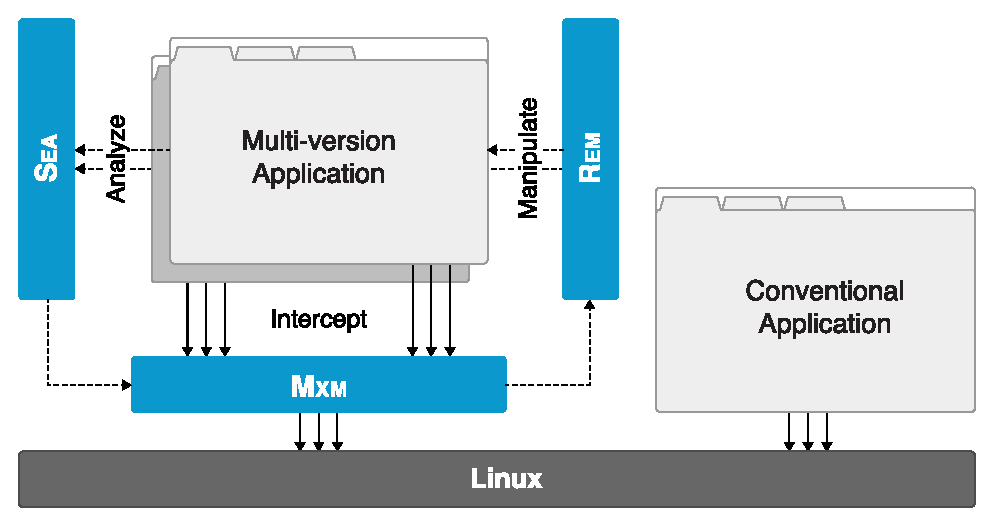
\includegraphics[width=\columnwidth]{safe-updates/figures/architecture}
\caption{\mx system architecture.  
%% The main components of \mx
%%   are \sea (Static Executable Analyser), \mxm (Multi-eXecution
%%   Monitor), and \rem (Runtime Execution Manipulator).
}
\label{fig:design}
\end{center}
\end{figure}


\subsection{System call interposition}
\label{sec:mxm}

One of the main components of our multi-version execution environment
is the \mxm monitor.  \mxm's main jobs are to run the two versions
concurrently, mediate their interaction with the outside world,
synchronise their executions, and detect any divergences in their
external behaviour. \mxm works by intercepting all system calls issued
by each application version, and manipulating them to ensure that the
two versions are executed in a synchronised fashion and act as one to
the outside world.

\mxm provides functionality similar to conventional virtual machine
monitors.  Whenever the MV application is executed, the \mxm connects
to all application versions running in parallel, intercepting their
kernel system calls.  \mxm ensures that the two versions act as one to
the outside world by mediating access to the underlying operating
system to achieve complete isolation of the running application from
other application instances as well as from the external environment,
making sure the combined application versions act as one to the
outside world.  The environment controlled by the monitor consists
mainly of a restricted file system access, socket interceptors and
signal handlers.

\subsubsection{System call interception}

\mxm is implemented using the  \ptrace interface provided by the Linux
kernel.  This interface, often used for application debugging, allows
simple deployment (without any need for compile-time instrumentation)
and makes the monitor itself lightweight since it is running as a
regular unprivileged process.  \mxm is similar in operation to previous
monitors whose goal is to synchronise applications at the level of system
calls such as Orchestra~\cite{orchestra09}, PLR~\cite{shye2009} or
Tachyon~\cite{tachyon12}.

\mxm runs each version in a separate child process, intercepting all
their system calls.  When a system call is intercepted in one version,
\mxm waits until the other version also performs a system call.  With
a pair of system calls in hand (one executed by the old version, and
one by the new version), \mxm compares their types and arguments.  If
they differ, \mxm has detected a divergence and invokes the \rem
component to resolve it (\S\ref{sec:rem}).

Otherwise, if the two versions perform the same system call with the
same arguments, \mxm virtualises their interaction with the
environment.  If the operation performed by the system call has no
side effects and does not involve virtualised state (\eg
\textstt{sysinfo}), \mxm allows both processes to execute it
independently.  Otherwise, it executes the system call on their
behalf and copies its results into the address spaces of both
versions.

\mxm must also enforce deterministic execution across versions. This
consists mainly of intercepting instructions that may produce
non-deterministic results, and returning the same result in both
versions.  Examples of such non-deterministic operations include
random number generators (\eg read calls to \textstt{/dev/[u]random}),
date and time (\eg read calls to \textstt{/etc/localtime}), and access
to files and network (\eg file descriptor consistency).  Note that
non-deterministic effects resulting from allocating memory objects at
different addresses in memory or randomly arranging memory areas via
address space layout randomisation (ASLR) do not pose any
problems: \mxm understand the semantics of individual system calls and
rather than directly comparing memory addresses (which might be
different in each executed version), it compares the actual values
stored at those memory locations. \mxm support both memory buffers (by
comparing the actual buffer content) as well as data structures
referenced by pointers (including nested ones).
 
Since \mxm fully controls executing programs intercepting all their
system calls, it can ensure that both programs have the same view of
their environment.

Whenever the monitored process makes a system call, \mxm is notified
twice---first before, then after the call has been executed.  When a
\ptrace event is raised (\eg a new child process has been started),
the monitor is notified as well.  Due to internal limitations of the
\ptrace interface, once the system call has been made, it cannot be
skipped, so when \mxm wants to execute the call on behalf of its child
processes, it simply replaces it with a system call that does not
change the system state (\texttt{getpid} in our case).

There are several challenges that we encountered while implementing
\mxm.  First, \mxm must partly understand the semantics of 
system calls.  For example, many system call parameters use complex
(often nested) structures with complicated semantics to pass values to
the operating system kernel, as in the case of \textstt{ioctl} or
\textstt{futex}.  To be able to compare the parameters of
these system calls and copy back their results, \mxm needs to
understand the semantics of these structures.  However, there are only
a relatively small number of system calls in Linux, and once the support
for handling them is implemented, it can be reused across applications.
\mxm currently implements \syscallsImplemented system calls (out of the
\syscallsTotal provided by Linux x86-64 3.1.9), which was enough to
allow us to run \mx on our benchmarks
(\S\ref{sec:evaluation}).

Second, the arguments of a system call are often passed through pointers,
which are only valid in the application address space, which is not directly
available to \mxm.  Therefore, \mxm needs to copy the contents pointed to by
these structures to its own address space in order to perform their
comparison.  The \ptrace interface on x86-64 only allows to copy one quadword
per system call, which is very expensive. Previous approaches either used
various ad-hoc optimisations~\cite{orchestra09} such as named pipes or shared
memory with custom shellcode, or a modified kernel~\cite{tachyon12} to
overcome this limitation. Instead, \mxm uses \emph{cross memory attach}, a new
mechanism for fast interprocess communication which has been recently added to
the Linux kernel~\cite{crossmemoryattach}.  This mechanism provides two new
system calls---\textstt{process\_vm\_readv} and
\textstt{process\_vm\_writev}---which allows tracer to directly access the
memory space of tracee using an interface similar to \textstt{readv} and
\textstt{writev} system calls without any additional overhead.

Third, because the structures passed as arguments to system calls often have
variable-size, \mxm also needs a fast way to allocate and deallocate memory
for them in order to minimise the overall overhead imposed by our system.  For
this purpose, \mxm uses a region-based memory allocator~\cite{memory-pools},
namely the \textstt{obstack}
library\footnote{\url{http://www.gnu.org/software/hello/manual/libc/Obstacks.html}}.
which is part of the GNU C Library.  Each monitored process has its own
obstack, which is used for allocating memory to store the copy of the process'
system call arguments

\subsubsection{Multi-process and multi-threaded applications}

Finally, a particular challenge arises in the context of multi-process and
multithreaded applications.  Using a single monitor instance to intercept both
versions and their child processes (or threads) would eliminate any advantage
that these applications derive from using concurrency.  Therefore, \mxm uses a
new monitor thread for each set of child processes (or threads) spawned by the
application.  For instance, if the old and new versions each have a parent and
a child process, then \mxm will use two threads: one to monitor the parent
processes, and one to monitor the child processes in each version.

Due to limitations of the \ptrace interface (which was not designed to be used
in a multi-process/multithreaded environment), handing the control of any
child processes being spawned by the application over to a new monitoring
thread is somewhat complicated.  In \mxm we adopt the solution similar to
Orchestra~\cite{orchestra09}.  When a new child process is spawned, we let the
parent monitoring thread to supervise its execution until the first system
call.  Then, we replace this system call with a \textstt{pause} system call,
disconnect the parent monitor (which causes a \textstt{continue} signal to be
sent to all new child processes), and spawn a new monitoring thread which
immediately reconnects to the new child process, restores its original system
call, and resumes its execution.

\mxm does not enforce deterministic execution across multiple versions of
multithreaded programs (which may diverge if race conditions can lead
to different external behaviour across executions), although we could
overcome this limitation by combining it with recently proposed
deterministic multithreading systems such
as \textsc{Dthreads}~\cite{dthreads:sosp11}.

%% \mxm also performs a series of optimisations to decrease performance
%% overhead, such as allowing certain files with read-only permissions
%% to be opened directly by the process. 

\subsubsection{Environment virtualisation}

To improve I/O performance and decrease virtualisation overhead,
processes are allowed to open files with read-only permissions
directly, while files with write permissions are opened by the monitor
itself.  This imposes another problem as file descriptors assigned to
these files are not necessarily the same in each version (\eg due to
scheduling non-determinism). Therefore, the \mxm needs to virtualise
these file descriptors.

Whenever monitored process opens a file with read-only permissions, a
new virtual file descriptor is assigned to this file together with the
mapping to a real file descriptor for each version. This virtual file
descriptor is then send to each version. When system call is made
using this virtual file descriptor, the \mxm replaces it with real
file descriptor before executing the system call. The actual file
operation is then executed by the process itself avoiding any memory
copying by the \mxm.

The similar approach is also used for virtualisation of process,
group, parent and child identifiers.  Whenever process tries to obtain
the actual ID, the \mxm replaces this with a virtual ID and keeps the
mapping between the real and the virtual ID. When process invokes a
system call using this ID as an argument (\eg \texttt{kill}), the
virtual ID is replaced with actual ID before executing the system
call.

%% \paragraph{Para-virtualisation interface and binary translation.}
%% Furthermore, we plan to combine this API with a binary translation
%% approach~\cite{binary-translation}, that will allow to dynamically
%% replace certain system calls with more efficient \emph{monitor
%% call} instructions.  The binary translation could be also used to
%% dynamically replace code components that have been proved to be
%% safe and do not need to be replicated across multiple versions (\eg
%% using static verification during compilation, using traces of
%% previous execution, using runtime heuristics).


%% \paragraph{Future work}

%% The \texttt{ptrace} interface allows us to easily monitor the program
%% execution without any compile-time instrumentation.  The main downside
%% of this approach is a relatively high overhead.  This is especially
%% true for I/O intensive applications, as they require frequent
%% transfers of large portions of the application memory space to the
%% monitor process. This overhead could be eliminated by directly
%% accessing the process memory space.

%% The existing prototype implementation of \textsc{Mxm} already supports
%% simple scenarios. The main limitation of this implementation is the
%% strict ordering of system calls, which must be the same in each
%% monitored application version.  To be practically usable, future
%% versions of \textsc{Mxm} need to relax the requirement on strict
%% ordering to allow more complex scenarios. This is especially important
%% when executing different versions of the same application.

%% Most importantly, a straightforward comparison of system call traces
%% is usually not sufficient to identify divergences, since different
%% versions might use a slightly different sequence of kernel and library
%% calls to implement the same behaviour.  We plan to explore approaches
%% similar to those implemented by compiler optimisations, such as
%% \emph{peep-hole optimisation}~\cite{dragon-book}, and adapt them to
%% work on the level of kernel and library calls.


%% %% \paragraph{Hashing system call traces.}
%% %% To decrease the overhead of kernel and library call synchronisation, we aim to
%% %% enhance our system to hash the sequence of system call traces using fast hash
%% %% functions such as FNV-1 or FNV-1a.  This approach has a significant advantage
%% %% over straightforward comparison of call traces, especially in the case of
%% %% system calls with virtually unlimited parameter sizes such as \texttt{read} or
%% %% \texttt{write}~\cite{shye2009}.  Similar approach has been already used
%% %% in~\cite{shye2009}.

%% \paragraph{Libraries support and virtualisation.}
%% Since many applications today use functionality provided by shared
%% libraries, we aim to support intercepting calls to such libraries as
%% well. Moreover, as intercepted calls to shared libraries can be
%% executed only once, same as in the case of system call monitoring,
%% this may decrease the overall overhead of multi-version execution.

%% We also plan to provide our own implementation of the \texttt{libc}
%% library loaded using the \texttt{LD\_PRELOAD} mechanism.  This library
%% will communicate directly with the monitor process through shared
%% memory, decreasing the number of system calls that need to be directly
%% intercepted, and thus resulting in much better performance.  However,
%% since the \texttt{LD\_PRELOAD} mechanism can be overridden, we still
%% need to combine it with the \texttt{ptrace} monitoring facility to
%% achieve complete isolation with reasonable overhead.  This approach
%% can be extended to support other shared libraries as well, further
%% improving the overall performance of our approach.

\subsection{Runtime state manipulation}
\label{sec:rem}

At the core of our system lies the \rem component, which is invoked
by \mxm whenever a divergence is detected.  \rem has two main jobs:
(1)~to decide whether to resolve the divergence in favour of the old or
the new version; and (2)~to allow the other version to execute through
the divergence and resynchronise the execution of the two versions
after the divergence.
%% The first task by itself it's easy: we favour the new version, except
%% for when it crashes.
%% As discussed in \sref{sec:scope}, in this paper we restrict our
%% attention to surviving crash errors, so the first task is relatively
%% easy: if one of the two versions crashes, we use the output of the
%% other version; otherwise, we always favour the new version.  
%%
%% The second task is however more difficult, but essential to the
%% success of our approach, which relies on having both versions be alive
%% at all times, so that the overall application can survive any crash
%% bugs that happen in either the old or the new version (although of
%% course, not in both).
%%
As discussed before, in \mx we focus our attention on surviving
crash errors, so the key challenge is to allow the crashing version to
survive the crash.  This is essential to the success of our approach,
which relies on having both versions alive at all times, so that
the overall application can survive any crash bugs that happen in
either the old or the new version (although of course, not in both at
the same time).

We emphasise that we apply our approach only to crash errors (those
raising a \textstt{SIGSEGV} signal), and not to other types of program
termination, such as \textstt{abort}s.  This is important from a
security perspective, because
%% many patches turn potential compromises into
%% run-time {\small{\texttt{abort}s}}, \eg using assertions for input
%% sanitisation.  For example, 
when a vulnerability is discovered, but a proper solution is not yet
known, developers often
\footnote{For example, see the patch in json-cpp \url{http://jsoncpp.svn.sourceforge.net/viewvc/jsoncpp/trunk/jsoncpp/include/json/assertions.h?r1=247&r2=246&pathrev=247}}
fail-stop the program rather than letting it continue and allowing
the attacker to compromise the system.\looseness=-1
%
%% Such situations can be easily distinguished since failed assertions
%% result in program abortion (\ie
%% \textstt{SIGABRT} signal), while unintentional program crashes typically
%% result in abnormal termination (\ie \textstt{SIGSEGV} signal). 
%% Therefore, \rem only intercepts and handles crashes resulting
%%   in \textstt{SIGSEGV} signals.

Suppose that one of the versions has crashed between the execution of
system call $s_1$ and the execution of system call $s_2$.  Then, in
many common scenarios, the code executed between the two system calls
is responsible for the crash (\eg the old version crashes because it
doesn't incorporate a bug fix present in the new version, or the new
version crashes because its code was patched incorrectly).  Therefore,
our strategy is to do a form of \textit{runtime code patching}, in
which we use the code of the non-crashing version to execute over the
buggy code in the crashing version.

%% If the behaviour of the two versions is different, but they both
%% continue to execute, then we favour the behaviour of the new version and
%% wait for the two versions to reconverge.

%% There are many different ways to achieve this goal, such as the use of
%% a mechanism based on check-pointing and roll-back~\cite{qin2005};
%% however, these mechanisms cannot deal with persistent errors which are
%% common in the case of software updates.

%% Our solution is based upon the observation that errors in programs are
%% usually located at particular places (\ie specific instructions) in
%% the program's code.  Therefore, we can use the code of the other, and
%% \ie correct, version to execute over this critical point in program's
%% code. This approach may not work when memory layout of the two
%% versions differs, as the code of one version may fail to locate the
%% memory structures necessary for its execution in the memory of the
%% other version. Nevertheless, the described approach might still work
%% in many cases when memory layout of the two versions does not differ
%% significantly.


%\paragraph{Possible execution scenarios.}

%% We run two versions of the same application in parallel, monitoring
%% their execution to be sure that they behave in the same way without
%% any divergences by comparing the application executions at
%% synchronisation points; in case of our prototype equal to system
%% calls. When either of the versions fail, we stop its execution at the
%% \emph{divergence point}; at this point there are three possible
%% solutions to synchronise the divergent versions:

\begin{figure}[t]
\centering
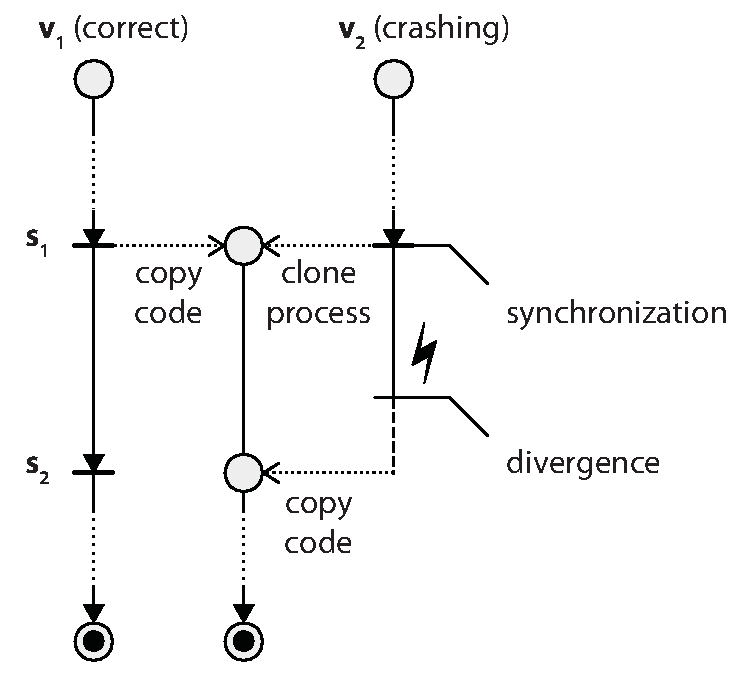
\includegraphics[width=0.8\columnwidth]{safe-updates/figures/strategy}
\caption{\rem's recovery mechanism uses the code of the non-crashing
  version to run through the buggy code.}
\label{fig:solution3}
\end{figure}

%% \begin{enumerate}[label=\emph{S\arabic*}, itemsep=3pt, parsep=3pt]
%% \renewcommand*\labelitemi{\emph{S\arabic*}}
%% \begin{figure}[t]
%%   \centering
%%   \subfloat[Patch state after the crash and continue execution]{
%%     \includegraphics[width=0.45\columnwidth]{safe-updates/figures/solution1}
%%     \label{fig:solution1}
%%   }
%%   \quad
%%   \subfloat[Patch state before the crash and continue execution]{
%%     \includegraphics[width=0.45\columnwidth]{safe-updates/figures/solution2}
%%     \label{fig:solution2}
%%   }
%%   \\
%%   \subfloat[Use the code of older version only to run through critical section]{
%%     \includegraphics[width=0.45\columnwidth]{safe-updates/figures/solution3}
%%     \label{fig:solution3}
%%   }
%%   \caption{Three solutions for synchronising two divergent versions of
%%   the same application}
%%   \label{fig:solution}
%% \end{figure}

%% \item\label{s1} Clone the correctly executing version to duplicate its state
%%   (\eg memory content, memory mappings) after the crash and replace its
%%   code with the code of the failed version. Then restart both versions and
%%   continue their execution (Figure~\ref{fig:solution1}).

%% \item\label{s2} Clone the correctly executing version to duplicate its state
%%   (\eg memory content, memory mappings) at the last synchronisation point (\ie
%%   creating checkpoint). After the crash, replace the code of this cloned
%%   version with the code of the failed version. Then restart this cloned
%%   version, execute over the \emph{critical section}, and continue execution of
%%   both versions (Figure~\ref{fig:solution2}).

%% \item\label{s3} Clone the failing version to duplicate its state (\eg memory
%%   content, memory mappings) at the last synchronisation point (\ie creating
%%   checkpoint). After the crash, replace the code of this cloned version with
%%   the code of the correctly executing version. Then restart this cloned
%%   version; after the application successfully executes over the \emph{critical
%%   section}, replace the code of the cloned version again with the original
%%   code, and continue its execution (Figure~\ref{fig:solution3}).

%% \end{enumerate}

Our exact recovery mechanism is illustrated in
Figure~\ref{fig:solution3}.  At each system call, \mx creates a
lightweight checkpoint of each version.  This is implemented using the
\textstt{clone} system call in Linux, which internally uses a
copy-on-write strategy.  
%% As an important optimisation, we omit system
%% calls that can be replayed safely from the last checkpoint, such
%% as \textstt{read}.

As shown in Figure~\ref{fig:solution3}, suppose that the crash happens
in version $v_2$, between system calls $s_1$ and $s_2$.  Then, \rem
first restores $v_2$ at point $s_1$, copies $v_1$'s code into $v_2$'s
code segment, executes over the buggy code using $v_1$'s code (but
note that we are still using $v_2$'s memory state), and then restore
$v_2$'s code at point $s_2$.

There are several challenges in implementing this functionality.
First, \rem needs the ability to read and write the application code
segment.  In the current implementation, we bypass this by linking
together the two application versions after renaming all the symbols
in one of the versions using a modified version of
the \textstt{objcopy}
tool.\footnote{\url{http://sourceware.org/binutils/docs/binutils/objcopy.html}}
However, in the future we plan to implement this transparently by
using the cross-memory attach mechanism used by \mxm.
%% \textstt{pread} and \textstt{pwrite} interface to directly
%% read and write the process memory via the
%% %\textstt{/proc/<pid>/mem} file in the
%% \emph{proc} file system.

%% This functionality has been recently introduced to the Linux kernel in
%% version 2.6.39~\cite{kernel-procmem}; previously, this interface was
%% read-only. This approach imposes only minimal overhead as it allows
%% direct access to the process memory space.

%% The runtime process manipulation functionality is implemented inside
%% \rem, a separate component used by the \mxm monitor. The
%% manipulation itself is driven by the data obtained statically by the
%% \sea analyser before the application has been executed.

Second, \rem needs to modify the contents of the stack in $v_2$.  This
is necessary because the return addresses on the stack frames of $v_2$
still point to $v_2$'s original code, which was now replaced by
$v_1$'s code.  Without also modifying $v_2$'s stack, any
function \textstt{return} instruction executed between $s_1$ and $s_2$
would most likely veer execution to an incorrect location, since
function addresses are likely to be different across different
versions.  Thus, after \rem replaces $v_2$'s code, it also updates the
return addresses on $v_2$'s stack with the corresponding return
addresses in $v_1$, which are obtained via static analysis
(\S\ref{sec:sea}).  Because system calls are invoked via wrapper
functions in \textstt{libc}, this ensures that when $v_2$ resumes
execution, it will immediately return to the code in $v_1$.
%% \rem obtains these addresses by analysing $v_1$'s stack at
%% position $s_1$ accessible via checkpoint taken at that point.
%
To implement this functionality, \rem makes use of
the \textstt{libunwind}
library,\footnote{\url{http://www.nongnu.org/libunwind/}} which provides a
portable interface for accessing the program stack, for both x86 and
x86-64 architectures. To actually modify the execution stack of
$v_2$, \rem uses again the \ptrace interface.


Unfortunately, updating the stack return addresses is not sufficient
to ensure that $v_2$ uses $v_1$'s code between $s_1$ and $s_2$, as
$v_2$ may also use function pointers to make function calls.
%% Note that we are still using the $v_2$ memory state. Thereby, $v_2$
%% may still issue a function call to the original code through one of
%% the function pointers.
To handle such cases, \rem inserts breakpoints to the first
instruction of every function in $v_2$'s original code.  Then, when a
breakpoint is encountered, \rem is notified via a \textstt{SIGTRAP}
signal, and redirects execution to the equivalent function in $v_1$'s
code (which is obtained from the \sea component) by simply changing
the instruction pointer.
%The address of the equivalent function is obtained

Finally, after executing through the buggy code, \rem performs the
same operations in reverse: it redirects execution to $v_2$'s original
code, changes the return addresses on the stack to point to $v_2$'s
functions, and disables all breakpoints inserted in $v_2$'s code.  
The one additional operation that is done at this point is to copy all
the global data modified by $v_1$'s code into the corresponding
locations referenced by $v_2$'s code.  

%\paragraph{Runtime stack analysis and manipulation.}

%% For example, on the x86 architecture, the stack can be easily
%% traversed starting from the top as each stack frame contains frame
%% pointer pointing to the previous stack frame, thereby forming a linked
%% list-like structure. This is not possible on the x86-64 architecture
%% as the frame pointer is no longer stored inside the stack frame.  To
%% traverse the execution stack on this architecture, it is necessary to
%% compute sizes of all functions' stack frames using the stack usage
%% information stored in the \texttt{UNWIND\_CODE} section, which is a
%% part of the ELF binary file. This logic is implemented by the
%% \texttt{libunwind} library, which provides API to unwind the stack
%% independent of the target platform.

%The necessary information about the stack location (\ie address range) and
%page mapping are obtained through the \emph{proc} file system; in particular
%the \textstt{/proc/<pid>/maps} and \textstt{/proc/<pid>/pagemap} files.

Note that \mx cannot currently handle major modifications to the
layout of the data structures used by the code, including individual
stack frames.  While this still allows us to support several common
software update scenarios, in future work we plan to improve the
system with the ability to perform full stack
reconstruction~\cite{upstare} and automatically infer basic data
structure changes at the binary-level~\cite{data-struct-digging}.
%% to identify changes to function names and sequences of function calls
%% (e.g., via clone detection techniques~\cite{cp-miner06,deckard07}),


Our approach of using the code of the non-crashing version to survive
failures in the crashing one may potentially leave the recovered
version in an inconsistent state. However, \mx is able to discover
most internal state inconsistencies by comparing whether the two
versions have the same external behaviour. When the behaviour of the
recovered version starts to differ, \mx will immediately discard it
and continue with only one version to ensure correctness. The
discarded version can be later restarted at a convenient
synchronisation point.  This restarting functionality is not currently
implemented in \mx, but we plan to add it as a future extension.

%Our approach of using the code of the non-crashing version to survive
%failures in the crashing one may leave the application in an
%inconsistent state, and thus may not be applicable for application in
%which absolute correctness and a fail-fast approach are more important
%than allowing the application to survive errors.  However, \mx is
%usually able to discover most internal state inconsistencies, since it
%regularly checks if the two versions have the same external
%behaviour. (See \S\ref{sec:discussion} for an extended discussion.)

\subsection{Binary static analysis}
\label{sec:sea}

%% \begin{table*}[t]
%% \centering 
%% \begin{tabular}{ccc}
%%   \hline
%%   Library calls in $\mathrm{version}_1$ & Library calls in $\mathrm{version}_2$ &
%%   System calls within the library \\
%%   \hline
%%   \texttt{<0xdeadbe5a>} & \texttt{<0xdeadbe8e>} &
%%   [\texttt{<0x77ff2c>}, \texttt{<0x77ffae>}] \\
%%   \texttt{<0xdeadabf5>} & \texttt{<0xdeadac34>} &
%%   [\texttt{<0x782bae>}] \\
%%   \vdots & \vdots & \vdots \\
%% \end{tabular}
%% \caption{Addresses of library function calls, and system calls invoked from
%% within these functions.}
%% \label{tab:syscall_table}
%% \end{table*}

The \sea component statically analyses the binaries of the two
versions to obtain information needed at runtime by the \mxm and \rem
components.  \sea is invoked only once, when the multi-version
application is assembled from its component versions.
%% As mentioned in \sref{sec:rem}, we currently link together the
%% two application versions after renaming all the symbols in one of them
%% using a modified copy of the \textstt{objcopy} tool, although in the
%% future we plan to do this linking dynamically by directly changing the
%% code segment in each version.

The main goal of \sea is to create several mappings from the code of
one version to the code of the other.  First, \sea extracts the
addresses of all function symbols
in one version and maps them to the
addresses of the corresponding functions in the other version.  This
mapping is used by \rem to handle calls performed via function
pointers (\S\ref{sec:rem}).

Second, \sea computes a mapping from all possible return addresses in
one version to the corresponding return addresses in the other version.  In
order to allow for code changes, this mapping is done by computing an
ordered list of all possible return addresses in each function.  For
example, if function \textstt{foo} in $v_1$ performs call instructions
at addresses \textstt{0xabcd0000} and \textstt{0xabcd0100}, and
function \textstt{foo} in $v_2$ performs call instructions at
addresses \textstt{0xdcba0000} and \textstt{0xdcba0400}, then \sea
will compute the mapping \textstt{\{0xabcd0005 $\rightarrow$
0xdcba0005, 0xabcd0105 $\rightarrow$ 0xdcba0405\}} (assuming each call
instruction takes 5 bytes).  This mapping is then used by \rem to
rewrite return addresses on the stack.

%% These data are gathered by the \sea analyser component which
%% implements static analysis of binary executables to extract all
%% necessary addresses and provide them to other components inside our
%% system. The format used for storing these data is represented by a
%% \emph{call table}. For each version, this table contains addresses of
%% all calls to shared library functions together with the list of all
%% system calls addresses invoked within these library functions, as can
%% be seen in Table~\ref{tab:syscall_table}.

%% For example, the first line of this table represents a call to a
%% library function which does two system calls, while second line
%% represents a function call which does only one system call.

To construct these tables, \sea first needs to extract the addresses
of all function symbols and then disassemble the code for each
individual function in order to locate the call instructions within
them.  The implementation is based on the \textstt{libbfd}
and \textstt{libopcodes} libraries, which are 
part of the
\gnu \binutils suite.\footnote{\url{http://www.gnu.org/software/binutils/}}
To obtain the addresses of all function symbols defined by the
program, \sea uses \textstt{libbfd} to extract the static and dynamic
symbol tables and relocation tables.  To disassemble individual
functions, \sea uses the \textstt{libbf}
library,\footnote{\url{http://github.com/petrh/libbf}} 
built on top of \textstt{libopcodes}.

%% Disassembled machine code is stored in a graph-like structure where
%% individual instructions represents vertices and edges between these
%% vertices represents the control flow. 

%% \paragraph{System call identification.}
%% \sea implementation uses the disassembler to obtain machine
%% code of each individual function and iterates over its instructions
%% (traversing the instruction graph) to identify basic blocks and locate
%% system call instructions within the code these functions.

%% To locate system calls within shared library function calls,
%% \sea first needs to obtain the set of exported library
%% functions and system calls within these functions using the above
%% described approach. Then, \sea analyses the application binary
%% itself and locates all function calls to the shared library using the
%% information extracted from relocation and procedure lookup tables
%% contained in ELF binaries.

%% Results of this analysis are stored in a hash table and tree structure
%% to allow quick access eliminating any unnecessary overhead when these
%% information are accessed during runtime. These data are then used to
%% construct the already described \emph{call table}, before the
%% application itself is executed.

%% \subsection{Limitations and Future Work}
%% \label{sec:limitations}
%% \input{limitations}

\section{Evaluation}
\label{sec:reliability-evaluation}

To evaluate our approach, we show that \mx can survive crash bugs in several
applications. %(\S\ref{sec:surviving}). We then examine the question of how
%far apart can be the versions run by \mx (\S\ref{sec:bounds}), and discuss
%\mx's performance overhead (\S\ref{sec:performance}).
We have evaluated \mx using a set of bugs in three applications: \gnu
\coreutils, \redis and \lighttpd. We discuss each application in turn below.

\subsubsection{\gnu \coreutils}
\label{sec:coreutils}

\begin{table}[t]
\begin{center}
\caption{Utilities from \gnu \coreutils, the crash bugs used, and the 
versions in which these bugs were introduced and fixed.  We group
together utilities affected by the same or similar bugs.}
\begin{tabular}{lll}
\toprule
\textsc{Utility} & \textsc{Bug description} & \textsc{Bug span} \\
\midrule
\mdsum & \multirow{2}{*}{Buffer underflow} & \multirow{2}{*}{v5.1 -- v6.11} \\
\shasum & & \\
\midrule
\mkdir & \multirow{2}{*}{\textstt{NULL}-pointer dereference} & \multirow{2}{*}{v5.1 -- v6.11} \\
\mkfifo & & \\
\mknod & & \\
\midrule
\cut & Buffer overflow & v5.3 -- v8.11 \\
\bottomrule
\end{tabular}
\label{tbl:cu-bugs}
\end{center}
\end{table}

The \gnu \coreutils utility
suite\footnote{\url{http://www.gnu.org/software/coreutils/}} provides
the core user-level environment on most UNIX systems.  We have selected
a number of bugs reported on the \coreutils mailing list, all of which
trigger segmentation faults.  The bugs are described in
Table~\ref{tbl:cu-bugs}, together with the utilities affected by each
bug and the versions in which they were introduced and fixed.

The bug affecting both \mdsum and \shasum utilities, introduced in version 5.1
and later fixed in version 6.11, caused a crash due to a buffer underflow when
checking an invalid BSD-style input. Another bug we have considered affected
\mkdir, \mkfifo and \mknod utilities; this bug, which was reported in 6.10 and
fixed in 6.11 resulted in a crash when accessing an invalid context.  Finally,
the bug affecting the \cut utility, introduced in 5.3 and later fixed in 8.11,
resulted in a segmentation fault when using a large unbounded range. 

For all these bugs, we configured \mx to run the version that fixed the
bug together with the one just before. We could have also run the
version that introduced the bug with the one just before, but we could
not immediately tell where the bug was introduced, and we cannot build
versions earlier than 6.10 due to changes in GCC and GNU C library. \mx
successfully intercepted the crash and recovered the execution by using
the strategy described in Section~\ref{sec:rem}.

We discuss below the bug in the \cut utility (used to remove sections
from each line of a file), triggered by the following invocation:

\begin{lstlisting}[numbers=none,breaklines=true,xleftmargin=0pt,language=bash]
cut -c1234567890- --output-d=: foo
\end{lstlisting}

This bug is triggered by the conditional statement on line~\ref{line:cond}:

\begin{lstlisting}[firstnumber=525]
if (output_delimiter_specified /*@\label{line:cond}@*/
    && !complement
    && eol_range_start && !is_printable_field (rsi_candidate))
\end{lstlisting}

This code uses the lower bound of the size of the printable field
vector; however, when calculating the size of this vector, ranges going
to the end of line (\ie \lstinline`0-`) are not considered, eventually
resulting in an invalid memory access. The cause of this bug is an incorrectly
calculated size of a dynamically allocated buffer, which is later used by the
program, leading to a buffer overflow. When \mx intercepts this bug, it uses
the last checkpoint to recover the execution of the crashing version. This
checkpoint is taken after the \lstinline`brk` system call triggered by the
\lstinline`malloc` call that allocates the buffer in function
\lstinline`bindtextdomain` on line~\ref{line:bind}.

\begin{lstlisting}[firstnumber=767]
bindtextdomain (PACKAGE, LOCALEDIR); /*@\label{line:bind}@*/
\end{lstlisting}

The recovered process uses the code of the other version to correctly
calculate the size of the field vector and switches back to the original
code during the allocation of this buffer, as
%code during the allocation of this buffer on line~\ref{line:alloc} as
function \lstinline`xzalloc` triggers a \lstinline`mmap64` system call just
before executing the conditional statement on line~\ref{line:cond},
which originally triggered the bug.

\subsubsection{\redis}
\label{sec:redis}

Below, we describe how \mx can survive the \redis bug presented in
Section~\ref{multi-version:scenarios}; this bug, introduced during a code
refactoring, causes \redis to crash when the \lstinline`HMGET` command is used
with the wrong type. We are running in parallel the revision \textstt{a71f072f}
(\textit{the old version}, just before the bug was introduced) with revision
\textstt{7fb16bac} (\textit{the new version}, which contains the bug).  \mx
first invokes \sea to perform a static analysis of the two binaries and
construct the mappings described in \sref{sec:sea}.  Then, \mx invokes the \mxm
monitor, which executes both versions as child processes and intercepts their
system calls.

When the new version crashes after issuing the problematic
\textstt{HMGET} command, \mxm intercepts the \textstt{SIGSEGV} signal
which is sent to the application by the operating system.  At
this point, \rem starts the recovery procedure.  First, \rem sends a
\textstt{SIGKILL} signal to the new version to terminate it.  It then
restores the last checkpoint of the new version, which was taken at the
point of the last invoked system call, which in this case is an
\textstt{epoll\_ctl} system call.  Then, \rem uses the information
provided by \sea to rewrite the stack of the new version, as detailed
in \sref{sec:rem}.  In particular, \rem replaces the return
addresses of all functions in the new version with the corresponding
addresses from the old version. The stack rewriting itself however is not
enough. The newer version can still use function pointers, which are
part of the replicated state, to invoke the original code. To prevent
this situation, \rem inserts breakpoints at the beginning of all the
functions in the code of the new version (to intercept indirect calls
via function pointers), and then finally restores the original processor
registers of the checkpointed process and restarts the execution of the
(modified) new version.

Since the checkpoint was performed right after the execution of the system
call \textstt{epoll\_ctl}, the first thing that the code does is to
return from the \textstt{libc} wrapper that performed this system
call.  This in turn will return to the corresponding code in the old
version that invoked the wrapper, since all return addresses on the
stack have been rewritten.  From then on, the code of the old version
is executed (but in the state of the new version), until the first
system call is intercepted.  In our example, the old and the new
versions perform the same system call (and with the same arguments),
so \rem concludes that the two processes have re-converged, and thus
restores back the code of the new version by performing the steps
above in reverse, plus the additional step of synchronising their
global state (see \S\ref{sec:rem}).  Finally, the control is handed
back to the \mxm monitor, which continues to monitor the execution of
the two versions.

\subsubsection{\lighttpd}
\label{sec:lighttpd}

To evaluate \mx on \lighttpd, we have used two different crash bugs, \#1601 and
\#2140.  The first bug is the one described in detail in Section
\ref{multi-version:scenarios}, related to the ETag and compression
functionalities.  As previously discussed, the crash is triggered by a very
small change, which decrements the upper bound of a \textstt{for} loop by one.
\mx successfully protects the application against this crash, and allows the
new version to survive it by using the code of the old version.

The other crash bug we reproduced affects the URL rewrite
functionality.\footnote{\url{http://redmine.lighttpd.net/projects/lighttpd/issues/2140}}
This is also caused by an incorrect bound in a \lstinline`for` loop.
More precisely, the loop: 

\begin{lstlisting}[numbers=none,breaklines=true,xleftmargin=0pt]
for (k=0; k < pattern_len; k++)
\end{lstlisting}

\noindent should have been:

\begin{lstlisting}[numbers=none,breaklines=true,xleftmargin=0pt]
for (k=0; k@+1@ < pattern_len; k++)
\end{lstlisting}

The bug seems to have been present since the very first version
added to the repository.  It was reported in December 2009, and
fixed one month later.  As a result, we are running \mx using the last
version containing the bug together with the one that fixed it.  While
this bug does not fit within the pattern targeted by \mx (where a
newer revision introduces the bug), from a technical perspective it is
equally challenging.  \mx is able to successfully run the two versions
in parallel, and help the old version survive the crash bug.

%The bug \#1601 affects the HTTP redirection functionality, in particular
%the \texttt{\%n} substitution with condition substring. This functionality has
%been introduced in revision \texttt{510}. However, there is an incorrect
%comparison in one of the conditions which causes segmentation fault when
%appending matched parts to buffer if there was no matching regular expression.
%The affected code can be seen in Listing~\ref{lst:510}.

%\begin{lstlisting}[label=lst:510, caption={Original correct version of the function}]
%cond_cache_t *cache = &con->cond_cache[dc->context_ndx];
%if (n > cache->patterncount) {
  %return 0;
%}
%\end{lstlisting}

%The fix to this bug consists of a single changed line as can be seen in
%Listing~\ref{lst:2138} and has been incorporated in revision \texttt{2138}, yet
%this bug remained undetected for nearly three years (August 8, 2005 --- March
%26, 2008) rendering \lighttpd webserver vulnerable to attack.

%\begin{lstlisting}[label=lst:2138, caption={Refactored failing version of the function}]
%cond_cache_t *cache = &con->cond_cache[dc->context_ndx];
%if (n >= cache->patterncount) {
  %return 0;
%}
%\end{lstlisting}

Both \lighttpd bugs \#1601 and \#2140 are very simple---their fix consist of a
single character---yet still they made the \lighttpd server vulnerable to a
potential attack. \mx can not only handle the crash, but also successfully
recover the failing version in both cases.

\subsection{Ability to run distant versions}
\label{sec:bounds}

\begin{table}
\begin{center}
\caption{The maximum distance in number of revisions, and the time span
  between the revisions that can be run by \mx for each bug.}
\begin{tabular}{lcc}
\toprule
\textsc{Application Bug} & \textsc{Max distance} & \textsc{Time span} \\
\midrule
\lighttpd \#2169   & \maxDistLighttpdOne & \timeSpanLighttpdOne \\
\lighttpd \#2140   & \maxDistLighttpdTwo & \timeSpanLighttpdTwo \\
\redis \#344       & \maxDistRedis & \timeSpanRedis \\
%md5sum          & \maxDistMdsum & \timeSpanMdsum \\ \hline
\bottomrule
\end{tabular}
\label{tbl:bug-bounds}
\end{center}
\end{table}

In the previous sections, we have shown how \mx can help software
survive crash bugs, by running two \textit{consecutive} versions of an
application, one which suffers from the bug, and one which does not.
%
One important question is how far apart can be the versions run
by \mx.  To answer this question, we determined for each of the bugs
discussed above the most distant revisions that can be run together to
survive the bug.  

For the \coreutils benchmarks, we are able to run versions which are
hundreds of revisions apart: \maxDistMdsum~revisions (corresponding to
\timeSpanMdsum of development time) for the \mdsum/\shasum bug; 
\maxDistMkdir~revisions (\timeSpanMkdir of development time) for the 
\mkdir/\mkfifo/\mknod bug; and \maxDistCut~revisions (\timeSpanCut 
of development time) for the \cut bug.

The most distant versions for the first \lighttpd bug are
approximately two months apart and have \maxDistLighttpdOne~revisions
in-between, while the most distant versions for the second
\lighttpd bug are also approximately two months apart but have only
\maxDistLighttpdTwo~revisions in-between.  Finally, the most distant
versions for the \redis bug are \maxDistRedis~revisions
and \timeSpanRedis apart.  

Of course, it is difficult to draw any general conclusions from only
this small number of data points.  Instead, we focus on understanding
the reasons why \mx could not run farther apart versions for the bugs
in \lighttpd and \redis (we ignore \coreutils, for which we can run
very distant versions).
%% For the \coreutils bugs, the lower bound is the earliest
%% version that we could build and run on our machine (v6.10).  The
%% upper-bound for 
%
For \lighttpd issue \#2169, the lower bound is defined by a revision
in which a pair of \lstinline`geteuid` and \lstinline`getegid` calls
are replaced with a single call to \lstinline`issetugid` to
allow \lighttpd to start for a non-root user with GID~\lstinline`0`. \mx 
currently does not support changes to the order of system calls, but
this limitation could be overcome by using the rewrite rules for system call
sequences supported  by \varan (\S\ref{sec:patternmatching}). This would
allow \mx to recognise that the pair \textstt{geteuid()} and
\textstt{getegid()} could be matched with the call to
\textstt{issetugid()} (\S\ref{sec:applications}).

The upper bound for \lighttpd issue \#2169 adds a \textstt{read} call to
\textstt{/dev/[u]random}, in order to provide a better entropy source for
generating HTTP cookies.  This additional \textstt{read} call changed the
sequence of system calls, which \mx cannot handle, but which again could be
handled by \varan's rewriting rules.

For \lighttpd issue \#2140, both the lower and the upper bounds are
caused by a change in a sequence of \textstt{read()} system calls.  We
believe this could be optimised by allowing \mx to recognise when two
sequences of read system calls are used to perform the same overall
read.

%% Lower bound: the fix consists of request parser changes which resulted
%% in different sequence of \textstt{read()} system calls. The different
%% sequence of \textstt{read()} calls also marked the upper bound in this
%% case, defined by revision \lighttpdTwoUB. In this revision, the way in
%% which input connection buffer is being filled has changed, fixing
%% issue \#2147 and CVE-2010-0295 vulnerability.

For the \redis bug, the lower bound is given by the revision in which the
\textstt{HMGET} command was first implemented.  Since there was no support for
\textstt{HMGET} before that version, \mx has no way to survive the crash caused
by invoking \textstt{HMGET} with a wrong type (see \S\ref{sec:redis}).  The
upper bound is defined by a revision which changes the way error responses are
being constructed and reported, which results in a very different sequence of
system calls.

%% , including the call on line
%% \ref{line:report-error2} in Listing~\ref{lst:refactored}, resulting in
%% different sequence of system calls.

%% \todo{explain that all of these changes are minor and some of them could be
%% very well handled by using window-based/peep-hole approach}

\subsection{Performance overhead}
\label{sec:performance}

\begin{figure}[!t]
\centering
\includegraphics[width=\textwidth]{safe-updates/graphs/spec2006}
\caption{Normalised execution times for the \speczerosix benchmark suite
running under \mx.}
\label{fig:spec}
\end{figure}

We ran our experiments on a four-core server with 3.50~GHz Intel
Xeon E3-1280 and 16~GB of RAM running 64-bit Linux v3.1.9.

\begin{enumerate}
\item[\speczerosix] To measure the performance overhead of our prototype, we
  first used the standard
  \speczerosix\footnote{\url{http://www.spec.org/cpu2006/}} benchmark suite.
  Figure~\ref{fig:spec} shows the performance of \mx running two instances of
  the same application in parallel, compared to a native system. The execution
  time overhead of \mx varies from \minOverSPEC to \maxOverSPEC compared to
  executing just a single version, with the geometric mean across all
  \numSPECbench benchmarks at \avgOverSPEC. This result is comparable with
  previous work using multi-variant execution that used \speccpu to measure
  performance~\cite{orchestra09} (even though that work used \speczerozero).

%% The overhead varies from \minRedisOver to \maxRedisOver depending
%% on the operation being performed. This is the worst case overhead
%% we have seen among all tested application and comes mainly from the
%% fact that \redis is an in-memory database optimised for maximum
%% bare-hardware performance and is very sensitive to any additional
%% software layers.  Even a state-of-the-art hypervisor can incur an
%% $n$-fold slowdown, so the relatively high measure overhead is
%% therefore unsurprising.

\item[\gnu~\coreutils] The six \coreutils applications discussed in
  \sref{sec:coreutils} are mostly used in an interactive fashion via the
  command-line interface (CLI). In this context, a high performance
  overhead is acceptable as long as it is not perceptible to the user; prior
  studies have shown that response times of less than 100ms typically feel
  instantaneous~\cite{card:human_proc}. In many common use cases (\eg creating
  a directory, or using \cut on a small text file), the overhead of \mx was
  imperceptible---\eg creating a directory takes around \avgMkdirNative
  natively and \avgMkdirMx with \mx. For the three utilities that process
  files, we calculated the maximum file size for which the response time with
  \mx stays under the 100ms threshold.  For \cut, the maximum file size is
  \cutCutoffSize (with an overhead of \cutCutoffOver), for \mdsum
  \mdsumCutoffSize (\mdsumCutoffOver overhead), and for \shasum
  \shasumCutoffSize (\shasumCutoffOver overhead).

\item[\lighttpd] We used the
  \httpload\footnote{\url{http://www.acme.com/software/http_load/}}
  multiprocessing test client that is also used by the \lighttpd developers.
  This benchmark measures the end-to-end time as perceived by users. As a
  result, we performed two sets of experiments: (1) with the client and server
  located on the same machine, which represents the worst case performance-wise
  for \mx; and (2) with the client and server located on different continents
  (one in England and the other in California), which represents the best case.
  The overhead for \lighttpd varies from \minLighttpdRemote to
  \maxLighttpdRemote in the remote scenario, and from \minLighttpdOver to
  \maxLighttpdOver in the local scenario.  Despite the relatively large
  overhead in the local experiments, the remote overhead is negligible because
  times are dominated by the network latency (which in our case is over
  \SI{150}{\milli\second}).

\item[\redis] To measure the performance overhead for \redis, we used the
  \redisbenchmark\footnote{\url{http://redis.io/topics/benchmarks}} utility,
  which is part of the standard \redis distribution and simulates
  \textstt{GET}/\textstt{SET} operations done by $N$ clients concurrently, with
  default workload. As in the case of \lighttpd, we performed two sets of
  experiments, one for the local scenario and one for the remote scenario. The
  overhead for \redis varies, depending on the operation being performed, from
  \minRedisRemote to \maxRedisRemote in the remote scenario, and from
  \minRedisOver to \maxRedisOver in the local scenario. 

\end{enumerate}

Given the results presented hereinbefore, we believe \mx is most suitable for
scenarios for which its execution overhead does not degrade the performance of
the end-to-end task, such as the remote \redis and \lighttpd scenarios
discussed above, or interactive tasks such as those performed using
command-line utilities, where users would not notice the overhead as long as
the response time stays within a certain range. On the other hand, it is
clearly not suitable for applications requiring high-throughput, which is what
motivated us design the high-performance mechanism of \varan.

%% \mx's performance overhead is strongly correlated with the frequency of
%% system calls that have to be intercepted.  Therefore, we could also
%% imagine \mx being automatically turned on and off during execution,
%% depending on the frequency of system calls experienced by the
%% application.

%% and only checkpoint at epoch boundaries.  To make this approach viable, we also
%% need to record system calls in each epoch, so that they can be
%% replayed during recovery. Second, 

%% instead of using \textstt{clone}
%% directly, we could implement the checkpointing functionality as a
%% loadable kernel module and only store the part of the state needed for
%% recovery as in~\cite{flashback}. Finally, we could explore the
%% possibility of not intercepting system calls in certain parts of the
%% code that were previously shown to be safe and do not need to be
%% replicated across multiple versions (\eg similarly
%% to~\cite{onlinevalidation}).

%The measured overhead is higher than
%for the SPEC~CPU2006 benchmarks (with a slowdown of up to \maxRedisOver
%for some operations in \redis) and we are currently investigating the
%reasons for this slowdown.

%First, we could to synchronise versions at a coarser
%granularity, by using a window/epoch approach~\cite{compl-schedules11},
%and by performing certain synchronisations at the level of shared
%library calls.  Second, we could explore the possibility of not
%intercepting system calls in certain parts of the code that were
%previously shown to be safe and do not need to be replicated across
%multiple versions.  Finally, we could decrease the checkpointing
%overhead, by performing them at a lower frequency, and record the
%external behaviour since the last checkpoint, so that it can be
%successfully replayed during recovery (\eg as in Rx~\cite{rx}).

%We also examined how the frequency of system calls affects the
%performance overhead of application executed on top \mx.
%Figure~\ref{fig:syscall} shows the average number of system calls during
%the execution of SPEC~CPU2006.  Rather surprising result is the fact
%that \textsf{452.libquantum}, even though having the largest run time
%overhead had the lowest average number of system calls.  On the hand,
%the performance overhead of \textsf{400.perlbench}, despite having the
%highest average number system, was bellow average. \todo{What is the
%conclusion here?}

% For example, as we discuss in related work, our
% monitor \mxm is very similar to the monitor used by
% Orchestra~\cite{orchestra09}, which by employing various optimisations
% manages to obtain an average overhead of only about 15\% when
% synchronising two program variants at the level of system calls.  In
% terms of checkpointing, the Rx system~\cite{rx} implements a similar
% approach based on the Linux copy-on-write mechanism, and which through
% various optimisations manages to achieve a performance penalty of less
% than 5\% when checkpointing every 200 milliseconds.

\section{Discussion}
\label{safe-updates:discussion}

This section discusses in more detail the scope of our approach, its limitation
and the different trade-offs involved.

%% This section discusses in more detail the scope of our approach
%% with regard to (1) the type of applications and code changes that
%% could benefit most from our approach, and (2) the trade-off between
%% availability/reliability/availability and strict
%% correctness/performance/energy consumption.

\paragraph{CPU utilisation and memory consumption} \mx incurs a performance
overhead, as discussed in \sref{sec:performance}. In our experience, \mx is
applicable to interactive applications such as command-line utilities and
interactive applications, where the performance degradation is not noticeable
to the user. \mx is not applicable to servers requiring high-throughput or to
patches that fix performance bugs, as the system runs no faster than the
slowest version.  Both of of these issues are addressed by
\varan.\marginnote{12}

Our approach of using idle CPU time to run additional versions also increases
energy consumption and therefore might not be applicable to energy-constrained
devices such as smartphones. However, it is interesting to note that idle CPUs
are not ``free'' either: even without considering the initial cost of
purchasing the, an energy-efficient server consumes half its full power when
doing virtually no work---and for other servers, this ratio is usually much
worse~\cite{barroso2007}.

Similarly, \mx also doubles the memory consumption, which in practice is less
of an issue but could still lead to a performance degradation due to increased
memory pressure for some applications.

\paragraph{Memory-based communication.} The current \mx prototype does not
support shared memory, which is often used for efficient communication between
processes, as its use would be invisible to our system call interposition
mechanism. One way we could handle this scenario is by serialising all accesses
to shared memory using using a repeatable deterministic task
scheduler~\cite{russinovich:pldi96}. This approach has been used by Paranoid
Android~\cite{paranoid-android} in the same context.

\paragraph{Deployment strategy} While our approach eases the decision of
applying a software update---as incorporating a new version would never
decrease the reliability\marginnote{10} of the multi-version application---the
number of versions that can be run in parallel is limited, being dictated by
the number of available resources (\eg the number of available CPU cores).  As
a result, we need a deployment strategy to decide what versions to use.  For
example, we could always run the last $N$ released versions (where $N$ is the
number of available resources), or we could always keep a one-year old version,
etc.  This thesis focuses on designing and implementing multi-version execution
techniques, but in future work we plan to explore deployment strategies in more
detail.

\section{Summary}
\label{safe-updates:summary}

Software updates are an important part of the software development and
maintenance process. Unfortunately, they also present a high failure risk, and
many users refuse to upgrade their software, relying instead on outdated
versions, which often leave them exposed to known software bugs and security
vulnerabilities.

In this chapter, we have presented \mx, a multi-version execution system for
improving the software update process. Whenever a new program update becomes
available, instead of upgrading the software to the newest version, we run the
new version in parallel with the old one, and carefully synchronise their
execution to create a more secure and reliable multi-version application.

\mx supports off-the-shelf Linux applications and our evaluation has shown that
it can be applied successfully to several real applications such as
\gnu~\coreutils, \lighttpd, and \redis.


\chapter{Efficient Multi-version Execution}

The key component of multi-version execution system is a runtime monitor that
enables the execution of multiple versions in parallel. Unfortunately, existing
monitors impose either a large performance overhead and/or rely on intrusive
kernel-level changes that increase the size of the trusted computing base.
Moreover, none of the existing solutions scales well with the number of
versions, since the runtime monitor acts as a performance bottleneck.

While synchronization can be performed at different levels, the most common
approach is to do it at the level of system calls, for several different
reasons:  first, many patches do not change the the sequence of system calls,
\ie the program's \textit{external behavior} (\S\ref{sec:behavior-evolution}).
%Second, system calls are the main way in which the application communicates
%with the outside environment, and therefore the ultimate target of attackers.
Second, as the main communication mechanism between applications and the
environment, system calls must be virtualized in order to enable the multiple
versions to act as one to the outside world.

%With the widespread availability of multi-core processors, running multiple
%diversified variants or several different versions of an application in
%parallel is becoming a viable approach for increasing software security and
%reliability.  The key component of such N-version execution (NVX) systems is a
%runtime monitor that enables the execution of multiple versions in parallel.

%In this chapter, we introduce \nx, a multi-version execition framework that
%combines binary rewriting with a novel event-streaming architecture to
%significantly reduce performance overhead and scale well with the number of
%versions, without relying on intrusive kernel modifications.

%Our evaluation shows that \nx can be used to run multi-version applications
%based on a number of popular C10k network servers with only a modest
%performance overhead.

The main challenge in implementing a multi-version execution monitor at the
system call level is the trade-off between performance, security, flexibility
and ease of debugging.  Many
implementations~\cite{orchestra09,tachyon12}, including
Mx (\S\ref{sec:mx}), use the \stt{ptrace} mechanism offered by most UNIX-based
operating systems.  While easy-to-use and not requiring kernel modifications,
\stt{ptrace} is slow, and these systems see performance degradations of up to
two orders of magnitude. A much faster approach is to implement the monitor in
kernel space~\cite{cox2006}, but this requires kernel patches and/or new kernel
modules, and more importantly leads to an increased trusted computing base, as
the monitor runs in privileged mode.  Furthermore, none of these approaches
scale well with the number of variants (as the monitor is both a communication
and synchronization bottleneck), none are debug-friendly (\stt{ptrace}
disallows the use of \stt{gdb}, while kernel debugging has its well-known set
of limitations) and none of them have been designed to be flexible with respect
to small variations in system call sequences (which can occur for certain
diversification transformations and across program versions).

%In this chapter, we introduce \nx, a multi-version execution framework that
%combines binary rewriting with a novel event-streaming architecture to
%significantly reduce performance overhead and scale well with the number of
%versions, without relying on intrusive kernel modifications.

In this chapter, we introduce \nx,\footnote{\varan's name comes from the
scientific name \emph{Varanus}, commonly known as the \emph{monitor} lizard.
Varan is also a name of the Kaiju monster that first appeared in the 1958 movie
\emph{Varan the Unbelievable}.} a multi-version execution system that
combines binary rewriting with a novel event-streaming architecture to
significantly reduce performance overhead and scale well with the number of
versions, without relying on intrusive kernel modifications. \nx monitor
operates at the system call level, runs in user space (and therefore in
unprivileged mode), introduces a small performance overhead for popular C10k
network servers and negligible for CPU-bound applications, scale well with the
number of versions, and provide a flexible mechanism for handling small
divergences in the system calls sequences issued across versions.

\section{Overview}
\label{sec:overview}

Two key aspects influence the performance and flexibility of an NVX
system: system call interception and version coordination.  We discuss
each in turn below.

\subsection{System call interception}
\label{sec:interception}

%% \begin{enumerate}[(i)]
%% \item wait for the interrupt signaling the entry to a system call;
%% \item examine the registers to determine whether the system
%% call is of interest;
%% \item for any arguments passed by reference, copy the content of
%% the memory for the process address space if necessary;
%% \item if the system call is to be skipped (or performed by the monitor
%% on behalf of the application), replace the original system call with a
%% "null" system call (\ie \lstinline`getpid`);
%% \item restart the execution of the application to execute the system call;
%% \item wait for the interrupt signaling the exit from a system call;
%% \item obtain the process registers to read the system call return value;
%% \item for any output arguments, copy the referenced data from
%% the process address space if needed; and
%% \item continue the execution of the application.
%% \end{enumerate}

The biggest downside of existing system call monitors based on the
\ptrace interface is the high performance
overhead~\cite{orchestra09,tachyon12}.  For each system call
performed by each version, execution must switch to the monitor
process, which has to perform several additional system calls in order
%to be notified about system call entry and exit, 
to copy buffers to and from the version being monitored, nullify the
system call, \etc as shown earlier in
Figure~\ref{fig:lockstep-execution}.

For CPU-intensive applications which perform few system calls, this
overhead will be amortised, translating into a modest overall
slowdown.  However, for heavily I/O-bound applications, the slowdown
can be up to two orders of magnitude, which is unacceptable for many
real-world deployments.
%
Consequently, in order to implement a system call monitor with
acceptable overhead even for heavily I/O-bound applications, we need
to eliminate context switching to the monitor and back during
interception and eliminate the need for additional system calls.  
This is accomplished through a combination of selective binary
rewriting and an interprocess communication mechanism based on a
fast shared memory ring buffer.

%\vspace{0.1in} \noindent \textbf{Selective binary rewriting.}  
Whenever code is loaded into memory, \varan scans each code page to
selectively rewrite all system calls with jump instructions to dedicated
handlers.  Section \ref{sec:rewriting} discusses in detail the main
steps and challenges associated with this binary rewriting approach.

To eliminate the need for additional system calls during interception,
\varan uses a shared ring buffer to communicate between versions.  This
ring buffer is heavily optimised for performance: it is stored in
memory, allows largely lock-free communication, and does not require
the dispatch of events to different queues.  These aspects are
discussed in detail in Section~\ref{sec:streaming}.



\subsection{Event-streaming architecture}
\label{sec:coordination}

In prior NVX systems, versions are typically run in lockstep, with a
centralised monitor coordinating and virtualising their execution.
Essentially, at each system call, the versions pass control to the
monitor, which waits until all versions reach the same system call.
Once this happens, the monitor executes the system call and
communicates the result to each individual version.  If two or more
versions try to break the lockstep by executing different system
calls, the monitor needs to either terminate the entire application or
continue executing a subset of the versions in lockstep.

This approach has two key disadvantages.  First, the centralised
monitor is a bottleneck, which can have a significant impact on
performance.  Note that in addition to the synchronisation overhead,
this centralised monitor makes the NVX application execute at the
speed of the slowest individual version.

Second, this approach is totally inflexible to any divergence in the
sequence of system calls executed across versions.  This is an issue
both when running automatically-diversified variants, where certain
transformations may affect the external behaviour, and when running
existing software revisions, where changes in the sequences of
system calls can occur between revisions. 

\begin{figure}[t]
  \begin{center}
    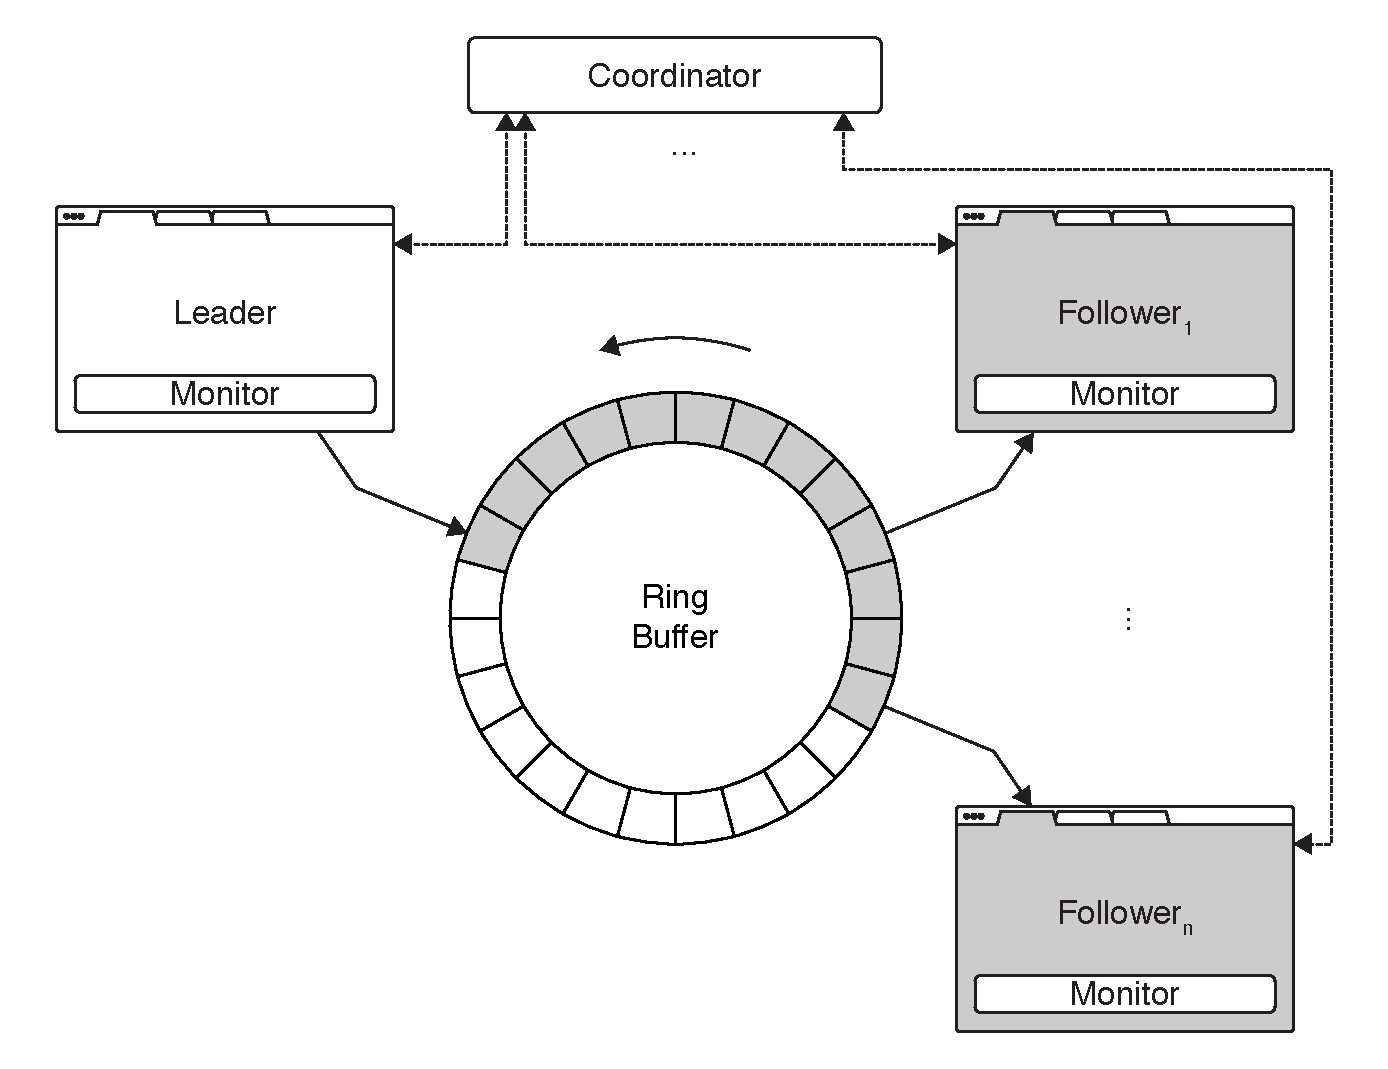
\includegraphics[width=0.6\textwidth]{efficient-execution/figures/architecture}
    \caption{The event-streaming architecture of \varan.}
    \label{fig:architecture}
  \end{center}
\end{figure}

To address these limitations, \varan uses a new approach which we call
\emph{event streaming}.  In this decentralised architecture,
depicted in Figure~\ref{fig:architecture}, one of the
versions is designated as the \textit{leader}, while the others are
\textit{followers}. During execution, the leader records all events into a
shared ring buffer, which are later read by followers to mimic the leader's
external behaviour (\S\ref{sec:streaming}). Events consist primarily
of regular system
call invocations, but also of signals, process forks (\ie \lstinline`clone`
and \lstinline`fork` system calls) and exits (\ie \lstinline`exit` and
\lstinline`exit_group` system calls).

In general, any version can be the leader, although in some situations
some may be a better choice than others, \eg when running multiple
software revisions in parallel, one might prefer to designate the
newest one as leader.  However, the leader can be easily replaced if
necessary, \eg if it crashes (\S\ref{sec:leader-repl}).

The only centralised component in this architecture is the
\textit{coordinator}, whose main job is to prepare the versions for
execution and establish the necessary communication channels.  At a
high level, the coordinator first loads the variants into memory,
injects several special handlers and memory objects into their address
spaces, rewrites any system calls in their code with jumps to the
special handlers and then starts executing the variants
(\S\ref{sec:setup}) in a decentralised manner.

%% recorded by one application version are shortly replayed
%% (\textit{streamed}) to the others, which keeps the log small, as
%% events which have been replayed by all versions can be discarded.
%% Similarly, the NVX context allows for the log to be kept in memory,
%% and for the replay to be done incrementally, with significant
%% performance advantages.  Event streaming is discussed in detail in
%% Section~\ref{sec:streaming}.


%% This is a variant of record-replay~\cite{scribe,jockey,geels06,r2},
%% but the NVX context allows us to overcome two of the main limitations
%% of traditional record-replay techniques, namely (1)~the
%% rapidly-growing log size, especially for system call-intensive
%% applications; and (2)~the long time necessary to replay the execution.
%% Because the multiple versions are executed concurrently, events
%% recorded by one application version are shortly replayed
%% (\textit{streamed}) to the others, which keeps the log small, as
%% events which have been replayed by all versions can be discarded.
%% Similarly, the NVX context allows for the log to be kept in memory,
%% and for the replay to be done incrementally, with significant
%% performance advantages.  Event streaming is discussed in detail in
%% Section~\ref{sec:streaming}.


\subsection{Rewrite rules for system call sequences}
\label{sec:rw}

In addition to eliminating the central monitor bottleneck, our
event-streaming architecture also supports (small) divergences between
the system call sequences of different variants.  For example,
different software revisions can be run inside a classical NVX
system only as long as they all issue the same sequence of system
calls~\cite{mx}.  However, software patches sometimes change the
external behavior of an application.  In particular, many divergences
in system call traces fall into the following two categories:
\begin{inparaenum}[(i)]
\item \emph{addition/removal}, characterising situations when one of
  the versions performs (or conversely does not perform) an additional
  system call, typically as a consequence of an additional check, and
\item \emph{coalescing}, covering the situations when a (repeated)
  sequence of system calls is executed a different number of times in
  each version (\eg one version might execute two \lstinline`write`
  system calls, while another version executes only one
  \lstinline`write` system call to write the same bytes because extra
  buffering is used).

\end{inparaenum}

% \begin{description}
%   \item[Addition/Removal] This class characterises situations when one
%     of the versions performs an additional system call (or conversely
%     does not perform), typically as a consequence of an additional
%     check.
%   \item[Coalescing] This class covers the situations when a (repeated)
%     sequence of system calls is executed a different number of times
%     in each version.  E.g., one version might execute two \lstinline`write`
%     system calls, while another a single equivalent \lstinline`write` to
%     write the same bytes (\eg because extra buffering is used).  
% \end{description}

\varan is the first NVX system that is able to deal with such changes.
When followers process the event sequence streamed by the leader, they
can rewrite it to account for any such differences: \eg they can skip
and merge system calls, or perform some calls themselves.  We provide
a flexible implementation of such rewrite rules using Berkeley Packet
Filters (\S\ref{sec:patternmatching}).


\section{\vx Prototype System}
\label{sec:prototype}

%% \begin{figure}[t]
%%   \begin{center}
%%     \includegraphics[width=\columnwidth]{figures/process-model}
%%     \caption{\vx process model.}
%%     \label{fig:process_model}
%%   \end{center}
%% \end{figure}

\begin{figure*}[t]
  \begin{center}
    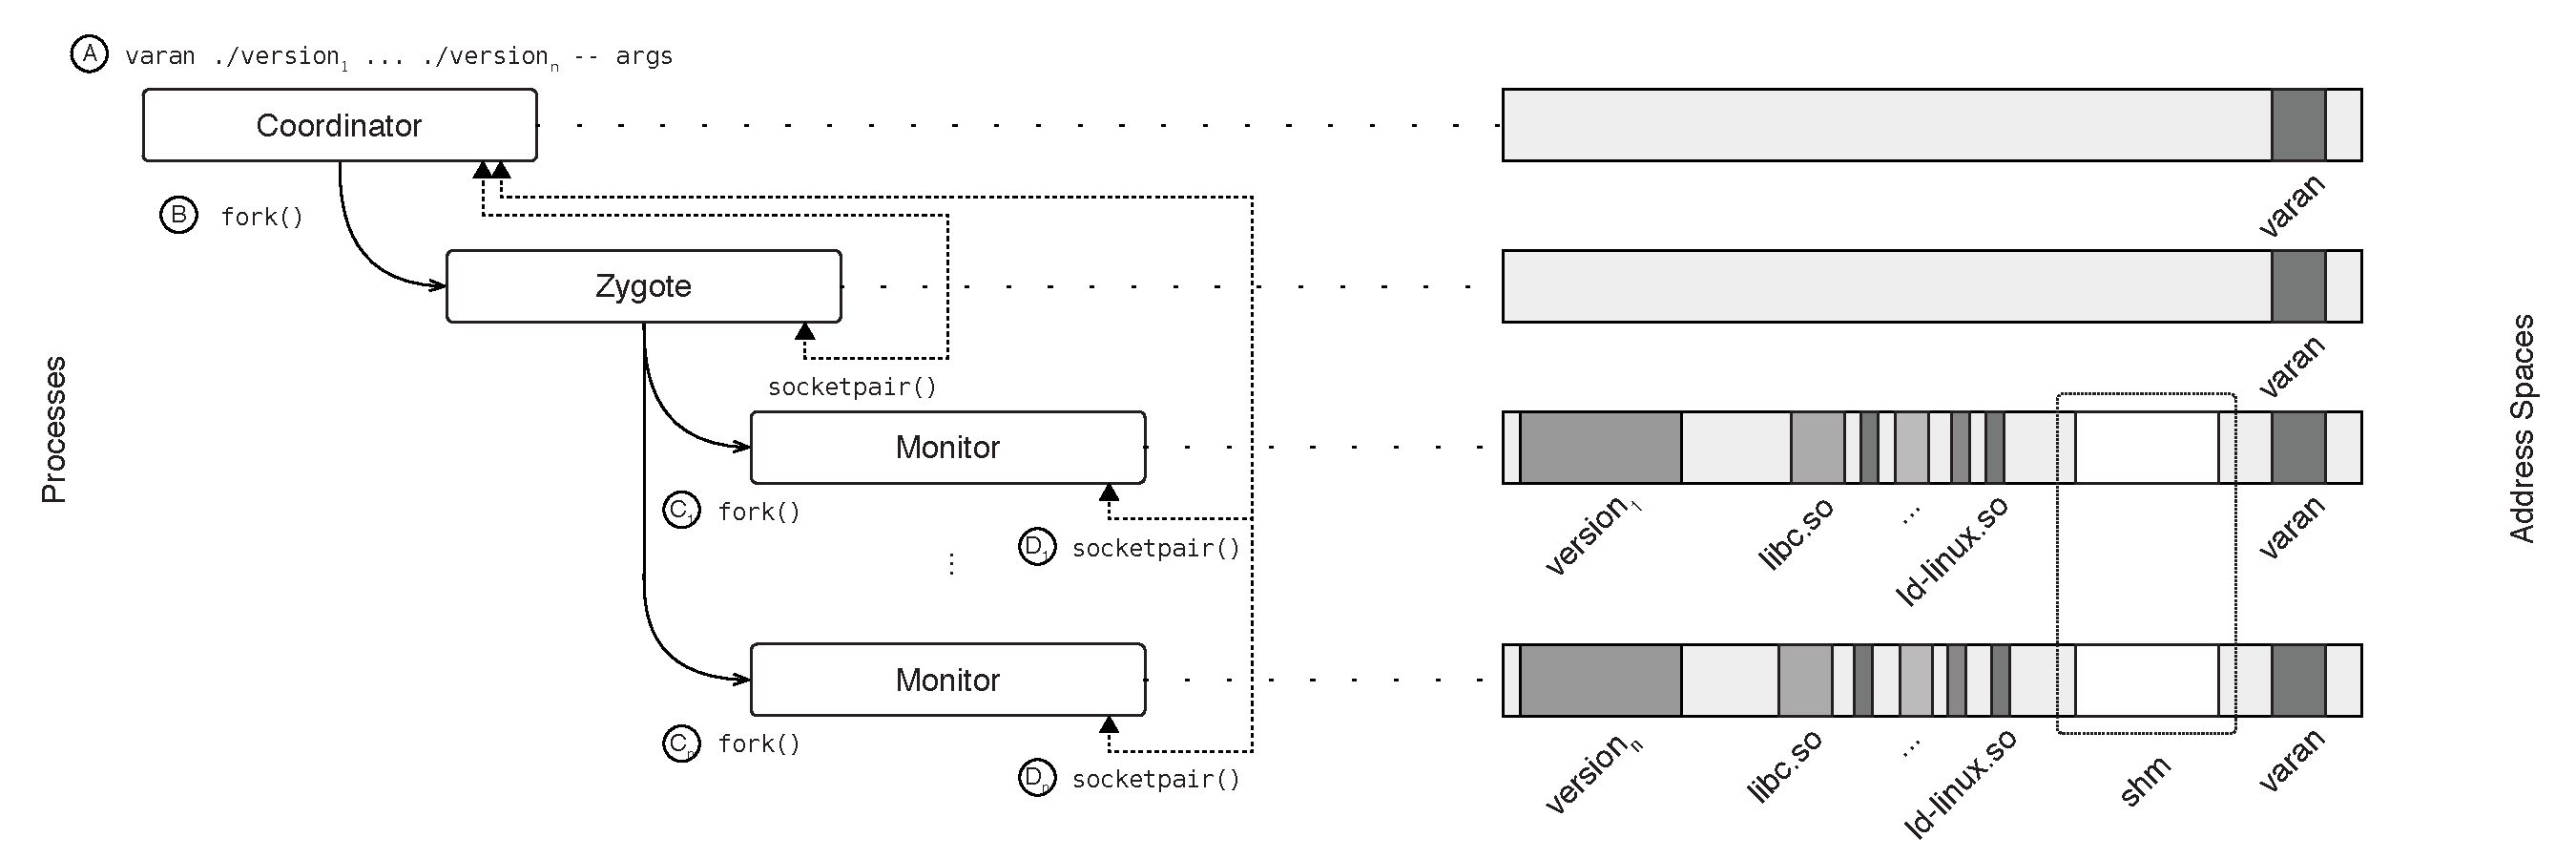
\includegraphics[width=\textwidth]{efficient-execution/figures/address-space}
    \caption{Setup of address spaces and communication channels.}
    \label{fig:setup}
  \end{center}
\end{figure*}


We have implemented our approach in a prototype, to which we will
refer as \vx, targeted at multi-core processors running x86-64 Linux.
\varan works on off-the-shelf binaries (both stripped and unstripped)
and supports single- as well as multi-threaded applications.

When it starts, \vx first sets up the address spaces of all program
versions and establishes the needed communication channels
(\S\ref{sec:setup}).  It then performs selective binary rewriting to
replace all system calls with  jump instructions
(\S\ref{sec:rewriting}).  After these initial stages, the event
streamer component of \vx ensures the coordination of the leader and
its followers (\S\ref{sec:streaming}).


\subsection{Setup of address spaces and communication channels}
\label{sec:setup}

The main steps involved in the setup of version address spaces and the
needed communication channels are shown in Figure~\ref{fig:setup}.  To
run multiple versions in parallel, the user launches \vx providing the
paths to all versions, together with any command line arguments required
to start them (Step \circl{A} in Figure~\ref{fig:setup}). \vx is built
as a statically-linked, position-independent library, to make sure it
does not stand in the way of any segments which have to be loaded by the
application at fixed addresses.

% \begin{lstlisting}[language=bash,numbers=none]
% varan -p /path/to/executable1 
%         -p /path/to/executable2 -- args
% \end{lstlisting}

%The coordinator is linked with the \vx library (\vxlib, stored in
%\stt{libvaran.so}), which will be also injected inside each version.
%\vxlib is built as a statically-linked, position-independent library,
%to make sure it does not stand in the way of any segments which have
%to be loaded by the application at fixed addresses.

The \emph{coordinator} code first creates the shared memory segment
used for communication among versions, and then spawns the
\textit{zygote} process (\circl{B}), which is responsible for starting
the individual versions. The coordinator communicates with the zygote
via a UNIX domain socket. For each version $i$ that needs to be spawned,
the coordinator sends a fork request to the zygote over this socket
pair, which includes the path to that version executable, the command
line arguments, and the end-point of a socket pair which will be used
for the subsequent communication between the coordinator and that
version (\circl{C$_i$}).
%
After receiving this request, the zygote spawns a new process, which
first finalizes the communication with the coordinator
(\circl{D$_i$}).  The coordinator then sends the shared memory
segment descriptor to this process, which maps it inside its address
space.

%% returns a process identifier to the coordinator.  The coordinator then
%% sends the rank and shared memory segment descriptor to the version.

In the final step, the new process starts executing inside the
\emph{monitor} code, which loads the specified ELF executable and sets
up the initial address space as described in the ELF headers. If the
program requires a dynamic linker, \vx loads the linker image specified
in the header as well.
%% Afterwards, \vx attaches the shared memory segment and initializes
%% the system call table based on the rank and arguments provided by
%% the coordinator.
The text segments of both the application and the dynamic linker are
then processed by the binary rewriter (\S\ref{sec:rewriting}). Finally,
\vx jumps to the application entry point as specified in the ELF header,
starting the execution of the application version.

%% \vx is operates at the thin boundary between the operating system and
%% the user-space application---\ie below the C library and the dynamic
%% linker---and lives inside the address space of the host application;
%% however, the application itself is unaware of its existence.

% The rest of this section provides some extra details regarding the
% role and implementation of the coordinator, monitor and zygote.

\boldtext{Coordinator.}  Essentially, to set up the address spaces of
the versions, the coordinator acts as a specialized preloader, inspired
by
\emph{rtldi}.\footnote{\url{http://www.bitwagon.com/rtldi/rtldi.html}}
However, the coordinator does not attempt to replace the existing
dynamic linker, which would be unnecessarily complex and may affect
compatibility with existing applications. Instead, it simply intercepts
system calls performed by the linker to enable the binary rewriter
(discussed in \S\ref{sec:rewriting}) to rewrite the code of
dynamically-linked shared libraries.  One important advantage of our
interception mechanism is that we do not make use of \ptrace to
intercept calls to the dynamic linker---instead, the binary rewriter is
used to rewrite all the system calls done by the linker with jumps into
the coordinator code.  As a result, \vx can be used in combination with
existing \stt{ptrace}-based tools such as \textit{GDB} or
\textit{strace}, which greatly simplifies debugging.

%% This also has an advantage of supporting arbitrary dynamic linkers,
%% not just the one provided by GNU C library, albeit it is going to be
%% the most common target.

%% This architecture has several advantages over other commonly
%% approaches. \vx does not require the use of dynamic linker, as
%% required by \stt{LD\_PRELOAD}. 


\boldtext{Monitor.} To ensure that \vx can be compiled as
statically-linked position-independent code, we must avoid using any
global variables (\ie those in the \stt{.data} section). One of the
consequences is that \vx cannot use any of the existing C libraries such
as \textit{GNU C Library}, as these are not typically built to support
this requirement.  Instead, \vx provides its own implementation of the
necessary C library functions based on the \textit{Bionic C
library}.\footnote{\url{https://android.googlesource.com/platform/bionic.git}}
To support the use of Linux system calls, \vx uses a modified version of
the \stt{linux\_syscall\_support.h}
header.\footnote{\url{https://code.google.com/p/linux-syscall-support/}}

%% \vxlib provides its own entry point (\ie the \stt{\_start} function),
%% which is the starting point for \vx's execution. After start, it first
%% processes the arguments passed on stack by the Linux kernel, including
%% program arguments, environment variables and most importantly the
%% auxiliary data. Then, it loads the specified ELF executable into the
%% address space. Since \vx operates as a pre-loader, it is responsible
%% for setting up the initial address space layout as described by the
%% program header. If the program being executed requires dynamic linker,
%% \vx loads the linker image specified in the program header as
%% well. The text segments of both the application and the dynamic linker
%% are then processed by the binary rewriter (\S\ref{sec:rewriting}).


\boldtext{Zygote.} While it would be technically possible for the coordinator
to create the processes in which versions run, instead of delegating this
functionality onto the zygote, this would bring some complications regarding
the communication channels: for example, the second version spawned would
inherit the communication channel between the first version and the
coordinator, which would be undesirable.  Zygote processes are already used in
popular systems such as \textit{Android} and
\textit{Chrome}~\cite{linuxzygote}---in this paper, we use the term to refer to
the concept rather than a concrete implementation, as \vx provides its own
clean-slate implementation.

After start, \vx sets up the communication subsystem (\ie the shared memory
allocator, the ring buffer) and then forks the Zygote process. The Zygote
closes all open descriptors except for the socket used as a communication
channel with the coordinator and enters the dispatch loop to wait for incoming
requests. On fork request, the Zygote receives command line arguments (\ie
\stt{argv}) and a set of file descriptors which will be available to the new
process; then forks itself and resumes to dispatch loop. The other type of
requests that Zygote supports are querying for process status (\ie equivalent
of \stt{waitpid}) and process termination (\ie \stt{SIGKILL}).

\subsection{Binary Rewriting}
\label{sec:rewriting}

To intercept system calls, \vx uses selective binary rewriting~\cite{bird}.
Unlike traditional dynamic binary rewriting implemented by tools like
DynamoRIO~\cite{dynamorio02} or Pin~\cite{pin05}, where the entire process
image is being rewritten often introducing significant performance overhead,
\vx only replaces certain instructions, in particular the instructions for
performing system calls (\ie \stt{INT 0x80} on x86 and \stt{SYSCALL} on
x86-64).  This approach has been originally implemented in
\emph{BIRD}~\cite{bird} for the Windows/x86 platform and later in
\emph{seccompsandbox}\footnote{\url{https://code.google.com/p/seccompsandbox/}}
for Linux.  Our implementation extends the
\emph{seccompsandbox}\footnote{\url{https://code.google.com/p/seccompsandbox/}}
framework for Linux.

The rewriting itself is done statically when a text segment is mapped into
memory.  (\ie \stt{mmap} system calls with executable flag, typically performed
by the dynamic linker).  \vx iterates through the text segment searching for
system call instructions using a simple x86 disassembler. Every system call
found is rewritten with a jump to an internal system call entry point. This
process is complicated by the fact that while a system call instruction is only
one byte long, a jump instruction requires five bytes. Therefore, in order to
rewrite the system call with a jump, we also need to relocate some of the
instructions surrounding the system call---\ie perform binary detouring via
trampolines~\cite{detours}.  On rare occasions when this is not possible (\eg
because the surrounding instructions are potential branch targets), we replace
the system call with an interrupt (\stt{INT 0x0}).  This interrupt is handled
by \vx through a signal handler installed during initialization, which
redirects the control flow to the system call entry point as for other system
calls.

The system call entry point first saves all registers, and then checks an
internal system call table to see whether there is a handler installed for that
particular system call; if so, it calls that handler (using a user space
calling convention), otherwise it invokes the default handler.  After
processing the system call, the entry point handler restores all registers and
returns to the original caller (using \stt{sigreturn} in the case of system
calls intercepted via an interrupt). The system call entry point also
implements support for restarting system calls, normally handled by the kernel
(\ie signaled by the \stt{-ERESTARTSYS} error code). This is used in certain
scenarios supported by \vx such as transparent failover (\S\ref{sec:failover}).

The internal system call table can be easily changed to accommodate
various application scenarios.  In particular, the only difference
between the leader and the followers is the system call table. For
example, the \stt{write} system call would be redirected in the leader
to a function that performs the call and records its result in the
shared ring buffer, while in the followers it would be redirected to a
function that reads the results from the shared buffer without making
the call.
%% \vx allows both the system call table and the default system call
%% handler to be provided by the embedder of \vx \todo{Where shall we
%%   described the possibility of \vx embedding, \ie building tools on
%%   top of \vx?}. This makes it easy to customize \vx behavior for
%% different use cases (\S\ref{sec:failover}). For our prototype, we have
%% provide three different system call tables (\ie record, replay and
%% passthrough). 
\varan  also provides a Python script which can produce new tables
and their implementations using templates.
%% ; in fact, the passthrough table was implemented using this
%% generator. We have also used the generator throughout the \vx
%% development for testing and debugging purposes.


\subsubsection{Virtual System Calls}
\label{sec:vsyscall}

The \emph{vsyscall} page and the \emph{vDSO} segment are two
mechanisms used to accelerate certain system calls in Linux. Each
process in Linux has two special segments mapped into its address
space, containing virtual system call implementations. These system
calls do not incur the context switch overhead between kernel and
user space associated with "standard" system calls.

The \emph{vsyscall} page was introduced first, but is being deprecated in favor
of the \emph{vDSO} segment.\footnote{We are referring to x86-64 version, on x86
the vDSO segment contains a function used to determine the preferred method of
making a system call} The main reason for this development is that the
\emph{vsyscall} page is mapped to a fixed address, making it susceptible to
return-oriented programming attacks~\cite{ROP:tissec12}. To address this issue,
the vDSO segment is mapped to a random address. Since the segment is
dynamically allocated, it can also support an arbitrary number of virtual
system calls (currently \stt{clock\_gettime}, \stt{getcpu}, \stt{gettimeofday}
and \stt{time}).

Virtual system calls represents one of the major limitations of
\stt{ptrace} based monitors. Since these system calls are entirely
implemented in user space, they cannot be intercepted via \ptrace.
This is an important limitation: as these system calls provide access
to timing information, they are often used as a source of
non-determinism (\eg for random number generators) and their handling
is critical for any NVX system. Despite this, previous systems either
omit discussion on virtual system call handling~\cite{mx,orchestra11}
or explicitly mention their inability to handle them~\cite{tachyon12}.

To our knowledge, \vx is the first NVX system which handles virtual
system calls, using binary rewriting. 
%In \vx, binary rewriting is also used to intercept virtual system
%calls.
Handling calls made via the \textit{vsyscall} page is easier, as
the function symbols are always mapped at the same address.  
We can therefore easily identify calls to these functions while
scanning the text segment and rewrite them to calls into our system
call table.
To handle \textit{vDSO} calls, we first need to
determine the base address of the \textit{vDSO} segment; this address
is passed by the kernel in the ELF auxiliary vector via the
\stt{AT\_SYSINFO\_EHDR}
flag.\footnote{\url{https://www.gnu.org/software/libc/manual/html_node/Auxiliary-Vector.html}}
Second, we need to examine the ELF headers of the \textit{vDSO}
segment to find all symbols.  Since these symbols are allocated at
arbitrary addresses, statically identifying calls to these symbols as
in the \textit{vsyscall} case would be complicated. Instead, we
replace the entry point of each function with a jump to dynamically
generated code which sets up the stack and then issues a call to the
\vx system call entry point as in case of regular system
calls. Furthermore, we provide a trampoline, which allows the
invocation of the original function, by moving the first few
instructions of each function to a new place, followed by a jump to
the original code. This allows \vx to take advantage of the virtual
system call mechanism to further improve performance.

%% Finally, we note that this function interception mechanism is not
%% specific to system calls and can be used to intercept arbitrary
%% functions in the target application if needed, similarly to
%% Detours~\cite{detours}.



\subsection{Event Streaming}
\label{sec:streaming}

As briefly discussed in Section~\ref{sec:overview} and graphically
illustrated in Figure~\ref{fig:architecture}, the leader records all
external events into a shared ring buffer, while the followers replay
them to mimic the leader's behavior.  External events consist
primarily of system call invocations, but also of signals.  The leader
is the only version interacting with the environment, \ie executing
the system calls, with exception of system calls which are local to
the process (\eg \stt{mmap}). % or \stt{sigaction}).

As in any NVX system operating at the level of system calls, \vx has
to be aware of the system call semantics, in order to transfer the
arguments and results of each system call.  \vx currently implements
\syscallsHandlers system call handlers which were specifically selected
to cover the common operations (file and network I/O, event
notification, process management). This has proven enough to
successfully run all applications used in our evaluation.

%, with the remaining system
%calls allowed to be executed directly by each version, which has
%proven enough to successfully run all the servers used in our
%evaluation.

%% All application instances running in parallel under \vx are assigned
%% ranks, similarly to OpenMPI~\cite{OpenMPI}. The instance\footnote{We
%%   refer to the instances rather than a process as application may have
%%   multiple threads/subprocesses} with rank 0 is denoted as
%% \emph{leader} while all other instances are denoted as
%% \emph{followers}. 


%% When followers would execute a system call under normal execution, now
%% they simply return a value from the event stream (\ie the return value
%% of the system call executed by the leader).

% \vx recognizes several different types of events:
% \begin{inparaenum}[(i)]
% \item \emph{syscall} for the system call entry,
% \item \emph{sysret} for the system call exit,
% \item \emph{signal} for an interceptable signal,
% \item \emph{exit} for the process exit.
% \end{inparaenum}
% Furthermore, it is possible to add other types of events if necessary.

%% Each event has a fixed size of 64 bytes where first byte is
%% used as an event type.  The size has been deliberately chosen to be
%% fit into a single cache line on modern x86 CPU (see \S\ref{sec:ipc}
%% for more details).

\subsection{Inter-process Communication}
\label{sec:ipc}

%% \begin{structure}
%% \item Sending events from one process to other without the use of system
%% calls to avoid the additional overhead
%% \item Shared memory queues for process to process communication
%% \item Custom shared memory allocator with reference counting
%% \end{structure}

Since one of our primary goals for \vx was to minimize the performance
overhead, to avoid additional system calls being made during system call
handling (\S\ref{sec:overview}), we have designed an interprocess communication
mechanism which does not use system calls (\eg socket-based communication
primitives).

\subsubsection{Shared ring buffer}
\label{sec:ring}

For fast communication, the leader and its followers share a common
ring buffer of fixed size, which is held entirely in memory.  Our
initial solution used a separate shared queue for each
process~\cite{fastforward,mcringbuffer}, with the
%% Shared memory queues are often used for fast core-to-core
%% communication in high-performance applications.
coordinator acting as an event pump---reading events from the leader's
queue and dispatching them into followers' queues.  This approach
worked well for a low system call rate, but at higher rates the event
pump quickly became a bottleneck.  
% Furthermore, although we used a
% state-of-the-art shared queue implementation~\cite{bqueue}, we still
% experienced a large performance overhead for system call
% interception---over $20\times$ for a worst-case microbenchmark,
% compared to $4\times$ in the final implementation.

As a result, we have instead opted for a design based on Disruptor
pattern~\cite{disruptor} which uses a shared ring buffer allowing concurrent
access by multiple producers and consumers, eliminating the need to dispatch
events among queues, and thus improving both performance and memory
consumption.  Our implementation uses C11 atomics, 
in combination with cache aligning to
achieve maximum performance with minimal use of locking (locks are used only
during memory allocation and deallocation).

The ring buffer is used to stream events between processes. Each event
has a fixed size of 64 bytes; the size has been deliberately chosen to
fit into a single cache line on modern x86 CPUs.  This is sufficient
for sending signals and system calls for which all arguments are
passed by value (on x86-64, a system call can have up to six arguments
of eight bytes, to fit into general purpose registers).  However, for
system call arguments passed by reference, the payload might have
variable size and can be potentially larger than the event itself.  In
this case, we use events to only transfer shared pointers, which
identify memory shared across versions.


\subsubsection{Transferring file descriptors and leader replacement}
\label{sec:leader-repl}

Apart from the ring buffer, each version has a \textit{data channel},
implemented using UNIX domain sockets.
% Together, the ring buffer and data channel form an \emph{event
% stream} which is a primary communication mechanism for exchanging
% events among instances.
The data channel is used to send information which cannot be
transferred via shared memory, in particular open file descriptors.
Whenever the leader obtains new file descriptor (\eg by opening a
file), it sends this descriptor to all followers, effectively
duplicating the descriptor into their processes. This is a crucial
mechanism which enables the leader to be replaced transparently when
it crashes. When the leader crashes, the follower that is elected as
the new leader can simply continue executing using existing
descriptors (\eg responding to requests coming over network) without
any disruption in service.

% Currently, UNIX domain sockets do not support broadcast, so the leader
% communicates with the followers via the coordinator, which then sends
% the descriptor separately to all followers.  However, there are
% proposals to add broadcast support for UNIX domain
% sockets,\footnote{\url{https://lkml.org/lkml/2012/2/20/208}} which would
% simplify the design of our prototype and further improve performance.


\subsubsection{Multi-process and multi-threaded applications}
\label{sec:threading}

Handling threads is crucial in supporting many modern applications. To
alleviate non-determinism issues due to scheduling, \vx enforces
system call ordering across all threads in all variants by using a
single shared ring buffer.  Each event sent through the ring buffer is
annotated with an internal thread ID. When reading events from the buffer, each
thread checks the ID of every new event and blocks if the event ID does not
match its own.  Since our ring buffer implementation (\S\ref{sec:ring}) allows
concurrent writes by multiple producers without the need for expensive
synchronization, the use of a single shared buffer does not hinder the
application performance. 

When a new thread is spawn, a new socket pair is established between the thread
and the coordinator. The leader then continues execution, but the coordinator
waits until all followers spawn a new thread, establishing appropriate socket
pairs for communication, and setting up the thread to read events from the
shared ring buffer.

Our mechanism resembles existing deterministic multi-threading (DMT)
mechanisms~\cite{coredet:asplos10,dthreads:sosp11}. The guarantees
provided by \vx are weaker than those typically provided by these
systems as we do not enforce ordering across atomics-based
synchronization primitives.

The use of a single shared buffer presents a problem when one or more threads
perform a system call which blocks for a long period of time. In such case, the
other threads could run out of space in the ring buffer. Since the ring buffer
uses busy waiting, the following threads would also waste resources. To overcome
this problem, we have introduced a concept of \emph{waitlock}. Whenever the
following thread makes a blocking system calls, it acquires the waitlock. Such
thread is no longer holding a position in the ring buffer and it blocks until it
receives a notification from the leading thread when the waiting thread wakes up
and continues execution. The waitlocks are internally implemented using a
combination of C11 atomics and futexes~\cite{futex} for efficiency.

% However, this weaker form of determinism
% does not typically pose a problem for real-world applications as long
% as they are properly synchronized.  Note that data races resulting
% from missing or incorrect synchronization can cause followers to issue
% a different sequence of system calls from the leader.  If this
% happens, we could either try to apply one of the rewriting rules
% (\S\ref{sec:patternmatching}), or terminate the follower.
%
However, we have not detected any system call divergences caused by
related data races in our benchmarks, which include multi-threaded
applications (\eg \redis), similar to the experience reported for
prior NVX systems.  However, shall this become a problem, we could
address it by employing a stronger form of determinism similar to
existing DMT systems.

%% Each instance also has a dedicated \emph{service channel}, similarly
%% to the data channel implemented using UNIX domain sockets. The service
%% channel is used to transfer commands and service requests between
%% coordinator and the instance.

%% One such example are \stt{fork} and \stt{clone} system calls. The new
%% process spawned as a result of these system calls needs to have its
%% own data and service channel. The parent process is responsible for
%% creating these using a \stt{sockepair} system call. One end of each
%% pair is inherited by the new process while the other end is sent to
%% the coordinator where it is associated with the new process.

%Note that data races resulting from missing or incorrect
%synchronization can cause followers to issue a different sequence of
%system calls from the leader.  If this happens, that follower would
%have to be terminated.  We first note that \vx has not detected any
%system call divergences caused by data races in our benchmarks (which
%include many popular applications such as \apache, \nginx, and \redis),
%so this might not be such an important aspect in practice.  Prior NVX
%systems do not address this problem either, likely due to a comparable
%experience.

%However, we envision two possible solutions.  The first one would be
%to use deterministic multi-threading (\eg
%Dthreads~\cite{dthreads:sosp11}).  The second solution would be to
%allow developers to document any benign races as rewrite rules
%(cf. \S\ref{sec:patternmatching}).

\subsubsection{Memory allocation scheme}  

Efficient shared memory allocation plays an important role in a system
like \vx.  We use a custom shared memory pool allocator
implementation, similar to the one used by
OpenMPI.\footnote{\url{http://www.open-mpi.org/}} The shared memory
allocator uses the notion of buckets for different allocation sizes,
where each bucket holds a list of segments, and each segment is
divided into chunks of the same size; each bucket holds a free list of
chunks.  When there are no more unused chunks in a bucket, the
allocator requests a new segment from the memory pool, and divides it
into chunks which are then added to the free list. Each bucket also
has a lock associated with it which has to be held prior to an
allocation from that bucket. 
% While this design is relatively simple,
% it performed well in our benchmarks. We also experimented with
% more advanced designs (\eg using different allocation strategies for
% smaller and larger blocks), but the basic allocator always
% outperformed all other implementations.  

%% However, we believe it might still be possible to come with a more
%% specialized allocation strategy which would further improve the
%% performance of \vx, and this is something we would like to address in
%% our future work.

%% The critical part of many systems which use shared memory for
%% communication is deallocation. There are various solutions to this
%% problem. One possibility is to use some form of garbage collection,
%% such as reference counting. Unfortunately, this solution is not
%% applicable in our case since the leader is not aware of any of the
%% consumers processing its events making it difficult to consistently
%% manage the reference counts. The original Disruptor implementation,
%% which targets the Java runtime simply relied on the garbage collector
%% provided by the virtual machine. Unfortunately, this solution is not
%% applicable in our case either. Instead, we have extended the C-based
%% Disruptor implementation to notify a follower if it is the last one
%% that processes an event. \todo{how?}  If that is the case, the
%% follower is responsible for freeing the associated memory. This
%% solution does not add any overhead and does not require any
%% modifications to the allocator.

% This property allows us sharing memory between individual application
% instances without explicitly tracking which instance is responsible for
% deallocation, or using the back channel to notify instance that the block is
% available for deallocation as in the case of OpenMPI

\subsection{Rewrite rules for system call sequences}
%\subsubsection{System call filtering and rewriting}
\label{sec:patternmatching}

\vx uses BPF filters to implement the system call rewrite rules introduced in
Section~\ref{sec:rw}.  BPF is a machine language for writing rules and an
interpreter shipped with many UNIX implementations, including Linux and BSD.
BPF filters have been traditionally used to filter network packets, but
recently also for system call filtering as a part of seccomp "mode 2" (also
known as seccomp-bpf).

We have integrated a BPF interpreter in \vx to allow for system call rewrite
rules. Our implementation is based on the Linux kernel code which has been been
ported to user space and extended for NVX execution.  This required adding a
new return value \lstinline`SECCOMP_RET_REPLACE` where the bottom 16-bits of
the return value specify the new system call number the original system call is
going to be rewritten to.  Since these extensions does not add any new
instructions or extend the semantics of the BPF language, the
\lstinline`bpf_asm` tool can be used to compile the filters into a binary form.
This can be then loaded into \vx on start through a command line option.

The use of BPF has a number of advantages.  First, it does not require
the user to modify and recompile the monitor on every rule
change. This is particularly important as rewrite rules are likely
going to be application specific. Second, the BPF machine language was
designed to be simple enough to prevent a large class of errors---\eg
all filters are statically verified on load to ensure termination.
(\ie every filter has to end with a \lstinline`ret` instruction).

We also argue that the choice of BPF as a language for stream rewriting rules
makes it easier to adopt by administrators, the most likely users of \vx,
compared to some other more esoteric languages such as Haskell~\cite{tachyon12}.

\begin{lstlisting}{language=[bpf]Assembler,caption={Example of a BPF rewriting rule}}
ld [0]                /* offsetof(struct seccomp_data, nr) */
jne #1, good          /* __NR_write */
bad: ret #0           /* SECCOMP_RET_KILL */
ldi #18               /* __NR_pwrite */
add #0x00070000       /* 18 + 0x00070000 */
ret %a                /* SECCOMP_RET_REWRITE */
good: ret #0x7fff0000 /* SECCOMP_RET_ALLOW */
\end{lstlisting}

\section{Performance evaluation}
\label{sec:evaluation}

One of the main contributions of \nx is significantly lower
performance overhead compared to the state-of-the-art NVX systems.
Therefore, we have conducted an extensive performance evaluation,
using microbenchmarks (\S\ref{sec:microbenchmarks}), high-performance
C10k servers (\S\ref{sec:c10k}) and servers used to evaluate prior NVX
systems (\S\ref{sec:comparison}).

The microbenchmarks were run on a four-core/eight-thread machine with
a 3.50~GHz Intel Xeon~E3-1280 CPU and 16~GB RAM running 64-bit Ubuntu
14.04 LTS, while the servers were run on a pair of such machines, one
running the server under \nx and the other the client.  The machines
are located in the same rack, connected by a 1~Gb Ethernet.

\subsection{Microbenchmarks}
\label{sec:microbenchmarks}

To measure the overhead introduced by \nx while processing individual
system calls, we designed a series of experiments that compare a
system call intercepted and executed by \nx against the same system
call executed natively. We used five different system calls:

\begin{enumerate}

%\item \stt{close} is representative of an inexpensive system call.
%  We invoke it with argument \stt{-1}, which returns immediately
%  with an error representing a NOP system call.

\item \stt{close(-1)} is representative of an inexpensive system call,
  which returns immediately.

%\item \stt{write} is representative of system calls which involve
%  expensive I/O, but whose result can be sent entirely as a single
%  event in the ring buffer.  We invoke the system call to write a
%  512-byte buffer to \stt{/dev/null}.

\item\stt{write(1 /* /dev/null */, "...", 512)} is representative of system call which involve
  expensive I/O, but whose result can be sent entirely as a single event in the
  ring buffer.

%\item \stt{read} is representative of system calls which involve
%  expensive I/O, and whose result cannot be fully included in the
%  associated event in the ring buffer.  Instead, it has to be copied
%  via additional shared memory (\S\ref{sec:ring}). We invoke the
%  system call to read a 512-byte buffer from \stt{/dev/zero}.

\item \stt{read(0 /* /dev/null */, "...", 512)} is representative of system calls which
  involve expensive I/O, and whose result cannot be fully included in the
  associated event in the ring buffer.  Instead, it has to be copied via
  additional shared memory (\S\ref{sec:ring}).

%\item \stt{open} is representative of system calls that require
%  transferring file descriptors (\S\ref{sec:leader-repl}).  We invoke
%  it with \stt{/dev/null} and \stt{O\_RDONLY} as arguments.

\item \stt{open("/dev/null", O\_RDONLY)} is representative of system calls that
  require transferring file descriptors (\S\ref{sec:leader-repl}).

\item \stt{time(NULL)} is a virtual system call implemented via the
  \textit{vDSO} segment (\S\ref{sec:vsyscall}). It internally calls
  \stt{\_\_vdso\_time} (since glibc 2.15).  We could not measure
  the overhead of using the \textit{vsyscall} page, because it is
  deprecated on our system (and all recent versions of Linux), with
  all \textit{vsyscalls} now redirected to their \textit{syscall}
  versions.

\end{enumerate}

%% The \stt{open} demonstrates the cost of the file descriptor transfer; we have
%% used the \stt{/dev/null} file with \stt{O\_RDONLY} flag. \stt{read} and
%% \stt{write} use the I/O performance overhead, by reading and writing 512B
%% buffer from \stt{/dev/zero} and to \stt{/dev/null} respectively. The \stt{read}
%% is clearly more expensive system call, as it needs to transfer the content of
%% the buffer read using the shared memory (\S\ref{sec:streaming}). The
%% \stt{close} system call is a representative of all other cases.

We execute each system call one million times and compute the average
of all execution times.  Time measurements were done using the time
stamp counter (\ie the \stt{RDTSC} instruction). Each set of
measurements was preceded by a warm-up stage in which we executed the
system call $10,000$ times. % to warm up the caches.

\begin{figure}[!t]
  \centering
  \includegraphics[width=\columnwidth]{efficient-execution/graphs/micro.pdf}
  \caption{System call microbenchmarks.}
  \label{fig:micro_syscall}
\end{figure}

%\begin{figure}[!t]
%  \centering
%  \includegraphics[width=\columnwidth]{efficient-execution/graphs/micro_syscall.pdf}
%  \caption{System call microbenchmarks.}
%  \label{fig:micro_syscall}
%\end{figure}

Figure~\ref{fig:micro_syscall} shows the results.  The first set of bars
labeled \textit{native} shows the execution time without \nx.  The second set
of bars labeled \textit{intercept} shows the execution time with interception
measuring the cost of binary rewriting: for taking these measurements, the
intercepted system call is immediately executed, without any additional
processing.  As it can be seen, the interception cost is small, at under
\maxInterceptOvh in all cases. The overhead of intercepting the virtual system
calls is high in relative terms, but low in absolute ones: \vdsoIntercept vs
\vdsoNative for native execution in case of \stt{time}.

The set of bars labeled \textit{leader} shows the execution time of each
system call being interecepted, executed and recorded by the leader.
That is, it is the sum of the \textit{intercept} cost and the
cost of recording the system call.  For \stt{close} and \stt{write},
the overhead is only \closeLeaderOvh and \writeLeaderOvh respectively on top of
the native execution, because the arguments and results of these system calls
can be recorded in a single event.  For \stt{read}, this is more expensive, at
139\%, because transferring the result also involves accessing additional
shared memory.  Finally, the cost for \stt{open} is the highest, since it also
involves the slower transfer of the returned file descriptor via a UNIX domain
socket.

Finally, the set of bars labeled \textit{follower} shows the execution time
incurred by the follower which has to intercept each system call and read its
results from the ring buffer and (if necessary) shared memory.  As expected, the
costs for \stt{close} and \stt{write} are low (and significantly lower
than executing the system call), because the entire result fits into a
single event on the ring buffer. The costs for \stt{read} and
\stt{open} are again higher, because they involve additional shared
memory and transferring a file descriptor, respectively, but they are
still lower than the costs incurred by the leader.


%\boldtext{vDSO calls.}  We similarly measured the overhead of
%performing a virtual system call via the \textit{vDSO} segment
%(\S\ref{sec:vsyscall}).  The system call used was \stt{time},
%which internally calls \stt{\_\_vdso\_time} (since \stt{glibc
%  2.15}).  We could not measure the overhead of using the
%\textit{vsyscall} page, because it is deprecated on our system (and
%all recent versions of Linux), with all \textit{vsyscalls} now
%redirected to their \textit{syscall} versions.

%\begin{figure}[!t]
%  \centering
%  \includegraphics[width=\columnwidth]{efficient-execution/graphs/micro_vsyscall.pdf}
%  \caption{vsyscall and vDSO microbenchmarks.}
%  \label{fig:micro_vsyscall}
%\end{figure}

%Figure~\ref{fig:micro_syscall} shows the results, using the same set
%of bars as in Figure~\ref{fig:micro_syscall}.  We have opted this time
%to show absolute numbers, and to include the data for \stt{close(-1)}
%from Figure~\ref{fig:micro_syscall} for comparison.  The overhead of
%intercepting the system call is high in relative terms, but low in
%absolute ones: \vdsoIntercept vs \vdsoNative for native execution.
%The \textit{leader} and \textit{follower} costs are similarly high in
%relative terms but low in absolute ones: \vdsoLeader and
%\vdsoFollower, respectively.

\subsection{C10k servers}
\label{sec:c10k}

Existing NVX systems, including those based on \lstinline`ptrace`, can
already run CPU-bound applications efficiently with an overhead
typically less than \SI{20}{\percent}.  As a result, we focus our evaluation on
high-performance, heavily I/O-bound C10k servers\footnote{Numeronym used
  for servers capable of concurrently handling ten thousand connections.}
  which%
\begin{inparaenum}[(1)]
\item represent the worst-case scenario for a system call monitor; and
\item form the backbone of modern, highly-scalable web applications,
  for which reliability is critical.
\end{inparaenum}

The \nservers server applications used in our evaluations are
summarized in Table~\ref{tbl:apps} (the size is measured in lines of
code, as reported by the \emph{cloc} tool). For our performance experiments, we
ran the same version of each application multiple times with different number
of instances. 
%(in practice you would typically run different versions as shown in \S\ref{sec:applications}).  
Each experiment was performed six times, with
the first measurement used to warm up the caches and discarded.  The overhead
was calculated as a median of the remaining five measurements.

\begin{table}
\begin{center}
\caption{Server applications used in the evaluation.}
\begin{tabular}{lrl}
  \toprule
  \textsc{Application} & \textsc{Size} & \textsc{Threading} \\
  \midrule
  Beanstalkd & 6365 & single-threaded \\
  Lighttpd & 38,590 & single-threaded\\
  Lighttpd 2.0 & 47,873 & multi-threaded\\
  Memcached & 9779 &  multi-threaded\\
  Nginx & 101,852 & multi-process\\
  Redis & 34,625 & multi-threaded\\
  \bottomrule
\end{tabular}
\end{center}
\label{tbl:apps}
\end{table}

% \begin{figure}[!t]
%   \centering
%   \includegraphics[width=\columnwidth]{results/macro}
%   \caption{Performance overhead for the \beanstalkd, \lighttpd and \nginx servers for different number of followers.}
%   \label{fig:servers}
% \end{figure}

% \begin{figure*}[!t]
%  \centering
%  \includegraphics[width=0.6\textwidth]{results/c10k}
%  \caption{Performance overhead for the \beanstalkd, \lighttpd and \nginx servers for different number of followers.}
%  \label{fig:servers}
% \end{figure*}

% \begin{figure*}[!t]
%  \centering
%  \includegraphics[width=0.6\textwidth]{results/macro_redis}
%  \caption{Performance overhead for \redis operations for different number of followers.}
%  \label{fig:redis}
% \end{figure*}

\begin{figure}[!t]
 \centering
 \includegraphics[width=\textwidth]{efficient-execution/graphs/c10k}
 \caption{Performance overhead for the \beanstalkd, \lighttpd, \nginx
   and \redis servers for different number of followers.  The client
   and server are located on the same rack, simulating a worst-case scenario.}
 \label{fig:servers}
\end{figure}

We give a short overview of each benchmark and the way in which we
measure performance (namely throughput) in our experiments:

\paragraph{\beanstalkd}\footnote{\url{http://kr.github.io/beanstalkd/}}
is a simple and fast work queue, used by a number of websites to
distribute jobs among workers. We used revision \lstinline`157d88b` from the
official \git repository, the latest revision at the time of
writing.  To measure performance, we used
\lstinline`beanstalkd-benchmark`\footnote{\url{https://github.com/fangli/beanstalkd-benchmark}}
with \num{10} concurrent workers each performing \num{10000} push operations
using \SI{256}{\byte} of data per operation.

%\boldtext{\textit{Lighttpd}}\footnote{\url{http://www.lighttpd.net/}}
%is a lightweight web server optimized for high performance
%environments. The version used for the measurements was 1.4.36,
%the latest version in the 1.4.x series at the time of writing.
%We measured the performance of serving a \SI{4}{\kilo\byte} page using
%\lstinline`wrk`, which was run for \SI{10}{\second} with \num{10} clients.

\paragraph{\lighttpdtwo}\footnote{\url{https://github.com/lighttpd/lighttpd2}}
is a lightweight web server optimized for high performance environments,
reimplemented entirely from the scratch in the version 2.0.  We used the
revision \lstinline`93d04a3` from the official \git repository, the
latest revision at the time of writing. We measured the performance of serving
a \SI{4}{\kilo\byte} page using
\lstinline`wrk`,\footnote{\url{https://github.com/wg/wrk}}, which was run for
\SI{10}{\second} with \num{10} clients.

%% \lstinline`weighttpd`\footnote{\url{https://github.com/lighttpd/weighttp}},
%% which is the benchmarking tool developed by the authors of
%% \lighttpd. We set up \lstinline`weighttpd` to perform \num{100,000} requests,
%% using \num{10} concurrent clients running in \num{2} threads.
%The results can be seen in Figure~\ref{fig:macro_lighttpd}.

\paragraph{\memcached}\footnote{\url{http://memcached.org/}} 
is a high-performance, distributed memory object caching system, used by
many high-profile websites to alleviate database load. We used the
revision 1.4.17, latest at the time of writing. To measure the performance
overhead, we used the \emph{memslap} benchmark,\footnote{url{http://libmemcached.org/}}
part of the \emph{libMemcached} library. We used the default workload,
\ie initial load of \num{10000} key pairs and \num{10000} test executions.

%% To measure the performance overhead introduced by \varan when running
%% \memcached, we used \lstinline`memslap`, a load generation and benchmarking
%% tool for \memcached, which is a part of
%% \lstinline`libmemcached`.\footnote{\url{http://libmemcached.org/}}

\paragraph{\nginx}\footnote{\url{http://nginx.org/}}
is a highly popular reverse proxy server often used as an HTTP web
server, load balancer or cache. We used version 1.5.12, the
latest at the time of writing.  We measured
performance using the same workload as for \lighttpdtwo.

%% measured the performance of serving
%% a simple HTML webpage using
%% \lstinline`wrk`,\footnote{\url{https://github.com/wg/wrk}} which was run for
%% \SI{10}{\second} with \num{10} clients.

\paragraph{\redis}\footnote{\url{http://redis.io/}}
is a high-performance in-memory, key-value data store, used by many
well-known services. % such as Twitter, GitHub and StackOverflow.
% Pinterest, Snapchat, Craigslist, Digg, Flickr 
We used version 2.9.11 in our experiments.  To measure
performance, we used
\emph{redis-benchmark},\footnote{\url{http://redis.io/topics/benchmarks}}
distributed as part of Redis. The benchmark issues different types
of commands supported by Redis and measures both the throughput and
the latency for each type. We used the default workload, \ie 50
clients issuing \num{10000} requests and calculated and average overhead
across all commands. 

Figure~\ref{fig:servers} shows the results for all servers. All
performance numbers are obtained using the client-side tools presented
above.  Since the client machine is located on the same rack as the
server, these numbers represent a worst-case scenario, as the network
latency would hide some of the overhead for a more distant client
machine.

%Figures~\ref{fig:servers} and \ref{fig:redis} show the results for all
%servers.  The results for \redis are shown separately, because \redis
%has 16 different command types.  All performance numbers are obtained
%using the client-side tools presented above.  Since the client machine
%is located on the same rack as the server, these numbers represent a
%worst-case scenario, as the network latency would hide some of the
%overhead for a more distant client machine.

For each benchmark, we show one bar, normalized relative to native
execution, showing the performance of \varan using a given number of
followers.  We stop at six followers, because our machine has eight
threads, and we also need one thread for the leader and one for the
coordinator.  
%For space reasons, for \redis we show results for only 0, 3 and 6 followers.

The set of bars for 0 followers measure the interception overhead
of \varan using binary rewriting.  This overhead is negligible for
\lighttpd, \memcached and most \redis operations, \nginxIntercept for \nginx,
and \beanstalkdIntercept for \beanstalkd.

For all benchmarks, we see that the performance overhead increases
slightly with the number of followers.  For instance, the overhead for
\beanstalkd increases from \beanstalkdOneFollower for one follower to
\beanstalkdSixFollowers for six followers, while the overhead for
\lighttpd increases from \lighttpdOneFollower to
\lighttpdSixFollowers.

The figure also shows that there is a significant difference across
benchmarks: the worst performer is \beanstalkd, which sees performance
degradations in the range of \SIrange{55}{81}{\percent}, while the best performers are
\lighttpd, with only \SIrange{12}{15}{\percent} overhead and some operations in \redis
(not shown separately in Figure~\ref{fig:servers})
%such as \lstinline`LRANGE_300`, \lstinline`LRANGE_500` and \lstinline`LRANGE_600`
with under \SI{3}{\percent} overhead.


\subsection{Comparison with prior NVX systems}
\label{sec:comparison}

While Sections~\ref{sec:microbenchmarks} and \ref{sec:c10k} illustrate the
worst-case synthetic and real-world scenarios for a system call monitor, in
order to compare \varan directly with prior NVX systems, we have also run it on
the same set of benchmarks used to evaluate prior systems.  In particular, we
chose to compare against two state-of-the-art NVX systems:
%\strata~\cite{cox2006}, \orchestra~\cite{orchestra09}, and
\tachyon~\cite{tachyon12}.  These systems and their benchmarks are briefly
described  in the first three columns of Table~\ref{tbl:systems}.  To our
knowledge, we are the first to perform an extensive performance comparison of
existing NVX systems.

\begin{table*}[t]
\begin{center}
\caption{Existing systems we have compared \varan against.}
\label{tbl:systems}
\begin{tabular}{lllrr}
  \toprule
  \textsc{System} & \textsc{Mechanism} & \textsc{Benchmarks} & \textsc{Overhead} & \textsc{\varan} \\

  \midrule
  \mx~\cite{mx} & ptrace & \lighttpd (http\_load) & \mxLighttpd & \lighttpdHttploadOneFollower \\
                      &  & \redis (redis-benchmark) & \mxRedis & \redisOneFollower \\
                      &  & \speczerosix & \mxSpec & \speczerosixOneFollower \\
  %\hline
  %\strata~\cite{cox2006} & modified kernel & \httpd (WebBench 5.0) & \strataHttpd & \httpdWebBenchOneFollower  \\
  \hline
  \orchestra~\cite{orchestra09} & ptrace & \httpd (ApacheBench)    & \orchestraHttpd & \httpdAbOneFollower  \\
                                &        & \speczerozero & \orchestraSpec & \speczerozeroOneFollower \\
  \hline
  \tachyon~\cite{tachyon12} & ptrace & \lighttpd (ApacheBench) & \tachyonLighttpd & \lighttpdAbOneFollower \\
                            & & \thttpd (ApacheBench) & \tachyonThttpd & \thttpdOneFollower \\
  \bottomrule
\end{tabular}
\end{center}
\end{table*}

\begin{figure}[!t]
 \centering
 \includegraphics[width=\textwidth]{efficient-execution/graphs/comparison}
 \caption{Performance overhead for the \httpd, \thttpd, and \lighttpd
   servers for different numbers of followers to allow for comparison
   with existing systems.}
 \label{fig:comparison}
\end{figure}


The last two columns of Table~\ref{tbl:systems} show the cumulative
results.  Since prior systems only handle two versions, the comparison
is done against \varan configured in the same way.  However, we remind
the reader that one of the strengths of \varan's decentralised
architecture is that it can often handle multiple versions with minimum
additional overhead, and below we also show how \varan performs on
these benchmarks when more than two versions are used.

\paragraph{\httpd} \footnote{\url{https://httpd.apache.org/}}
was used by \orchestra.  We used version 1.3.29, the same as in the
original work~\cite{orchestra09}.  The overhead reported for
\orchestra is \orchestraHttpd using the \emph{ApacheBench}
benchmark. \varan introduces \httpdAbOneFollower overhead using the
same benchmark, which is a significant improvement.
Figure~\ref{fig:comparison} shows the overhead introduced by \varan
for \httpd (and the other servers used to evaluate prior work) with
different numbers of followers.  As it can be seen, \varan scales very
well with increasing numbers of followers for these benchmarks.

%was used by both \strata and \orchestra.  We used version 1.3.29
%mentioned by \orchestra (\strata did not report the version used).
%The overhead reported for \orchestra is \orchestraHttpd using the
%\emph{ApacheBench} benchmark and \strataHttpd for \strata using
%\emph{WebBench 5.0}. \varan introduces \httpdWebBenchOneFollower overhead
%using \emph{WebBench} and \httpdAbOneFollower overhead with
%\emph{ApacheBench}, which is an improvement over previous work.

\paragraph{\lighttpd} %\footnote{\url{http://www.lighttpd.net/}}
has been used to evaluate both \mx and \tachyon.  We used version
1.4.36. %(neither \mx nor \tachyon reported the version used). 
\mx used the \emph{http\_load} benchmark and reported \mxLighttpd overhead
while \tachyon used the \emph{ApacheBench} benchmark and reported a
\tachyonLighttpd overhead.  When benchmarked using \emph{http\_load},
\varan introduced only \lighttpdHttploadOneFollower overhead, while with
\emph{ApacheBench} it introduced no noticeable
overhead. %\lighttpdAbOneFollower.  
In both
cases, this marks a significant improvement over previous work.

\paragraph{\thttpd}\footnote{\url{http://www.acme.com/software/thttpd/}}
was shown to introduce \tachyonThttpd overhead when run on top of
\tachyon using the \emph{ApacheBench} benchmark. When run on top of
\varan using the same settings as in \cite{tachyon12}, we have not
measured any noticeable overhead.

\paragraph{\redis} 1.3.8 \footnote{\url{http://redis.io/}}
was used in the evaluation of \mx.  The performance
overhead reported by \mx was \mxRedis using the \lstinline`redis-benchmark`
utility. When run with \varan using the same benchmark and the same workload,
the overhead we measured was \redisOneFollower, which is again a significant
improvement over previous work.

\begin{figure*}[!t]
  \centering
  \includegraphics[width=\textwidth]{efficient-execution/graphs/spec2000}
  \caption{\speczerozero performance overhead for different numbers of followers.}
  \label{fig:spec2000}
\end{figure*}

\paragraph{\speczerozero}\footnote{\url{http://www.spec.org/cpu2000/}} 
was used to evaluate \orchestra.  We used the latest available version
1.3.1.  \orchestra reported a \orchestraSpec overhead, while \varan
introduced only a \speczerozeroOneFollower overhead. The results for
the individual applications contained in the \speczerozero suite and
for different numbers of followers can be seen in
Figure~\ref{fig:spec2000}. The reason these applications scale poorly
with the number of followers is likely due to memory pressure and
caching effects~\cite{jaleel07}, and to the fact that our machine has
only four physical cores (with two logical cores each).  We plan to
investigate these results in more detail in future work.

\begin{figure*}[!t]
  \centering
  \includegraphics[width=\textwidth]{efficient-execution/graphs/spec2006}
  \caption{\speczerosix performance overhead for different numbers of followers.}
  \label{fig:spec2006}
\end{figure*}

\paragraph{\speczerosix}\footnote{\url{http://www.spec.org/cpu2006/}}
was previously used to evaluate \mx. We used the latest version 1.2.  The
overhead reported by \mx was \mxSpec, while \varan introduced only
a \speczerosixOneFollower overhead.
Individual results can be seen in Figure~\ref{fig:spec2006}.  


%\begin{figure}[!t]
  %\centering
  %\includegraphics[width=\columnwidth]{results/macro_beanstalkd}
  %\caption{Beanstalkd performance overhead.}
  %\label{fig:macro_beanstalkd}
%\end{figure}

%\begin{figure}[!t]
  %\centering
  %\includegraphics[width=\columnwidth]{results/macro_lighttpd}
  %\caption{Lighttpd performance overhead.}




%\section{Challenges}
%\subsection{System call interception}
%\subsection{Event-based architecture}
%\subsection{System call rewriting}

%\chapter{\nx prototype system}

%\section{Address space setup}
%\section{Communication channels}
%\section{Binary rewriting}
%\subsection{System calls}
%\subsection{Virtual system calls}
%\subsection{Function calls}
%\section{Event streaming}
%\subsection{Interprocess communication}
%\subsection{Shared ring buffer}
%\section{Handling non-determinism}
%\subsection{Multi-process and multi-threaded applications}
%\subsection{Rewrite rules for system calls}

%\chapter{Performance Evaluation}
%\label{chap:performance-evaluation}

%\section{Microbenchmarks}
%\section{Macrobenchmarks}
%\section{Comparison with prior NVX systems}


\chapter{Other applications}
\label{chap:applications}

\nx is designed as a flexible framework that can support a variety of
application scenarios involving NVX systems.  In this section, we
discuss three such scenarios:  transparent failover
(\S\ref{sec:failover}), live sanitization
(\S\ref{sec:sanitization}), and record-replay
(\S\ref{sec:record_replay}).

% \subsubsection{Regression Testing}
% \label{sec:testing}

% One of the most obvious applications of \nx framework is regression testing.
% Developers often made various assumption about their programs. When working on
% a new version, regression testing is often used to ensure that these
% assumptions still hold even in the new version. Unfortunately, testing is not
% an exhaustive technique and since regression tests are often written by the
% same developers as the software itself, there is a high probability that some
% violations will be violated leading to security bugs~\todo{Give concrete
% examples.}.

% Executing the regression suite under \nx while running both versions in
% parallel (possibly even more) might help to reveal the subtle differences,
% otherwise undetected by the tests. Our current prototype can be instructed to
% stop the application when a divergence in the event stream is discovered
% providing a detailed information of the difference (\eg system call and its
% arguments). \nx may also attempt to continue execution performing different
% system calls. However, this may not always be possible (\eg in case of network
% communication), see discussion in \ref{sec:patternmatching} for more details.


%The results are summarized in Figure~\ref{fig:scribe_vs_nx}.

%% \begin{figure}[t]
%%   \begin{center}
%%     \caption{Performance comparison.}
%%     \label{fig:scribe_vs_nx}
%%   \end{center}
%% \end{figure}

\section{Multi-variant execution}
\label{sec:multi-variant}

%% \begin{structure}
%% \item Rewriting rules for system call patterns
%% \end{structure}

Multiple different variants of the same software version can be run inside an
NVX system as long as they all issue the same sequence of system
calls~\cite{mx}.  This limitation is due to the fact that prior NVX systems run
versions in lockstep (\S\ref{sec:coordination}).

%While software patches often do not affect the sequence of system
%calls, there are however situations when this happens.  In particular,
%many divergences in system call traces fall into the following two
%categories:

%\begin{description}
  %\item[Addition/removal] This class characterizes situations when one
    %of the versions performs an additional system call (or conversely
    %does not perform), typically as a consequence of an additional
    %check.
  %\item[Coalescing] This class covers the situations when a (repeated)
    %sequence of system calls is executed a different number of times
    %in each version.  E.g., one version might execute two \stt{write}
    %system calls, while another a single equivalent \stt{write} to
    %write the same bytes (\eg because extra buffering is used).  
%\end{description}

%Because \nx does not run the versions in lockstep, it can provide the
%ability to handle these two cases.  To illustrate, we ran together
%\lighttpd revision \stt{2436} together with the following revision
%\stt{2437}, which introduced two extra checks using the system calls
%\stt{getuid} and \stt{getgid}.  We configured \nx to allow followers to
%skip these calls, or conversely to execute them if they are not found
%in the event stream.  After these calls, execution was able to continue
%as expected, with both versions issuing the same system calls.  In
%future work, we plan to explore a more general mechanism for writing
%such \textit{rewrite rules} using BPF filters.


%To handle various instances of these classes, we introduced an approach
%based on pattern matching. The pattern language employed by \nx is
%similar to regular expressions, but rather than instances of strings, it
%is used to match instances of system call traces. We have employed
%regular language which allows us to construct a non-deterministic finite
%automaton for each pattern using the technique introduced by Ken
%Thompson~\cite{regexp}.

%The pattern language employed by also \nx allows to match system call
%arguments, similarly to BPF filters in mode 2 seccomp provided by Linux
%kernel, which is necessary to match certain traces.



% and restarts the last system call.  All other followers simply discard
% the event and continue in execution.

% and then notifies all versions by issuing a special
% "reranking" event and sends new ranks to all instances over the
% service channel. When the event is read by individual followers during
% replay, they receive their new ranks and take the action. 


% \todo{Memory consumption?}

% \begin{structure}
% \item Scaling w/ more versions/variants
% \item Fail-over mechanism w/ many versions/variants
% \item Multiple versions: \mx, staged deployment
% \item Variants: sanitizers? some memory allocation diffs?
% \item different compilers?  gcc vs llvm?
% \item sanitizers?
% \end{structure}



\section{Honeypots}

\section{Transparent Failover}
\label{sec:failover}

%[Cite \cite{rx,fo,mx}]

NVX systems introduce a variety of opportunities for increasing
software reliability and availability via transparent failover.  For
instance, one can run in parallel multiple variants of an application with
different memory layouts, different software revisions or different
implementations of a given interface to survive bugs that occur 
only in some of them.   

\nx makes it easy to implement transparent failover.  When one of the
versions crashes, the \stt{SIGSEGV} signal handler installed in each
version notifies the coordinator, which decides what restart strategy
to use.  When one of the followers crashes, it unsubscribes it from
the list of currently-running followers, and discards it without
affecting other followers.  When the leader crashes, it designates one
of the followers as the new leader (currently the one with the
smallest internal ID), and notifies it to switch its system call table
(\S\ref{sec:rewriting}) to that of the leader, and to restart the last
system call while discarding the old (crashing) leader.

To demonstrate support for transparent failover, we used the same scenario as
the one used in evaluation of Mx~\cite{mx}; we ran in parallel two revisions of
\redis, \stt{a71f072f} and \stt{7fb16bac}, the latter of which had a known
crash bug.  We then set up a client to send an \stt{HMGET} command that
triggers the bug, and measured the increase in latency for that command.  When
the buggy version is a follower, we do not observe any increase in latency, as
expected.  When the buggy version is a leader, the latency increases from
\redisnormallatency to \redisfailoverlatency.  As expected, we observed no
extra degradation in throughput for the commands that follow.

\section{Live Sanitization}
\label{sec:sanitization}

Sanitization is one of the most effective testing techniques for
revealing low-level bugs such as uninitialized pointer dereferences and
use-after-free errors.  Both Clang and GNU C Compiler now include a set
of sanitizers---AddressSanitizer (ASan), MemorySanitizer (MSan),
ThreadSanitizer (TSan)---which can be used to statically instrument
the code with various checks.  Unfortunately, these checks introduce
extra overhead (\eg $~2\times$ for ASan, $~3\times$ for MSan and
$~5$-$15\times$ for TSan).  which is why these sanitizers are typically
only used in off-line testing. However, during testing developers only
use a limited set of inputs which might not reveal all bugs.

One possible solution is to record execution traces during deployment
and then replay them in a testing environment with sanitization
enabled. However, this approach is unlikely to work in practice for
several reasons. First, since we do not know in advance which traces
are potentially interesting (\eg trigger sanitization checks) and
which are not, we have to potentially collect and replay a huge number
of execution traces. Even with some form of deduplication, this is
still often impractical. Second, for long running applications such as
servers, the log size will quickly grow to a large size. Third, many
customers will refuse to share the logs from their production
deployment.
% While we may attempt to anonymize these logs, this could
% potentially hide interesting cases.

With \nx, we can perform live sanitization by running the native
unsanitized version as the leader, with sanitized versions as
followers. While sanitization itself introduces a performance
overhead, since followers do not need to execute any I/O operations
and merely replay them, they often can keep up with the follower thus
allowing users to run sanitized versions in production without
introducing any significant overhead.

To demonstrate this, we build revision \stt{7f77235} of \redis twice:
once with Clang without any sanitization, once with ASan enabled.  We
then ran both versions in parallel using \varan and used the same
benchmark with the same settings as for our performance evaluation
(\S\ref{sec:c10k}). As expected, we have not measured any slowdown
compared to the scenario with two non-sanitized versions being run in
parallel. To get a better insight into the effect of running the
sanitized version with \varan, we have measured the median length of
the log, \ie the distance between the leader and the follower. With
sanitization, this length increases from
\redisNoSanitizationMedianLength to \redisSanitizationMedianLength,
which does not impose any problems (\varan uses a default ring buffer
size of 64k events).

\section{Record-Replay}
\label{sec:record_replay}

Although \nx shares similarities with record-replay systems, there are
significant differences; in particular, the log is of fixed size and
only kept in-memory.  However, it is possible to easily extend \nx to
provide full record-replay capabilities by implementing two artificial
clients:
\begin{inparaenum}[(i)]
\item one acting as a \emph{follower} whose only goal is to write the
  content of the ring buffer to persistent storage, and
\item one acting as a \emph{leader}, reading the content of the log
  from the persistent storage and publishing events into the ring
  buffer for consumption by other clients.
\end{inparaenum}

Compared to some of the previous record-replay systems, \varan has a
number of advantages. First, decoupling the logic responsible for
reading/writing the log from the actual application into a separate
process allows the application to run at nearly full speed and utilize
the multiple cores available in modern CPUs.  Second, since \nx was
designed to run multiple instances at the same time, we can replay
multiple versions at once, \eg to determine which versions of the
application from a given range are susceptible to a crash reported by
the user.

We have implemented a simple prototype of the two aforementioned
clients on top of \nx and compared its performance against
\scribe~\cite{scribe}, a state-of-the-art record-replay system
implemented in the kernel.  Unfortunately, because \scribe is
implemented in the kernel and is only maintained for an old 32-bit
Linux kernel (2.6.35), we had to run our experiments inside a virtual
machine (provided by \scribe's authors as the source tree was broken
at the time of our experiments). This experience clearly shows one of
the main disadvantages of kernel-level frameworks---the difficulty of
maintaining the code base. To allow for more faithfull comparison we
ran \nx inside the same virtual machine.

We used \redis as a benchmark, running the same workload as before,
and configured both systems to record the execution to
persistent storage.  We recorded an overhead of \redisRROvhScribe for
\scribe,\footnote{The overhead we measured for \scribe
is higher than overhead reported in~\cite{scribe}; however, please keep in
mind that the original work used less aggressive benchmarks such as \httpd.
The use of a virtual machine may have also affected the result.}
compared to \redisRROvhNx for \nx.
%(but remember that we ran it inside a virtual machine)

% Despite being implemented in the kernel, \scribe
% performed worse than \nx on our \redis experiments: the overhead
% introduced by \scribe was \redisRROvhScribe, compared to only
% \redisRROvhNx for \nx.

\chapter{Related Work}
\label{chap:related}

This section provides a brief overview of previous work in the area.  We first
discuss other scenarios which involve the execution of multiple program
versions, and then discuss related work in the virtualization space.

\section{N-version programming}

The original idea of concurrently running multiple versions of the same
application was first explored in the context of $N$-version programming, a
software development approach introduced in the 1970's in which multiple teams
of programmers independently develop functionally equivalent versions of the
same program in order to minimise the risk of having the same bugs in all
versions~\cite{chen1995}. During runtime, these versions are executed in
parallel atop $N$-version execution environment (NVX)  in order to improve the
fault tolerance of the overall. Both version generation and the synchronization
mechanism required manual effort.

%system and majority voting is used to continue in the best possible way when a
%divergence occurs.

%N-version programming was introduced in the seventies by Chen and
%Avizienis~\cite{chen1995}.  The core idea was to have multiple teams
%of programmers develop the same software independently and then run
%the produced implementations in parallel in order to improve the fault
%tolerance of the overall system.  Both version generation and the
%synchronization mechanism required manual effort.

Cook and Dage~\cite{cook:icse99} proposed a multi-version framework for
upgrading components.  Users formally specify the specific input subdomain that
each component version should handle, after which versions are run in parallel
and the output of the version whose domain includes the current input is
selected as the overall output of the computation.  The system was implemented
at the level of leaf procedures in the Tcl language.  The key difference with
\mx is that this framework requires a formal description of what input domain
should be handled by each version; in comparison, \mx targets crash bugs and is
fully automatic.  Moreover, \mx's goal is to have all versions alive at all
times, so crash recovery plays a key role.  Finally, \mx has to carefully
synchronise access to shared state, which is not an issue at the level of Tcl
leaf procedures.

More recently, researchers have proposed additional techniques that fit within
the $N$-version programming paradigm, \eg by using heap over-provisioning and
full randomisation of object placement and memory reuse to run multiple
replicas and reduce the likelihood that a memory error will have any
effect~\cite{diehard06}, employing complementary thread schedules to survive
concurrency errors~\cite{compl-schedules11}, or using genetic programming to
automatically generate a large number of application variants that can be
combined to reduce the probability of failure or improve various non-functional
requirements~\cite{gismoe}. Yumerefendi \etal~\cite{tightlip} run multiple
sandboxed copies of the same process to detect potential privacy leaks and to
enforce access control and privacy management; Shye \etal~\cite{shye2009} use
multiple instances of the same application in order to overcome transient
hardware failures. Cadar \etal have also argued that automatically generated
software variants are a good way for exploiting the highly parallel nature of
modern hardware platforms~\cite{multiplicity}.

\subsection{N-version execution}

Cox \etal~\cite{cox2006} propose a general framework for increasing
application security by running in parallel several
automatically-generated diversified variants of the same program.  The
technique was implemented in two prototypes, one in which variants are
run on different machines, and one in which they are run on the same
machine and synchronised at the system call level, using a modified
Linux kernel.
By using multiple variants with potentially disjoint exploit sets,
the proposed approach helps applications survive certain classes of
security vulnerabilities such as buffer overflows, as attackers
would need to simultaneously compromise all variants.
Within this paradigm, the Orchestra framework~\cite{orchestra09} uses
a modified compiler to produce two versions of the same application
with stacks growing in opposite directions, runs them in parallel on
top of an unprivileged user-space monitor, and raises an alarm if any
divergence is detected to protect against stack-based buffer overflow
attacks.

Trachsel \etal use a similar approach to increase performance, where
program variants are obtained by using different (compiler)
optimisations and algorithms~\cite{trachsel10}.  The goal is to
increase the overall system performance by always selecting the
variant which finishes its execution first. Thereby, no
synchronisation across variants is needed.  %Also ManySAT~\cite{manysat}
%% \todo{\ldots missing rest of the sentence}

There are two key differences between our approach and the work
discussed in the last two paragraphs.  First, we do not rely on
automatically-generated variants, but instead run in parallel existing
software versions, which raises a number of different technical
challenges.  
This means that in our case, the variants are not
semantically equivalent, this eliminates the challenge of generating
diversified variants and creates opportunities in terms of recovery
from failures, but also introduces additional challenges in terms of
synchronising the execution of the different versions.  
Second, this body of work has mostly focused on detecting divergences,
while our main concern is to \textit{survive} them (keeping all
versions alive), in order to increase both the security and
availability of the overall application.

An approach closer to the original N-version programming paradigm is
Cocktail~\cite{cocktail}, which proposes the idea of running different
web browsers in parallel under the assumption that any two of them are
unlikely to be vulnerable to the same attacks.  Compared to \mx and
other techniques inspired by the N-version programming paradigm,
Cocktail's task is simplified by exclusively targeting web browsers,
which implement common web standards.

Recent work on NVX systems has moved in the direction of
opportunistically using existing versions---\eg different browser
implementations~\cite{cocktail} or different software
revisions~\cite{mx}---or automatically synthesizing them---\eg by
varying the memory layout~\cite{cox2006,diehard06}, or the direction
of stack growth~\cite{orchestra09}.  Significant effort has also been
expended on running multiple versions in parallel in the context of
online and offline
testing~\cite{back-to-back90,onlinevalidation,bandaid-patch07,tachyon12}.
\nx targets NVX systems that use
system-call level synchronization and is oblivious to the way in which
the versions are generated.

Recent NVX systems that synchronize versions at the level of system
calls use either the \ptrace interface~\cite{orchestra09,tachyon12,mx}
or kernel modifications~\cite{cox2006} to implement monitors.  As
discussed, \stt{ptrace}-based systems incur an unacceptable overhead
on I/O-bound applications---for instance, \tachyon~\cite{tachyon12}
reports an overhead of \tachyonLighttpd on \lighttpd and \mx~\cite{mx}
achieved an overhead of up to \mxRedis in one of the Redis
experiments.  By contrast, kernel-based systems~\cite{cox2006} achieve
overheads competitive to \varan~\footnote{although we were not able to compare
directly with \cite{cox2006}, as they use a different benchmark and a
single-core machine} ---but the major downside of kernel-level approaches are
the increase in the size of the trusted computing base (TCB), the additional
privileges required for deployment, and the difficulty of maintaining the
kernel patches.  Finally, all existing NVX systems operating at the level of
system calls, both user- and kernel-level, require lockstep execution, which
introduces significant limitations both in terms of performance and
flexibility, as discussed in detail in Sections~\ref{sec:coordination} and
\ref{sec:patternmatching}.

\section{Software testing}

Back-to-back testing~\cite{back-to-back90}, where the same input is
sent to different variants or versions of an application and their
outputs compared for equivalence, has been used since the 1970s.  More
recently, delta execution~\cite{onlinevalidation} proposes to run two
different versions of a single application, splitting the execution at
points where the two versions differ, and comparing their behaviour to
test the patch for errors and validate its functionality.  Band-aid
patching~\cite{bandaid-patch07} proposes an online patch testing
system that also splits execution before a patch, and then
retroactively selects one code version based on certain criteria.
Similarly, Tachyon~\cite{tachyon12} is an online patch testing system
%developed in recent independent work 
in which the old and the new version of an application are run
concurrently; when a divergence is detected, the options are to either
halt the program, or to create a manual rewrite rule specifying how to
handle the divergence.

The idea of running multiple executions concurrently has also been
used in an offline testing context.  For instance,
d'Amorin \etal~\cite{delta-exec-oop} optimise the state-space
exploration of object oriented code by running the same program on
multiple inputs simultaneously, while Kim \etal~\cite{shared-exec12}
improve the testing of software product lines by sharing executions
across a program family.

By comparison with this body of work, our focus is on managing
divergences across software versions at runtime in order to keep the
application running, and therefore runtime deployment and automatic
crash recovery play a central role in \mx.

\section{Software updates}

Closely related to the execution of multiple versions is the management of
multiple versions, environment and software updates, such as deciding when to
upgrade, applying updates, \etc Previous work on improving the software update
process has looked at different aspects related to managing and deploying new
software versions. 

\subsection{Dynamic software updates}

Dynamic software updating (DSU) systems such as Ginseng~\cite{ginseng},
UpStare~\cite{upstare} or Kitsune~\cite{kitsune} are concerned with the problem
of updating programs while they are running.  As opposed to \mx, the two
versions co-exist only for the duration of the software update, but DSU and the
\rem component of \mx face similar challenges when switching execution from one
version to another.  We hope that some of the technique developed in DSU
research will also benefit the recovery mechanism of \mx and vice versa.

\subsection{Update management and distribution}

Solution inspired by $N$-version programming been proposed by Michael
Franz~\cite{unibus:nspw10}---instead of executing multiple versions in parallel,
the author proposed to distribute unique version of every program to every
user. Such versions should be created automatically by a ``multicompiler'',
and distributed to users through ``App Store''. This would increase security as
it would be much more difficult to generate attack vectors by reverse
engineering of security patches for these diversified versions.

%To make such a solution work in practice, the way to manage large number of
%different versions and the overall update process is needed.
%Crameri~\etal~\cite{crameri:updates} proposed a framework for staged deployment
%which integrates upgrade deployment, user-machine testing and problem reporting
%into the overall upgrade process. The framework itself clusters users'
%machines according to their environment, tests the upgrades using cluster
%representatives and allows deployment of complex upgrades.

%Beattie~\etal~\cite{beattie2002} considered the issue of timing the application
%of security updates---patching too early could result in breaking the system by
%applying broken patch, patching too late could on the other hand lead to risk
%of penetration by an attacker exploiting a well known security issue. Using the
%cost functions of corruption and penetration, based upon real world empirical
%data, they have shown that 10 and 30 days after the patch's release date are
%the optimal times to apply the patch to minimize the risk of defective patch.
%Such delay still opens a lot of opportunities for potential attackers.

Other prior work on improving software updating has looked at different aspects
related to managing and deploying new software versions.  For example, Beattie
\etal~\cite{beattie2002} have considered the issue of timing the application of
security updates---patching too early could result in breaking the system by
applying broken patch, patching too late could on the other hand lead to risk
of penetration by an attacker exploiting a well known security issue---while
Crameri \etal~\cite{crameri:updates} proposed a framework for staged
deployment, in which user machines are clustered according to their environment
and software updates are tested across clusters using several different
strategies.

In relation to this work, \mx tries to ease the decision of applying a software
update, because incorporating a new version should only increase the security
and reliability of the overall multi-version application.  However, in practice
the number of versions that can be run in parallel is dictated by the number of
available resources (\eg the number of available CPU cores), so effective
update strategies are still needed in this context, and work in this area could
provide helpful solutions to this problem.

%In relation to this work, \mx tries to encourage users to always apply
%a software update, but it would still benefit from effective update
%strategies to decide what versions to keep when resources are
%limited.

Many large-scale services, such as Facebook and Flickr use a {\it
continuous deployment} approach, where new versions are continuously
released to users~\cite{johnson2009,flickr}, but each version is often
made accessible only to a fraction of users to prevent complete outage
in case of newly introduced errors.  While this approach helps
minimize the number of users affected by new bugs, certain bugs may
manifest themselves only following prolonged operation, after the
release has been deployed to the entire user base.  We believe our
proposed approach is complementary to continuous deployment, and could
be effectively combined with it.

\section{Fault tolerance}

Research on surviving software failures has received a lot of
attention in the
past~\cite{rx,compl-schedules11,fo,exec-trans06,vigilante,clearview,microreboots}.
%and our proposed approach can benefit from the techniques developed in
%this context.

\section{Surviving software failures}

\mx's main focus is on surviving errors.  Prior work in this area has 
employed several techniques to accomplish this goal.  For example,
Rx~\cite{rx} helps applications recover from software failures by
rolling back the program to a recent checkpoint upon a software
failure, and then re-executing it in a modified environment.  \mx
similarly rolls back execution to a recent checkpoint, but instead of
modifying the environment, it uses the code of a different version to
survive the bug.  The two approaches are complementary, and could be
easily combined to support a larger number of errors and application
types.

Failure-oblivious computing~\cite{fo} helps software survive memory
errors by simply discarding invalid writes and fabricating values to
return for invalid reads, enabling applications to continue their
normal execution path.  Similar to failure-oblivious computing,
execution transactions~\cite{exec-trans06} help survive software bugs
by terminating the function in which the bug has occurred and
continuing to execute the code immediately following the
corresponding function call.  Our approach shares some of the
philosophy of these two techniques, as we cannot always guarantee that
the crashing version will correctly execute through the divergence
when using the other version's code.
% (see \S\ref{sec:rem}).  
However, by using a previously correct piece of code to execute
through the crash and regularly checking for divergences in the
external behaviour, our approach provides stronger guarantees than
those obtained by fabricating read values or terminating the function
in which the bug occurred.

Research on automatic generation of filters based on vulnerability
%~\cite{song:oakland06,vigilante,bouncer,shieldgen} 
signatures~\cite{song:oakland06,vigilante} 
or on patch
%~\cite{clearview,demsky:repair,candea:dimmunix}
generation in deployed systems~\cite{clearview}
also target applications with high-availability requirements, and the
generated patches work by installing lightweight input filters or by changing
the values of memory locations at runtime.

Recovery Oriented Computing~\cite{roc} advocates the re-engineering of
software systems to allow applications to recover from errors.  Within
this paradigm, microrebooting~\cite{microreboots} proposes building
systems out of individually recoverable components, which can be
rebooted to survive bugs, without disturbing the rest of the
application.

\section{Software fault isolation}

$N$-version execution environment requires some form of application sandboxing
and software fault isolation. The goal is to isolate the running application
from underlying system and especially, to prevent software failures in any of
the versions being executed from affecting the rest of the system including
other applications.

The use of software-based fault isolation for executing untrusted code has
been described already in~\cite{sfi:sosp93} for the RISC machines with simple
instruction set. On the other hand, the first effective implementation of
software fault isolation for the CISC architecture has been shown much later
in~\cite{cisc-sfi:usenix-sec06}.

Douceur \etal shown in~\cite{douceur08} how to use sandboxing to enable
leveraging of existing libraries and programs on the web. To achieve that, they
used application-level virtualization; their implementation use system call
mediation together with their own platform abstraction layer to run each
library or program in so-called \emph{picoprocesses} which can be seen as
stripped down virtual machine. The biggest downside of this approach is the
need for code modifications which significantly reduces usability of this
approach.

Similar idea has been implemented by Yee et al. in~\cite{nacl} as an
extension to Google Chrome web browser providing sandbox for untrusted native
x86 code.  This can be used to develop web applications with performance of
native applications. Their implementation consists of two parts---inner sandbox
which uses lightweight static analysis do detect security defects and outer
sandbox which mediates system calls. %The implementation has been further
%improved in~\cite{sehr2010} with support for ARM and x86-64 architectures and
%recently has been extended in~\cite{ansel2011} by adding support for
%Just-In-Time (JIT) compilation sandboxing. Again, the disadvantage here is the
%need for modifications of existing code and the use of modified GNU compiler
%toolchain to generate compliant binaries.

\section{System call interposition}

System call interposition has been an active area of
research~\cite{jain1999,provos2002,janus}.  \nx
draws inspiration from the Ostia delegating architecture~\cite{ostia},
and from the selective binary rewriting approach implemented by
\emph{BIRD}~\cite{bird} and
\emph{seccompsandbox}.\footnote{\url{https://code.google.com/p/seccompsandbox/}}

Event streaming in \nx can be seen as a variant of
record-replay. However, unlike traditional record-replay
systems that require a persistent log~\cite{scribe,jockey,geels06,r2},
\nx keeps the shared ring buffer in memory, and deallocates events as
soon as they are not needed, which minimizes performance overhead and
space requirements in the NVX context. As we show in
Chapter~\ref{chap:applications}, \nx can also be efficiently extended into a
traditional record-replay framework.

\subsection{ptrace}

\subsection{Kernel-based mechanisms}

\section{Binary rewriting}

\section{Record \& replay}

\chapter{Conclusion}
\label{chap:conclusion}

Software updates are an integral part of the software development and
maintenance process, but unfortunately they present a high risk, as new
releases often introduce new bugs and security vulnerabilities; as a
consequence, many users refuse to upgrade their software, relying instead on
outdated versions, which often leave them exposed to known software bugs and
security vulnerabilities.

In this thesis we have proposed a novel multi-version execution approach, a
variant of $N$-version execution, for improving the software update process.
Whenever a new program update becomes available, instead of upgrading the
software to the newest version, we run the new version in parallel with the old
one, and carefully synchronise their execution to create a more reliable
multi-version application.

We have described two schemes for implementing the multi-version execution
technique---via failure recovery and via transparent failover---and we have
described two possible designs for implementing these schemes: \mx, focused on
recovering from crashes caused by the faulty software updates; and \varan,
focused on running a large number of versions in parallel with minimal
performance overhead.

\mx uses static binary analysis, system call interposition, lightweight
checkpointing and runtime state manipulation to implement a novel fault recovery
mechanism, which enables the recovery of the crashing version using the code
of the other, non-crashing version. We have shown how \mx can be applied
successfully to recover from real crashes in several real applications.

\varan combines selective binary rewriting with high-performance event
streaming to significantly reduce performance overhead, without sacrificing the
size of the trusted computing base, nor flexibility or ease of debugging.  Our
experimental evaluation has demonstrated that \varan can run C10k network
servers with low performance overhead, and can be used in various scenarios
such as transparent failover and live sanitisation.

\addcontentsline{toc}{chapter}{References}
{
  \printbibliography
  %\bibliographystyle{alpha}
  %\bibliography{bibliography/cadar,bibliography/cadar-crossrefs,bibliography/cadar-macros}
  %\bibliography{bibliography/bibliography}
}

\appendix
% include all appendices

\end{document}
